% Options for packages loaded elsewhere
\PassOptionsToPackage{unicode}{hyperref}
\PassOptionsToPackage{hyphens}{url}
\PassOptionsToPackage{dvipsnames,svgnames,x11names}{xcolor}
%
\documentclass[
  10pt,
]{article}
\usepackage{amsmath,amssymb}
\usepackage{iftex}
\ifPDFTeX
  \usepackage[T1]{fontenc}
  \usepackage[utf8]{inputenc}
  \usepackage{textcomp} % provide euro and other symbols
\else % if luatex or xetex
  \usepackage{unicode-math} % this also loads fontspec
  \defaultfontfeatures{Scale=MatchLowercase}
  \defaultfontfeatures[\rmfamily]{Ligatures=TeX,Scale=1}
\fi
\usepackage{lmodern}
\ifPDFTeX\else
  % xetex/luatex font selection
  \setmainfont[]{DejaVu Serif}
  \setsansfont[]{DejaVu Sans}
  \setmonofont[]{DejaVu Sans Mono}
  \setmathfont[]{Latin Modern Math}
\fi
% Use upquote if available, for straight quotes in verbatim environments
\IfFileExists{upquote.sty}{\usepackage{upquote}}{}
\IfFileExists{microtype.sty}{% use microtype if available
  \usepackage[]{microtype}
  \UseMicrotypeSet[protrusion]{basicmath} % disable protrusion for tt fonts
}{}
\makeatletter
\@ifundefined{KOMAClassName}{% if non-KOMA class
  \IfFileExists{parskip.sty}{%
    \usepackage{parskip}
  }{% else
    \setlength{\parindent}{0pt}
    \setlength{\parskip}{6pt plus 2pt minus 1pt}}
}{% if KOMA class
  \KOMAoptions{parskip=half}}
\makeatother
\usepackage{xcolor}
\usepackage[margin=2.0cm]{geometry}
\usepackage{color}
\usepackage{fancyvrb}
\newcommand{\VerbBar}{|}
\newcommand{\VERB}{\Verb[commandchars=\\\{\}]}
\DefineVerbatimEnvironment{Highlighting}{Verbatim}{commandchars=\\\{\}}
% Add ',fontsize=\small' for more characters per line
\newenvironment{Shaded}{}{}
\newcommand{\AlertTok}[1]{\textcolor[rgb]{1.00,0.00,0.00}{\textbf{#1}}}
\newcommand{\AnnotationTok}[1]{\textcolor[rgb]{0.38,0.63,0.69}{\textbf{\textit{#1}}}}
\newcommand{\AttributeTok}[1]{\textcolor[rgb]{0.49,0.56,0.16}{#1}}
\newcommand{\BaseNTok}[1]{\textcolor[rgb]{0.25,0.63,0.44}{#1}}
\newcommand{\BuiltInTok}[1]{\textcolor[rgb]{0.00,0.50,0.00}{#1}}
\newcommand{\CharTok}[1]{\textcolor[rgb]{0.25,0.44,0.63}{#1}}
\newcommand{\CommentTok}[1]{\textcolor[rgb]{0.38,0.63,0.69}{\textit{#1}}}
\newcommand{\CommentVarTok}[1]{\textcolor[rgb]{0.38,0.63,0.69}{\textbf{\textit{#1}}}}
\newcommand{\ConstantTok}[1]{\textcolor[rgb]{0.53,0.00,0.00}{#1}}
\newcommand{\ControlFlowTok}[1]{\textcolor[rgb]{0.00,0.44,0.13}{\textbf{#1}}}
\newcommand{\DataTypeTok}[1]{\textcolor[rgb]{0.56,0.13,0.00}{#1}}
\newcommand{\DecValTok}[1]{\textcolor[rgb]{0.25,0.63,0.44}{#1}}
\newcommand{\DocumentationTok}[1]{\textcolor[rgb]{0.73,0.13,0.13}{\textit{#1}}}
\newcommand{\ErrorTok}[1]{\textcolor[rgb]{1.00,0.00,0.00}{\textbf{#1}}}
\newcommand{\ExtensionTok}[1]{#1}
\newcommand{\FloatTok}[1]{\textcolor[rgb]{0.25,0.63,0.44}{#1}}
\newcommand{\FunctionTok}[1]{\textcolor[rgb]{0.02,0.16,0.49}{#1}}
\newcommand{\ImportTok}[1]{\textcolor[rgb]{0.00,0.50,0.00}{\textbf{#1}}}
\newcommand{\InformationTok}[1]{\textcolor[rgb]{0.38,0.63,0.69}{\textbf{\textit{#1}}}}
\newcommand{\KeywordTok}[1]{\textcolor[rgb]{0.00,0.44,0.13}{\textbf{#1}}}
\newcommand{\NormalTok}[1]{#1}
\newcommand{\OperatorTok}[1]{\textcolor[rgb]{0.40,0.40,0.40}{#1}}
\newcommand{\OtherTok}[1]{\textcolor[rgb]{0.00,0.44,0.13}{#1}}
\newcommand{\PreprocessorTok}[1]{\textcolor[rgb]{0.74,0.48,0.00}{#1}}
\newcommand{\RegionMarkerTok}[1]{#1}
\newcommand{\SpecialCharTok}[1]{\textcolor[rgb]{0.25,0.44,0.63}{#1}}
\newcommand{\SpecialStringTok}[1]{\textcolor[rgb]{0.73,0.40,0.53}{#1}}
\newcommand{\StringTok}[1]{\textcolor[rgb]{0.25,0.44,0.63}{#1}}
\newcommand{\VariableTok}[1]{\textcolor[rgb]{0.10,0.09,0.49}{#1}}
\newcommand{\VerbatimStringTok}[1]{\textcolor[rgb]{0.25,0.44,0.63}{#1}}
\newcommand{\WarningTok}[1]{\textcolor[rgb]{0.38,0.63,0.69}{\textbf{\textit{#1}}}}
\usepackage{longtable,booktabs,array}
\usepackage{calc} % for calculating minipage widths
% Correct order of tables after \paragraph or \subparagraph
\usepackage{etoolbox}
\makeatletter
\patchcmd\longtable{\par}{\if@noskipsec\mbox{}\fi\par}{}{}
\makeatother
% Allow footnotes in longtable head/foot
\IfFileExists{footnotehyper.sty}{\usepackage{footnotehyper}}{\usepackage{footnote}}
\makesavenoteenv{longtable}
\usepackage{graphicx}
\makeatletter
\def\maxwidth{\ifdim\Gin@nat@width>\linewidth\linewidth\else\Gin@nat@width\fi}
\def\maxheight{\ifdim\Gin@nat@height>\textheight\textheight\else\Gin@nat@height\fi}
\makeatother
% Scale images if necessary, so that they will not overflow the page
% margins by default, and it is still possible to overwrite the defaults
% using explicit options in \includegraphics[width, height, ...]{}
\setkeys{Gin}{width=\maxwidth,height=\maxheight,keepaspectratio}
% Set default figure placement to htbp
\makeatletter
\def\fps@figure{htbp}
\makeatother
\setlength{\emergencystretch}{3em} % prevent overfull lines
\providecommand{\tightlist}{%
  \setlength{\itemsep}{0pt}\setlength{\parskip}{0pt}}
\setcounter{secnumdepth}{-\maxdimen} % remove section numbering
% doc_header.tex -- LaTeX preamble additions used by build_docs.sh for every
% Markdown -> LaTeX -> PDF conversion of the documents of the CVODE redo of PROJECT spacetimes.
\usepackage{etoolbox}
% longtable may not be loaded by pandoc when a document has no table
\usepackage{longtable}
% bold vectors: \bm -> \symbf under unicode-math (XeLaTeX), bm package otherwise
\makeatletter
\@ifpackageloaded{unicode-math}{\providecommand{\bm}[1]{\symbf{#1}}}{\usepackage{bm}}
\makeatother
% smaller type in long tables so that wide audit tables fit the text width;
% inside a table a line break is allowed after an underscore of plain text
% (pandoc writes it as \_), so that long identifiers wrap inside their column
% rows are set a little apart, so that symbols with indices do not touch
\AtBeginEnvironment{longtable}{\footnotesize\renewcommand{\arraystretch}{1.45}%
  \let\sptunderscore\_\def\_{\sptunderscore\allowbreak}}
\setlength{\LTcapwidth}{\textwidth}
% allow line breaks after slashes and hyphens inside table cells
\usepackage{xurl}
% code blocks: break over-long lines instead of running into the margin.
% Plain ``` blocks are typeset by pandoc as {verbatim}, highlighted ones
% (```bash) as {Highlighting}; both are re-declared as breakable fancyvrb
% environments.  The continuation line is marked with a small hooked arrow.
\usepackage{fvextra}
\RecustomVerbatimEnvironment{verbatim}{Verbatim}{breaklines,breakanywhere,fontsize=\small}
\makeatletter
\@ifundefined{Highlighting}{}{%
  \RecustomVerbatimEnvironment{Highlighting}{Verbatim}{breaklines,breakanywhere,fontsize=\small,commandchars=\\\{\}}}
\makeatother
% inline code (pandoc writes it as \texttt{...}): never hyphenate -- an inserted
% hyphen could be read as part of a file name -- but allow a line break after
% an underscore, slash, comma, colon or equals sign, so that long paths and
% column lists wrap inside the text width and inside table columns.
% Inside a formula (e.g. the name of a notebook symbol in an equation) the same
% command must first leave math mode, which \text of amsmath does.
\ExplSyntaxOn
\tl_new:N \l__spt_code_tl
\cs_new_protected:Npn \__spt_texttt:n #1
  {
    \tl_set:Nn \l__spt_code_tl {#1}
    \regex_replace_all:nnN { ([\/\,\:\=]) } { \1 \c{allowbreak} } \l__spt_code_tl
    \regex_replace_all:nnN { \c{_} } { \c{_} \c{allowbreak} } \l__spt_code_tl
    \group_begin: \ttfamily \hyphenchar \font = -1 \scan_stop: \l__spt_code_tl \group_end:
  }
\RenewDocumentCommand \texttt { m }
  {
    \mode_if_math:TF { \text { \__spt_texttt:n {#1} } } { \__spt_texttt:n {#1} }
  }
\ExplSyntaxOff
% A figure is written in the Markdown source as an image paragraph followed by
% a caption paragraph ("**Figure S1.** ..."), so that the caption is also
% visible on GitHub.  An image that starts a paragraph is centered.
\usepackage{graphicx}% pandoc loads it only for documents that contain an image
\NewCommandCopy\sptincludegraphics\includegraphics
\RenewDocumentCommand\includegraphics{O{} m}{%
  \ifvmode\begin{center}\sptincludegraphics[#1]{#2}\end{center}%
  \else\sptincludegraphics[#1]{#2}\fi}
% keep figures where they are referenced
\usepackage{float}
\floatplacement{figure}{H}
% running header with the document title
\usepackage{fancyhdr}
\pagestyle{fancy}
\fancyhf{}
\fancyhead[L]{\small PROJECT spacetimes, Test 2: CVODE compared with RK4}
\fancyhead[R]{\small\thepage}
\renewcommand{\headrulewidth}{0.4pt}
% 16x16 matrices: tighter columns so that a full matrix fits the text width
\setlength{\arraycolsep}{3.2pt}
% The documents of this project contain long tagged symbols, file paths and
% identifiers that cannot be hyphenated.  A paragraph is therefore allowed to
% have looser lines before TeX gives up and lets a line stick out of the margin.
\AtBeginDocument{\tolerance=2000 \emergencystretch=5em \hbadness=2000}
\ifLuaTeX
  \usepackage{selnolig}  % disable illegal ligatures
\fi
\IfFileExists{bookmark.sty}{\usepackage{bookmark}}{\usepackage{hyperref}}
\IfFileExists{xurl.sty}{\usepackage{xurl}}{} % add URL line breaks if available
\urlstyle{same}
\hypersetup{
  pdftitle={Provenance: CVODE replaces the fixed-step time integrators of Test 2},
  colorlinks=true,
  linkcolor={blue},
  filecolor={Maroon},
  citecolor={blue},
  urlcolor={blue},
  pdfcreator={LaTeX via pandoc}}

\title{Provenance: CVODE replaces the fixed-step time integrators of
Test 2}
\usepackage{etoolbox}
\makeatletter
\providecommand{\subtitle}[1]{% add subtitle to \maketitle
  \apptocmd{\@title}{\par {\large #1 \par}}{}{}
}
\makeatother
\subtitle{The results of CVODE compared with the results of the
classical Runge-Kutta method (RK4) and of the implicit midpoint rule --
PROJECT spacetimes, Revision\_SuperLoop, folder test2}
\author{}
\date{2026-11-18}

\begin{document}
\maketitle

\hypertarget{summary}{%
\section{0. Summary}\label{summary}}

The programs of Test 2 (folder \texttt{Revision\_SuperLoop/test2})
integrate the time-dependent mean-field equations of the gauge-covariant
spinor field on a lattice. Their first version did this with two
hand-written fixed-step methods: the classical Runge-Kutta method of the
fourth order (RK4: programs \texttt{t2\_analytic}, \texttt{t2\_fields},
the task \texttt{evolve} of \texttt{t2\_solve}, and \texttt{t2\_sfbs})
and the implicit midpoint rule (the task \texttt{quench} of
\texttt{t2\_solve}). On 2026-11-18 the author of PROJECT spacetimes
rejected these methods and instructed that every time integration use
CVODE, the variable-order, variable-step integrator of SUNDIALS, in the
pure-Rust translation of his repository (vendored in the folder
\texttt{vendor/sundials\_rs-7.8.0} of PROJECT spacetimes). Every
calculation of Test 2 that integrated in time was redone with CVODE.
This document compares the CVODE results with the RK4 (and
implicit-midpoint) results and records the error and the rule that
follows from it.

The comparison (Section 5) shows:

\begin{enumerate}
\def\labelenumi{\arabic{enumi}.}
\tightlist
\item
  \textbf{The time-step rule of the first version guaranteed stability,
  not accuracy.} It required
  \(\ell^{\rm t}_{\rm LL}B^{\rm H}_{\rm LL}\le2.5\) (RK4 is stable below
  \(2\sqrt2\)). On the lattice with random gauge and pair fields of
  check GS-13 (problem LAT), RK4 with the allowed step
  \(\ell^{\rm t}_{\rm LL}=0.125\) deviates from the exact solution by 37
  per cent after the time 20, and the norm of the state, which the exact
  evolution conserves, changes by 15 per cent. CVODE with the tolerances
  of the programs deviates by \(1.8\times10^{-10}\).
\item
  \textbf{The quench was wrong at the per-mille to per-cent level.} The
  implicit midpoint rule with \(\ell^{\rm t}_{\rm LL}=0.04\) gave the
  angular frequency 1.184485 of the amplitude oscillation of the pair
  field, the mean gap 0.5008766 after the quench and the oscillation
  amplitude 0.005867; CVODE gives 1.188975, 0.5031251 and 0.007079, the
  same at three tolerances. The conserved functional
  \(E^{\rm MF}_{\rm LL}\) drifted by \(1.9\times10^{-3}\) with the
  midpoint rule and by \(10^{-7}\) with CVODE. The first version
  explained the deviation \(4.6\times10^{-3}\) of its frequency from the
  amplitude mode of the linearized equations by terms of second order in
  the amplitude and by the weaker modes; most of it was the error of the
  integrator.
\item
  \textbf{Where RK4 was accurate, CVODE is as accurate or more accurate
  at a smaller cost.} For the analytic solutions AS-2 and AS-4, CVODE
  with the tolerances of the programs reaches the deviations
  \(1.3\times10^{-11}\) and \(4.7\times10^{-10}\) with 1494 and 963
  evaluations of the right side, RK4 with the steps of the first version
  \(8.7\times10^{-10}\) and \(5.3\times10^{-10}\) with 16000 and 4000
  evaluations. The norm of the wave packets of the solver examples is
  conserved to \(10^{-11}\) to \(3\times10^{-9}\) instead of
  \(1.5\times10^{-9}\) to \(3\times10^{-7}\).
\item
  \textbf{The checks of the superfluid boson singlet state (SB-10,
  SB-16) are unchanged in substance}; CVODE moves the spectral line of
  SB-10 closer to the pole of the propagator (relative deviation
  \(7\times10^{-9}\) instead of \(8\times10^{-8}\)) and conserves the
  mean-field energy 7 and 700 times better.
\end{enumerate}

\hypertarget{the-instruction-the-error-and-the-rule}{%
\section{1. The instruction, the error, and the
rule}\label{the-instruction-the-error-and-the-rule}}

\textbf{The instruction} (the author, 2026-11-18, in substance): the
hand-written RK4 solver must not be used; the time integrations must use
the pure-Rust CVODE of the repository
\texttt{once-ere/rustSolveIt\_macos-silicon\_SUNDIALS\_7\_8\_0}, or
another applicable SUNDIALS algorithm; every calculation that used RK4
must be redone with CVODE; a provenance must compare the CVODE results
with the RK4 results; the new Rust code and its documentation must be
part of PROJECT spacetimes; the error must be remembered and not
repeated. The author decided the order of the work: Test 2 and the
notebook \texttt{3+1super-loop.nb} first, then the older code that used
RK4 (the library \texttt{code/spacetimes-rs} and the three folders
\texttt{Revision\_Deflation*}), in new folders, each with its own
comparison.

\textbf{The error (E-CV1).} The first version of Test 2 integrated the
time-dependent lattice equations with fixed-step methods written by hand
(RK4, and the implicit midpoint rule for the self-consistent evolution),
instead of a library integrator with error control. A fixed step chosen
from a stability bound does not control the error of a result: the error
must be estimated separately for every problem, and the first version
did not do that for its largest problems (Section 5.1, problem LAT;
Section 5.4, the quench).

\textbf{The rule (R-CV1).} Every time integration of PROJECT spacetimes
uses CVODE (or another integrator of SUNDIALS, for example ARKODE or
IDA, where its method fits the problem better), from the pure-Rust
translation vendored in \texttt{vendor/sundials\_rs-7.8.0}, with stated
tolerances; every result states the numbers of steps and evaluations and
is checked against its error budget or an exact solution. No
hand-written fixed-step time integrator is used. The code of the
rejected RK4 is kept only inside the comparison program
\texttt{t2\_cvcmp} of this document, to reproduce the old numbers.

\hypertarget{the-symbols-of-this-document}{%
\section{2. The symbols of this
document}\label{the-symbols-of-this-document}}

Every symbol of this document is a symbol of the registry of the folder
Revision\_SuperLoop (Hard Rule 5); the table lists each symbol that the
text uses, with its plain-text names in the programs and data files and
its meaning, so that the document can be read alone. The registry
entries of the time integration (\(w^{\rm lat}_{\rm LL}\),
\(w^{\rm cmp}_{\rm LL}\), \(n^{\rm cpx}_{\rm LL}\),
\(r^{\rm tol}_{\rm LL}\), \(a^{\rm tol}_{\rm LL}\),
\(h^{\rm CV}_{\rm LL}\), \(q^{\rm CV}_{\rm LL}\),
\(N^{\rm st}_{\rm LL}\), \(N^{\rm ev}_{\rm LL}\),
\(B^{\rm err}_{\rm LL}\), \(\delta^{\rm rel}_{\rm LL}\),
\(w^{\rm ex}_{\rm LL}\)) were added for this work. Words that are not
symbols: RK4 is the classical Runge-Kutta method of the fourth order;
CVODE the integrator of SUNDIALS (SUite of Nonlinear and
DIfferential/ALgebraic equation Solvers, Lawrence Livermore National
Laboratory); AS-2, AS-4 and LAT name the three test problems of Section
5.1; ``first version'' means the programs of Test 2 before 2026-11-18,
whose data files are kept in \texttt{test2/rk4\_reference/data}.

\begin{longtable}[]{@{}
  >{\raggedright\arraybackslash}p{(\columnwidth - 4\tabcolsep) * \real{0.1642}}
  >{\raggedright\arraybackslash}p{(\columnwidth - 4\tabcolsep) * \real{0.1642}}
  >{\raggedright\arraybackslash}p{(\columnwidth - 4\tabcolsep) * \real{0.6716}}@{}}
\toprule\noalign{}
\begin{minipage}[b]{\linewidth}\raggedright
symbol
\end{minipage} & \begin{minipage}[b]{\linewidth}\raggedright
plain-text names
\end{minipage} & \begin{minipage}[b]{\linewidth}\raggedright
meaning
\end{minipage} \\
\midrule\noalign{}
\endhead
\bottomrule\noalign{}
\endlastfoot
\(\mathbb R^{1,7}_{\rm LL}\), \(\mathbb R^{1,3}_{\rm LL}\);
\(x^p_{\rm LL}\) & \texttt{R\^{}(1,7)\_LL} \texttt{R\^{}(1,3)\_LL}
\texttt{x\_LL\^{}0} \texttt{x\_LL\^{}p} \texttt{x\_LL\^{}1}
\texttt{x\_LL\^{}2} \texttt{x\_LL\^{}3} \texttt{x\_LL\^{}j} & the
Hermitian bi-octonions
\(\mathbf x=\mathbf x^\dagger=x^0_{\rm LL}\mathbf e_0+i\sum_{p=1}^7x^p_{\rm LL}\mathbf e_p\)
(real \(x^p_{\rm LL}\)): the \(7+1\) Minkowski space with the real norm
\(N_{\rm LL}(\mathbf x)=(x^0_{\rm LL})^2-\sum_p(x^p_{\rm LL})^2\); and
its subspace of Hermitian bi-quaternions (\(p\le3\)), Minkowski space of
\(3+1\) dimensions \\
\(m_{\rm LL}\), \(\mu_{\rm LL}\), \(\Lambda_{\rm LL}\) & \texttt{m}
\texttt{mu} \texttt{Lambda} & the mass of the spinor charges, the
chemical potential, and the momentum cutoff
(\(q_{\rm LL}<\Lambda_{\rm LL}\); \(\Lambda_{\rm LL}=1\) sets the units,
except where it varies) \\
\(\varepsilon_{\rm LL}\), \(E^\pm_{\rm LL}\), \(\tilde E^\pm_{\rm LL}\)
& \texttt{eps} \texttt{E\^{}+} \texttt{E\^{}-} \texttt{E\^{}(+-)}
\texttt{E\_minus\_polar} \texttt{E\_plus\_polar} \texttt{Etilde\^{}+}
\texttt{Etilde\^{}-} \texttt{Etilde\^{}(+-)} \texttt{Etilde\_minus}
\texttt{Etilde\_plus} & the energy
\(\varepsilon_{\rm LL}=(q_{\rm LL}^2+m_{\rm LL}^2)^{1/2}\), the
quasi-particle energies of the scalar channel
\(E^\pm_{\rm LL}=[(\varepsilon_{\rm LL}\pm\mu_{\rm LL})^2+\Delta_{\rm LL}^2]^{1/2}\),
a function of the gap (written \(E^\pm_{\rm LL}(\Delta^+_{\rm LL})\) and
\(E^\pm_{\rm LL}(\Delta^-_{\rm LL})\) when \(\Delta_{\rm LL}\) is
replaced by one of the two gaps of a general state), and those of the
pseudoscalar channel,
\((\tilde E^\pm_{\rm LL})^2=\varepsilon_{\rm LL}^2+\mu_{\rm LL}^2+\Delta_{\rm LL}^2\pm2[\mu_{\rm LL}^2\varepsilon_{\rm LL}^2+m_{\rm LL}^2\Delta_{\rm LL}^2]^{1/2}\) \\
\(\vec d_{\rm LL}\), \(d^\iota_{\rm LL}\); \(\zeta_{\rm LL}\) &
\texttt{dvec} \texttt{d\_iota} \texttt{abs\_dvec\_at\_min} \texttt{zeta}
& the order parameter, the isospin vector
\(\vec d_{\rm LL}=(d^1_{\rm LL},d^2_{\rm LL},d^3_{\rm LL})\in\mathbb C^3\)
with
\(d^\iota_{\rm LL}=-\tfrac12G_{\rm LL}\langle\Pi^\iota_{\rm LL}\rangle\),
and its non-unitarity
\(\zeta_{\rm LL}=\lvert\vec d_{\rm LL}\times\vec d^{\,*}_{\rm LL}\rvert/\lvert\vec d_{\rm LL}\rvert^2\in[0,1]\)
(plain text \texttt{cross(dvec,\ dvec\^{}*)}: the cross product) \\
\(x_{\rm LL}\), \(\vec x_{\rm LL}\); \(\partial_p\) & \texttt{x\_LL}
\texttt{xvec} \texttt{d\_p} & a point of \(\mathbb R^{1,3}_{\rm LL}\)
given by its coordinates,
\(x_{\rm LL}=(x^0_{\rm LL},x^1_{\rm LL},x^2_{\rm LL},x^3_{\rm LL})\)
(its Hermitian bi-quaternion is
\(x^0_{\rm LL}\mathbf e_0+i\sum_jx^j_{\rm LL}\mathbf e_j\)), and its
space part \(\vec x_{\rm LL}=(x^1_{\rm LL},x^2_{\rm LL},x^3_{\rm LL})\);
\(x^0_{\rm LL}\) is the time; \(\partial_p\) is the partial derivative
with respect to \(x^p_{\rm LL}\) (plain text \texttt{d\_p}) \\
\(A^\iota_{{\rm LL},p}\), \(A^{\rm F}_{{\rm LL},p}\);
\(g^{\rm v}_{\rm LL}\), \(g^{\rm F}_{\rm LL}\) & \texttt{Av\_LL}
\texttt{Av\_LL\^{}iota} \texttt{Av\_LL\^{}iota\textquotesingle{}}
\texttt{Av\_LL\^{}iota\textquotesingle{}\textquotesingle{}}
\texttt{AF\_LL} \texttt{g\_v} \texttt{g\_F} & the gauge potentials, real
fields on \(\mathbb R^{1,3}_{\rm LL}\): \(A^\iota_{{\rm LL},p}\) of the
isospin group \(SU(2)_{\rm v}\) (three fields for each direction \(p\))
and \(A^{\rm F}_{{\rm LL},p}\) of the fermion number
\(U(1)^{\rm F}_{\rm LL}\); \(g^{\rm v}_{\rm LL}\) and
\(g^{\rm F}_{\rm LL}\) are their couplings (real numbers); a constant
\(g^{\rm F}_{\rm LL}A^{\rm F}_{{\rm LL},0}\) acts like a chemical
potential \\
\(\psi^{\rm p}_{\rm LL}\), \(\psi^{\rm h}_{\rm LL}\) & \texttt{psi\_p}
\texttt{psi\_h} & the particle and the hole component (eight complex
functions each, in the order of the components of \(\Psi_{\rm LL}\)) of
a mode of the mean-field equations: \(\psi^{\rm p}_{\rm LL}\) transforms
like \(\Psi_{\rm LL}\) and \(\psi^{\rm h}_{\rm LL}\) like
\(\Psi^*_{\rm LL}\); a component is written
\(\psi^{\rm p}_{{\rm LL},k}\), and a numbered mode
\((\psi^{\rm p}_{{\rm LL},n},\psi^{\rm h}_{{\rm LL},n})\) \\
\(E^{\rm qp}_{{\rm LL},n}\) & \texttt{E\_qp} & the energy of a numbered
mode of the mean-field equations in a stationary state, an eigenvalue of
\(\mathcal H^{\rm DB}_{\rm LL}\); the mean-field ground state is the
vacuum of the quasi-particles of the modes with
\(E^{\rm qp}_{{\rm LL},n}>0\) \\
\(\ell^{\rm x}_{\rm LL}\), \(\ell^{\rm t}_{\rm LL}\),
\(r^{\rm W}_{\rm LL}\) & \texttt{dx} \texttt{dt} \texttt{r\_W} & the
lattice spacing (the same in the three directions), a time step of the
lattice equations (a fixed step of the first version of Test 2, or the
interval between the output times of an integration by CVODE or by IDA,
which choose their own internal steps), and the coefficient of the
Wilson term of the lattice equations \\
\(\mathcal H^{\rm lat}_{\rm LL}\), \(\varepsilon^{\rm lat}_{\rm LL}\),
\(B^{\rm H}_{\rm LL}\) & \texttt{H\_lat} \texttt{eps\_lat}
\texttt{Hbound} & the lattice form of \(\mathcal H^{\rm DB}_{\rm LL}\)
(a matrix of 16 rows per site), the energy of a free particle on the
lattice, and the bound on the largest eigenvalue magnitude of
\(\mathcal H^{\rm lat}_{\rm LL}\) (the first version of Test 2 chose its
fixed time step from it; the solvers now use it in the bounds of their
checks of the energy) \\
\(P^\uparrow_{\rm LL}\), \(P^{\rm h}_{\rm LL}\) & \texttt{P\_up}
\texttt{P\_up\_cvode} \texttt{P\_up\_rk4} \texttt{P\_up\_exact}
\texttt{P\_hole} \texttt{P\_hole\_cvode} \texttt{P\_hole\_rk4}
\texttt{P\_hole\_exact} & the probability of isospin up of a mode, the
fraction of its norm
\(\int d^3\vec x_{\rm LL}(\lvert\psi^{\rm p}_{\rm LL}\rvert^2+\lvert\psi^{\rm h}_{\rm LL}\rvert^2)\)
that lies in the isospin-up components, and the probability of the hole,
the fraction that lies in \(\psi^{\rm h}_{\rm LL}\); both are functions
of the time \(x^0_{\rm LL}\) (in the data files the suffix
\texttt{\_cvode} marks the values of the integration of the lattice
equations by CVODE, \texttt{\_rk4} those of the integration by the
fixed-step Runge-Kutta method of the first version of Test 2, kept in
the folder \texttt{test2/rk4\_reference} for the comparison, and
\texttt{\_exact} those of the exact solution) \\
\(N^{\rm F}_{\rm LL}\), \(E^{\rm MF}_{\rm LL}\) & \texttt{N\_F}
\texttt{E\_MF} & the fermion number of a self-consistent lattice state,
the sum over its modes and over the sites of the squared hole components
\(\lvert\psi^{\rm h}_{\rm LL}\rvert^2\) (conserved by the
self-consistent evolution), and the mean-field energy functional, the
sum over the modes of the expectation values of
\(\mathcal H^{\rm lat}_{\rm LL}\) without the pair field plus
\(2(\ell^{\rm x}_{\rm LL})^{n^{\rm act}_{\rm LL}}/G_{\rm LL}\) times the
sum over the sites of \(\sum_\iota\lvert d^\iota_{\rm LL}\rvert^2\)
(conserved in time-independent gauge fields) \\
\(\mathsf W^{\rm m}_{\rm LL}\) & \texttt{W\_modes} & the matrix whose
columns are the modes of a self-consistent lattice state (unit vectors
with 16 components per site); the self-consistent evolution moves all
columns together \\
\(M^{\rm B}_{\rm LL}\) & \texttt{M\_B} \texttt{M\_B\_GL}
\texttt{line\_MB} & the mass of the SFBS boson of the normal vacuum: the
frequency \(\omega^{\rm B}_{\rm LL}\) below the threshold
\(2m_{\rm LL}\) with
\(\chi^{\rm pr}_{\rm LL}(\omega^{\rm B}_{\rm LL},0)=1/G_{\rm LL}\)
(plain text \texttt{M\_B\_GL}: the Ginzburg-Landau mass
\((a^{\rm GL}_{\rm LL}/Z^{\rm t}_{\rm LL}(0))^{1/2}\);
\texttt{line\_MB}: a fitted oscillation with this frequency) \\
\(u^{\rm pl}_{{\rm LL},\pm}\), \(v^{\rm pl}_{{\rm LL},\pm}\) &
\texttt{u\_pl} \texttt{v\_pl} & the two components of a mode of the
uniform polar mean-field dynamics in the plane spanned by
\((\chi^{\rm pw}_{\rm LL},0)\) and
\((0,\mathsf K^3_{\rm LL}\chi^{\rm pw}_{\rm LL})\), for an eigenvector
\(\chi^{\rm pw}_{\rm LL}\) of the energy \(\pm\varepsilon_{\rm LL}\);
functions of the time, with
\(\lvert u^{\rm pl}_{{\rm LL},\pm}\rvert^2+\lvert v^{\rm pl}_{{\rm LL},\pm}\rvert^2=1\) \\
\(\Delta^{\rm vac}_{\rm LL}\) & \texttt{Delta\_vac}
\texttt{Delta\_vac\_GL} & the gap of the condensed vacuum: the radius of
the circle of minima of the effective potential at \(\mu_{\rm LL}=0\)
for \(G_{\rm LL}>G^{\rm crit}_{\rm LL}\), the solution of the gap
equation (plain text \texttt{Delta\_vac\_GL}: its Ginzburg-Landau value
\((-a^{\rm GL}_{\rm LL}/(2b^{\rm GL}_{\rm LL}))^{1/2}\)) \\
\(w^{\rm lat}_{\rm LL}\), \(w^{\rm cmp}_{\rm LL}\);
\(n^{\rm cpx}_{\rm LL}\) & \texttt{w\_lat} \texttt{w\_cmp}
\texttt{n\_complex} & a Nambu mode on the lattice written as one complex
vector, the 16 components of \(\psi^{\rm p}_{\rm LL}\) and
\(\psi^{\rm h}_{\rm LL}\) on every site, the sites one after the other,
so that the lattice equations read
\(i\,\partial_0w^{\rm lat}_{\rm LL}=\mathcal H^{\rm lat}_{\rm LL}w^{\rm lat}_{\rm LL}\)
(for the self-consistent evolution the columns of
\(\mathsf W^{\rm m}_{\rm LL}\) one after the other); one complex
component of it; and the number of its complex components, \(16\) times
the number of sites (times the number of modes) \\
\(r^{\rm tol}_{\rm LL}\), \(a^{\rm tol}_{\rm LL}\) & \texttt{rtol}
\texttt{atol} & the relative and the absolute tolerance of a time
integration by CVODE (the programs of Test 2) or by IDA (the notebook of
Test 2 in the Wolfram Language, which calls it through the function
\texttt{NDSolve}), two integrators of the suite SUNDIALS: the estimated
local error of every internal step is accepted only if its weighted
root-mean-square norm is at most 1 (the square root of the mean, over
the real unknowns, of the squares of the estimated errors, each
multiplied by the weight of its unknown). The programs of Test 2 give
CVODE the weight
\(1/(r^{\rm tol}_{\rm LL}\lvert w^{\rm cmp}_{\rm LL}\rvert+a^{\rm tol}_{\rm LL})\)
for the real and for the imaginary part of every complex component
\(w^{\rm cmp}_{\rm LL}\) of the state; IDA has for every real unknown
the weight 1 divided by the sum of \(r^{\rm tol}_{\rm LL}\) times the
modulus of this unknown and \(a^{\rm tol}_{\rm LL}\) \\
\(h^{\rm CV}_{\rm LL}\), \(q^{\rm CV}_{\rm LL}\);
\(h^{\rm IDA}_{\rm LL}\); \(N^{\rm st}_{\rm LL}\),
\(N^{\rm ev}_{\rm LL}\) & \texttt{h\_CV} \texttt{q\_CV} \texttt{h\_IDA}
\texttt{N\_steps} \texttt{N\_evals} & the size and the order of an
internal step of CVODE (both chosen by CVODE, the order from 1 to 12 for
the Adams-Moulton formulas); the size of an internal step of IDA (chosen
by IDA, which uses the backward differentiation formulas of the orders 1
to 5 and lengthens a step only by doubling it); the number of internal
steps of an integration and the number of evaluations of its right side
\(-i\mathcal H^{\rm lat}_{\rm LL}w^{\rm lat}_{\rm LL}\) (the cost; one
step of the classical Runge-Kutta method of fourth order needs 4
evaluations) \\
\(B^{\rm err}_{\rm LL}\); \(\delta^{\rm rel}_{\rm LL}\),
\(w^{\rm ex}_{\rm LL}\) & \texttt{budget} \texttt{max\_deviation}
\texttt{w\_exact} & the accumulated local error that the tolerances of
an integration allow,
\(B^{\rm err}_{\rm LL}=N^{\rm st}_{\rm LL}B^{\rm loc}_{\rm LL}\), which
is
\(N^{\rm st}_{\rm LL}\sqrt2\,(r^{\rm tol}_{\rm LL}\lVert w^{\rm lat}_{\rm LL}\rVert+a^{\rm tol}_{\rm LL}\sqrt{n^{\rm cpx}_{\rm LL}})\)
with the weights of CVODE for a state of the norm
\(\lVert w^{\rm lat}_{\rm LL}\rVert\), the expected size of the global
error of a unitary evolution; and the relative deviation of a computed
state from the exact solution,
\(\lVert w^{\rm lat}_{\rm LL}-w^{\rm ex}_{\rm LL}\rVert/\lVert w^{\rm ex}_{\rm LL}\rVert\),
with the exact solution \(w^{\rm ex}_{\rm LL}\) of the same equations \\
\end{longtable}

(20 entries of the registry.)

\hypertarget{the-methods}{%
\section{3. The methods}\label{the-methods}}

\hypertarget{the-equations-that-are-integrated}{%
\subsection{3.1 The equations that are
integrated}\label{the-equations-that-are-integrated}}

The lattice equations of Test 2 for one Nambu mode, written as the
complex vector \(w^{\rm lat}_{\rm LL}\) of the 16 components of
\(\psi^{\rm p}_{\rm LL}\) and \(\psi^{\rm h}_{\rm LL}\) on every site,
are
\[i\,\partial_0w^{\rm lat}_{\rm LL}=\mathcal H^{\rm lat}_{\rm LL}\,w^{\rm lat}_{\rm LL},\]
with the Hermitian lattice operator \(\mathcal H^{\rm lat}_{\rm LL}\)
(the covariant central differences with the links, the Wilson term, the
mass, the potential of the time direction, the chemical potential
\(\mu_{\rm LL}\) and the pair field). For prescribed fields the equation
is linear; with a pulse of a gauge potential the operator depends on the
time \(x^0_{\rm LL}\). The task \texttt{quench} evolves all modes of a
self-consistent state, the columns of \(\mathsf W^{\rm m}_{\rm LL}\),
with the pair field \(d^\iota_{\rm LL}\) computed from the modes at
every instant; the equations are then nonlinear, but they still conserve
the fermion number \(N^{\rm F}_{\rm LL}\), the orthonormality of the
modes, and for static gauge fields the functional
\(E^{\rm MF}_{\rm LL}\). The program \texttt{t2\_sfbs} evolves the
uniform polar state in the planes of the plane waves, with the
components \(u^{\rm pl}_{{\rm LL},\pm}\), \(v^{\rm pl}_{{\rm LL},\pm}\)
on radial nodes; its equations conserve the mean-field energy per
volume. In every case the exact evolution of a single linear mode is
unitary: it conserves the norm \(\lVert w^{\rm lat}_{\rm LL}\rVert\).

\hypertarget{rk4-the-method-of-the-first-version}{%
\subsection{3.2 RK4, the method of the first
version}\label{rk4-the-method-of-the-first-version}}

One RK4 step of the length \(\ell^{\rm t}_{\rm LL}\) evaluates the right
side \(-i\mathcal H^{\rm lat}_{\rm LL}w\) four times. For a
time-independent operator it multiplies the state by the Taylor
polynomial of the fourth degree of the exact factor
\(\exp(-i\ell^{\rm t}_{\rm LL}\mathcal H^{\rm lat}_{\rm LL})\),
\[w^{\rm lat}_{\rm LL}(x^0_{\rm LL}+\ell^{\rm t}_{\rm LL})=\Big(1-i\ell^{\rm t}_{\rm LL}\mathcal H^{\rm lat}_{\rm LL}-\tfrac12\big(\ell^{\rm t}_{\rm LL}\mathcal H^{\rm lat}_{\rm LL}\big)^2+\tfrac{i}{6}\big(\ell^{\rm t}_{\rm LL}\mathcal H^{\rm lat}_{\rm LL}\big)^3+\tfrac1{24}\big(\ell^{\rm t}_{\rm LL}\mathcal H^{\rm lat}_{\rm LL}\big)^4\Big)\,w^{\rm lat}_{\rm LL}(x^0_{\rm LL}).\]
An eigencomponent of the energy \(E^{\rm qp}_{{\rm LL},n}\) is
multiplied by this polynomial at
\(\mathcal H^{\rm lat}_{\rm LL}=E^{\rm qp}_{{\rm LL},n}\); its modulus
is at most 1 when
\(\lvert E^{\rm qp}_{{\rm LL},n}\rvert\ell^{\rm t}_{\rm LL}\le2\sqrt2\)
(stability), its modulus is smaller than 1 by about
\((E^{\rm qp}_{{\rm LL},n}\ell^{\rm t}_{\rm LL})^6/144\) per step, and
its phase differs from the exact phase by about
\((E^{\rm qp}_{{\rm LL},n}\ell^{\rm t}_{\rm LL})^5/120\) per step. The
first version chose the step from the bound \(B^{\rm H}_{\rm LL}\) of
the largest eigenvalue magnitude, with the rule
\(\ell^{\rm t}_{\rm LL}B^{\rm H}_{\rm LL}\le2.5\): this rule keeps the
method stable, but at
\(\lvert E^{\rm qp}_{{\rm LL},n}\rvert\ell^{\rm t}_{\rm LL}=1\) the
phase error is already \(8\times10^{-3}\) per step. The steps of the
first version: 0.004 (AS-2), 0.02 (AS-4), 0.05 for the examples
\texttt{packet\_free}, \texttt{cyclotron} and \texttt{andreev} of the
solver (\(\ell^{\rm t}_{\rm LL}B^{\rm H}_{\rm LL}=0.32\), 0.62, 0.40),
0.02 and 0.05 in SB-10 and SB-16.

\hypertarget{the-implicit-midpoint-rule-the-method-of-the-first-version-for-the-quench}{%
\subsection{3.3 The implicit midpoint rule, the method of the first
version for the
quench}\label{the-implicit-midpoint-rule-the-method-of-the-first-version-for-the-quench}}

The task \texttt{quench} advanced the modes by
\[\mathsf W^{\rm m}_{\rm LL}(x^0_{\rm LL}+\ell^{\rm t}_{\rm LL})=\mathsf W^{\rm m}_{\rm LL}(x^0_{\rm LL})-i\ell^{\rm t}_{\rm LL}\,\mathcal H^{\rm lat}_{\rm LL}\big[\bar{\mathsf W}^{\rm m}_{\rm LL}\big]\,\bar{\mathsf W}^{\rm m}_{\rm LL},\qquad \bar{\mathsf W}^{\rm m}_{\rm LL}=\tfrac12\big(\mathsf W^{\rm m}_{\rm LL}(x^0_{\rm LL})+\mathsf W^{\rm m}_{\rm LL}(x^0_{\rm LL}+\ell^{\rm t}_{\rm LL})\big),\]
where
\(\mathcal H^{\rm lat}_{\rm LL}[\bar{\mathsf W}^{\rm m}_{\rm LL}]\) is
the operator with the pair field of the midpoint modes, the implicit
equation being solved by a fixed-point iteration. The rule conserves
every quadratic invariant exactly (the orthonormality of the modes and
\(N^{\rm F}_{\rm LL}\)), but it is only of the second order: its error
per step is of the order
\((E^{\rm qp}_{{\rm LL},n}\ell^{\rm t}_{\rm LL})^3\), and with
\(\ell^{\rm t}_{\rm LL}=0.04\) it does not resolve the amplitude
oscillation accurately (Section 5.4).

\hypertarget{cvode-the-method-of-the-present-version}{%
\subsection{3.4 CVODE, the method of the present
version}\label{cvode-the-method-of-the-present-version}}

CVODE (SUNDIALS 7.8.0, crate \texttt{cvode\_rs} of the vendored
pure-Rust translation; module \texttt{t2core::cvode} of the library of
Test 2) integrates real systems. The complex state is stored as the real
vector of the real and imaginary parts of its components, the right side
\(-i\mathcal H^{\rm lat}_{\rm LL}w^{\rm lat}_{\rm LL}\) in the same way.
The method:

\begin{itemize}
\tightlist
\item
  \textbf{Adams-Moulton formulas of the orders
  \(q^{\rm CV}_{\rm LL}=1,\dots,12\)} (the formulas of CVODE for
  nonstiff problems; the equations of Test 2 are not stiff, their
  eigenvalues lie on the imaginary axis). A step of the size
  \(h^{\rm CV}_{\rm LL}\) computes the new state as the old state plus
  \(h^{\rm CV}_{\rm LL}\) times a weighted sum of the right side at the
  new time and at the \(q^{\rm CV}_{\rm LL}-1\) preceding step times;
  the weights follow from the order and the recent step sizes, so that
  the formula is exact for polynomials of the degree
  \(q^{\rm CV}_{\rm LL}\). The formula is implicit (the right side at
  the new time depends on the new state); CVODE solves it by the
  fixed-point iteration of SUNDIALS, which needs only evaluations of the
  right side.
\item
  \textbf{Error control.} CVODE estimates the local error of every step
  from the difference between the predicted and the corrected state, and
  accepts the step only if
  \[\Big(\frac{1}{2n^{\rm cpx}_{\rm LL}}\sum_{w^{\rm cmp}_{\rm LL}}\frac{\lvert\text{estimated local error of }w^{\rm cmp}_{\rm LL}\rvert^2}{\big(r^{\rm tol}_{\rm LL}\lvert w^{\rm cmp}_{\rm LL}\rvert+a^{\rm tol}_{\rm LL}\big)^2}\Big)^{1/2}\le1,\]
  the sum running over the \(n^{\rm cpx}_{\rm LL}\) complex components
  \(w^{\rm cmp}_{\rm LL}\) of the state (the factor 2: SUNDIALS counts
  the real and the imaginary part as two components). Otherwise it
  repeats the step with a smaller \(h^{\rm CV}_{\rm LL}\). It changes
  \(h^{\rm CV}_{\rm LL}\) and \(q^{\rm CV}_{\rm LL}\) so that the steps
  are as large as the test allows. The weight
  \(1/(r^{\rm tol}_{\rm LL}\lvert w^{\rm cmp}_{\rm LL}\rvert+a^{\rm tol}_{\rm LL})\),
  the same for the real and the imaginary part of a component, is given
  to CVODE by an error-weight function of \texttt{t2core::cvode}
  (\texttt{CVodeWFtolerances}). The standard weights of CVODE would
  weight the real part with its own modulus, which passes through zero
  twice in every period of an oscillation, and would force needlessly
  small steps.
\item
  \textbf{Output.} The programs ask for the state at chosen output
  times; CVODE steps past an output time and returns the value of its
  interpolating polynomial there, with the accuracy of the method.
\item
  \textbf{Settings of the programs:} \(r^{\rm tol}_{\rm LL}=10^{-12}\),
  \(a^{\rm tol}_{\rm LL}=10^{-14}\) (input keys \texttt{rtol},
  \texttt{atol} of the solver).
\item
  \textbf{Error budget.} If the weighted local errors are spread over
  the components, the 2-norm of the local error of a step is at most
  \(\sqrt2(r^{\rm tol}_{\rm LL}\lVert w^{\rm lat}_{\rm LL}\rVert+a^{\rm tol}_{\rm LL}\sqrt{n^{\rm cpx}_{\rm LL}})\);
  a unitary evolution does not amplify errors, so the global error after
  \(N^{\rm st}_{\rm LL}\) steps is expected below
  \[B^{\rm err}_{\rm LL}=N^{\rm st}_{\rm LL}\sqrt2\,\big(r^{\rm tol}_{\rm LL}\lVert w^{\rm lat}_{\rm LL}\rVert+a^{\rm tol}_{\rm LL}\sqrt{n^{\rm cpx}_{\rm LL}}\big).\]
  Check GS-13 of \texttt{t2\_fields} verifies this against an exact
  solution (the deviation stays below \(B^{\rm err}_{\rm LL}\) for
  \(r^{\rm tol}_{\rm LL}=10^{-8}\), \(10^{-10}\), \(10^{-12}\)). The
  solver \texttt{t2\_solve} checks the conservation laws against
  \(10B^{\rm err}_{\rm LL}\): CVODE's estimate of the local error is an
  estimate, and the true error may exceed it by a modest factor.
\end{itemize}

\hypertarget{what-was-changed}{%
\section{4. What was changed}\label{what-was-changed}}

\begin{longtable}[]{@{}
  >{\raggedright\arraybackslash}p{(\columnwidth - 4\tabcolsep) * \real{0.1507}}
  >{\raggedright\arraybackslash}p{(\columnwidth - 4\tabcolsep) * \real{0.4247}}
  >{\raggedright\arraybackslash}p{(\columnwidth - 4\tabcolsep) * \real{0.4247}}@{}}
\toprule\noalign{}
\begin{minipage}[b]{\linewidth}\raggedright
item
\end{minipage} & \begin{minipage}[b]{\linewidth}\raggedright
first version
\end{minipage} & \begin{minipage}[b]{\linewidth}\raggedright
present version
\end{minipage} \\
\midrule\noalign{}
\endhead
\bottomrule\noalign{}
\endlastfoot
\texttt{t2core} (library) & \texttt{Lattice::rk4\_step} & removed; new
module \texttt{t2core::cvode} (\texttt{integrate},
\texttt{integrate\_status} for a right side that can fail,
\texttt{evolve\_lattice}, settings, counters, error weights, error
budget); dependency \texttt{cvode\_rs} (path into
\texttt{vendor/sundials\_rs-7.8.0}) \\
\texttt{t2\_analytic} AS-2, AS-4 & RK4, \(\ell^{\rm t}_{\rm LL}=0.004\)
and 0.02; tolerance of the checks \(10^{-8}\) & CVODE at 101 output
times; tolerance of the checks \(10^{-9}\); counters reported; data
columns \texttt{P\_up\_cvode}, \texttt{P\_hole\_cvode} \\
\texttt{t2\_fields} GS-13 & the stability of the RK4 factor (a statement
about the method); data \texttt{t2\_rk4\_stability.csv}, Figure 2 of
Test 2 & CVODE against the exact spectral solution on the lattice of
GS-10, for three tolerances, with the error budget; data
\texttt{t2\_cvode\_accuracy.csv} \\
\texttt{t2\_solve}, task \texttt{evolve} & RK4 with the keys
\texttt{time\_step}, \texttt{steps}, \texttt{output\_every} (input
format \texttt{t2in\ 1}) & CVODE with \texttt{output\_step},
\texttt{outputs}, \texttt{fields\_every}, \texttt{rtol}, \texttt{atol}
(format \texttt{t2in\ 2}; the format \texttt{t2in\ 1} is refused with an
explanation); conservation checked against \(10B^{\rm err}_{\rm LL}\) \\
\texttt{t2\_solve}, task \texttt{quench} & implicit midpoint rule &
CVODE for all modes at once, the pair field computed from the modes at
every evaluation \\
\texttt{t2\_sfbs} SB-10, SB-16 & RK4, \(\ell^{\rm t}_{\rm LL}=0.02\) and
0.05 & CVODE, sampled at the same times (the sampling interval of the
signal is kept) \\
\texttt{t2\_plot} & the titles ``RK4 errors'', ``what the implicit
midpoint rule conserves'' & ``CVODE errors'', ``the conserved quantities
(CVODE errors)'' \\
\texttt{t2\_solve.py} (Python solver of item {[}3{]}) & RK4
(\texttt{evolve}) and the implicit midpoint rule (\texttt{quench}) in
Python & the same CVODE as the Rust programs, called through the new
shared library \texttt{libt2cvode} (crate \texttt{t2cvode\_c}, the C
interface of \texttt{t2core::cvode}) with the module \texttt{ctypes};
format \texttt{t2in\ 2}; the same checks and reports as the Rust
solver \\
\texttt{t2\_plot.py}, \texttt{make\_t2\_figures.py},
\texttt{t2\_examples\_check.py} & the titles and labels of RK4 and the
midpoint rule; Figure 2 of Test 2 the RK4 factor; the fermion number of
EX-7 checked against \(10^{-9}\) & the titles and labels of CVODE;
Figure 2 of Test 2 the accuracy of CVODE (GS-13); EX-7 against the bound
of the solvers; the tables of Section 6.4 of Test 2 written as
fragments \\
new & & the program \texttt{t2\_cvcmp}, the shared library
\texttt{libt2cvode} and the scripts of the folder
\texttt{test2/cvode\_vs\_rk4} (this comparison) \\
\end{longtable}

All programs were run again on Linux x86-64 (rustc 1.97.0); every check
passes. The data files of the first version are kept unchanged in
\texttt{test2/rk4\_reference/data} (106 files, SHA-256 digests in
\texttt{test2/rk4\_reference/SHA256SUMS\_data.txt}). The Python solver
of item {[}3{]} and the plots and documents of Test 2 were brought to
CVODE in the same work; the notebook \texttt{3+1super-loop.nb} follows
(Section 7).

\hypertarget{the-comparison}{%
\section{5. The comparison}\label{the-comparison}}

\hypertarget{three-problems-with-an-exact-solution}{%
\subsection{5.1 Three problems with an exact
solution}\label{three-problems-with-an-exact-solution}}

The program \texttt{t2\_cvcmp} integrates three problems both with RK4
(several fixed steps, among them the step of the first version) and with
CVODE (several tolerances,
\(a^{\rm tol}_{\rm LL}=r^{\rm tol}_{\rm LL}/100\)), and compares every
state at the output times with the exact solution
\(w^{\rm ex}_{\rm LL}\) by the relative deviation
\(\delta^{\rm rel}_{\rm LL}=\lVert w^{\rm lat}_{\rm LL}-w^{\rm ex}_{\rm LL}\rVert/\lVert w^{\rm ex}_{\rm LL}\rVert\):

\begin{itemize}
\tightlist
\item
  \textbf{AS-2}: a lattice plane wave in the constant isospin potential
  \(A^1_{{\rm LL},0}=1.5\) (periodic chain of 16 sites,
  \(\ell^{\rm x}_{\rm LL}=0.5\), \(m_{\rm LL}=0.4\),
  \(\mu_{\rm LL}=0.2\); \(n^{\rm cpx}_{\rm LL}=256\)); the exact
  solution turns the isospin with the angular frequency
  \(\omega^{\rm pr}_{\rm LL}=1.05\); outputs every 0.16 up to
  \(x^0_{\rm LL}=16\);
\item
  \textbf{AS-4}: a particle injected into the uniform polar superfluid
  \(\vec d_{\rm LL}=(0,0,0.3)\) (16 sites, \(\mu_{\rm LL}=0.6\)); the
  exact solution oscillates between the particle and the hole with the
  frequency \(E^-_{\rm LL}=0.456287\); outputs every 0.2 up to 20;
\item
  \textbf{LAT}: the lattice operator with random links, potentials and
  pair fields on \(3\times2\times4\) sites
  (\(\ell^{\rm x}_{\rm LL}=0.7\), periodic in \(x^1_{\rm LL}\) and
  \(x^3_{\rm LL}\), walls in \(x^2_{\rm LL}\);
  \(n^{\rm cpx}_{\rm LL}=384\); seed 2026111801 of the generator
  SplitMix64) and a random normalized initial state; the exact solution
  is the spectral sum over the eigenpairs of
  \(\mathcal H^{\rm lat}_{\rm LL}\); outputs every 0.5 up to 20. The
  spectral radius is 8.44, the bound \(B^{\rm H}_{\rm LL}=17.67\), so
  that the rule of the first version allowed
  \(\ell^{\rm t}_{\rm LL}\le0.1415\).
\end{itemize}

The cost is the number \(N^{\rm ev}_{\rm LL}\) of evaluations of the
right side (one RK4 step needs 4).

\begin{longtable}[]{@{}
  >{\raggedright\arraybackslash}p{(\columnwidth - 14\tabcolsep) * \real{0.0947}}
  >{\raggedright\arraybackslash}p{(\columnwidth - 14\tabcolsep) * \real{0.1684}}
  >{\raggedleft\arraybackslash}p{(\columnwidth - 14\tabcolsep) * \real{0.1895}}
  >{\raggedleft\arraybackslash}p{(\columnwidth - 14\tabcolsep) * \real{0.1158}}
  >{\raggedleft\arraybackslash}p{(\columnwidth - 14\tabcolsep) * \real{0.0947}}
  >{\raggedleft\arraybackslash}p{(\columnwidth - 14\tabcolsep) * \real{0.1053}}
  >{\raggedleft\arraybackslash}p{(\columnwidth - 14\tabcolsep) * \real{0.1053}}
  >{\raggedleft\arraybackslash}p{(\columnwidth - 14\tabcolsep) * \real{0.1263}}@{}}
\toprule\noalign{}
\begin{minipage}[b]{\linewidth}\raggedright
problem
\end{minipage} & \begin{minipage}[b]{\linewidth}\raggedright
method
\end{minipage} & \begin{minipage}[b]{\linewidth}\raggedleft
\(\ell^{\rm t}_{\rm LL}\) or \(r^{\rm tol}_{\rm LL}\)
\end{minipage} & \begin{minipage}[b]{\linewidth}\raggedleft
evaluations \(N^{\rm ev}_{\rm LL}\)
\end{minipage} & \begin{minipage}[b]{\linewidth}\raggedleft
steps \(N^{\rm st}_{\rm LL}\)
\end{minipage} & \begin{minipage}[b]{\linewidth}\raggedleft
largest \(\delta^{\rm rel}_{\rm LL}\)
\end{minipage} & \begin{minipage}[b]{\linewidth}\raggedleft
\(\delta^{\rm rel}_{\rm LL}\) at the end
\end{minipage} & \begin{minipage}[b]{\linewidth}\raggedleft
largest relative change of the norm
\end{minipage} \\
\midrule\noalign{}
\endhead
\bottomrule\noalign{}
\endlastfoot
AS-2 & RK4 & \(\ell^{\rm t}_{\rm LL}=0.016\) & 4000 & 1000 & 2.23e-7 &
2.23e-7 & 4.37e-9 \\
AS-2 & RK4 & \(\ell^{\rm t}_{\rm LL}=0.008\) & 8000 & 2000 & 1.39e-8 &
1.39e-8 & 1.36e-10 \\
AS-2 & RK4 (first version) & \(\ell^{\rm t}_{\rm LL}=0.004\) & 16000 &
4000 & 8.72e-10 & 8.72e-10 & 4.27e-12 \\
AS-2 & RK4 & \(\ell^{\rm t}_{\rm LL}=0.002\) & 32000 & 8000 & 5.45e-11 &
5.45e-11 & 1.34e-13 \\
AS-2 & RK4 & \(\ell^{\rm t}_{\rm LL}=0.001\) & 64000 & 16000 & 3.41e-12
& 3.41e-12 & 4.11e-15 \\
AS-2 & CVODE & \(r^{\rm tol}_{\rm LL}=10^{-6}\) & 443 & 246 & 3.14e-6 &
3.14e-6 & 1.47e-6 \\
AS-2 & CVODE & \(r^{\rm tol}_{\rm LL}=10^{-8}\) & 641 & 406 & 1.99e-7 &
1.99e-7 & 1.09e-7 \\
AS-2 & CVODE & \(r^{\rm tol}_{\rm LL}=10^{-10}\) & 807 & 459 & 5.11e-9 &
5.11e-9 & 3.34e-9 \\
AS-2 & CVODE (programs) & \(r^{\rm tol}_{\rm LL}=10^{-12}\) & 1494 &
1013 & 1.26e-11 & 1.26e-11 & 7.85e-12 \\
AS-2 & CVODE & \(r^{\rm tol}_{\rm LL}=10^{-13}\) & 1907 & 1368 &
1.34e-12 & 1.34e-12 & 9.26e-13 \\
AS-4 & RK4 & \(\ell^{\rm t}_{\rm LL}=0.1\) & 800 & 200 & 3.30e-7 &
3.30e-7 & 1.25e-8 \\
AS-4 & RK4 & \(\ell^{\rm t}_{\rm LL}=0.05\) & 1600 & 400 & 2.06e-8 &
2.06e-8 & 3.92e-10 \\
AS-4 & RK4 (first version) & \(\ell^{\rm t}_{\rm LL}=0.02\) & 4000 &
1000 & 5.27e-10 & 5.27e-10 & 4.01e-12 \\
AS-4 & RK4 & \(\ell^{\rm t}_{\rm LL}=0.01\) & 8000 & 2000 & 3.30e-11 &
3.30e-11 & 1.25e-13 \\
AS-4 & RK4 & \(\ell^{\rm t}_{\rm LL}=0.005\) & 16000 & 4000 & 2.07e-12 &
2.07e-12 & 4.44e-15 \\
AS-4 & CVODE & \(r^{\rm tol}_{\rm LL}=10^{-6}\) & 358 & 208 & 7.35e-6 &
6.46e-6 & 5.62e-6 \\
AS-4 & CVODE & \(r^{\rm tol}_{\rm LL}=10^{-8}\) & 388 & 197 & 2.63e-7 &
3.89e-8 & 2.63e-7 \\
AS-4 & CVODE & \(r^{\rm tol}_{\rm LL}=10^{-10}\) & 466 & 237 & 2.05e-8 &
2.05e-8 & 2.05e-8 \\
AS-4 & CVODE (programs) & \(r^{\rm tol}_{\rm LL}=10^{-12}\) & 963 & 486
& 4.72e-10 & 4.72e-10 & 4.72e-10 \\
AS-4 & CVODE & \(r^{\rm tol}_{\rm LL}=10^{-13}\) & 853 & 445 & 4.63e-12
& 4.10e-12 & 4.63e-12 \\
LAT & RK4 (first version) & \(\ell^{\rm t}_{\rm LL}=0.125\) & 640 & 160
& 3.67e-1 & 3.67e-1 & 1.48e-1 \\
LAT & RK4 & \(\ell^{\rm t}_{\rm LL}=0.1\) & 800 & 200 & 1.92e-1 &
1.92e-1 & 6.53e-2 \\
LAT & RK4 & \(\ell^{\rm t}_{\rm LL}=0.05\) & 1600 & 400 & 1.39e-2 &
1.39e-2 & 2.54e-3 \\
LAT & RK4 & \(\ell^{\rm t}_{\rm LL}=0.025\) & 3200 & 800 & 8.76e-4 &
8.76e-4 & 8.10e-5 \\
LAT & RK4 & \(\ell^{\rm t}_{\rm LL}=0.0125\) & 6400 & 1600 & 5.48e-5 &
5.48e-5 & 2.54e-6 \\
LAT & RK4 & \(\ell^{\rm t}_{\rm LL}=0.00625\) & 12800 & 3200 & 3.42e-6 &
3.42e-6 & 7.94e-8 \\
LAT & CVODE & \(r^{\rm tol}_{\rm LL}=10^{-6}\) & 1375 & 1085 & 1.59e-4 &
1.59e-4 & 1.86e-5 \\
LAT & CVODE & \(r^{\rm tol}_{\rm LL}=10^{-8}\) & 3465 & 1730 & 8.76e-6 &
8.76e-6 & 4.98e-6 \\
LAT & CVODE & \(r^{\rm tol}_{\rm LL}=10^{-10}\) & 7523 & 3760 & 1.71e-7
& 1.71e-7 & 9.81e-8 \\
LAT & CVODE (programs) & \(r^{\rm tol}_{\rm LL}=10^{-12}\) & 4856 & 3892
& 1.82e-10 & 1.82e-10 & 6.05e-11 \\
LAT & CVODE & \(r^{\rm tol}_{\rm LL}=10^{-13}\) & 5715 & 5274 & 2.03e-11
& 2.03e-11 & 7.58e-12 \\
\end{longtable}

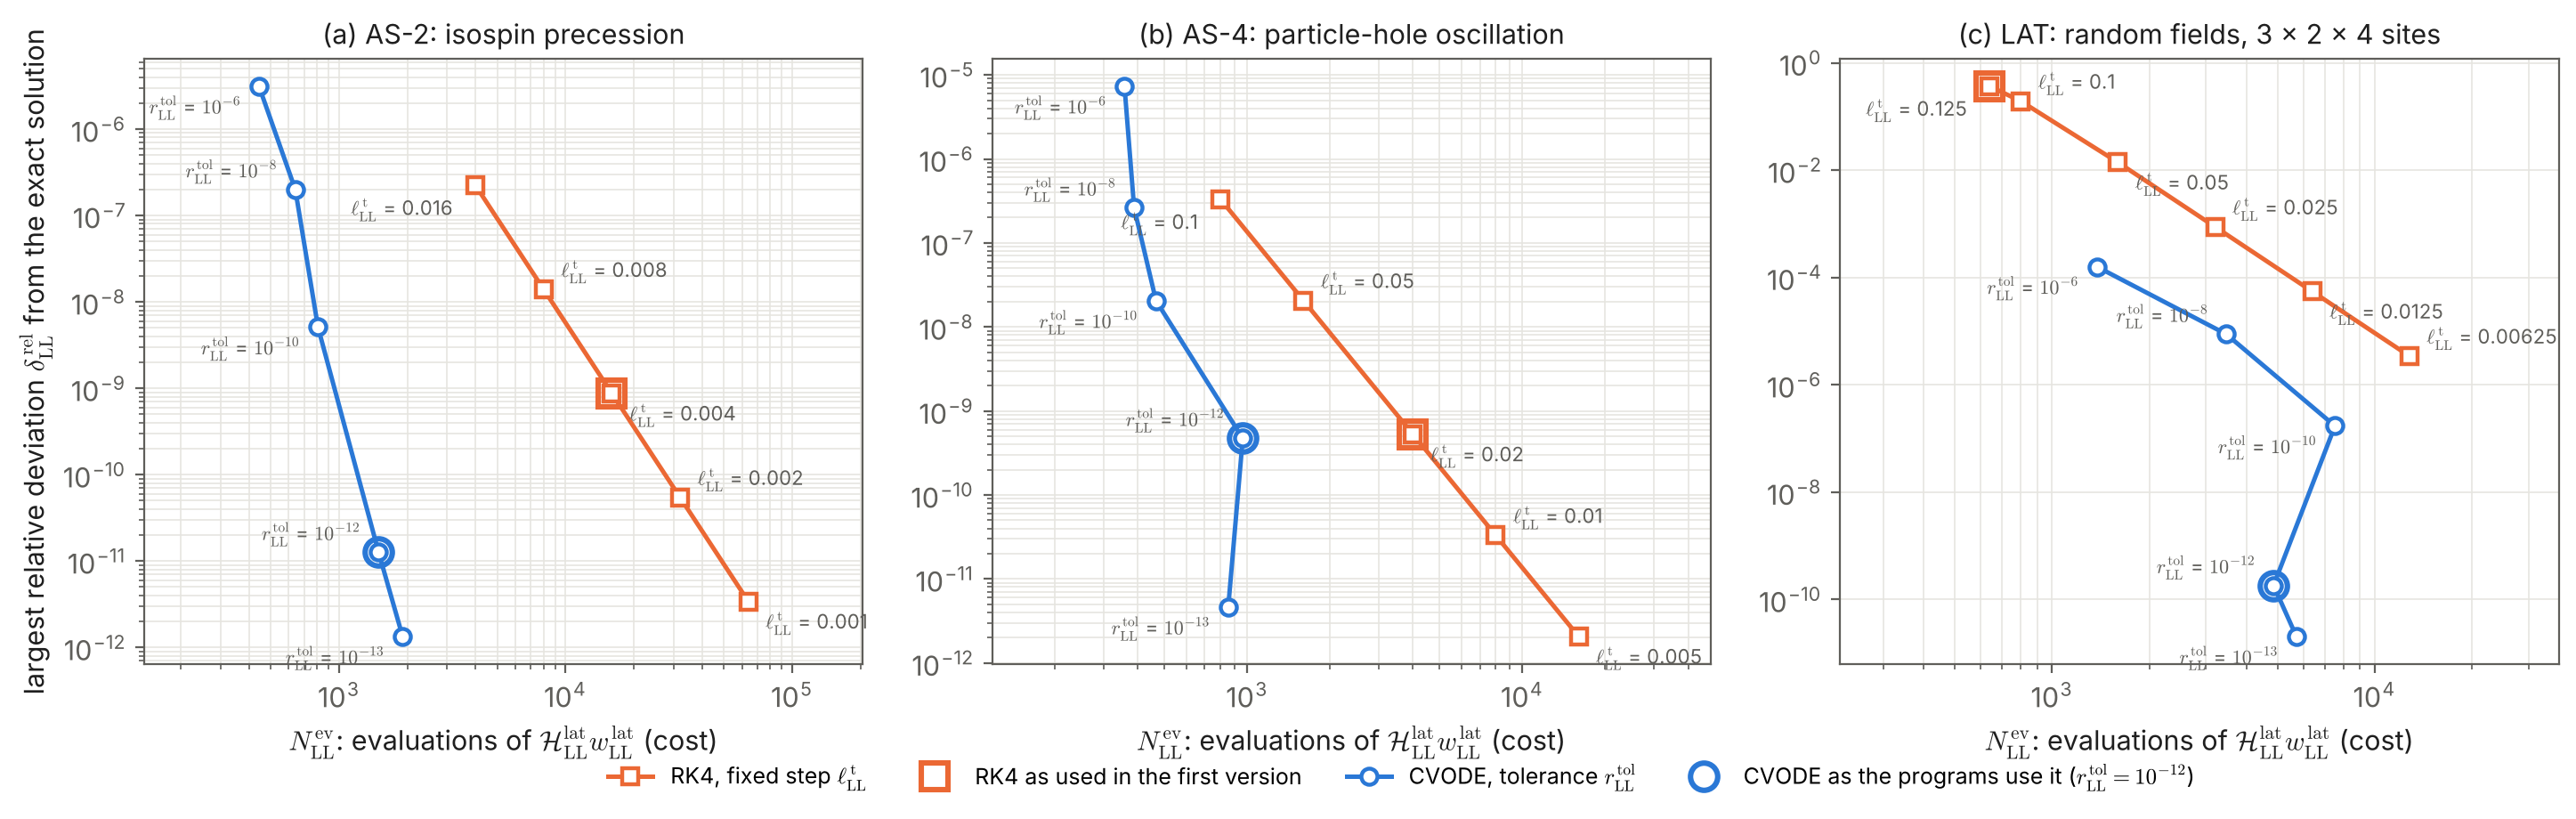
\includegraphics[width=1\textwidth,height=\textheight]{figures/fig_cmp_work_precision.png}

\textbf{Figure 1.} The accuracy against the cost. For each problem the
largest relative deviation \(\delta^{\rm rel}_{\rm LL}\) from the exact
solution against the number \(N^{\rm ev}_{\rm LL}\) of evaluations of
the right side: RK4 (orange squares, one point per fixed step
\(\ell^{\rm t}_{\rm LL}\)) and CVODE (blue circles, one point per
tolerance \(r^{\rm tol}_{\rm LL}\)); the large symbols mark RK4 as the
first version used it and CVODE as the programs use it. Data:
\texttt{test2/cvode\_vs\_rk4/data/cmp\_work\_precision.csv} (program
\texttt{t2\_cvcmp}); figure:
\texttt{test2/cvode\_vs\_rk4/python/make\_cmp\_figures.py}.

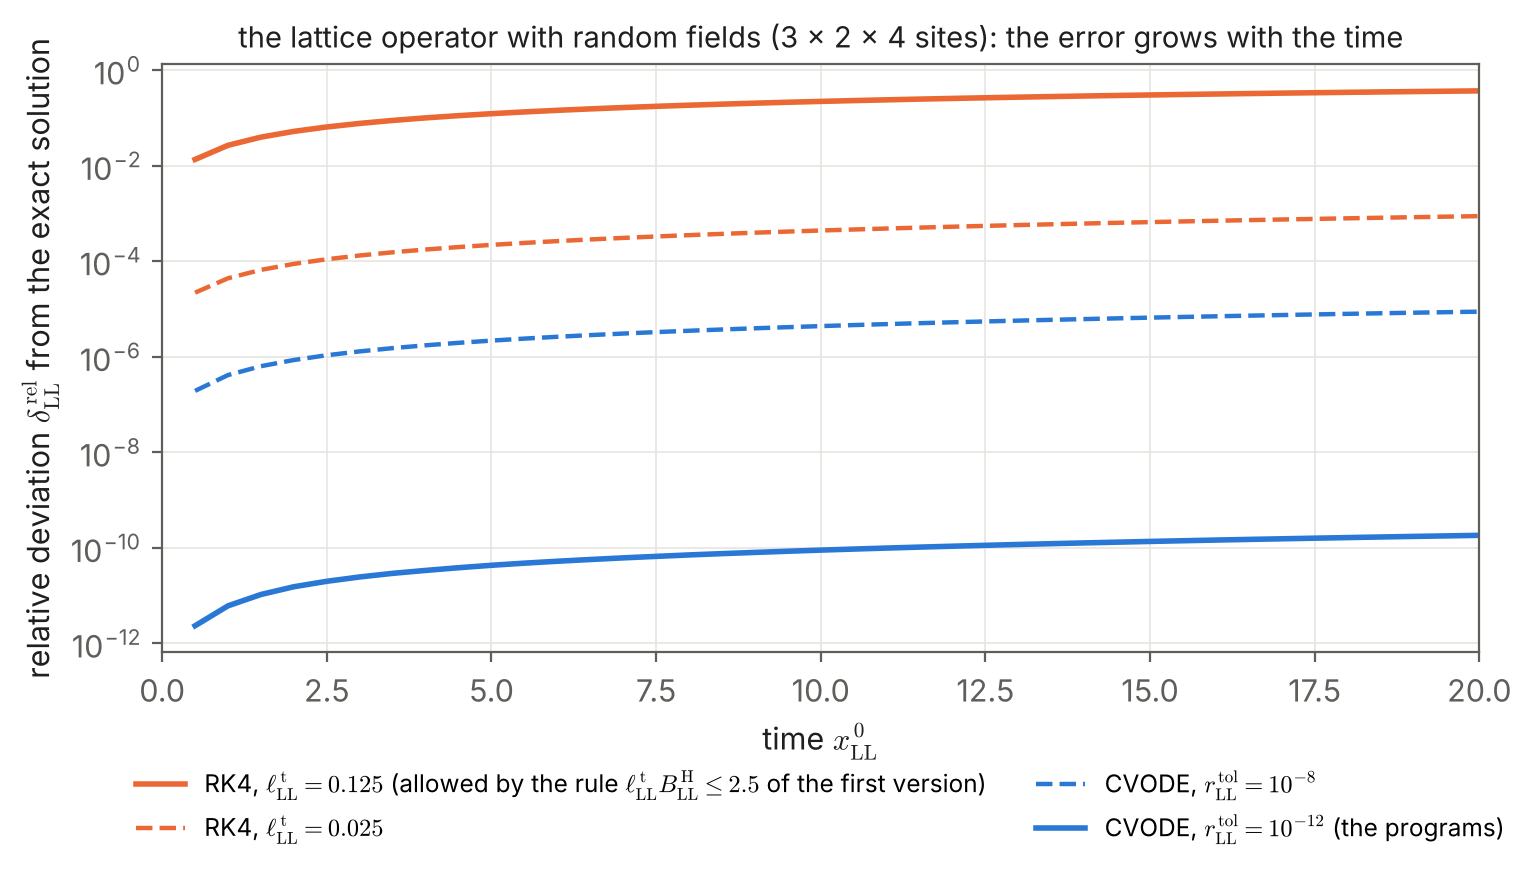
\includegraphics[width=0.8\textwidth,height=\textheight]{figures/fig_cmp_lat_time.png}

\textbf{Figure 2.} The problem LAT: the relative deviation from the
exact solution against the time, for RK4 with the step 0.125 that the
rule of the first version allowed and with 0.025, and for CVODE with
\(r^{\rm tol}_{\rm LL}=10^{-8}\) and \(10^{-12}\). Data:
\texttt{test2/cvode\_vs\_rk4/data/cmp\_lat\_deviation.csv}.

\textbf{What the table and the figures show.} RK4 converges with the
fourth power of the step (halving the step divides the deviation by 16,
as the rows of AS-2 and AS-4 show), so its accuracy is set by the step
chosen; the steps of the first version gave \(10^{-9}\) for AS-2 and
AS-4 because the energies of these problems times the steps are small
(\(\lvert E^{\rm qp}_{{\rm LL},n}\rvert\ell^{\rm t}_{\rm LL}\le0.01\)),
but for LAT, where the energies reach 8.4, the allowed step 0.125 gives
\(\delta^{\rm rel}_{\rm LL}=0.37\). CVODE reaches a prescribed accuracy
without a choice of step: for every problem
\(r^{\rm tol}_{\rm LL}=10^{-12}\) gives \(\delta^{\rm rel}_{\rm LL}\)
between \(10^{-11}\) and \(5\times10^{-10}\). At equal accuracy CVODE
needs 10 times fewer evaluations than RK4 for AS-2 and 4 times fewer for
AS-4; for LAT it needs 7.6 times more evaluations (4856) than RK4 with
the step of the first version (640), which, however, is 37 per cent
wrong; RK4 needs 12800 evaluations (\(\ell^{\rm t}_{\rm LL}=0.00625\))
to reach \(3.4\times10^{-6}\) there. The cost of CVODE does not always
grow monotonically as \(r^{\rm tol}_{\rm LL}\) decreases (LAT at
\(10^{-10}\) needs more evaluations than at \(10^{-12}\)): the
Adams-Moulton formulas of high order have small stability intervals on
the imaginary axis, and the choice of order and step of CVODE then
depends on the tolerance in a non-monotonic way; the accuracy, which is
what the tolerance controls, improves monotonically.

\hypertarget{the-archived-rk4-numbers-are-reproduced}{%
\subsection{5.2 The archived RK4 numbers are
reproduced}\label{the-archived-rk4-numbers-are-reproduced}}

\begin{longtable}[]{@{}
  >{\raggedright\arraybackslash}p{(\columnwidth - 4\tabcolsep) * \real{0.3333}}
  >{\raggedleft\arraybackslash}p{(\columnwidth - 4\tabcolsep) * \real{0.3333}}
  >{\raggedleft\arraybackslash}p{(\columnwidth - 4\tabcolsep) * \real{0.3333}}@{}}
\toprule\noalign{}
\begin{minipage}[b]{\linewidth}\raggedright
quantity (data file)
\end{minipage} & \begin{minipage}[b]{\linewidth}\raggedleft
largest deviation from the exact value, RK4 (first version)
\end{minipage} & \begin{minipage}[b]{\linewidth}\raggedleft
the same, CVODE (\(r^{\rm tol}_{\rm LL}=10^{-12}\))
\end{minipage} \\
\midrule\noalign{}
\endhead
\bottomrule\noalign{}
\endlastfoot
\(P^\uparrow_{\rm LL}\) of AS-2 (\texttt{t2\_A\_precession.csv}) &
5.00e-10 & 1.00e-10 \\
\(P^{\rm h}_{\rm LL}\) of AS-4 (\texttt{t2\_B\_rabi.csv}) & 2.00e-10 &
0.00e0 \\
\end{longtable}

The program \texttt{t2\_cvcmp} reproduces, with its own copy of the RK4
step of the first version, the columns \texttt{P\_up\_rk4} and
\texttt{P\_hole\_rk4} of the archived files
\texttt{t2\_A\_precession.csv} and \texttt{t2\_B\_rabi.csv} to within
half a unit of their 10th decimal (largest differences
\(4.95\times10^{-11}\) and \(4.98\times10^{-11}\), Appendix A): the
archive and the comparison describe the same method. The table above
gives the largest deviation of the printed probabilities of Figures 3(b)
and 4(b) of Test 2 from their exact values, for the first version and
for CVODE.

\hypertarget{the-examples-of-the-solver}{%
\subsection{5.3 The examples of the
solver}\label{the-examples-of-the-solver}}

The four time-dependent examples of \texttt{t2\_solve} were solved with
CVODE at \(r^{\rm tol}_{\rm LL}=10^{-12}\) (the data files of
\texttt{test2/data}) and, by the script \texttt{run\_convergence.sh}, at
\(10^{-10}\) and \(10^{-13}\)
(\(a^{\rm tol}_{\rm LL}=r^{\rm tol}_{\rm LL}/100\); folder
\texttt{test2/cvode\_vs\_rk4/data/conv}). The table gives, column by
column of the time series, the largest difference between the first
version and CVODE at \(10^{-12}\), and between CVODE at the other two
tolerances and CVODE at \(10^{-12}\). When the change from \(10^{-12}\)
to \(10^{-13}\) is much smaller than the difference from the first
version, the CVODE result is converged and the difference is the error
of the first version.

\begin{longtable}[]{@{}
  >{\raggedright\arraybackslash}p{(\columnwidth - 8\tabcolsep) * \real{0.2000}}
  >{\raggedright\arraybackslash}p{(\columnwidth - 8\tabcolsep) * \real{0.2000}}
  >{\raggedleft\arraybackslash}p{(\columnwidth - 8\tabcolsep) * \real{0.2000}}
  >{\raggedleft\arraybackslash}p{(\columnwidth - 8\tabcolsep) * \real{0.2000}}
  >{\raggedleft\arraybackslash}p{(\columnwidth - 8\tabcolsep) * \real{0.2000}}@{}}
\toprule\noalign{}
\begin{minipage}[b]{\linewidth}\raggedright
example
\end{minipage} & \begin{minipage}[b]{\linewidth}\raggedright
column
\end{minipage} & \begin{minipage}[b]{\linewidth}\raggedleft
first version minus CVODE (\(r^{\rm tol}_{\rm LL}=10^{-12}\))
\end{minipage} & \begin{minipage}[b]{\linewidth}\raggedleft
CVODE \(10^{-10}\) minus CVODE \(10^{-12}\)
\end{minipage} & \begin{minipage}[b]{\linewidth}\raggedleft
CVODE \(10^{-13}\) minus CVODE \(10^{-12}\)
\end{minipage} \\
\midrule\noalign{}
\endhead
\bottomrule\noalign{}
\endlastfoot
packet\_free & \texttt{norm} & 1.50e-7 & 1.76e-7 & 3.00e-11 \\
packet\_free & \texttt{E\_expect} & 1.66e-7 & 1.96e-7 & 3.40e-11 \\
packet\_free & \texttt{P\_hole} & 0.00e0 & 0.00e0 & 0.00e0 \\
packet\_free & \texttt{P\_up} & 0.00e0 & 0.00e0 & 0.00e0 \\
packet\_free & \texttt{x\_mean\_1} & 7.75e-6 & 8.63e-8 & 2.00e-10 \\
cyclotron & \texttt{norm} & 2.92e-7 & 7.20e-10 & 2.52e-9 \\
cyclotron & \texttt{E\_expect} & 3.59e-7 & 7.71e-10 & 3.10e-9 \\
cyclotron & \texttt{P\_up} & 0.00e0 & 0.00e0 & 0.00e0 \\
cyclotron & \texttt{x\_mean\_1} & 4.95e-6 & 1.18e-8 & 3.35e-9 \\
cyclotron & \texttt{x\_mean\_2} & 4.52e-6 & 1.36e-8 & 6.27e-9 \\
andreev & \texttt{norm} & 1.46e-9 & 5.60e-11 & 9.00e-12 \\
andreev & \texttt{E\_expect} & 2.79e-9 & 1.29e-10 & 1.61e-11 \\
andreev & \texttt{P\_hole} & 1.40e-9 & 6.20e-11 & 6.00e-12 \\
andreev & \texttt{P\_up} & 1.39e-9 & 6.15e-11 & 6.00e-12 \\
andreev & \texttt{x\_mean\_1} & 5.06e-8 & 1.70e-9 & 4.00e-10 \\
quench & \texttt{abs\_d\_mean} & 4.11e-3 & 4.42e-9 & 4.20e-11 \\
quench & \texttt{abs\_d\_site0} & 4.11e-3 & 4.42e-9 & 4.20e-11 \\
quench & \texttt{N\_F} & 1.27e-8 & 5.07e-7 & 4.90e-9 \\
quench & \texttt{E\_MF} & 1.92e-3 & 3.86e-6 & 3.70e-8 \\
quench & \texttt{ortho\_error} & 4.84e-10 & 2.09e-8 & 1.88e-10 \\
\end{longtable}

\begin{longtable}[]{@{}
  >{\raggedright\arraybackslash}p{(\columnwidth - 12\tabcolsep) * \real{0.1429}}
  >{\raggedleft\arraybackslash}p{(\columnwidth - 12\tabcolsep) * \real{0.1429}}
  >{\raggedleft\arraybackslash}p{(\columnwidth - 12\tabcolsep) * \real{0.1429}}
  >{\raggedleft\arraybackslash}p{(\columnwidth - 12\tabcolsep) * \real{0.1429}}
  >{\raggedleft\arraybackslash}p{(\columnwidth - 12\tabcolsep) * \real{0.1429}}
  >{\raggedleft\arraybackslash}p{(\columnwidth - 12\tabcolsep) * \real{0.1429}}
  >{\raggedleft\arraybackslash}p{(\columnwidth - 12\tabcolsep) * \real{0.1429}}@{}}
\toprule\noalign{}
\begin{minipage}[b]{\linewidth}\raggedright
example
\end{minipage} & \begin{minipage}[b]{\linewidth}\raggedleft
largest change of the norm, RK4 (first version)
\end{minipage} & \begin{minipage}[b]{\linewidth}\raggedleft
the same, CVODE
\end{minipage} & \begin{minipage}[b]{\linewidth}\raggedleft
largest change of the energy, RK4
\end{minipage} & \begin{minipage}[b]{\linewidth}\raggedleft
the same, CVODE
\end{minipage} & \begin{minipage}[b]{\linewidth}\raggedleft
evaluations \(N^{\rm ev}_{\rm LL}\), RK4
\end{minipage} & \begin{minipage}[b]{\linewidth}\raggedleft
the same, CVODE
\end{minipage} \\
\midrule\noalign{}
\endhead
\bottomrule\noalign{}
\endlastfoot
packet\_free & 1.50e-7 & 1.07e-10 & 1.66e-7 & 1.23e-10 & 2400 & 1406 \\
cyclotron & 2.95e-7 & 2.56e-9 & 3.62e-7 & 3.15e-9 & 2880 & 4570 \\
andreev & 1.46e-9 & 9.81e-12 & 2.80e-9 & 1.88e-11 & 4800 & 3514 \\
\end{longtable}

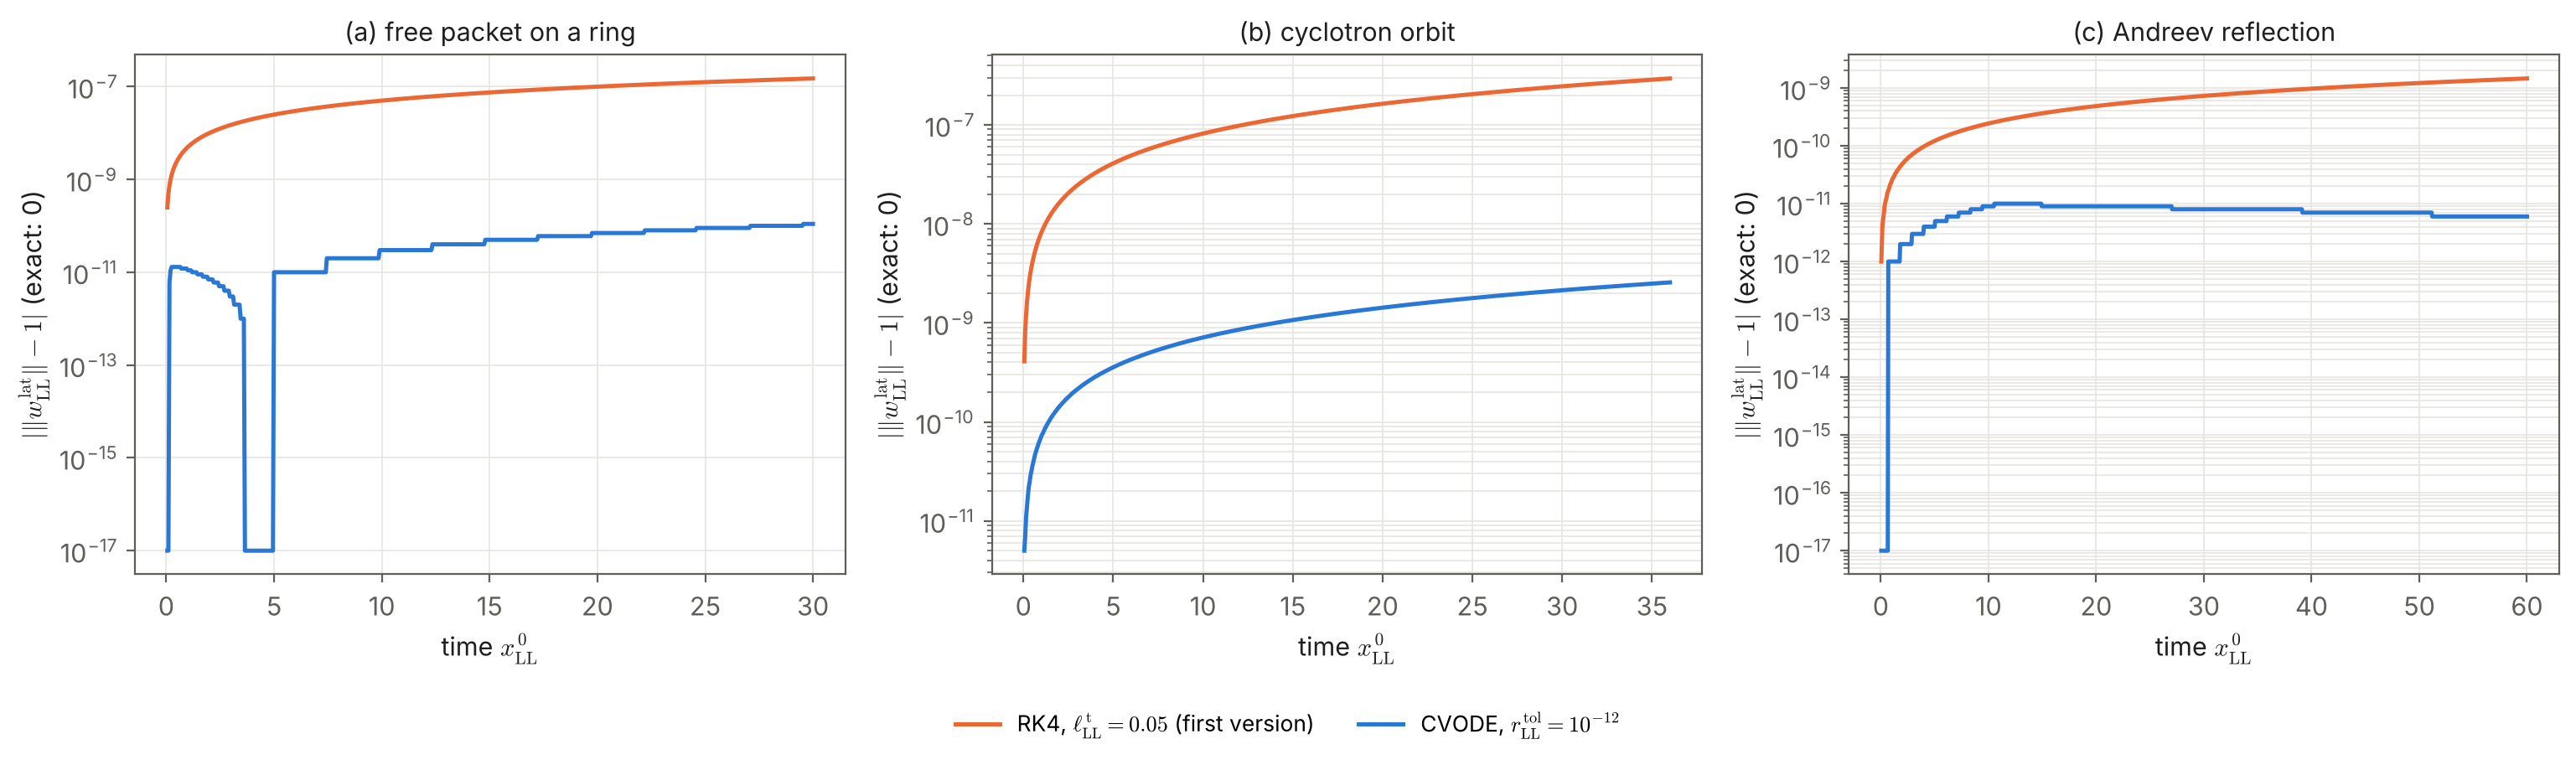
\includegraphics[width=1\textwidth,height=\textheight]{figures/fig_cmp_conservation.png}

\textbf{Figure 3.} The norm of the mode of the three evolve examples,
which the exact evolution conserves: its change
\(\lvert\lVert w^{\rm lat}_{\rm LL}\rVert-1\rvert\) against the time,
for RK4 with \(\ell^{\rm t}_{\rm LL}=0.05\) (first version, orange) and
CVODE with \(r^{\rm tol}_{\rm LL}=10^{-12}\) (blue). Data:
\texttt{test2/rk4\_reference/data/t2\_rs\_*\_series.csv} and
\texttt{test2/data/t2\_rs\_*\_series.csv}, column \texttt{norm}. The
data files print the norm with 12 decimals; the CVODE curves therefore
move in steps of \(10^{-12}\), and where the printed norm is exactly 1
the change is 0 in the printed digits, which the figure draws at
\(10^{-17}\), the lower edge of the panels. The largest changes in the
table above are computed by the programs from the unrounded norm.

The wave packets were computed accurately by the first version (the
centres of the packets differ by at most \(8\times10^{-6}\), the
probabilities by \(1.4\times10^{-9}\)); CVODE conserves the norm and the
energy about 100 to 1400 times better. At
\(r^{\rm tol}_{\rm LL}=10^{-10}\) CVODE is not better than RK4 for
\texttt{packet\_free} (norm change \(1.8\times10^{-7}\)): the default
tolerance \(10^{-12}\) of the programs is needed.

\hypertarget{the-quench-a-correction-of-the-results}{%
\subsection{5.4 The quench: a correction of the
results}\label{the-quench-a-correction-of-the-results}}

\begin{longtable}[]{@{}
  >{\raggedright\arraybackslash}p{(\columnwidth - 8\tabcolsep) * \real{0.2000}}
  >{\raggedleft\arraybackslash}p{(\columnwidth - 8\tabcolsep) * \real{0.2000}}
  >{\raggedleft\arraybackslash}p{(\columnwidth - 8\tabcolsep) * \real{0.2000}}
  >{\raggedleft\arraybackslash}p{(\columnwidth - 8\tabcolsep) * \real{0.2000}}
  >{\raggedleft\arraybackslash}p{(\columnwidth - 8\tabcolsep) * \real{0.2000}}@{}}
\toprule\noalign{}
\begin{minipage}[b]{\linewidth}\raggedright
quantity of the example quench
\end{minipage} & \begin{minipage}[b]{\linewidth}\raggedleft
implicit midpoint rule, \(\ell^{\rm t}_{\rm LL}=0.04\) (first version)
\end{minipage} & \begin{minipage}[b]{\linewidth}\raggedleft
CVODE, \(r^{\rm tol}_{\rm LL}=10^{-10}\)
\end{minipage} & \begin{minipage}[b]{\linewidth}\raggedleft
CVODE, \(r^{\rm tol}_{\rm LL}=10^{-12}\) (programs)
\end{minipage} & \begin{minipage}[b]{\linewidth}\raggedleft
CVODE, \(r^{\rm tol}_{\rm LL}=10^{-13}\)
\end{minipage} \\
\midrule\noalign{}
\endhead
\bottomrule\noalign{}
\endlastfoot
angular frequency of the amplitude oscillation & 1.184485 & 1.188975 &
1.188975 & 1.188975 \\
mean of the gap after the quench & 0.5008765642 & 0.5031251098 &
0.5031251078 & 0.5031251078 \\
amplitude of the oscillation (fit) & 0.00586681 & 0.00707867 &
0.00707867 & 0.00707867 \\
largest change of the conserved functional \(E^{\rm MF}_{\rm LL}\) &
1.92e-3 & 3.96e-6 & 9.69e-8 & 6.00e-8 \\
\end{longtable}

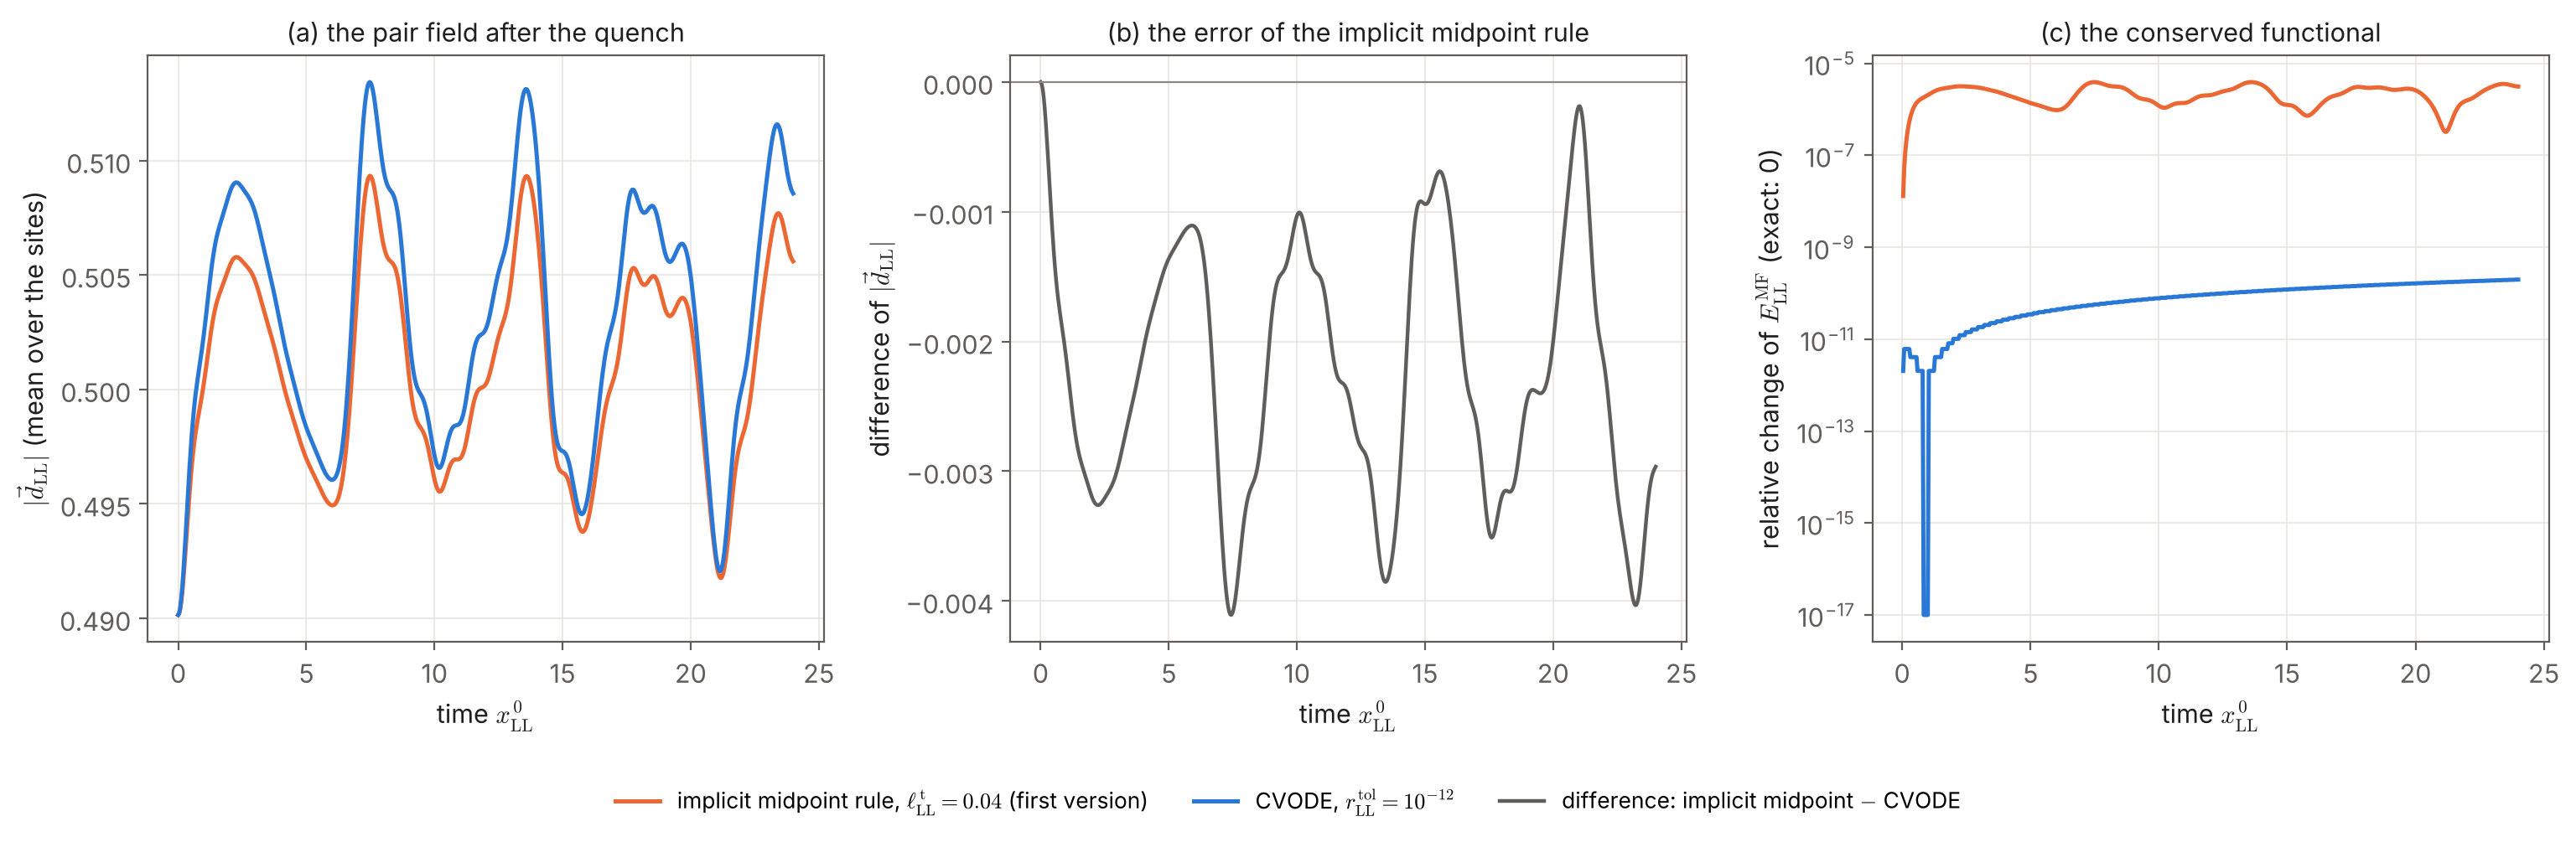
\includegraphics[width=1\textwidth,height=\textheight]{figures/fig_cmp_quench.png}

\textbf{Figure 4.} The quench of the coupling of the uniform superfluid
(24 sites, 192 modes, 73728 complex unknowns): (a) the mean of
\(\lvert d^\iota_{\rm LL}\rvert\) over the sites against the time,
implicit midpoint rule (\(\ell^{\rm t}_{\rm LL}=0.04\), first version)
and CVODE (\(r^{\rm tol}_{\rm LL}=10^{-12}\)); (b) their difference; (c)
the relative change of the conserved functional \(E^{\rm MF}_{\rm LL}\).
Data: \texttt{t2\_rs\_quench\_series.csv} of
\texttt{test2/rk4\_reference/data} and \texttt{test2/data}.

The three CVODE runs agree in the frequency to 6 decimals, in the mean
gap to \(2\times10^{-9}\) and in the amplitude to 8 decimals; the
implicit midpoint rule differs from them by 0.00449 in the frequency
(relative \(3.8\times10^{-3}\)), by 0.00225 in the mean gap (relative
\(4.5\times10^{-3}\); the gap of the new ground state is 0.503114, close
to the CVODE mean 0.503125) and by 17 per cent in the amplitude. The
examples check of the first version compared the frequency with the
amplitude (Higgs) mode of the linearized self-consistent equations,
1.18991 at its mean gap, and found the relative deviation
\(4.56\times10^{-3}\), which it attributed to the terms of second order
in the amplitude and to the weaker modes. The CVODE frequency 1.188975
deviates from that same prediction by \(7.9\times10^{-4}\) only; the
prediction at the CVODE mean gap is computed by the examples check of
the present version (Section 7). The conserved quantities: the midpoint
rule keeps \(N^{\rm F}_{\rm LL}\) and the orthonormality exactly (to
\(10^{-11}\)), but \(E^{\rm MF}_{\rm LL}\) only to \(2\times10^{-3}\);
CVODE keeps \(N^{\rm F}_{\rm LL}\) to \(1.3\times10^{-8}\), the
orthonormality to \(5\times10^{-10}\) and \(E^{\rm MF}_{\rm LL}\) to
\(10^{-7}\).

\hypertarget{the-superfluid-boson-singlet-state-t2_sfbs}{%
\subsection{\texorpdfstring{5.5 The superfluid boson singlet state
(\texttt{t2\_sfbs})}{5.5 The superfluid boson singlet state (t2\_sfbs)}}\label{the-superfluid-boson-singlet-state-t2_sfbs}}

\begin{longtable}[]{@{}
  >{\raggedright\arraybackslash}p{(\columnwidth - 8\tabcolsep) * \real{0.1067}}
  >{\raggedright\arraybackslash}p{(\columnwidth - 8\tabcolsep) * \real{0.3600}}
  >{\raggedleft\arraybackslash}p{(\columnwidth - 8\tabcolsep) * \real{0.1867}}
  >{\raggedleft\arraybackslash}p{(\columnwidth - 8\tabcolsep) * \real{0.1867}}
  >{\raggedleft\arraybackslash}p{(\columnwidth - 8\tabcolsep) * \real{0.1600}}@{}}
\toprule\noalign{}
\begin{minipage}[b]{\linewidth}\raggedright
check
\end{minipage} & \begin{minipage}[b]{\linewidth}\raggedright
quantity
\end{minipage} & \begin{minipage}[b]{\linewidth}\raggedleft
RK4 (first version)
\end{minipage} & \begin{minipage}[b]{\linewidth}\raggedleft
CVODE (\(r^{\rm tol}_{\rm LL}=10^{-12}\))
\end{minipage} & \begin{minipage}[b]{\linewidth}\raggedleft
reference value
\end{minipage} \\
\midrule\noalign{}
\endhead
\bottomrule\noalign{}
\endlastfoot
SB-10 & spectral line of the pair field (pole \(M^{\rm B}_{\rm LL}\)
with the same nodes) & 0.279251576 & 0.279251552 & 0.279251554 \\
SB-10 & relative deviation of the line from the pole & 7.88e-8 & 7.16e-9
& \\
SB-10 & largest relative change of the mean-field energy & 1.50e-8 &
2.30e-9 & 0 \\
SB-16 & line of the gap oscillation, displacement 0.02 & 0.41888388 &
0.41888608 & \\
SB-16 & line of the gap oscillation, displacement 0.01 & 0.41895942 &
0.41896162 & \\
SB-16 & largest relative change of the mean-field energy & 6.80e-7 &
9.60e-10 & 0 \\
\end{longtable}

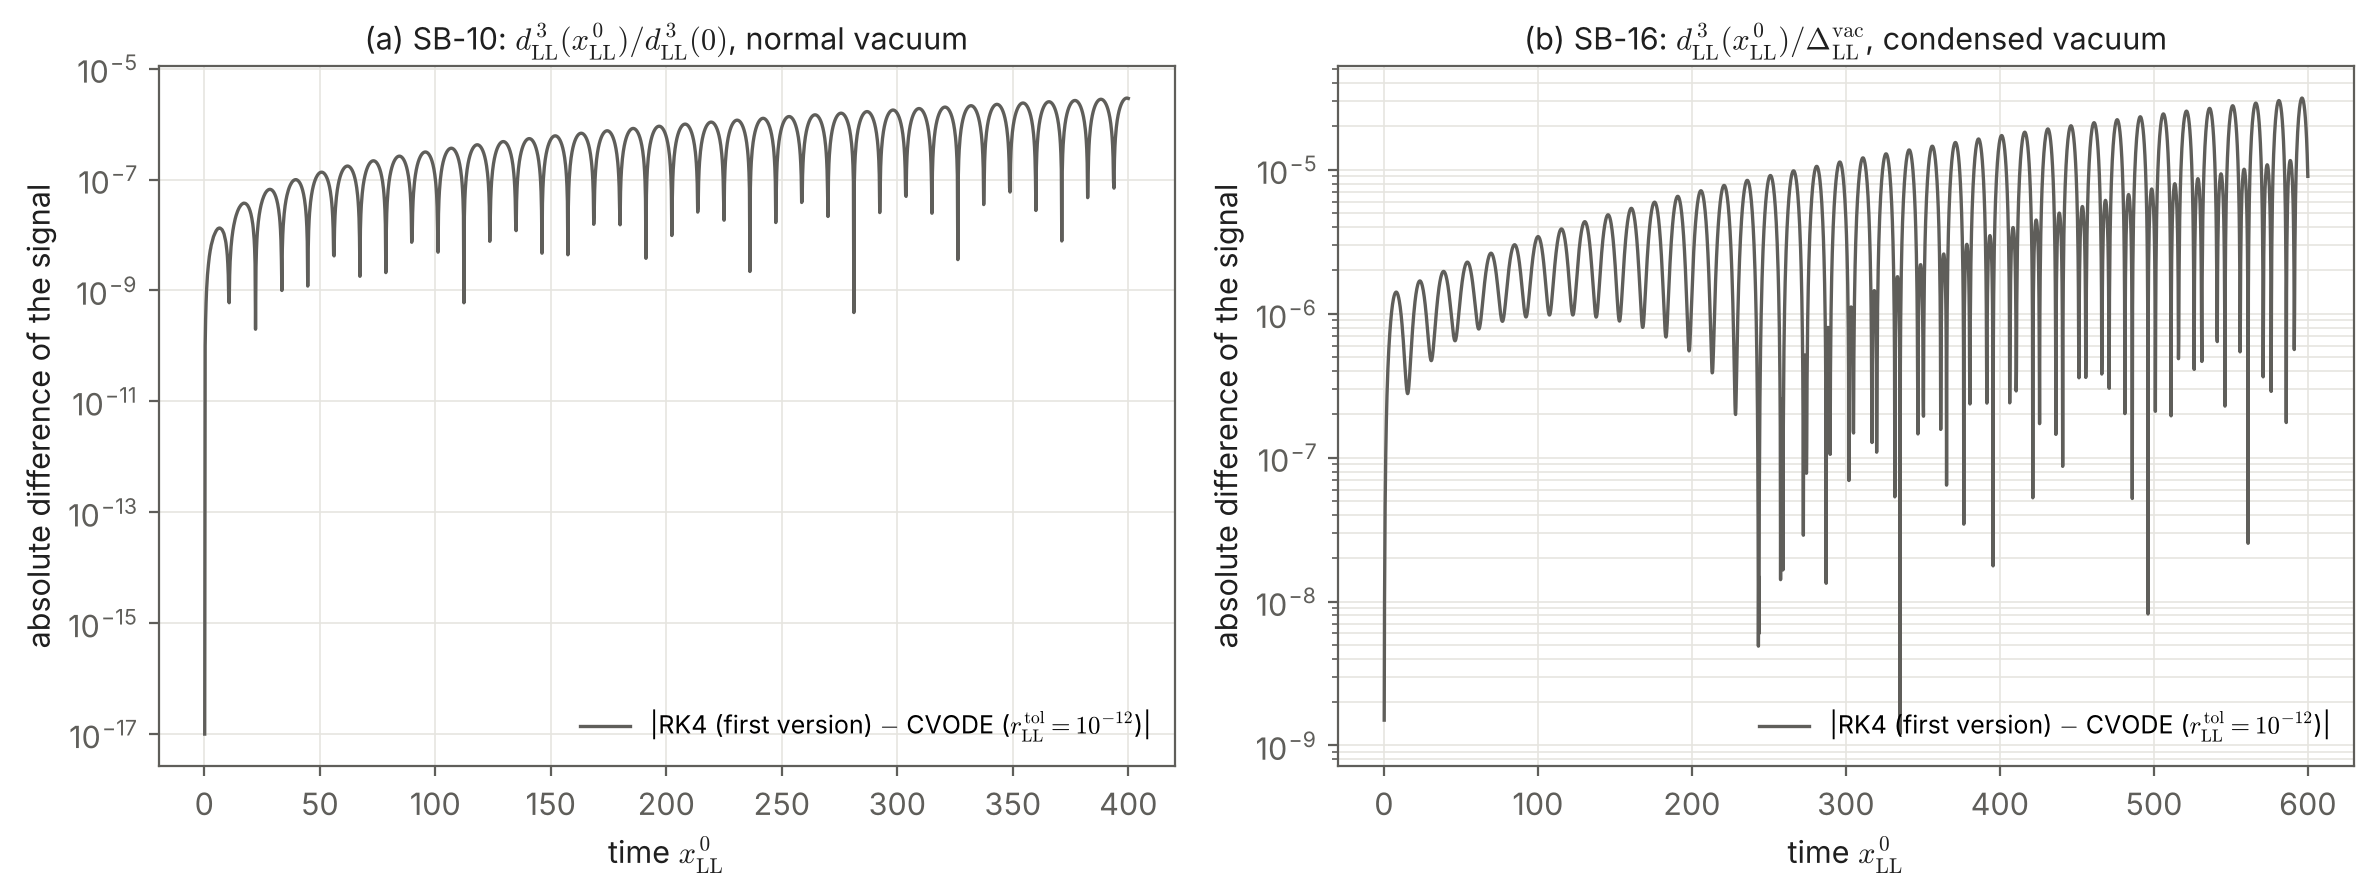
\includegraphics[width=1\textwidth,height=\textheight]{figures/fig_cmp_sfbs.png}

\textbf{Figure 5.} The absolute difference between the signals of RK4
(first version) and CVODE (\(r^{\rm tol}_{\rm LL}=10^{-12}\)) against
the time: (a) SB-10, the pair field of the normal vacuum divided by its
initial value; (b) SB-16, the gap oscillation of the condensed vacuum
divided by \(\Delta^{\rm vac}_{\rm LL}\). Data:
\texttt{t2\_sfbs\_tdbdg\_normal.csv} and
\texttt{t2\_sfbs\_tdbdg\_higgs.csv} of
\texttt{test2/rk4\_reference/data} and \texttt{test2/data}.

The largest differences of the two signals are \(3\times10^{-6}\) and
\(3\times10^{-5}\) (they grow linearly with the time, the accumulated
phase error of RK4); the spectral lines that the checks measure move by
\(2\times10^{-8}\) and \(2\times10^{-6}\), and both checks pass as
before.

\hypertarget{conclusions}{%
\section{6. Conclusions}\label{conclusions}}

\begin{itemize}
\tightlist
\item
  The first version was accurate where the energies times the step were
  small (AS-2, AS-4, the wave packets, SB-10, SB-16); its numbers there
  are confirmed by CVODE within \(10^{-6}\) or better.
\item
  The first version was inaccurate for the quench (relative errors of
  the frequency, of the mean gap and of the amplitude of the amplitude
  oscillation: \(3.8\times10^{-3}\), \(4.5\times10^{-3}\) and 17 per
  cent), and its time-step rule allowed steps with which RK4 is useless
  on lattices with large energies (problem LAT: 37 per cent).
\item
  CVODE controls the error by its tolerances; with
  \(r^{\rm tol}_{\rm LL}=10^{-12}\) and
  \(a^{\rm tol}_{\rm LL}=10^{-14}\) every result of Test 2 is converged
  to the printed digits, as the three tolerances of Section 5.3 show.
\end{itemize}

\hypertarget{status-of-the-work-and-how-to-reproduce-it}{%
\section{7. Status of the work and how to reproduce
it}\label{status-of-the-work-and-how-to-reproduce-it}}

\textbf{Done:} the vendored SUNDIALS; \texttt{t2core::cvode}; the Rust
programs \texttt{t2\_analytic}, \texttt{t2\_fields}, \texttt{t2\_solve},
\texttt{t2\_sfbs}, \texttt{t2\_plot} with CVODE; the Python solver
\texttt{t2\_solve.py} with the same CVODE through the shared library
\texttt{libt2cvode}; all data files and figures of Test 2; the documents
of Test 2 and of the folder Revision\_SuperLoop; the comparison program
\texttt{t2\_cvcmp}, the convergence runs and the figures of this
document; the registry entries of the new symbols. \textbf{Following
steps:} the notebook \texttt{3+1super-loop.nb} (its time integrations
with a SUNDIALS method of the Wolfram Language), then the older code of
the repository that integrates in time with a fixed-step method.

On the Mac (Terminal), from the folder of the repository:

\begin{Shaded}
\begin{Highlighting}[]
\BuiltInTok{cd} \StringTok{"/Users/nsh/Developer/github/spacetimes/Revision\_SuperLoop/test2/rust"}
\ExtensionTok{cargo}\NormalTok{ build }\AttributeTok{{-}{-}release}
\ControlFlowTok{for}\NormalTok{ p }\KeywordTok{in}\NormalTok{ t2\_fields t2\_analytic t2\_sfbs}\KeywordTok{;} \ControlFlowTok{do} \ExtensionTok{./target/release/}\VariableTok{$p}\KeywordTok{;} \ControlFlowTok{done}
\BuiltInTok{cd}\NormalTok{ ..}
\ControlFlowTok{for}\NormalTok{ n }\KeywordTok{in}\NormalTok{ packet\_free cyclotron andreev kink\_spectrum ground\_state kink\_ground\_state quench}\KeywordTok{;} \ControlFlowTok{do}
  \ExtensionTok{./rust/target/release/t2\_solve}\NormalTok{ examples/}\VariableTok{$n}\NormalTok{.t2in }\AttributeTok{{-}{-}out}\NormalTok{ data/t2\_rs\_}\VariableTok{$n}
  \ExtensionTok{python3}\NormalTok{ python/t2\_solve.py examples/}\VariableTok{$n}\NormalTok{.t2in }\AttributeTok{{-}{-}out}\NormalTok{ data/t2\_py\_}\VariableTok{$n}
\ControlFlowTok{done}
\FunctionTok{bash}\NormalTok{ cvode\_vs\_rk4/run\_convergence.sh }\StringTok{"}\VariableTok{$PWD}\StringTok{/rust/target/release/t2\_solve"}
\ExtensionTok{./rust/target/release/t2\_cvcmp}
\BuiltInTok{cd}\NormalTok{ .. }\KeywordTok{\&\&} \ExtensionTok{python3}\NormalTok{ test2/cvode\_vs\_rk4/python/make\_cmp\_figures.py}
\end{Highlighting}
\end{Shaded}

The first two lines build every program of Test 2 and the shared library
\texttt{libt2cvode} of the Python solver (the vendored SUNDIALS is
compiled with them); the loop runs the three check programs, the next
loop the seven examples of both solvers; \texttt{run\_convergence.sh}
solves the four time-dependent examples at the tolerances \(10^{-10}\)
and \(10^{-13}\); \texttt{t2\_cvcmp} writes the comparison (it exits
with status 1 if one of its checks fails); the last line draws the five
figures. The programs write their outputs into the folders named in the
text.

\hypertarget{the-files-of-the-comparison}{%
\section{8. The files of the
comparison}\label{the-files-of-the-comparison}}

\begin{longtable}[]{@{}
  >{\raggedright\arraybackslash}p{(\columnwidth - 2\tabcolsep) * \real{0.5435}}
  >{\raggedright\arraybackslash}p{(\columnwidth - 2\tabcolsep) * \real{0.4565}}@{}}
\toprule\noalign{}
\begin{minipage}[b]{\linewidth}\raggedright
file (in the folder \texttt{Revision\_SuperLoop/test2})
\end{minipage} & \begin{minipage}[b]{\linewidth}\raggedright
content
\end{minipage} \\
\midrule\noalign{}
\endhead
\bottomrule\noalign{}
\endlastfoot
\texttt{cvode\_vs\_rk4/P\_CVODE\_vs\_RK4.src.md} & the hand-written
source of this document (the assembly inserts the symbol table, the
tables of Section 5, the report, the code and this list) \\
\texttt{rust/t2core/src/cvode.rs} & the module of the time integration
with CVODE (library t2core) \\
\texttt{rust/t2core/src/lib.rs} & the library t2core: its list of
modules \\
\texttt{rust/t2core/src/lattice.rs} & the lattice operator (its RK4 step
removed) \\
\texttt{rust/t2core/Cargo.toml} & the manifest of t2core (dependency on
the vendored crate cvode\_rs) \\
\texttt{rust/t2analytic/src/main.rs} & the program t2\_analytic (AS-2
and AS-4 with CVODE) \\
\texttt{rust/t2fields/src/main.rs} & the program t2\_fields (GS-13:
CVODE against the exact spectral solution) \\
\texttt{rust/t2solve/src/main.rs} & the solver t2\_solve (tasks evolve
and quench with CVODE) \\
\texttt{rust/t2solve/src/input.rs} & the input format t2in 2 of the
solver \\
\texttt{rust/t2solve/src/ops.rs} & the operators of the solver \\
\texttt{rust/t2sfbs/src/main.rs} & the program t2\_sfbs (SB-10, SB-16
with CVODE) \\
\texttt{rust/t2plot/src/main.rs} & the plotting program t2\_plot \\
\texttt{rust/Cargo.toml} & the manifest of the workspace of Test 2 \\
\texttt{rust/Cargo.lock} & the locked versions of the crates \\
\texttt{rust/t2cvode\_c/Cargo.toml} & the manifest of the shared library
libt2cvode \\
\texttt{rust/t2cvode\_c/src/lib.rs} & the C interface of t2core::cvode
(the shared library libt2cvode of the Python solver) \\
\texttt{python/t2\_solve.py} & the Python solver (tasks evolve and
quench with CVODE through libt2cvode) \\
\texttt{python/t2\_examples\_check.py} & the checks EX-1 to EX-8 of the
examples \\
\texttt{python/t2\_plot.py} & the Python plotter of the solutions \\
\texttt{python/make\_t2\_figures.py} & the figures of items {[}1{]} and
{[}2{]} of Test 2 (Figure 2: CVODE, check GS-13) \\
\texttt{../../vendor/sundials\_rs-7.8.0/SHA256SUMS.txt} & the digests of
the 283 vendored files of SUNDIALS 7.8.0 in Rust \\
\texttt{rust/t2cvcmp/src/main.rs} & the comparison program t2\_cvcmp \\
\texttt{rust/t2cvcmp/Cargo.toml} & its manifest \\
\texttt{cvode\_vs\_rk4/run\_convergence.sh} & the convergence runs of
the solver examples \\
\texttt{cvode\_vs\_rk4/python/make\_cmp\_figures.py} & the figures of
this document \\
\texttt{cvode\_vs\_rk4/tools/assemble\_provenance.py} & this assembly of
the document \\
\texttt{cvode\_vs\_rk4/tools/build\_docs.sh} & the conversion .md
-\textgreater{} .tex -\textgreater{} .pdf \\
\texttt{cvode\_vs\_rk4/tools/doc\_header.tex} & the LaTeX header of the
conversion \\
\texttt{cvode\_vs\_rk4/data/cmp\_report.txt} & the report of t2\_cvcmp
(Appendix A) \\
\texttt{cvode\_vs\_rk4/data/cmp\_tables.md} & the tables of Section 5,
written by t2\_cvcmp \\
\texttt{cvode\_vs\_rk4/data/cmp\_work\_precision.csv} & the runs of
Section 5.1 (Figure 1) \\
\texttt{cvode\_vs\_rk4/data/cmp\_lat\_deviation.csv} & the deviation of
LAT against the time (Figure 2) \\
\texttt{cvode\_vs\_rk4/data/cmp\_series\_differences.csv} & the
differences of the time series (Sections 5.3, 5.5) \\
\texttt{rk4\_reference/SHA256SUMS\_data.txt} & the digests of the 106
archived data files of the first version \\
\texttt{cvode\_vs\_rk4/data/conv/} (36 files) & the convergence runs of
the solver (Section 5.3): for each of the four examples and each of the
tolerances \(10^{-10}\) and \(10^{-13}\) the input file \texttt{.t2in},
the fields, the time series and the summary \\
\texttt{cvode\_vs\_rk4/figures/} (10 files) & the five figures of this
document, each as \texttt{.pdf} and \texttt{.png} \\
\end{longtable}

The SHA-256 digests of these files (each line: the digest, two spaces,
the path in the folder \texttt{Revision\_SuperLoop/test2}; the command
\texttt{sha256sum\ -c} on Linux, or \texttt{shasum\ -a\ 256\ -c} on
macOS, run in that folder with these lines as input, checks them):

\begin{Shaded}
\begin{Highlighting}[]
\NormalTok{9daa10d19e02cdde6717421969fbab4272f7545d7a9eb553879c58f6e81b9bea  cvode\_vs\_rk4/P\_CVODE\_vs\_RK4.src.md}
\NormalTok{4d1f93b147745574fd24b0713b0fb1619c14e7b3274980ba05ed1474343e08e5  rust/t2core/src/cvode.rs}
\NormalTok{5ffa38243c640b9a0c56f599bd823d009f100d766827241d5bb916b2aa062489  rust/t2core/src/lib.rs}
\NormalTok{dab79f76867469c867f54f7596f5afe3541ff13ac20055e213fc1485b6770783  rust/t2core/src/lattice.rs}
\NormalTok{4e8d8ca5c485c44a0dbf8392db86f98b4b3539ad4c6dae7cc9e4e1146c5423c1  rust/t2core/Cargo.toml}
\NormalTok{8fb5ad97b0919f63a06d573f1d51ed92c65bf9e4cef05e79d35c7f270d75d795  rust/t2analytic/src/main.rs}
\NormalTok{50b9903c673b420ba4ff1ef52d12fd4ba0b147628a01b9be687a26d182d0dbcf  rust/t2fields/src/main.rs}
\NormalTok{51ece54663942a06f2d506cc703e821c2e9d6398fe3557ba2448c1415ef14435  rust/t2solve/src/main.rs}
\NormalTok{496582dcac974a071fcdf5f512d6d6541c54168576433bafbec7fa34c6f77109  rust/t2solve/src/input.rs}
\NormalTok{ffbf4d84fc45f3b37efa79167881d99ec83557ad646beebd07da78eafcfa13da  rust/t2solve/src/ops.rs}
\NormalTok{e45d9db743d3954fe9ea282fbd5505b7c74bf6974842c6500e035e6a1fddb787  rust/t2sfbs/src/main.rs}
\NormalTok{aa740ea0100c9dfc5b8e9986c5d3caf28f84d558a199b3275133b879f06f063f  rust/t2plot/src/main.rs}
\NormalTok{0ff87a48b052eff6d5a8ec48d62b89a117fd354ce88d43d1600ca8088f92237a  rust/Cargo.toml}
\NormalTok{b74a42a7acf5ce394fb82e5fa379fd7b839fdcb6665f7a4a63cc9966b9d15109  rust/Cargo.lock}
\NormalTok{c8ef47dadc0f3a764969e9078d291b56d1fda6214c5b287dd3701478a546381e  rust/t2cvode\_c/Cargo.toml}
\NormalTok{01c1d1ba6b299c3cab31973e2406850af688a900e3f439c2833529ac000462bb  rust/t2cvode\_c/src/lib.rs}
\NormalTok{331b07273d2479c125d98ae081d3fd111abac02a82c81cc1c089a6633e8b1d58  python/t2\_solve.py}
\NormalTok{643f9b6a5a0f716dac48f228a7778fa22431f3b08e00c8b852e609630ba6152a  python/t2\_examples\_check.py}
\NormalTok{e5ec0c5d264889a06265e021bbf5ce540bb56a011f005fa2f4453e89ef0d70e6  python/t2\_plot.py}
\NormalTok{d5d38db002c97ab373693decf46f1e112a141273cad50b0611a2831ef161d9ad  python/make\_t2\_figures.py}
\NormalTok{a062365c7cc9f0e4bad502b9d5fc0a51d16dee868ef2edfee9bfd92ded3de94c  ../../vendor/sundials\_rs{-}7.8.0/SHA256SUMS.txt}
\NormalTok{11ac2ecd6a36d5b8f5323e7a3e13b9ad476cdd2b72c89099a0015e8ee352dc54  rust/t2cvcmp/src/main.rs}
\NormalTok{bb6ec652913d355b2857746b223c186278923f631428b2633444156be19e9dd9  rust/t2cvcmp/Cargo.toml}
\NormalTok{74ab8cda1fe469b7d71651cd2847fcb2a41076cf7cae08a957de19b45e40bd34  cvode\_vs\_rk4/run\_convergence.sh}
\NormalTok{3a48b57f9f6a5b69ce2c6d507107a93f87f23b446308091dd3a5c705cbe25537  cvode\_vs\_rk4/python/make\_cmp\_figures.py}
\NormalTok{3a5f7205f573fdae845c1f4cec3768bef74bf9d996b6750e2efa20a74589c33f  cvode\_vs\_rk4/tools/assemble\_provenance.py}
\NormalTok{f5e38096826890c64580c3c5964c7db643e17611a08a1b87c48771dbcdf4d421  cvode\_vs\_rk4/tools/build\_docs.sh}
\NormalTok{d7ca078f2469605306af331e68a8f2526149a197441f15230b00cc6f35395320  cvode\_vs\_rk4/tools/doc\_header.tex}
\NormalTok{48e69b803c0d8b8a1d8f3bc93960b986d8c1a8c0fdb0f05166b99cca84f980ee  cvode\_vs\_rk4/data/cmp\_report.txt}
\NormalTok{372e72ad62dd5e7ec5dff3955edde2585c5a9edce9bfcfc3d76aa7ac9474f562  cvode\_vs\_rk4/data/cmp\_tables.md}
\NormalTok{fea0faf35475c6e7318668dd0db6642e6e328d8fe26e68ed12c7375f1425deae  cvode\_vs\_rk4/data/cmp\_work\_precision.csv}
\NormalTok{4d15f7c94146c14ec1773e5db089ee2428a3d1b70dd8b7824f7fed1570df590e  cvode\_vs\_rk4/data/cmp\_lat\_deviation.csv}
\NormalTok{41c24ed19df3a6dd1179b6b31bd3985d7a87acde295ef372905fe03e766c6520  cvode\_vs\_rk4/data/cmp\_series\_differences.csv}
\NormalTok{55fa65783cedfcb1af6275515025be90c8ca863a0418166ca9580dea7913e410  rk4\_reference/SHA256SUMS\_data.txt}
\NormalTok{46310bbd846f8501e686c0200c9cd7324ddf36c4d462dab754e716c38eecf17e  cvode\_vs\_rk4/data/conv/andreev\_rtol1e{-}10.t2in}
\NormalTok{0f885e0bcea41ec0fc24769b8ea16b6f5828b4d49e5c31124a14a041acd08877  cvode\_vs\_rk4/data/conv/andreev\_rtol1e{-}10\_fields.csv}
\NormalTok{bc1419cdcdab70e2497efbcf66d457676b8f297cd4fd37b266f107f428b38214  cvode\_vs\_rk4/data/conv/andreev\_rtol1e{-}10\_series.csv}
\NormalTok{22c9920004678f509e6fcddf2d9800f4ba8907e32bfb77511e2919035347f6c5  cvode\_vs\_rk4/data/conv/andreev\_rtol1e{-}10\_summary.txt}
\NormalTok{e4375430cf22436d49cb358490f63f2559954274a5fa77fb6eaaf98514a94269  cvode\_vs\_rk4/data/conv/andreev\_rtol1e{-}13.t2in}
\NormalTok{61a91f729af99e943678a3fc00ebbde53b2f5d125b3f0ccfa8fde70162cfe15b  cvode\_vs\_rk4/data/conv/andreev\_rtol1e{-}13\_fields.csv}
\NormalTok{c62eb09c720f50376daf0805240ef64da25b94adb1992e0bd599e0fc69416cf3  cvode\_vs\_rk4/data/conv/andreev\_rtol1e{-}13\_series.csv}
\NormalTok{bd98d65eef6a58420879fdf5ace395b8eeb6d774e2ef3d21d25f093b31dd56e2  cvode\_vs\_rk4/data/conv/andreev\_rtol1e{-}13\_summary.txt}
\NormalTok{0c25103622adf74bca4870389031dd4bec37dbb5ea2a9d1ed36d84f77d8e8a0e  cvode\_vs\_rk4/data/conv/cyclotron\_rtol1e{-}10.t2in}
\NormalTok{32e11f6ec6875b94e3ccca982cf9e4273845b22e6f838035583d8d8bcd27b639  cvode\_vs\_rk4/data/conv/cyclotron\_rtol1e{-}10\_fields.csv}
\NormalTok{4517cc1238bd38857f81f4967fb998bd6f836dd829a4ef8f434a8fba900300bc  cvode\_vs\_rk4/data/conv/cyclotron\_rtol1e{-}10\_series.csv}
\NormalTok{842327310444b0d866184cc4618072e1d9378a643cc056e37789c7ff41080567  cvode\_vs\_rk4/data/conv/cyclotron\_rtol1e{-}10\_summary.txt}
\NormalTok{edce3fed5a9445b220b8f013a7e2f1d4663b8aebbc2689ed823729f75d6a2a66  cvode\_vs\_rk4/data/conv/cyclotron\_rtol1e{-}13.t2in}
\NormalTok{45881806e19f3b98615fabf762baefe8bcb8ecdf9cece6f9392c7589290579d2  cvode\_vs\_rk4/data/conv/cyclotron\_rtol1e{-}13\_fields.csv}
\NormalTok{7038c61df1a3b4a3217f4acfa8df1bb62e610d793cd96f2bbb11662699aaff7c  cvode\_vs\_rk4/data/conv/cyclotron\_rtol1e{-}13\_series.csv}
\NormalTok{31b6074a85c5221e209ca6ff938d6ce97a7ded19e6c72d7b6731ba0d185a3016  cvode\_vs\_rk4/data/conv/cyclotron\_rtol1e{-}13\_summary.txt}
\NormalTok{4f529989b9fada4f1dd6e4d2c5e84cbff3b867e4ca5d44e474c634953bcf8ce6  cvode\_vs\_rk4/data/conv/packet\_free\_rtol1e{-}10.t2in}
\NormalTok{12a56df2793143cceb307518c1d7a951c89331c3f10db9b99e26702e940aee56  cvode\_vs\_rk4/data/conv/packet\_free\_rtol1e{-}10\_fields.csv}
\NormalTok{5d3e6de60bd827055f738a3cf1a8171e98fbe22c20498e5d1e537e0bc2e88f47  cvode\_vs\_rk4/data/conv/packet\_free\_rtol1e{-}10\_series.csv}
\NormalTok{5af1e8bdc9433b57b7b0c0170065ab7fe133971887f334268064d361b8e1340e  cvode\_vs\_rk4/data/conv/packet\_free\_rtol1e{-}10\_summary.txt}
\NormalTok{3de6b714810579af5f23778b941c3cbd6976ae6b0d817f8823cd0f548eb38cd3  cvode\_vs\_rk4/data/conv/packet\_free\_rtol1e{-}13.t2in}
\NormalTok{03ac0010bfa50139ce34fa7b2e6d6508ad0732a9992c2da4b7c03318fcf7d56c  cvode\_vs\_rk4/data/conv/packet\_free\_rtol1e{-}13\_fields.csv}
\NormalTok{1e032e75564f3fc0f4e2b159d2c752d8c5b9e21382edf2dc1807f9675bd7e3c4  cvode\_vs\_rk4/data/conv/packet\_free\_rtol1e{-}13\_series.csv}
\NormalTok{d9e90014ec6b5d51b800f0e947eb43e5735566d6cff5b1cc950e8d4cfb48ddc1  cvode\_vs\_rk4/data/conv/packet\_free\_rtol1e{-}13\_summary.txt}
\NormalTok{2f92bbf302825e10e8d26c4e2e86ad785dc6dd73907c786aeb04c6fba4193679  cvode\_vs\_rk4/data/conv/quench\_rtol1e{-}10.t2in}
\NormalTok{a9a67107b4d3bcc73a2e068071b2f27ee1229210ed86e075149d8e943412e31b  cvode\_vs\_rk4/data/conv/quench\_rtol1e{-}10\_fields.csv}
\NormalTok{fedf30fa15f587b6da6e0f5ba98ecaa4bc924e20e68920b4ba797c215de66ea7  cvode\_vs\_rk4/data/conv/quench\_rtol1e{-}10\_iterations.csv}
\NormalTok{2e755102bae80ec636a04d65e4fea75b689f141b421854662fe2ba113c93424c  cvode\_vs\_rk4/data/conv/quench\_rtol1e{-}10\_series.csv}
\NormalTok{9b391bb8c06355e07562835d407212cedc8ed83ab0960786bf803be010c25f4f  cvode\_vs\_rk4/data/conv/quench\_rtol1e{-}10\_spectrum.csv}
\NormalTok{9c013fc57e0041abc1201a4f9b6fd80c1cd9bbb1e74a2a84c949c97c2c29f102  cvode\_vs\_rk4/data/conv/quench\_rtol1e{-}10\_summary.txt}
\NormalTok{1fc4629bc3d0ad5d895397ff147de6b63ba7412fecc665fe13c89a8771767ca8  cvode\_vs\_rk4/data/conv/quench\_rtol1e{-}13.t2in}
\NormalTok{ab787e259c9fb52450d27f347a8c43a8b35e07f76a4e789e200ce5bb0c7b7f99  cvode\_vs\_rk4/data/conv/quench\_rtol1e{-}13\_fields.csv}
\NormalTok{fedf30fa15f587b6da6e0f5ba98ecaa4bc924e20e68920b4ba797c215de66ea7  cvode\_vs\_rk4/data/conv/quench\_rtol1e{-}13\_iterations.csv}
\NormalTok{c25e8c26476f8963c6c6dbbe0d2afe13ba5816e214dd99d36cd98f075be0a8bd  cvode\_vs\_rk4/data/conv/quench\_rtol1e{-}13\_series.csv}
\NormalTok{9b391bb8c06355e07562835d407212cedc8ed83ab0960786bf803be010c25f4f  cvode\_vs\_rk4/data/conv/quench\_rtol1e{-}13\_spectrum.csv}
\NormalTok{4d2baa00e10cae3916211806d1e84c3e32063abc91c5ef3836ce44f99df03f36  cvode\_vs\_rk4/data/conv/quench\_rtol1e{-}13\_summary.txt}
\NormalTok{d747e55e0a28372a37743eaf32407fb9bbb3116088dcd4d9d9861e25e5f5a10d  cvode\_vs\_rk4/figures/fig\_cmp\_conservation.pdf}
\NormalTok{9764badfd131b386853c3c5301eb62155cb038f5caab81b7e8ba2d4a852625af  cvode\_vs\_rk4/figures/fig\_cmp\_conservation.png}
\NormalTok{6c184842e0457e139cf421b5c4cf08a6ad05efd185527695d702bd258cb5f110  cvode\_vs\_rk4/figures/fig\_cmp\_lat\_time.pdf}
\NormalTok{5ab90d13d08e79585a679043ac6aa4ec379f723fcb074737982a4b1514ddf7df  cvode\_vs\_rk4/figures/fig\_cmp\_lat\_time.png}
\NormalTok{846a54a99635f9908cec20bbbb0b93fcb76d6f8c4868d8b50f4af39999420b5d  cvode\_vs\_rk4/figures/fig\_cmp\_quench.pdf}
\NormalTok{4ce9a92498c1f9b8287576a7d642d4802aecacf11ea489815c3bb634a70f8c84  cvode\_vs\_rk4/figures/fig\_cmp\_quench.png}
\NormalTok{0e30c0837ea30f071ec7b55ba40c605bbebe14f43d25fcb22bff67b754b54565  cvode\_vs\_rk4/figures/fig\_cmp\_sfbs.pdf}
\NormalTok{92014e585daf58b90a637f85f151e7660475208d93ba78c722ac251044f1b1c0  cvode\_vs\_rk4/figures/fig\_cmp\_sfbs.png}
\NormalTok{2ee5e0d7689e9ac6f8220a993173617feab1d578fe9c97121dfc6ef4405e3e09  cvode\_vs\_rk4/figures/fig\_cmp\_work\_precision.pdf}
\NormalTok{26b322a6384a9d5c74c2b3b73f93742c918762dd3cb0c5c9771213223f6c9c84  cvode\_vs\_rk4/figures/fig\_cmp\_work\_precision.png}
\end{Highlighting}
\end{Shaded}

\hypertarget{appendix-a.-the-report-of-the-program-t2_cvcmp}{%
\section{\texorpdfstring{Appendix A. The report of the program
\texttt{t2\_cvcmp}}{Appendix A. The report of the program t2\_cvcmp}}\label{appendix-a.-the-report-of-the-program-t2_cvcmp}}

\begin{Shaded}
\begin{Highlighting}[]
\NormalTok{Revision\_SuperLoop, folder test2/cvode\_vs\_rk4, program \textasciigrave{}t2\_cvcmp\textasciigrave{}: CVODE (SUNDIALS 7.8.0, pure Rust) against RK4 and the implicit midpoint rule of the first version of Test 2}
\NormalTok{problem LAT: spectral radius of H\_lat 8.439966, the bound Hbound 17.669604; the time{-}step rule of the first version, dt Hbound \textless{}= 2.5, allowed dt \textless{}= 0.141486}
\NormalTok{problem AS{-}2: isospin precession of a lattice plane wave in the constant isospin potential Av\_LL\^{}1\_0 = 1.5 (periodic chain of 16 sites, dx = 0.5, m = 0.4, mu = 0.2; 256 complex unknowns; outputs every 0.16 up to x\^{}0 = 16)}
\NormalTok{  RK4   dt = 0.016        4000 evaluations    1000 steps  largest deviation 2.23e{-}7  at the end 2.23e{-}7  relative norm change 4.37e{-}9}
\NormalTok{  RK4   dt = 0.008        8000 evaluations    2000 steps  largest deviation 1.39e{-}8  at the end 1.39e{-}8  relative norm change 1.36e{-}10}
\NormalTok{  RK4   dt = 0.004       16000 evaluations    4000 steps  largest deviation 8.72e{-}10  at the end 8.72e{-}10  relative norm change 4.27e{-}12  (the step of the first version)}
\NormalTok{  RK4   dt = 0.002       32000 evaluations    8000 steps  largest deviation 5.45e{-}11  at the end 5.45e{-}11  relative norm change 1.34e{-}13}
\NormalTok{  RK4   dt = 0.001       64000 evaluations   16000 steps  largest deviation 3.41e{-}12  at the end 3.41e{-}12  relative norm change 4.11e{-}15}
\NormalTok{  CVODE rtol = 1e{-}6        443 evaluations     246 steps  largest deviation 3.14e{-}6  at the end 3.14e{-}6  relative norm change 1.47e{-}6}
\NormalTok{  CVODE rtol = 1e{-}8        641 evaluations     406 steps  largest deviation 1.99e{-}7  at the end 1.99e{-}7  relative norm change 1.09e{-}7}
\NormalTok{  CVODE rtol = 1e{-}10       807 evaluations     459 steps  largest deviation 5.11e{-}9  at the end 5.11e{-}9  relative norm change 3.34e{-}9}
\NormalTok{  CVODE rtol = 1e{-}12      1494 evaluations    1013 steps  largest deviation 1.26e{-}11  at the end 1.26e{-}11  relative norm change 7.85e{-}12  (the setting of the programs)}
\NormalTok{  CVODE rtol = 1e{-}13      1907 evaluations    1368 steps  largest deviation 1.34e{-}12  at the end 1.34e{-}12  relative norm change 9.26e{-}13}
\NormalTok{problem AS{-}4: particle{-}hole (Rabi) oscillation of a particle injected into the uniform polar superfluid dvec = (0, 0, 0.3) (periodic chain of 16 sites, dx = 0.5, m = 0.4, mu = 0.6; 256 complex unknowns; outputs every 0.2 up to x\^{}0 = 20)}
\NormalTok{  RK4   dt = 0.1           800 evaluations     200 steps  largest deviation 3.30e{-}7  at the end 3.30e{-}7  relative norm change 1.25e{-}8}
\NormalTok{  RK4   dt = 0.05         1600 evaluations     400 steps  largest deviation 2.06e{-}8  at the end 2.06e{-}8  relative norm change 3.92e{-}10}
\NormalTok{  RK4   dt = 0.02         4000 evaluations    1000 steps  largest deviation 5.27e{-}10  at the end 5.27e{-}10  relative norm change 4.01e{-}12  (the step of the first version)}
\NormalTok{  RK4   dt = 0.01         8000 evaluations    2000 steps  largest deviation 3.30e{-}11  at the end 3.30e{-}11  relative norm change 1.25e{-}13}
\NormalTok{  RK4   dt = 0.005       16000 evaluations    4000 steps  largest deviation 2.07e{-}12  at the end 2.07e{-}12  relative norm change 4.44e{-}15}
\NormalTok{  CVODE rtol = 1e{-}6        358 evaluations     208 steps  largest deviation 7.35e{-}6  at the end 6.46e{-}6  relative norm change 5.62e{-}6}
\NormalTok{  CVODE rtol = 1e{-}8        388 evaluations     197 steps  largest deviation 2.63e{-}7  at the end 3.89e{-}8  relative norm change 2.63e{-}7}
\NormalTok{  CVODE rtol = 1e{-}10       466 evaluations     237 steps  largest deviation 2.05e{-}8  at the end 2.05e{-}8  relative norm change 2.05e{-}8}
\NormalTok{  CVODE rtol = 1e{-}12       963 evaluations     486 steps  largest deviation 4.72e{-}10  at the end 4.72e{-}10  relative norm change 4.72e{-}10  (the setting of the programs)}
\NormalTok{  CVODE rtol = 1e{-}13       853 evaluations     445 steps  largest deviation 4.63e{-}12  at the end 4.10e{-}12  relative norm change 4.63e{-}12}
\NormalTok{problem LAT: the lattice operator with random links, potentials and pair fields on 3 x 2 x 4 sites (dx = 0.7, periodic in x\^{}1 and x\^{}3, walls in x\^{}2, m = 0.4, mu = 0.3; 384 complex unknowns; random normalized initial state; outputs every 0.5 up to x\^{}0 = 20; exact solution: the spectral sum)}
\NormalTok{  RK4   dt = 0.125         640 evaluations     160 steps  largest deviation 3.67e{-}1  at the end 3.67e{-}1  relative norm change 1.48e{-}1  (the step of the first version)}
\NormalTok{  RK4   dt = 0.1           800 evaluations     200 steps  largest deviation 1.92e{-}1  at the end 1.92e{-}1  relative norm change 6.53e{-}2}
\NormalTok{  RK4   dt = 0.05         1600 evaluations     400 steps  largest deviation 1.39e{-}2  at the end 1.39e{-}2  relative norm change 2.54e{-}3}
\NormalTok{  RK4   dt = 0.025        3200 evaluations     800 steps  largest deviation 8.76e{-}4  at the end 8.76e{-}4  relative norm change 8.10e{-}5}
\NormalTok{  RK4   dt = 0.0125       6400 evaluations    1600 steps  largest deviation 5.48e{-}5  at the end 5.48e{-}5  relative norm change 2.54e{-}6}
\NormalTok{  RK4   dt = 0.00625     12800 evaluations    3200 steps  largest deviation 3.42e{-}6  at the end 3.42e{-}6  relative norm change 7.94e{-}8}
\NormalTok{  CVODE rtol = 1e{-}6       1375 evaluations    1085 steps  largest deviation 1.59e{-}4  at the end 1.59e{-}4  relative norm change 1.86e{-}5}
\NormalTok{  CVODE rtol = 1e{-}8       3465 evaluations    1730 steps  largest deviation 8.76e{-}6  at the end 8.76e{-}6  relative norm change 4.98e{-}6}
\NormalTok{  CVODE rtol = 1e{-}10      7523 evaluations    3760 steps  largest deviation 1.71e{-}7  at the end 1.71e{-}7  relative norm change 9.81e{-}8}
\NormalTok{  CVODE rtol = 1e{-}12      4856 evaluations    3892 steps  largest deviation 1.82e{-}10  at the end 1.82e{-}10  relative norm change 6.05e{-}11  (the setting of the programs)}
\NormalTok{  CVODE rtol = 1e{-}13      5715 evaluations    5274 steps  largest deviation 2.03e{-}11  at the end 2.03e{-}11  relative norm change 7.58e{-}12}
\NormalTok{AS{-}2: RK4 with the step of the first version (dt = 0.004): deviation 8.72e{-}10 with 16000 evaluations; CVODE as the programs use it (rtol = 1e{-}12): deviation 1.26e{-}11 with 1494 evaluations}
\NormalTok{AS{-}4: RK4 with the step of the first version (dt = 0.02): deviation 5.27e{-}10 with 4000 evaluations; CVODE as the programs use it (rtol = 1e{-}12): deviation 4.72e{-}10 with 963 evaluations}
\NormalTok{LAT: RK4 with the step of the first version (dt = 0.125): deviation 3.67e{-}1 with 640 evaluations; CVODE as the programs use it (rtol = 1e{-}12): deviation 1.82e{-}10 with 4856 evaluations}
\NormalTok{[PASS] the RK4 run of AS{-}2 with dt = 0.004 reproduces the column P\_up\_rk4 of the archived file t2\_A\_precession.csv at its 101 times (largest difference 4.95e{-}11, allowed 5.1e{-}11: half a unit of the 10th decimal)}
\NormalTok{[PASS] the RK4 run of AS{-}4 with dt = 0.02 reproduces the column P\_hole\_rk4 of the archived file t2\_B\_rabi.csv at its 101 times (largest difference 4.98e{-}11, allowed 5.1e{-}11)}
\NormalTok{the probabilities of Figures 3(b) and 4(b): largest |P\_up {-} exact| RK4 5.00e{-}10, CVODE 1.00e{-}10; largest |P\_hole {-} exact| RK4 2.00e{-}10, CVODE 0.00e0 (both files print 10 decimals)}
\NormalTok{[PASS] example packet\_free: the four time series have the same 601 output times}
\NormalTok{  packet\_free norm: first version {-} CVODE 1.50e{-}7; CVODE 1e{-}10 {-} 1e{-}12 1.76e{-}7; CVODE 1e{-}13 {-} 1e{-}12 3.00e{-}11}
\NormalTok{  packet\_free E\_expect: first version {-} CVODE 1.66e{-}7; CVODE 1e{-}10 {-} 1e{-}12 1.96e{-}7; CVODE 1e{-}13 {-} 1e{-}12 3.40e{-}11}
\NormalTok{  packet\_free P\_hole: first version {-} CVODE 0.00e0; CVODE 1e{-}10 {-} 1e{-}12 0.00e0; CVODE 1e{-}13 {-} 1e{-}12 0.00e0}
\NormalTok{  packet\_free P\_up: first version {-} CVODE 0.00e0; CVODE 1e{-}10 {-} 1e{-}12 0.00e0; CVODE 1e{-}13 {-} 1e{-}12 0.00e0}
\NormalTok{  packet\_free x\_mean\_1: first version {-} CVODE 7.75e{-}6; CVODE 1e{-}10 {-} 1e{-}12 8.63e{-}8; CVODE 1e{-}13 {-} 1e{-}12 2.00e{-}10}
\NormalTok{[PASS] example cyclotron: the four time series have the same 721 output times}
\NormalTok{  cyclotron norm: first version {-} CVODE 2.92e{-}7; CVODE 1e{-}10 {-} 1e{-}12 7.20e{-}10; CVODE 1e{-}13 {-} 1e{-}12 2.52e{-}9}
\NormalTok{  cyclotron E\_expect: first version {-} CVODE 3.59e{-}7; CVODE 1e{-}10 {-} 1e{-}12 7.71e{-}10; CVODE 1e{-}13 {-} 1e{-}12 3.10e{-}9}
\NormalTok{  cyclotron P\_up: first version {-} CVODE 0.00e0; CVODE 1e{-}10 {-} 1e{-}12 0.00e0; CVODE 1e{-}13 {-} 1e{-}12 0.00e0}
\NormalTok{  cyclotron x\_mean\_1: first version {-} CVODE 4.95e{-}6; CVODE 1e{-}10 {-} 1e{-}12 1.18e{-}8; CVODE 1e{-}13 {-} 1e{-}12 3.35e{-}9}
\NormalTok{  cyclotron x\_mean\_2: first version {-} CVODE 4.52e{-}6; CVODE 1e{-}10 {-} 1e{-}12 1.36e{-}8; CVODE 1e{-}13 {-} 1e{-}12 6.27e{-}9}
\NormalTok{[PASS] example andreev: the four time series have the same 1201 output times}
\NormalTok{  andreev norm: first version {-} CVODE 1.46e{-}9; CVODE 1e{-}10 {-} 1e{-}12 5.60e{-}11; CVODE 1e{-}13 {-} 1e{-}12 9.00e{-}12}
\NormalTok{  andreev E\_expect: first version {-} CVODE 2.79e{-}9; CVODE 1e{-}10 {-} 1e{-}12 1.29e{-}10; CVODE 1e{-}13 {-} 1e{-}12 1.61e{-}11}
\NormalTok{  andreev P\_hole: first version {-} CVODE 1.40e{-}9; CVODE 1e{-}10 {-} 1e{-}12 6.20e{-}11; CVODE 1e{-}13 {-} 1e{-}12 6.00e{-}12}
\NormalTok{  andreev P\_up: first version {-} CVODE 1.39e{-}9; CVODE 1e{-}10 {-} 1e{-}12 6.15e{-}11; CVODE 1e{-}13 {-} 1e{-}12 6.00e{-}12}
\NormalTok{  andreev x\_mean\_1: first version {-} CVODE 5.06e{-}8; CVODE 1e{-}10 {-} 1e{-}12 1.70e{-}9; CVODE 1e{-}13 {-} 1e{-}12 4.00e{-}10}
\NormalTok{[PASS] example quench: the four time series have the same 601 output times}
\NormalTok{  quench abs\_d\_mean: first version {-} CVODE 4.11e{-}3; CVODE 1e{-}10 {-} 1e{-}12 4.42e{-}9; CVODE 1e{-}13 {-} 1e{-}12 4.20e{-}11}
\NormalTok{  quench abs\_d\_site0: first version {-} CVODE 4.11e{-}3; CVODE 1e{-}10 {-} 1e{-}12 4.42e{-}9; CVODE 1e{-}13 {-} 1e{-}12 4.20e{-}11}
\NormalTok{  quench N\_F: first version {-} CVODE 1.27e{-}8; CVODE 1e{-}10 {-} 1e{-}12 5.07e{-}7; CVODE 1e{-}13 {-} 1e{-}12 4.90e{-}9}
\NormalTok{  quench E\_MF: first version {-} CVODE 1.92e{-}3; CVODE 1e{-}10 {-} 1e{-}12 3.86e{-}6; CVODE 1e{-}13 {-} 1e{-}12 3.70e{-}8}
\NormalTok{  quench ortho\_error: first version {-} CVODE 4.84e{-}10; CVODE 1e{-}10 {-} 1e{-}12 2.09e{-}8; CVODE 1e{-}13 {-} 1e{-}12 1.88e{-}10}
\NormalTok{[PASS] the CVODE results are converged: for every compared column the change between rtol = 1e{-}12 and rtol = 1e{-}13 is smaller than the difference from the first version (or below 1e{-}9)}
\NormalTok{quench: frequency 1.184485 (implicit midpoint) / 1.188975, 1.188975, 1.188975 (CVODE 1e{-}10, 1e{-}12, 1e{-}13); mean of |d| 0.5008765642 / 0.5031251098, 0.5031251078, 0.5031251078; amplitude 0.00586681 / 0.00707867, 0.00707867, 0.00707867; largest change of E\_MF 1.92e{-}3 / 3.96e{-}6, 9.69e{-}8, 6.00e{-}8}
\NormalTok{[PASS] quench: the frequency agrees to 1e{-}6 and the mean of |d| to 1e{-}8 between the three CVODE tolerances (converged), while the implicit midpoint rule differs from them}
\NormalTok{the examples check of the first version: amplitude mode of the linearized equations at the mean of the first version 1.18991; relative deviation of the implicit midpoint frequency 4.56e{-}3; of the CVODE frequency from the same prediction 7.86e{-}4}
\NormalTok{packet\_free: norm change RK4 1.50e{-}7 / CVODE 1.07e{-}10; energy change RK4 1.66e{-}7 / CVODE 1.23e{-}10; evaluations RK4 2400 / CVODE 1406}
\NormalTok{cyclotron: norm change RK4 2.95e{-}7 / CVODE 2.56e{-}9; energy change RK4 3.62e{-}7 / CVODE 3.15e{-}9; evaluations RK4 2880 / CVODE 4570}
\NormalTok{andreev: norm change RK4 1.46e{-}9 / CVODE 9.81e{-}12; energy change RK4 2.80e{-}9 / CVODE 1.88e{-}11; evaluations RK4 4800 / CVODE 3514}
\NormalTok{SB{-}10: line 0.279251576 (RK4) / 0.279251552 (CVODE), pole 0.279251554; energy 1.50e{-}8 / 2.30e{-}9. SB{-}16: lines 0.41888388, 0.41895942 (RK4) / 0.41888608, 0.41896162 (CVODE); energy 6.80e{-}7 / 9.60e{-}10}
\NormalTok{t2\_sfbs\_tdbdg\_normal.csv: same 2001 times (largest difference of the times 0.00e0); largest difference of d\_over\_d0 between RK4 and CVODE 2.95e{-}6}
\NormalTok{t2\_sfbs\_tdbdg\_higgs.csv: same 3001 times (largest difference of the times 0.00e0); largest difference of d\_over\_dvac between RK4 and CVODE 3.15e{-}5}
\end{Highlighting}
\end{Shaded}

\hypertarget{appendix-b.-the-source-code}{%
\section{Appendix B. The source
code}\label{appendix-b.-the-source-code}}

\hypertarget{b.1-test2rustt2coresrccvode.rs-the-time-integration-with-cvode}{%
\subsection{\texorpdfstring{B.1 \texttt{test2/rust/t2core/src/cvode.rs}
(the time integration with
CVODE)}{B.1 test2/rust/t2core/src/cvode.rs (the time integration with CVODE)}}\label{b.1-test2rustt2coresrccvode.rs-the-time-integration-with-cvode}}

\begin{Shaded}
\begin{Highlighting}[]
\CommentTok{//! Time integration with CVODE, the variable{-}order, variable{-}step linear multistep integrator of SUNDIALS}
\CommentTok{//! 7.8.0, in the pure{-}Rust translation \textasciigrave{}cvode\_rs\textasciigrave{} (vendored in the folder vendor/sundials\_rs{-}7.8.0 of}
\CommentTok{//! PROJECT spacetimes; no unsafe code, no foreign library).}
\CommentTok{//!}
\CommentTok{//! WHY CVODE.  The programs of Test 2 integrate the time{-}dependent mean{-}field equations}
\CommentTok{//!     i dw/dx\^{}0 = H(x\^{}0, w) w ,}
\CommentTok{//! (w: the 16 complex components of a Nambu mode on every site, or many modes; H: the lattice}
\CommentTok{//! Dirac{-}Bogoliubov{-}de Gennes operator, which may depend on the time through prescribed gauge fields}
\CommentTok{//! and on the modes themselves through the self{-}consistent pair field).  CVODE controls the local}
\CommentTok{//! error of every step: it chooses the step size h and the order q (Adams{-}Moulton formulas of the}
\CommentTok{//! orders 1 to 12) so that the estimated local error e of every step satisfies}
\CommentTok{//!     sqrt( (1/N) sum\_k (e\_k / (rtol |y\_k| + atol))\^{}2 ) \textless{}= 1}
\CommentTok{//! (the weighted root{-}mean{-}square norm of SUNDIALS, N real components y\_k).  The accuracy is therefore}
\CommentTok{//! prescribed by the two numbers rtol (relative tolerance) and atol (absolute tolerance), not by a}
\CommentTok{//! fixed step chosen by hand, and the program reports how many steps and evaluations were needed.}
\CommentTok{//!}
\CommentTok{//! REAL FORM.  SUNDIALS integrates real systems dy/dt = f(t, y).  A complex vector w of length n is}
\CommentTok{//! stored as the real vector y of length 2n with y[2k] = Re w\_k and y[2k+1] = Im w\_k (interleaved),}
\CommentTok{//! so that the complex right side F(t, w) = {-}i H w gives f by the same interleaving.}
\CommentTok{//!}
\CommentTok{//! ERROR WEIGHTS OF COMPLEX COMPONENTS.  The standard weights of CVODE, 1/(rtol |y\_k| + atol) for every}
\CommentTok{//! REAL component, would measure the error of Re w\_k relative to |Re w\_k|, which passes through zero}
\CommentTok{//! twice in every period of an oscillation; near those zeros only atol is left, and the step size is}
\CommentTok{//! then dictated by atol instead of rtol (a tight atol makes the integration needlessly slow, a loose}
\CommentTok{//! one makes it inaccurate).  The error of a complex component is a complex number, and its natural}
\CommentTok{//! scale is the modulus |w\_k| = (Re w\_k\^{}2 + Im w\_k\^{}2)\^{}(1/2), which does not change when the phase of}
\CommentTok{//! w\_k rotates.  Therefore this module gives CVODE its own error{-}weight function (CVodeWFtolerances):}
\CommentTok{//!     weight of Re w\_k = weight of Im w\_k = 1/(rtol |w\_k| + atol),}
\CommentTok{//! so that the local error test reads}
\CommentTok{//!     sqrt( (1/(2n)) sum\_k |e\_k|\^{}2 / (rtol |w\_k| + atol)\^{}2 ) \textless{}= 1}
\CommentTok{//! with the complex local error e\_k of the component k.  rtol is the relative accuracy of every}
\CommentTok{//! component; atol is the size below which a component counts as zero.}
\CommentTok{//!}
\CommentTok{//! METHOD.  The equations of Test 2 are not stiff: the eigenvalues of {-}i H lie on the imaginary axis}
\CommentTok{//! with modulus at most the bound Hbound of the operator (a few units), and the solution oscillates.}
\CommentTok{//! The Adams{-}Moulton formulas are the methods of CVODE for nonstiff problems; the implicit corrector}
\CommentTok{//! equation of every step is solved by the fixed{-}point (functional) iteration of SUNDIALS}
\CommentTok{//! (SUNNonlinSol\_FixedPoint without acceleration), which needs only evaluations of f, no Jacobian.}
\CommentTok{//! The settings can select the BDF formulas instead (stiff problems), also with fixed{-}point iteration.}
\CommentTok{//!}
\CommentTok{//! OUTPUT.  \textasciigrave{}integrate\textasciigrave{} returns the solution at a list of output times t\_1 \textless{} t\_2 \textless{} ...; CVODE steps}
\CommentTok{//! past each output time with its own step sizes and returns the value of its interpolating}
\CommentTok{//! polynomial at the output time (itask CV\_NORMAL), which has the accuracy of the method.}
\CommentTok{//!}
\CommentTok{//! FAILING RIGHT SIDES.  \textasciigrave{}integrate\_status\textasciigrave{} is the same integration for a right side that reports a}
\CommentTok{//! status (0 success, positive: a recoverable failure, after which CVODE retries the step with a smaller}
\CommentTok{//! step size; negative: an unrecoverable failure, which stops the integration) and an output function}
\CommentTok{//! that can stop the integration.  The C interface of the crate t2cvode\_c, through which the Python}
\CommentTok{//! solver t2\_solve.py uses this module, needs it: a right side computed in another language can fail.}
\CommentTok{//! \textasciigrave{}integrate\textasciigrave{} is \textasciigrave{}integrate\_status\textasciigrave{} with a right side that always succeeds.}
\KeywordTok{use} \KeywordTok{crate}\PreprocessorTok{::c64::}\NormalTok{C64}\OperatorTok{;}
\KeywordTok{use} \KeywordTok{crate}\PreprocessorTok{::lattice::}\OperatorTok{\{}\NormalTok{Fields}\OperatorTok{,}\NormalTok{ Lattice}\OperatorTok{,}\NormalTok{ Mats}\OperatorTok{\};}
\KeywordTok{use} \PreprocessorTok{cvode\_rs::prelude::}\OperatorTok{*;}
\KeywordTok{use} \PreprocessorTok{std::any::}\BuiltInTok{Any}\OperatorTok{;}

\CommentTok{/// the linear multistep family of CVODE}
\AttributeTok{\#[}\NormalTok{derive}\AttributeTok{(}\BuiltInTok{Clone}\OperatorTok{,} \BuiltInTok{Copy}\OperatorTok{,} \BuiltInTok{Debug}\OperatorTok{,} \BuiltInTok{PartialEq}\AttributeTok{)]}
\KeywordTok{pub} \KeywordTok{enum}\NormalTok{ Lmm }\OperatorTok{\{}
    \CommentTok{/// Adams{-}Moulton formulas, orders 1 to 12 (nonstiff problems)}
\NormalTok{    Adams}\OperatorTok{,}
    \CommentTok{/// backward differentiation formulas, orders 1 to 5 (stiff problems)}
\NormalTok{    Bdf}\OperatorTok{,}
\OperatorTok{\}}

\CommentTok{/// the settings of one CVODE integration}
\AttributeTok{\#[}\NormalTok{derive}\AttributeTok{(}\BuiltInTok{Clone}\OperatorTok{,} \BuiltInTok{Debug}\AttributeTok{)]}
\KeywordTok{pub} \KeywordTok{struct}\NormalTok{ CvodeSettings }\OperatorTok{\{}
    \KeywordTok{pub}\NormalTok{ lmm}\OperatorTok{:}\NormalTok{ Lmm}\OperatorTok{,}
    \CommentTok{/// relative tolerance rtol of the local error test}
    \KeywordTok{pub}\NormalTok{ rtol}\OperatorTok{:} \DataTypeTok{f64}\OperatorTok{,}
    \CommentTok{/// absolute tolerance atol of the local error test (the same for every real component)}
    \KeywordTok{pub}\NormalTok{ atol}\OperatorTok{:} \DataTypeTok{f64}\OperatorTok{,}
    \CommentTok{/// the largest order (at most 12 for Adams, 5 for BDF)}
    \KeywordTok{pub}\NormalTok{ max\_order}\OperatorTok{:} \DataTypeTok{i32}\OperatorTok{,}
    \CommentTok{/// the largest number of internal steps between two output times (CVodeSetMaxNumSteps)}
    \KeywordTok{pub}\NormalTok{ max\_steps}\OperatorTok{:} \DataTypeTok{i64}\OperatorTok{,}
\OperatorTok{\}}

\KeywordTok{impl}\NormalTok{ CvodeSettings }\OperatorTok{\{}
    \CommentTok{/// Adams{-}Moulton formulas up to the order 12 with fixed{-}point iteration}
    \KeywordTok{pub} \KeywordTok{fn}\NormalTok{ adams(rtol}\OperatorTok{:} \DataTypeTok{f64}\OperatorTok{,}\NormalTok{ atol}\OperatorTok{:} \DataTypeTok{f64}\NormalTok{) }\OperatorTok{{-}\textgreater{}}\NormalTok{ CvodeSettings }\OperatorTok{\{}
\NormalTok{        CvodeSettings }\OperatorTok{\{}\NormalTok{ lmm}\OperatorTok{:} \PreprocessorTok{Lmm::}\NormalTok{Adams}\OperatorTok{,}\NormalTok{ rtol}\OperatorTok{,}\NormalTok{ atol}\OperatorTok{,}\NormalTok{ max\_order}\OperatorTok{:} \DecValTok{12}\OperatorTok{,}\NormalTok{ max\_steps}\OperatorTok{:} \DecValTok{10\_000\_000} \OperatorTok{\}}
    \OperatorTok{\}}
    \CommentTok{/// backward differentiation formulas up to the order 5 with fixed{-}point iteration}
    \KeywordTok{pub} \KeywordTok{fn}\NormalTok{ bdf(rtol}\OperatorTok{:} \DataTypeTok{f64}\OperatorTok{,}\NormalTok{ atol}\OperatorTok{:} \DataTypeTok{f64}\NormalTok{) }\OperatorTok{{-}\textgreater{}}\NormalTok{ CvodeSettings }\OperatorTok{\{}
\NormalTok{        CvodeSettings }\OperatorTok{\{}\NormalTok{ lmm}\OperatorTok{:} \PreprocessorTok{Lmm::}\NormalTok{Bdf}\OperatorTok{,}\NormalTok{ rtol}\OperatorTok{,}\NormalTok{ atol}\OperatorTok{,}\NormalTok{ max\_order}\OperatorTok{:} \DecValTok{5}\OperatorTok{,}\NormalTok{ max\_steps}\OperatorTok{:} \DecValTok{10\_000\_000} \OperatorTok{\}}
    \OperatorTok{\}}
    \CommentTok{/// The accumulated local error that the error test of CVODE permits, used by the programs as the size of the global}
    \CommentTok{/// error that they expect: the test of one step (head of this file) bounds the root{-}mean{-}square of the weighted}
    \CommentTok{/// errors e\_j/(rtol |w\_k| + atol) over the 2n real components by 1; if the error is spread over the components}
    \CommentTok{/// (each weighted error at this bound), its 2{-}norm is (sum\_j (rtol |w\_k| + atol)\^{}2)\^{}(1/2), which is at most}
    \CommentTok{/// sqrt(2) (rtol ||w|| + atol sqrt(n)) for a state of norm ||w|| (the triangle inequality in the space of the}
    \CommentTok{/// components).  For an evolution that does not amplify errors (a unitary one, i dw/dx\^{}0 = H w with Hermitian H),}
    \CommentTok{/// the local errors add up, and the global error after N steps is expected below}
    \CommentTok{///     N sqrt(2) (rtol ||w|| + atol sqrt(n)) .}
    \KeywordTok{pub} \KeywordTok{fn}\NormalTok{ error\_budget(}\OperatorTok{\&}\KeywordTok{self}\OperatorTok{,}\NormalTok{ nsteps}\OperatorTok{:} \DataTypeTok{i64}\OperatorTok{,}\NormalTok{ n}\OperatorTok{:} \DataTypeTok{usize}\OperatorTok{,}\NormalTok{ norm}\OperatorTok{:} \DataTypeTok{f64}\NormalTok{) }\OperatorTok{{-}\textgreater{}} \DataTypeTok{f64} \OperatorTok{\{}
\NormalTok{        nsteps }\KeywordTok{as} \DataTypeTok{f64} \OperatorTok{*} \DecValTok{2f64}\OperatorTok{.}\NormalTok{sqrt() }\OperatorTok{*}\NormalTok{ (}\KeywordTok{self}\OperatorTok{.}\NormalTok{rtol }\OperatorTok{*}\NormalTok{ norm }\OperatorTok{+} \KeywordTok{self}\OperatorTok{.}\NormalTok{atol }\OperatorTok{*}\NormalTok{ (n }\KeywordTok{as} \DataTypeTok{f64}\NormalTok{)}\OperatorTok{.}\NormalTok{sqrt())}
    \OperatorTok{\}}
    \CommentTok{/// a one{-}line description for the reports of the programs}
    \KeywordTok{pub} \KeywordTok{fn}\NormalTok{ describe(}\OperatorTok{\&}\KeywordTok{self}\NormalTok{) }\OperatorTok{{-}\textgreater{}} \DataTypeTok{String} \OperatorTok{\{}
        \PreprocessorTok{format!}\NormalTok{(}
            \StringTok{"CVODE (SUNDIALS 7.8.0, pure Rust), \{\} formulas up to the order \{\}, fixed{-}point iteration, error weights 1/(rtol |w\_k| + atol) of the complex components with rtol = \{:e\}, atol = \{:e\}"}\OperatorTok{,}
            \ControlFlowTok{match} \KeywordTok{self}\OperatorTok{.}\NormalTok{lmm }\OperatorTok{\{}
                \PreprocessorTok{Lmm::}\NormalTok{Adams }\OperatorTok{=\textgreater{}} \StringTok{"Adams{-}Moulton"}\OperatorTok{,}
                \PreprocessorTok{Lmm::}\NormalTok{Bdf }\OperatorTok{=\textgreater{}} \StringTok{"BDF"}\OperatorTok{,}
            \OperatorTok{\},}
            \KeywordTok{self}\OperatorTok{.}\NormalTok{max\_order}\OperatorTok{,}
            \KeywordTok{self}\OperatorTok{.}\NormalTok{rtol}\OperatorTok{,}
            \KeywordTok{self}\OperatorTok{.}\NormalTok{atol}
\NormalTok{        )}
    \OperatorTok{\}}
\OperatorTok{\}}

\CommentTok{/// the counters of one integration, read from CVODE after the last output time}
\AttributeTok{\#[}\NormalTok{derive}\AttributeTok{(}\BuiltInTok{Clone}\OperatorTok{,} \BuiltInTok{Debug}\OperatorTok{,} \BuiltInTok{Default}\AttributeTok{)]}
\KeywordTok{pub} \KeywordTok{struct}\NormalTok{ CvodeStats }\OperatorTok{\{}
    \CommentTok{/// internal steps (CVodeGetNumSteps)}
    \KeywordTok{pub}\NormalTok{ nsteps}\OperatorTok{:} \DataTypeTok{i64}\OperatorTok{,}
    \CommentTok{/// evaluations of the right side f (CVodeGetNumRhsEvals)}
    \KeywordTok{pub}\NormalTok{ nfevals}\OperatorTok{:} \DataTypeTok{i64}\OperatorTok{,}
    \CommentTok{/// steps rejected by the local error test (CVodeGetNumErrTestFails)}
    \KeywordTok{pub}\NormalTok{ netfails}\OperatorTok{:} \DataTypeTok{i64}\OperatorTok{,}
    \CommentTok{/// iterations of the fixed{-}point solver of the corrector (CVodeGetNumNonlinSolvIters)}
    \KeywordTok{pub}\NormalTok{ nniters}\OperatorTok{:} \DataTypeTok{i64}\OperatorTok{,}
    \CommentTok{/// failures of that iteration to converge (CVodeGetNumNonlinSolvConvFails)}
    \KeywordTok{pub}\NormalTok{ nncfails}\OperatorTok{:} \DataTypeTok{i64}\OperatorTok{,}
    \CommentTok{/// the order of the last step (CVodeGetLastOrder)}
    \KeywordTok{pub}\NormalTok{ qlast}\OperatorTok{:} \DataTypeTok{i32}\OperatorTok{,}
    \CommentTok{/// the size of the last step (CVodeGetLastStep)}
    \KeywordTok{pub}\NormalTok{ hlast}\OperatorTok{:} \DataTypeTok{f64}\OperatorTok{,}
    \CommentTok{/// at every output time after the start: the time, the size and the order of the last internal step}
    \CommentTok{/// taken before it, and the number of internal steps taken so far}
    \KeywordTok{pub}\NormalTok{ trace}\OperatorTok{:} \DataTypeTok{Vec}\OperatorTok{\textless{}}\NormalTok{TracePoint}\OperatorTok{\textgreater{},}
\OperatorTok{\}}

\CommentTok{/// the state of the integrator at one output time}
\AttributeTok{\#[}\NormalTok{derive}\AttributeTok{(}\BuiltInTok{Clone}\OperatorTok{,} \BuiltInTok{Debug}\OperatorTok{,} \BuiltInTok{Default}\AttributeTok{)]}
\KeywordTok{pub} \KeywordTok{struct}\NormalTok{ TracePoint }\OperatorTok{\{}
    \KeywordTok{pub}\NormalTok{ t}\OperatorTok{:} \DataTypeTok{f64}\OperatorTok{,}
    \KeywordTok{pub}\NormalTok{ hlast}\OperatorTok{:} \DataTypeTok{f64}\OperatorTok{,}
    \KeywordTok{pub}\NormalTok{ qlast}\OperatorTok{:} \DataTypeTok{i32}\OperatorTok{,}
    \KeywordTok{pub}\NormalTok{ nsteps}\OperatorTok{:} \DataTypeTok{i64}\OperatorTok{,}
\OperatorTok{\}}

\KeywordTok{impl}\NormalTok{ CvodeStats }\OperatorTok{\{}
    \KeywordTok{pub} \KeywordTok{fn}\NormalTok{ describe(}\OperatorTok{\&}\KeywordTok{self}\NormalTok{) }\OperatorTok{{-}\textgreater{}} \DataTypeTok{String} \OperatorTok{\{}
        \PreprocessorTok{format!}\NormalTok{(}
            \StringTok{"\{\} steps, \{\} evaluations of the right side, \{\} rejected steps, \{\} corrector iterations (\{\} convergence failures), last order \{\}, last step \{:.4e\}"}\OperatorTok{,}
            \KeywordTok{self}\OperatorTok{.}\NormalTok{nsteps}\OperatorTok{,} \KeywordTok{self}\OperatorTok{.}\NormalTok{nfevals}\OperatorTok{,} \KeywordTok{self}\OperatorTok{.}\NormalTok{netfails}\OperatorTok{,} \KeywordTok{self}\OperatorTok{.}\NormalTok{nniters}\OperatorTok{,} \KeywordTok{self}\OperatorTok{.}\NormalTok{nncfails}\OperatorTok{,} \KeywordTok{self}\OperatorTok{.}\NormalTok{qlast}\OperatorTok{,} \KeywordTok{self}\OperatorTok{.}\NormalTok{hlast}
\NormalTok{        )}
    \OperatorTok{\}}
\OperatorTok{\}}

\CommentTok{/// the complex right side F(t, w, dw) (it writes dw/dt = F into dw); it owns everything it needs}
\KeywordTok{pub} \KeywordTok{type}\NormalTok{ ComplexRhs }\OperatorTok{=} \DataTypeTok{Box}\OperatorTok{\textless{}}\KeywordTok{dyn} \BuiltInTok{FnMut}\NormalTok{(}\DataTypeTok{f64}\OperatorTok{,} \OperatorTok{\&}\NormalTok{[C64]}\OperatorTok{,} \OperatorTok{\&}\KeywordTok{mut}\NormalTok{ [C64])}\OperatorTok{\textgreater{};}

\CommentTok{/// a complex right side that reports a status: it writes dw/dt = F(t, w) into dw and returns 0 (success),}
\CommentTok{/// a positive number (a recoverable failure: CVODE retries the step with a smaller step size) or a}
\CommentTok{/// negative number (an unrecoverable failure: the integration stops with an error)}
\KeywordTok{pub} \KeywordTok{type}\NormalTok{ ComplexRhsStatus }\OperatorTok{=} \DataTypeTok{Box}\OperatorTok{\textless{}}\KeywordTok{dyn} \BuiltInTok{FnMut}\NormalTok{(}\DataTypeTok{f64}\OperatorTok{,} \OperatorTok{\&}\NormalTok{[C64]}\OperatorTok{,} \OperatorTok{\&}\KeywordTok{mut}\NormalTok{ [C64]) }\OperatorTok{{-}\textgreater{}} \DataTypeTok{i32}\OperatorTok{\textgreater{};}

\CommentTok{/// the user data that CVODE hands to the callbacks: the right side, two work vectors and the tolerances}
\CommentTok{/// of the error{-}weight function}
\KeywordTok{struct}\NormalTok{ RhsData }\OperatorTok{\{}
\NormalTok{    f}\OperatorTok{:}\NormalTok{ ComplexRhsStatus}\OperatorTok{,}
\NormalTok{    w}\OperatorTok{:} \DataTypeTok{Vec}\OperatorTok{\textless{}}\NormalTok{C64}\OperatorTok{\textgreater{},}
\NormalTok{    dw}\OperatorTok{:} \DataTypeTok{Vec}\OperatorTok{\textless{}}\NormalTok{C64}\OperatorTok{\textgreater{},}
\NormalTok{    rtol}\OperatorTok{:} \DataTypeTok{f64}\OperatorTok{,}
\NormalTok{    atol}\OperatorTok{:} \DataTypeTok{f64}\OperatorTok{,}
\OperatorTok{\}}

\CommentTok{/// the error{-}weight function given to CVODE (CVodeWFtolerances): the weight of the real and of the}
\CommentTok{/// imaginary part of the complex component k is 1/(rtol |w\_k| + atol), |w\_k| the modulus of the component}
\KeywordTok{fn}\NormalTok{ ewt\_complex(y}\OperatorTok{:} \OperatorTok{\&}\NormalTok{N\_Vector}\OperatorTok{,}\NormalTok{ ewt}\OperatorTok{:} \OperatorTok{\&}\NormalTok{N\_Vector}\OperatorTok{,}\NormalTok{ user\_data}\OperatorTok{:} \OperatorTok{\&}\KeywordTok{mut} \DataTypeTok{Option}\OperatorTok{\textless{}}\DataTypeTok{Box}\OperatorTok{\textless{}}\KeywordTok{dyn} \BuiltInTok{Any}\OperatorTok{\textgreater{}\textgreater{}}\NormalTok{) }\OperatorTok{{-}\textgreater{}} \DataTypeTok{i32} \OperatorTok{\{}
    \KeywordTok{let}\NormalTok{ data }\OperatorTok{=} \ControlFlowTok{match}\NormalTok{ user\_data}\OperatorTok{.}\NormalTok{as\_mut()}\OperatorTok{.}\NormalTok{and\_then(}\OperatorTok{|}\NormalTok{b}\OperatorTok{|}\NormalTok{ b}\OperatorTok{.}\PreprocessorTok{downcast\_mut::}\OperatorTok{\textless{}}\NormalTok{RhsData}\OperatorTok{\textgreater{}}\NormalTok{()) }\OperatorTok{\{}
        \ConstantTok{Some}\NormalTok{(d) }\OperatorTok{=\textgreater{}}\NormalTok{ d}\OperatorTok{,}
        \ConstantTok{None} \OperatorTok{=\textgreater{}} \ControlFlowTok{return} \OperatorTok{{-}}\DecValTok{1}\OperatorTok{,}
    \OperatorTok{\};}
    \KeywordTok{let}\NormalTok{ yd }\OperatorTok{=}\NormalTok{ NV\_DATA\_S(y)}\OperatorTok{;}
    \KeywordTok{let} \KeywordTok{mut}\NormalTok{ wd }\OperatorTok{=}\NormalTok{ NV\_DATA\_S(ewt)}\OperatorTok{;}
    \ControlFlowTok{for}\NormalTok{ k }\KeywordTok{in} \DecValTok{0}\OperatorTok{..}\NormalTok{data}\OperatorTok{.}\NormalTok{w}\OperatorTok{.}\NormalTok{len() }\OperatorTok{\{}
        \KeywordTok{let}\NormalTok{ modulus }\OperatorTok{=}\NormalTok{ (yd[}\DecValTok{2} \OperatorTok{*}\NormalTok{ k] }\OperatorTok{*}\NormalTok{ yd[}\DecValTok{2} \OperatorTok{*}\NormalTok{ k] }\OperatorTok{+}\NormalTok{ yd[}\DecValTok{2} \OperatorTok{*}\NormalTok{ k }\OperatorTok{+} \DecValTok{1}\NormalTok{] }\OperatorTok{*}\NormalTok{ yd[}\DecValTok{2} \OperatorTok{*}\NormalTok{ k }\OperatorTok{+} \DecValTok{1}\NormalTok{])}\OperatorTok{.}\NormalTok{sqrt()}\OperatorTok{;}
        \KeywordTok{let}\NormalTok{ scale }\OperatorTok{=}\NormalTok{ data}\OperatorTok{.}\NormalTok{rtol }\OperatorTok{*}\NormalTok{ modulus }\OperatorTok{+}\NormalTok{ data}\OperatorTok{.}\NormalTok{atol}\OperatorTok{;}
        \ControlFlowTok{if}\NormalTok{ scale }\OperatorTok{\textless{}=} \DecValTok{0.0} \OperatorTok{\{}
            \ControlFlowTok{return} \OperatorTok{{-}}\DecValTok{1}\OperatorTok{;}
        \OperatorTok{\}}
\NormalTok{        wd[}\DecValTok{2} \OperatorTok{*}\NormalTok{ k] }\OperatorTok{=} \DecValTok{1.0} \OperatorTok{/}\NormalTok{ scale}\OperatorTok{;}
\NormalTok{        wd[}\DecValTok{2} \OperatorTok{*}\NormalTok{ k }\OperatorTok{+} \DecValTok{1}\NormalTok{] }\OperatorTok{=} \DecValTok{1.0} \OperatorTok{/}\NormalTok{ scale}\OperatorTok{;}
    \OperatorTok{\}}
    \DecValTok{0}
\OperatorTok{\}}

\CommentTok{/// the callback of CVODE: y (real, interleaved) {-}\textgreater{} w (complex), dw = F(t, w), dw {-}\textgreater{} ydot; it returns the}
\CommentTok{/// status of the right side (0 success, positive recoverable, negative unrecoverable), and ydot is written}
\CommentTok{/// only on success.  A failed downcast of the user data returns {-}1, the flag of an unrecoverable failure.}
\KeywordTok{fn}\NormalTok{ rhs\_trampoline(t}\OperatorTok{:}\NormalTok{ sunrealtype}\OperatorTok{,}\NormalTok{ y}\OperatorTok{:} \OperatorTok{\&}\NormalTok{N\_Vector}\OperatorTok{,}\NormalTok{ ydot}\OperatorTok{:} \OperatorTok{\&}\NormalTok{N\_Vector}\OperatorTok{,}\NormalTok{ user\_data}\OperatorTok{:} \OperatorTok{\&}\KeywordTok{mut} \DataTypeTok{Option}\OperatorTok{\textless{}}\DataTypeTok{Box}\OperatorTok{\textless{}}\KeywordTok{dyn} \BuiltInTok{Any}\OperatorTok{\textgreater{}\textgreater{}}\NormalTok{) }\OperatorTok{{-}\textgreater{}} \DataTypeTok{i32} \OperatorTok{\{}
    \KeywordTok{let}\NormalTok{ data }\OperatorTok{=} \ControlFlowTok{match}\NormalTok{ user\_data}\OperatorTok{.}\NormalTok{as\_mut()}\OperatorTok{.}\NormalTok{and\_then(}\OperatorTok{|}\NormalTok{b}\OperatorTok{|}\NormalTok{ b}\OperatorTok{.}\PreprocessorTok{downcast\_mut::}\OperatorTok{\textless{}}\NormalTok{RhsData}\OperatorTok{\textgreater{}}\NormalTok{()) }\OperatorTok{\{}
        \ConstantTok{Some}\NormalTok{(d) }\OperatorTok{=\textgreater{}}\NormalTok{ d}\OperatorTok{,}
        \ConstantTok{None} \OperatorTok{=\textgreater{}} \ControlFlowTok{return} \OperatorTok{{-}}\DecValTok{1}\OperatorTok{,}
    \OperatorTok{\};}
    \OperatorTok{\{}
        \KeywordTok{let}\NormalTok{ yd }\OperatorTok{=}\NormalTok{ NV\_DATA\_S(y)}\OperatorTok{;}
        \ControlFlowTok{for}\NormalTok{ (k}\OperatorTok{,}\NormalTok{ z) }\KeywordTok{in}\NormalTok{ data}\OperatorTok{.}\NormalTok{w}\OperatorTok{.}\NormalTok{iter\_mut()}\OperatorTok{.}\NormalTok{enumerate() }\OperatorTok{\{}
\NormalTok{            z}\OperatorTok{.}\NormalTok{re }\OperatorTok{=}\NormalTok{ yd[}\DecValTok{2} \OperatorTok{*}\NormalTok{ k]}\OperatorTok{;}
\NormalTok{            z}\OperatorTok{.}\NormalTok{im }\OperatorTok{=}\NormalTok{ yd[}\DecValTok{2} \OperatorTok{*}\NormalTok{ k }\OperatorTok{+} \DecValTok{1}\NormalTok{]}\OperatorTok{;}
        \OperatorTok{\}}
    \OperatorTok{\}}
    \KeywordTok{let}\NormalTok{ status }\OperatorTok{=}\NormalTok{ (data}\OperatorTok{.}\NormalTok{f)(t}\OperatorTok{,} \OperatorTok{\&}\NormalTok{data}\OperatorTok{.}\NormalTok{w}\OperatorTok{,} \OperatorTok{\&}\KeywordTok{mut}\NormalTok{ data}\OperatorTok{.}\NormalTok{dw)}\OperatorTok{;}
    \ControlFlowTok{if}\NormalTok{ status }\OperatorTok{!=} \DecValTok{0} \OperatorTok{\{}
        \ControlFlowTok{return}\NormalTok{ status}\OperatorTok{;}
    \OperatorTok{\}}
    \KeywordTok{let} \KeywordTok{mut}\NormalTok{ dd }\OperatorTok{=}\NormalTok{ NV\_DATA\_S(ydot)}\OperatorTok{;}
    \ControlFlowTok{for}\NormalTok{ (k}\OperatorTok{,}\NormalTok{ z) }\KeywordTok{in}\NormalTok{ data}\OperatorTok{.}\NormalTok{dw}\OperatorTok{.}\NormalTok{iter()}\OperatorTok{.}\NormalTok{enumerate() }\OperatorTok{\{}
\NormalTok{        dd[}\DecValTok{2} \OperatorTok{*}\NormalTok{ k] }\OperatorTok{=}\NormalTok{ z}\OperatorTok{.}\NormalTok{re}\OperatorTok{;}
\NormalTok{        dd[}\DecValTok{2} \OperatorTok{*}\NormalTok{ k }\OperatorTok{+} \DecValTok{1}\NormalTok{] }\OperatorTok{=}\NormalTok{ z}\OperatorTok{.}\NormalTok{im}\OperatorTok{;}
    \OperatorTok{\}}
    \DecValTok{0}
\OperatorTok{\}}

\CommentTok{/// Integrates dw/dt = F(t, w) from (t0, w0) with CVODE and calls \textasciigrave{}out(i, t\_i, w(t\_i))\textasciigrave{} for every output}
\CommentTok{/// time t\_i of \textasciigrave{}touts\textasciigrave{} (increasing, t\_i \textgreater{}= t0; an output time equal to t0 returns w0 itself).}
\CommentTok{/// Returns the counters of the integration, or the return flag of CVODE as an error.}
\KeywordTok{pub} \KeywordTok{fn}\NormalTok{ integrate(}
\NormalTok{    w0}\OperatorTok{:} \OperatorTok{\&}\NormalTok{[C64]}\OperatorTok{,}
\NormalTok{    t0}\OperatorTok{:} \DataTypeTok{f64}\OperatorTok{,}
\NormalTok{    touts}\OperatorTok{:} \OperatorTok{\&}\NormalTok{[}\DataTypeTok{f64}\NormalTok{]}\OperatorTok{,}
\NormalTok{    settings}\OperatorTok{:} \OperatorTok{\&}\NormalTok{CvodeSettings}\OperatorTok{,}
    \KeywordTok{mut}\NormalTok{ f}\OperatorTok{:}\NormalTok{ ComplexRhs}\OperatorTok{,}
    \KeywordTok{mut}\NormalTok{ out}\OperatorTok{:} \KeywordTok{impl} \BuiltInTok{FnMut}\NormalTok{(}\DataTypeTok{usize}\OperatorTok{,} \DataTypeTok{f64}\OperatorTok{,} \OperatorTok{\&}\NormalTok{[C64])}\OperatorTok{,}
\NormalTok{) }\OperatorTok{{-}\textgreater{}} \DataTypeTok{Result}\OperatorTok{\textless{}}\NormalTok{CvodeStats}\OperatorTok{,} \DataTypeTok{String}\OperatorTok{\textgreater{}} \OperatorTok{\{}
    \KeywordTok{let}\NormalTok{ g}\OperatorTok{:}\NormalTok{ ComplexRhsStatus }\OperatorTok{=} \DataTypeTok{Box}\PreprocessorTok{::}\NormalTok{new(}\KeywordTok{move} \OperatorTok{|}\NormalTok{t}\OperatorTok{,}\NormalTok{ w}\OperatorTok{,}\NormalTok{ dw}\OperatorTok{|} \OperatorTok{\{}
\NormalTok{        f(t}\OperatorTok{,}\NormalTok{ w}\OperatorTok{,}\NormalTok{ dw)}\OperatorTok{;}
        \DecValTok{0}
    \OperatorTok{\}}\NormalTok{)}\OperatorTok{;}
\NormalTok{    integrate\_status(w0}\OperatorTok{,}\NormalTok{ t0}\OperatorTok{,}\NormalTok{ touts}\OperatorTok{,}\NormalTok{ settings}\OperatorTok{,}\NormalTok{ g}\OperatorTok{,} \OperatorTok{|}\NormalTok{i}\OperatorTok{,}\NormalTok{ t}\OperatorTok{,}\NormalTok{ w}\OperatorTok{|} \OperatorTok{\{}
\NormalTok{        out(i}\OperatorTok{,}\NormalTok{ t}\OperatorTok{,}\NormalTok{ w)}\OperatorTok{;}
        \ConstantTok{true}
    \OperatorTok{\}}\NormalTok{)}
\OperatorTok{\}}

\CommentTok{/// The integration of \textasciigrave{}integrate\textasciigrave{} for a right side that reports a status (see \textasciigrave{}ComplexRhsStatus\textasciigrave{}) and an}
\CommentTok{/// output function \textasciigrave{}out(i, t\_i, w(t\_i))\textasciigrave{} that returns true to continue and false to stop the integration}
\CommentTok{/// (the function then returns an error).  A failure of the right side makes CVODE return a negative flag,}
\CommentTok{/// which is returned as an error.}
\KeywordTok{pub} \KeywordTok{fn}\NormalTok{ integrate\_status(}
\NormalTok{    w0}\OperatorTok{:} \OperatorTok{\&}\NormalTok{[C64]}\OperatorTok{,}
\NormalTok{    t0}\OperatorTok{:} \DataTypeTok{f64}\OperatorTok{,}
\NormalTok{    touts}\OperatorTok{:} \OperatorTok{\&}\NormalTok{[}\DataTypeTok{f64}\NormalTok{]}\OperatorTok{,}
\NormalTok{    settings}\OperatorTok{:} \OperatorTok{\&}\NormalTok{CvodeSettings}\OperatorTok{,}
\NormalTok{    f}\OperatorTok{:}\NormalTok{ ComplexRhsStatus}\OperatorTok{,}
    \KeywordTok{mut}\NormalTok{ out}\OperatorTok{:} \KeywordTok{impl} \BuiltInTok{FnMut}\NormalTok{(}\DataTypeTok{usize}\OperatorTok{,} \DataTypeTok{f64}\OperatorTok{,} \OperatorTok{\&}\NormalTok{[C64]) }\OperatorTok{{-}\textgreater{}} \DataTypeTok{bool}\OperatorTok{,}
\NormalTok{) }\OperatorTok{{-}\textgreater{}} \DataTypeTok{Result}\OperatorTok{\textless{}}\NormalTok{CvodeStats}\OperatorTok{,} \DataTypeTok{String}\OperatorTok{\textgreater{}} \OperatorTok{\{}
    \KeywordTok{let}\NormalTok{ n }\OperatorTok{=}\NormalTok{ w0}\OperatorTok{.}\NormalTok{len()}\OperatorTok{;}
    \CommentTok{// the SUNDIALS context, the state vector y (2n real numbers) and the integrator memory}
    \KeywordTok{let} \KeywordTok{mut}\NormalTok{ ctx\_out}\OperatorTok{:} \DataTypeTok{Option}\OperatorTok{\textless{}}\NormalTok{SUNContext}\OperatorTok{\textgreater{}} \OperatorTok{=} \ConstantTok{None}\OperatorTok{;}
    \ControlFlowTok{if}\NormalTok{ SUNContext\_Create(SUN\_COMM\_NULL}\OperatorTok{,} \OperatorTok{\&}\KeywordTok{mut}\NormalTok{ ctx\_out) }\OperatorTok{!=} \DecValTok{0} \OperatorTok{\{}
        \ControlFlowTok{return} \ConstantTok{Err}\NormalTok{(}\StringTok{"SUNContext\_Create failed"}\OperatorTok{.}\NormalTok{into())}\OperatorTok{;}
    \OperatorTok{\}}
    \KeywordTok{let}\NormalTok{ ctx }\OperatorTok{=}\NormalTok{ ctx\_out}\OperatorTok{.}\NormalTok{ok\_or(}\StringTok{"SUNContext\_Create returned no context"}\NormalTok{)}\OperatorTok{?;}
    \KeywordTok{let}\NormalTok{ y }\OperatorTok{=}\NormalTok{ N\_VNew\_Serial(}\DecValTok{2} \OperatorTok{*}\NormalTok{ n }\KeywordTok{as} \DataTypeTok{i64}\OperatorTok{,} \OperatorTok{\&}\NormalTok{ctx)}\OperatorTok{.}\NormalTok{ok\_or(}\StringTok{"N\_VNew\_Serial failed"}\NormalTok{)}\OperatorTok{?;}
    \OperatorTok{\{}
        \KeywordTok{let} \KeywordTok{mut}\NormalTok{ yd }\OperatorTok{=}\NormalTok{ NV\_DATA\_S(}\OperatorTok{\&}\NormalTok{y)}\OperatorTok{;}
        \ControlFlowTok{for}\NormalTok{ k }\KeywordTok{in} \DecValTok{0}\OperatorTok{..}\NormalTok{n }\OperatorTok{\{}
\NormalTok{            yd[}\DecValTok{2} \OperatorTok{*}\NormalTok{ k] }\OperatorTok{=}\NormalTok{ w0[k]}\OperatorTok{.}\NormalTok{re}\OperatorTok{;}
\NormalTok{            yd[}\DecValTok{2} \OperatorTok{*}\NormalTok{ k }\OperatorTok{+} \DecValTok{1}\NormalTok{] }\OperatorTok{=}\NormalTok{ w0[k]}\OperatorTok{.}\NormalTok{im}\OperatorTok{;}
        \OperatorTok{\}}
    \OperatorTok{\}}
    \KeywordTok{let}\NormalTok{ lmm }\OperatorTok{=} \ControlFlowTok{match}\NormalTok{ settings}\OperatorTok{.}\NormalTok{lmm }\OperatorTok{\{}
        \PreprocessorTok{Lmm::}\NormalTok{Adams }\OperatorTok{=\textgreater{}}\NormalTok{ CV\_ADAMS}\OperatorTok{,}
        \PreprocessorTok{Lmm::}\NormalTok{Bdf }\OperatorTok{=\textgreater{}}\NormalTok{ CV\_BDF}\OperatorTok{,}
    \OperatorTok{\};}
    \KeywordTok{let}\NormalTok{ mem }\OperatorTok{=}\NormalTok{ CVodeCreate(lmm}\OperatorTok{,} \OperatorTok{\&}\NormalTok{ctx)}\OperatorTok{.}\NormalTok{ok\_or(}\StringTok{"CVodeCreate failed"}\NormalTok{)}\OperatorTok{?;}
    \KeywordTok{let}\NormalTok{ check }\OperatorTok{=} \OperatorTok{|}\NormalTok{r}\OperatorTok{:} \DataTypeTok{i32}\OperatorTok{,}\NormalTok{ what}\OperatorTok{:} \OperatorTok{\&}\DataTypeTok{str}\OperatorTok{|} \OperatorTok{{-}\textgreater{}} \DataTypeTok{Result}\OperatorTok{\textless{}}\NormalTok{()}\OperatorTok{,} \DataTypeTok{String}\OperatorTok{\textgreater{}} \OperatorTok{\{}
        \ControlFlowTok{if}\NormalTok{ r }\OperatorTok{==}\NormalTok{ CV\_SUCCESS }\OperatorTok{\{}
            \ConstantTok{Ok}\NormalTok{(())}
        \OperatorTok{\}} \ControlFlowTok{else} \OperatorTok{\{}
            \ConstantTok{Err}\NormalTok{(}\PreprocessorTok{format!}\NormalTok{(}\StringTok{"\{\} returned \{\}"}\OperatorTok{,}\NormalTok{ what}\OperatorTok{,}\NormalTok{ r))}
        \OperatorTok{\}}
    \OperatorTok{\};}
\NormalTok{    check(CVodeInit(}\OperatorTok{\&}\NormalTok{mem}\OperatorTok{,}\NormalTok{ rhs\_trampoline}\OperatorTok{,}\NormalTok{ t0}\OperatorTok{,} \OperatorTok{\&}\NormalTok{y)}\OperatorTok{,} \StringTok{"CVodeInit"}\NormalTok{)}\OperatorTok{?;}
    \CommentTok{// the error weights of complex components (see the head of this file)}
\NormalTok{    check(CVodeWFtolerances(}\OperatorTok{\&}\NormalTok{mem}\OperatorTok{,}\NormalTok{ ewt\_complex)}\OperatorTok{,} \StringTok{"CVodeWFtolerances"}\NormalTok{)}\OperatorTok{?;}
\NormalTok{    check(CVodeSetMaxOrd(}\OperatorTok{\&}\NormalTok{mem}\OperatorTok{,}\NormalTok{ settings}\OperatorTok{.}\NormalTok{max\_order)}\OperatorTok{,} \StringTok{"CVodeSetMaxOrd"}\NormalTok{)}\OperatorTok{?;}
\NormalTok{    check(CVodeSetMaxNumSteps(}\OperatorTok{\&}\NormalTok{mem}\OperatorTok{,}\NormalTok{ settings}\OperatorTok{.}\NormalTok{max\_steps)}\OperatorTok{,} \StringTok{"CVodeSetMaxNumSteps"}\NormalTok{)}\OperatorTok{?;}
    \KeywordTok{let}\NormalTok{ data }\OperatorTok{=}\NormalTok{ RhsData }\OperatorTok{\{}\NormalTok{ f}\OperatorTok{,}\NormalTok{ w}\OperatorTok{:} \PreprocessorTok{vec!}\NormalTok{[}\PreprocessorTok{C64::}\NormalTok{ZERO}\OperatorTok{;}\NormalTok{ n]}\OperatorTok{,}\NormalTok{ dw}\OperatorTok{:} \PreprocessorTok{vec!}\NormalTok{[}\PreprocessorTok{C64::}\NormalTok{ZERO}\OperatorTok{;}\NormalTok{ n]}\OperatorTok{,}\NormalTok{ rtol}\OperatorTok{:}\NormalTok{ settings}\OperatorTok{.}\NormalTok{rtol}\OperatorTok{,}\NormalTok{ atol}\OperatorTok{:}\NormalTok{ settings}\OperatorTok{.}\NormalTok{atol }\OperatorTok{\};}
\NormalTok{    check(CVodeSetUserData(}\OperatorTok{\&}\NormalTok{mem}\OperatorTok{,} \ConstantTok{Some}\NormalTok{(}\DataTypeTok{Box}\PreprocessorTok{::}\NormalTok{new(data)))}\OperatorTok{,} \StringTok{"CVodeSetUserData"}\NormalTok{)}\OperatorTok{?;}
    \CommentTok{// the fixed{-}point (functional) iteration for the corrector, without Anderson acceleration (m = 0)}
    \KeywordTok{let}\NormalTok{ nls }\OperatorTok{=}\NormalTok{ SUNNonlinSol\_FixedPoint(}\OperatorTok{\&}\NormalTok{y}\OperatorTok{,} \DecValTok{0}\OperatorTok{,} \OperatorTok{\&}\NormalTok{ctx)}\OperatorTok{.}\NormalTok{ok\_or(}\StringTok{"SUNNonlinSol\_FixedPoint failed"}\NormalTok{)}\OperatorTok{?;}
\NormalTok{    check(CVodeSetNonlinearSolver(}\OperatorTok{\&}\NormalTok{mem}\OperatorTok{,} \OperatorTok{\&}\NormalTok{nls)}\OperatorTok{,} \StringTok{"CVodeSetNonlinearSolver"}\NormalTok{)}\OperatorTok{?;}
    \KeywordTok{let} \KeywordTok{mut}\NormalTok{ w }\OperatorTok{=} \PreprocessorTok{vec!}\NormalTok{[}\PreprocessorTok{C64::}\NormalTok{ZERO}\OperatorTok{;}\NormalTok{ n]}\OperatorTok{;}
    \KeywordTok{let} \KeywordTok{mut}\NormalTok{ t }\OperatorTok{=}\NormalTok{ t0}\OperatorTok{;}
    \KeywordTok{let} \KeywordTok{mut}\NormalTok{ trace }\OperatorTok{=} \DataTypeTok{Vec}\PreprocessorTok{::}\NormalTok{with\_capacity(touts}\OperatorTok{.}\NormalTok{len())}\OperatorTok{;}
    \ControlFlowTok{for}\NormalTok{ (i}\OperatorTok{,} \OperatorTok{\&}\NormalTok{tout) }\KeywordTok{in}\NormalTok{ touts}\OperatorTok{.}\NormalTok{iter()}\OperatorTok{.}\NormalTok{enumerate() }\OperatorTok{\{}
        \ControlFlowTok{if}\NormalTok{ tout }\OperatorTok{==}\NormalTok{ t0 }\OperatorTok{\{}
            \ControlFlowTok{if} \OperatorTok{!}\NormalTok{out(i}\OperatorTok{,}\NormalTok{ t0}\OperatorTok{,}\NormalTok{ w0) }\OperatorTok{\{}
                \ControlFlowTok{return} \ConstantTok{Err}\NormalTok{(}\PreprocessorTok{format!}\NormalTok{(}\StringTok{"the output function stopped the integration at the output time \{\}"}\OperatorTok{,}\NormalTok{ tout))}\OperatorTok{;}
            \OperatorTok{\}}
            \ControlFlowTok{continue}\OperatorTok{;}
        \OperatorTok{\}}
        \KeywordTok{let}\NormalTok{ r }\OperatorTok{=}\NormalTok{ CVode(}\OperatorTok{\&}\NormalTok{mem}\OperatorTok{,}\NormalTok{ tout}\OperatorTok{,} \OperatorTok{\&}\NormalTok{y}\OperatorTok{,} \OperatorTok{\&}\KeywordTok{mut}\NormalTok{ t}\OperatorTok{,}\NormalTok{ CV\_NORMAL)}\OperatorTok{;}
        \ControlFlowTok{if}\NormalTok{ r }\OperatorTok{\textless{}} \DecValTok{0} \OperatorTok{\{}
            \ControlFlowTok{return} \ConstantTok{Err}\NormalTok{(}\PreprocessorTok{format!}\NormalTok{(}\StringTok{"CVode returned \{\} at the output time \{\}"}\OperatorTok{,}\NormalTok{ r}\OperatorTok{,}\NormalTok{ tout))}\OperatorTok{;}
        \OperatorTok{\}}
        \OperatorTok{\{}
            \KeywordTok{let}\NormalTok{ yd }\OperatorTok{=}\NormalTok{ NV\_DATA\_S(}\OperatorTok{\&}\NormalTok{y)}\OperatorTok{;}
            \ControlFlowTok{for}\NormalTok{ k }\KeywordTok{in} \DecValTok{0}\OperatorTok{..}\NormalTok{n }\OperatorTok{\{}
\NormalTok{                w[k]}\OperatorTok{.}\NormalTok{re }\OperatorTok{=}\NormalTok{ yd[}\DecValTok{2} \OperatorTok{*}\NormalTok{ k]}\OperatorTok{;}
\NormalTok{                w[k]}\OperatorTok{.}\NormalTok{im }\OperatorTok{=}\NormalTok{ yd[}\DecValTok{2} \OperatorTok{*}\NormalTok{ k }\OperatorTok{+} \DecValTok{1}\NormalTok{]}\OperatorTok{;}
            \OperatorTok{\}}
        \OperatorTok{\}}
        \KeywordTok{let} \KeywordTok{mut}\NormalTok{ tp }\OperatorTok{=}\NormalTok{ TracePoint }\OperatorTok{\{}\NormalTok{ t}\OperatorTok{,} \OperatorTok{..}\BuiltInTok{Default}\PreprocessorTok{::}\KeywordTok{default}\NormalTok{() }\OperatorTok{\};}
\NormalTok{        CVodeGetLastStep(}\OperatorTok{\&}\NormalTok{mem}\OperatorTok{,} \OperatorTok{\&}\KeywordTok{mut}\NormalTok{ tp}\OperatorTok{.}\NormalTok{hlast)}\OperatorTok{;}
\NormalTok{        CVodeGetLastOrder(}\OperatorTok{\&}\NormalTok{mem}\OperatorTok{,} \OperatorTok{\&}\KeywordTok{mut}\NormalTok{ tp}\OperatorTok{.}\NormalTok{qlast)}\OperatorTok{;}
\NormalTok{        CVodeGetNumSteps(}\OperatorTok{\&}\NormalTok{mem}\OperatorTok{,} \OperatorTok{\&}\KeywordTok{mut}\NormalTok{ tp}\OperatorTok{.}\NormalTok{nsteps)}\OperatorTok{;}
\NormalTok{        trace}\OperatorTok{.}\NormalTok{push(tp)}\OperatorTok{;}
        \ControlFlowTok{if} \OperatorTok{!}\NormalTok{out(i}\OperatorTok{,}\NormalTok{ t}\OperatorTok{,} \OperatorTok{\&}\NormalTok{w) }\OperatorTok{\{}
            \ControlFlowTok{return} \ConstantTok{Err}\NormalTok{(}\PreprocessorTok{format!}\NormalTok{(}\StringTok{"the output function stopped the integration at the output time \{\}"}\OperatorTok{,}\NormalTok{ tout))}\OperatorTok{;}
        \OperatorTok{\}}
    \OperatorTok{\}}
    \KeywordTok{let} \KeywordTok{mut}\NormalTok{ st }\OperatorTok{=}\NormalTok{ CvodeStats }\OperatorTok{\{}\NormalTok{ trace}\OperatorTok{,} \OperatorTok{..}\BuiltInTok{Default}\PreprocessorTok{::}\KeywordTok{default}\NormalTok{() }\OperatorTok{\};}
\NormalTok{    CVodeGetNumSteps(}\OperatorTok{\&}\NormalTok{mem}\OperatorTok{,} \OperatorTok{\&}\KeywordTok{mut}\NormalTok{ st}\OperatorTok{.}\NormalTok{nsteps)}\OperatorTok{;}
\NormalTok{    CVodeGetNumRhsEvals(}\OperatorTok{\&}\NormalTok{mem}\OperatorTok{,} \OperatorTok{\&}\KeywordTok{mut}\NormalTok{ st}\OperatorTok{.}\NormalTok{nfevals)}\OperatorTok{;}
\NormalTok{    CVodeGetNumErrTestFails(}\OperatorTok{\&}\NormalTok{mem}\OperatorTok{,} \OperatorTok{\&}\KeywordTok{mut}\NormalTok{ st}\OperatorTok{.}\NormalTok{netfails)}\OperatorTok{;}
\NormalTok{    CVodeGetNumNonlinSolvIters(}\OperatorTok{\&}\NormalTok{mem}\OperatorTok{,} \OperatorTok{\&}\KeywordTok{mut}\NormalTok{ st}\OperatorTok{.}\NormalTok{nniters)}\OperatorTok{;}
\NormalTok{    CVodeGetNumNonlinSolvConvFails(}\OperatorTok{\&}\NormalTok{mem}\OperatorTok{,} \OperatorTok{\&}\KeywordTok{mut}\NormalTok{ st}\OperatorTok{.}\NormalTok{nncfails)}\OperatorTok{;}
\NormalTok{    CVodeGetLastOrder(}\OperatorTok{\&}\NormalTok{mem}\OperatorTok{,} \OperatorTok{\&}\KeywordTok{mut}\NormalTok{ st}\OperatorTok{.}\NormalTok{qlast)}\OperatorTok{;}
\NormalTok{    CVodeGetLastStep(}\OperatorTok{\&}\NormalTok{mem}\OperatorTok{,} \OperatorTok{\&}\KeywordTok{mut}\NormalTok{ st}\OperatorTok{.}\NormalTok{hlast)}\OperatorTok{;}
    \CommentTok{// teardown in the order of the SUNDIALS examples: integrator, nonlinear solver, vector, context}
    \KeywordTok{let} \KeywordTok{mut}\NormalTok{ mem\_opt }\OperatorTok{=} \ConstantTok{Some}\NormalTok{(mem)}\OperatorTok{;}
\NormalTok{    CVodeFree(}\OperatorTok{\&}\KeywordTok{mut}\NormalTok{ mem\_opt)}\OperatorTok{;}
\NormalTok{    SUNNonlinSolFree(}\ConstantTok{Some}\NormalTok{(nls))}\OperatorTok{;}
\NormalTok{    N\_VDestroy(y)}\OperatorTok{;}
    \KeywordTok{let} \KeywordTok{mut}\NormalTok{ ctx\_opt }\OperatorTok{=} \ConstantTok{Some}\NormalTok{(ctx)}\OperatorTok{;}
\NormalTok{    SUNContext\_Free(}\OperatorTok{\&}\KeywordTok{mut}\NormalTok{ ctx\_opt)}\OperatorTok{;}
    \ConstantTok{Ok}\NormalTok{(st)}
\OperatorTok{\}}

\CommentTok{/// The lattice equations with fixed fields, i dw/dx\^{}0 = H\_lat w, integrated with CVODE from w(0) = w0:}
\CommentTok{/// the right side is dw/dx\^{}0 = {-}i H\_lat w (H\_lat applied by \textasciigrave{}Lattice::apply\textasciigrave{}; multiplying a + i b by {-}i}
\CommentTok{/// gives b {-} i a).  The lattice and the fields are copied into the right side, which CVODE owns.}
\KeywordTok{pub} \KeywordTok{fn}\NormalTok{ evolve\_lattice(}
\NormalTok{    lat}\OperatorTok{:} \OperatorTok{\&}\NormalTok{Lattice}\OperatorTok{,}
\NormalTok{    fl}\OperatorTok{:} \OperatorTok{\&}\NormalTok{Fields}\OperatorTok{,}
\NormalTok{    w0}\OperatorTok{:} \OperatorTok{\&}\NormalTok{[C64]}\OperatorTok{,}
\NormalTok{    touts}\OperatorTok{:} \OperatorTok{\&}\NormalTok{[}\DataTypeTok{f64}\NormalTok{]}\OperatorTok{,}
\NormalTok{    settings}\OperatorTok{:} \OperatorTok{\&}\NormalTok{CvodeSettings}\OperatorTok{,}
\NormalTok{    out}\OperatorTok{:} \KeywordTok{impl} \BuiltInTok{FnMut}\NormalTok{(}\DataTypeTok{usize}\OperatorTok{,} \DataTypeTok{f64}\OperatorTok{,} \OperatorTok{\&}\NormalTok{[C64])}\OperatorTok{,}
\NormalTok{) }\OperatorTok{{-}\textgreater{}} \DataTypeTok{Result}\OperatorTok{\textless{}}\NormalTok{CvodeStats}\OperatorTok{,} \DataTypeTok{String}\OperatorTok{\textgreater{}} \OperatorTok{\{}
    \KeywordTok{let}\NormalTok{ (lat}\OperatorTok{,}\NormalTok{ fl) }\OperatorTok{=}\NormalTok{ (lat}\OperatorTok{.}\NormalTok{clone()}\OperatorTok{,}\NormalTok{ fl}\OperatorTok{.}\NormalTok{clone())}\OperatorTok{;}
    \KeywordTok{let}\NormalTok{ mats }\OperatorTok{=} \PreprocessorTok{Mats::}\NormalTok{new()}\OperatorTok{;}
    \KeywordTok{let}\NormalTok{ f}\OperatorTok{:}\NormalTok{ ComplexRhs }\OperatorTok{=} \DataTypeTok{Box}\PreprocessorTok{::}\NormalTok{new(}\KeywordTok{move} \OperatorTok{|}\NormalTok{\_t}\OperatorTok{,}\NormalTok{ w}\OperatorTok{,}\NormalTok{ dw}\OperatorTok{|} \OperatorTok{\{}
\NormalTok{        lat}\OperatorTok{.}\NormalTok{apply(}\OperatorTok{\&}\NormalTok{fl}\OperatorTok{,} \OperatorTok{\&}\NormalTok{mats}\OperatorTok{,}\NormalTok{ w}\OperatorTok{,}\NormalTok{ dw)}\OperatorTok{;}
        \ControlFlowTok{for}\NormalTok{ z }\KeywordTok{in}\NormalTok{ dw}\OperatorTok{.}\NormalTok{iter\_mut() }\OperatorTok{\{}
            \OperatorTok{*}\NormalTok{z }\OperatorTok{=}\NormalTok{ C64 }\OperatorTok{\{}\NormalTok{ re}\OperatorTok{:}\NormalTok{ z}\OperatorTok{.}\NormalTok{im}\OperatorTok{,}\NormalTok{ im}\OperatorTok{:} \OperatorTok{{-}}\NormalTok{z}\OperatorTok{.}\NormalTok{re }\OperatorTok{\};}
        \OperatorTok{\}}
    \OperatorTok{\}}\NormalTok{)}\OperatorTok{;}
\NormalTok{    integrate(w0}\OperatorTok{,} \DecValTok{0.0}\OperatorTok{,}\NormalTok{ touts}\OperatorTok{,}\NormalTok{ settings}\OperatorTok{,}\NormalTok{ f}\OperatorTok{,}\NormalTok{ out)}
\OperatorTok{\}}

\CommentTok{/// The output times t0 + k dt for k = 0, 1, ..., n (n + 1 times), computed as t0 + k dt (no summation of dt).}
\KeywordTok{pub} \KeywordTok{fn}\NormalTok{ uniform\_times(t0}\OperatorTok{:} \DataTypeTok{f64}\OperatorTok{,}\NormalTok{ dt}\OperatorTok{:} \DataTypeTok{f64}\OperatorTok{,}\NormalTok{ n}\OperatorTok{:} \DataTypeTok{usize}\NormalTok{) }\OperatorTok{{-}\textgreater{}} \DataTypeTok{Vec}\OperatorTok{\textless{}}\DataTypeTok{f64}\OperatorTok{\textgreater{}} \OperatorTok{\{}
\NormalTok{    (}\DecValTok{0}\OperatorTok{..=}\NormalTok{n)}\OperatorTok{.}\NormalTok{map(}\OperatorTok{|}\NormalTok{k}\OperatorTok{|}\NormalTok{ t0 }\OperatorTok{+}\NormalTok{ k }\KeywordTok{as} \DataTypeTok{f64} \OperatorTok{*}\NormalTok{ dt)}\OperatorTok{.}\NormalTok{collect()}
\OperatorTok{\}}

\AttributeTok{\#[}\NormalTok{cfg}\AttributeTok{(}\NormalTok{test}\AttributeTok{)]}
\KeywordTok{mod}\NormalTok{ tests }\OperatorTok{\{}
    \KeywordTok{use} \KeywordTok{super}\PreprocessorTok{::}\OperatorTok{*;}
    \KeywordTok{use} \KeywordTok{crate}\PreprocessorTok{::c64::}\NormalTok{c}\OperatorTok{;}

    \CommentTok{/// one oscillator i dw/dt = E w, w(0) = 1: w(t) = exp({-}i E t); 100 periods}
    \AttributeTok{\#[}\NormalTok{test}\AttributeTok{]}
    \KeywordTok{fn}\NormalTok{ single\_mode\_phase() }\OperatorTok{\{}
        \KeywordTok{let}\NormalTok{ e }\OperatorTok{=} \DecValTok{1.7}\OperatorTok{;}
        \KeywordTok{let}\NormalTok{ tend }\OperatorTok{=} \DecValTok{200.0} \OperatorTok{*} \PreprocessorTok{std::}\DataTypeTok{f64}\PreprocessorTok{::consts::}\NormalTok{PI }\OperatorTok{/}\NormalTok{ e}\OperatorTok{;}
        \KeywordTok{let}\NormalTok{ touts }\OperatorTok{=}\NormalTok{ uniform\_times(}\DecValTok{0.0}\OperatorTok{,}\NormalTok{ tend }\OperatorTok{/} \DecValTok{100.0}\OperatorTok{,} \DecValTok{100}\NormalTok{)}\OperatorTok{;}
        \KeywordTok{let} \KeywordTok{mut}\NormalTok{ worst }\OperatorTok{=} \DecValTok{0.0f64}\OperatorTok{;}
        \KeywordTok{let}\NormalTok{ f}\OperatorTok{:}\NormalTok{ ComplexRhs }\OperatorTok{=} \DataTypeTok{Box}\PreprocessorTok{::}\NormalTok{new(}\KeywordTok{move} \OperatorTok{|}\NormalTok{\_t}\OperatorTok{,}\NormalTok{ w}\OperatorTok{,}\NormalTok{ dw}\OperatorTok{|} \OperatorTok{\{}
\NormalTok{            dw[}\DecValTok{0}\NormalTok{] }\OperatorTok{=}\NormalTok{ c(}\DecValTok{0.0}\OperatorTok{,} \OperatorTok{{-}}\NormalTok{e) }\OperatorTok{*}\NormalTok{ w[}\DecValTok{0}\NormalTok{]}\OperatorTok{;}
        \OperatorTok{\}}\NormalTok{)}\OperatorTok{;}
        \KeywordTok{let}\NormalTok{ st }\OperatorTok{=}\NormalTok{ integrate(}\OperatorTok{\&}\NormalTok{[}\PreprocessorTok{C64::}\NormalTok{ONE]}\OperatorTok{,} \DecValTok{0.0}\OperatorTok{,} \OperatorTok{\&}\NormalTok{touts}\OperatorTok{,} \OperatorTok{\&}\PreprocessorTok{CvodeSettings::}\NormalTok{adams(}\DecValTok{1e{-}12}\OperatorTok{,} \DecValTok{1e{-}14}\NormalTok{)}\OperatorTok{,}\NormalTok{ f}\OperatorTok{,} \OperatorTok{|}\NormalTok{\_i}\OperatorTok{,}\NormalTok{ t}\OperatorTok{,}\NormalTok{ w}\OperatorTok{|} \OperatorTok{\{}
            \KeywordTok{let}\NormalTok{ ex }\OperatorTok{=} \PreprocessorTok{C64::}\NormalTok{cis(}\OperatorTok{{-}}\NormalTok{e }\OperatorTok{*}\NormalTok{ t)}\OperatorTok{;}
\NormalTok{            worst }\OperatorTok{=}\NormalTok{ worst}\OperatorTok{.}\NormalTok{max((w[}\DecValTok{0}\NormalTok{] }\OperatorTok{{-}}\NormalTok{ ex)}\OperatorTok{.}\NormalTok{abs())}\OperatorTok{;}
        \OperatorTok{\}}\NormalTok{)}
        \OperatorTok{.}\NormalTok{unwrap()}\OperatorTok{;}
        \PreprocessorTok{assert!}\NormalTok{(worst }\OperatorTok{\textless{}} \DecValTok{1e{-}8}\OperatorTok{,} \StringTok{"deviation \{\} (\{\})"}\OperatorTok{,}\NormalTok{ worst}\OperatorTok{,}\NormalTok{ st}\OperatorTok{.}\NormalTok{describe())}\OperatorTok{;}
        \PreprocessorTok{assert!}\NormalTok{(st}\OperatorTok{.}\NormalTok{nsteps }\OperatorTok{\textgreater{}} \DecValTok{0} \OperatorTok{\&\&}\NormalTok{ st}\OperatorTok{.}\NormalTok{qlast }\OperatorTok{\textgreater{}=} \DecValTok{1}\NormalTok{)}\OperatorTok{;}
    \OperatorTok{\}}

    \CommentTok{/// a right side that fails unrecoverably after 50 evaluations stops the integration with an error, and an}
    \CommentTok{/// output function that returns false stops it as well}
    \AttributeTok{\#[}\NormalTok{test}\AttributeTok{]}
    \KeywordTok{fn}\NormalTok{ failures\_stop\_the\_integration() }\OperatorTok{\{}
        \KeywordTok{let}\NormalTok{ touts }\OperatorTok{=}\NormalTok{ uniform\_times(}\DecValTok{0.0}\OperatorTok{,} \DecValTok{1.0}\OperatorTok{,} \DecValTok{20}\NormalTok{)}\OperatorTok{;}
        \KeywordTok{let} \KeywordTok{mut}\NormalTok{ calls }\OperatorTok{=} \DecValTok{0}\OperatorTok{;}
        \KeywordTok{let}\NormalTok{ f}\OperatorTok{:}\NormalTok{ ComplexRhsStatus }\OperatorTok{=} \DataTypeTok{Box}\PreprocessorTok{::}\NormalTok{new(}\KeywordTok{move} \OperatorTok{|}\NormalTok{\_t}\OperatorTok{,}\NormalTok{ w}\OperatorTok{,}\NormalTok{ dw}\OperatorTok{|} \OperatorTok{\{}
\NormalTok{            calls }\OperatorTok{+=} \DecValTok{1}\OperatorTok{;}
\NormalTok{            dw[}\DecValTok{0}\NormalTok{] }\OperatorTok{=}\NormalTok{ c(}\DecValTok{0.0}\OperatorTok{,} \OperatorTok{{-}}\DecValTok{1.0}\NormalTok{) }\OperatorTok{*}\NormalTok{ w[}\DecValTok{0}\NormalTok{]}\OperatorTok{;}
            \ControlFlowTok{if}\NormalTok{ calls }\OperatorTok{\textgreater{}} \DecValTok{50} \OperatorTok{\{}
                \OperatorTok{{-}}\DecValTok{1}
            \OperatorTok{\}} \ControlFlowTok{else} \OperatorTok{\{}
                \DecValTok{0}
            \OperatorTok{\}}
        \OperatorTok{\}}\NormalTok{)}\OperatorTok{;}
        \KeywordTok{let}\NormalTok{ r }\OperatorTok{=}\NormalTok{ integrate\_status(}\OperatorTok{\&}\NormalTok{[}\PreprocessorTok{C64::}\NormalTok{ONE]}\OperatorTok{,} \DecValTok{0.0}\OperatorTok{,} \OperatorTok{\&}\NormalTok{touts}\OperatorTok{,} \OperatorTok{\&}\PreprocessorTok{CvodeSettings::}\NormalTok{adams(}\DecValTok{1e{-}12}\OperatorTok{,} \DecValTok{1e{-}14}\NormalTok{)}\OperatorTok{,}\NormalTok{ f}\OperatorTok{,} \OperatorTok{|}\NormalTok{\_i}\OperatorTok{,}\NormalTok{ \_t}\OperatorTok{,}\NormalTok{ \_w}\OperatorTok{|} \ConstantTok{true}\NormalTok{)}\OperatorTok{;}
        \PreprocessorTok{assert!}\NormalTok{(r}\OperatorTok{.}\NormalTok{is\_err()}\OperatorTok{,} \StringTok{"the failure of the right side was not reported"}\NormalTok{)}\OperatorTok{;}
        \KeywordTok{let}\NormalTok{ g}\OperatorTok{:}\NormalTok{ ComplexRhsStatus }\OperatorTok{=} \DataTypeTok{Box}\PreprocessorTok{::}\NormalTok{new(}\OperatorTok{|}\NormalTok{\_t}\OperatorTok{,}\NormalTok{ w}\OperatorTok{,}\NormalTok{ dw}\OperatorTok{|} \OperatorTok{\{}
\NormalTok{            dw[}\DecValTok{0}\NormalTok{] }\OperatorTok{=}\NormalTok{ c(}\DecValTok{0.0}\OperatorTok{,} \OperatorTok{{-}}\DecValTok{1.0}\NormalTok{) }\OperatorTok{*}\NormalTok{ w[}\DecValTok{0}\NormalTok{]}\OperatorTok{;}
            \DecValTok{0}
        \OperatorTok{\}}\NormalTok{)}\OperatorTok{;}
        \KeywordTok{let}\NormalTok{ r }\OperatorTok{=}\NormalTok{ integrate\_status(}\OperatorTok{\&}\NormalTok{[}\PreprocessorTok{C64::}\NormalTok{ONE]}\OperatorTok{,} \DecValTok{0.0}\OperatorTok{,} \OperatorTok{\&}\NormalTok{touts}\OperatorTok{,} \OperatorTok{\&}\PreprocessorTok{CvodeSettings::}\NormalTok{adams(}\DecValTok{1e{-}12}\OperatorTok{,} \DecValTok{1e{-}14}\NormalTok{)}\OperatorTok{,}\NormalTok{ g}\OperatorTok{,} \OperatorTok{|}\NormalTok{i}\OperatorTok{,}\NormalTok{ \_t}\OperatorTok{,}\NormalTok{ \_w}\OperatorTok{|}\NormalTok{ i }\OperatorTok{\textless{}} \DecValTok{3}\NormalTok{)}\OperatorTok{;}
        \PreprocessorTok{assert!}\NormalTok{(r}\OperatorTok{.}\NormalTok{is\_err()}\OperatorTok{,} \StringTok{"the stop of the output function was not reported"}\NormalTok{)}\OperatorTok{;}
    \OperatorTok{\}}
\OperatorTok{\}}
\end{Highlighting}
\end{Shaded}

\hypertarget{b.2-test2rustt2cvcmpsrcmain.rs-the-comparison-program}{%
\subsection{\texorpdfstring{B.2 \texttt{test2/rust/t2cvcmp/src/main.rs}
(the comparison
program)}{B.2 test2/rust/t2cvcmp/src/main.rs (the comparison program)}}\label{b.2-test2rustt2cvcmpsrcmain.rs-the-comparison-program}}

\begin{Shaded}
\begin{Highlighting}[]
\CommentTok{//! t2\_cvcmp {-}{-} PROJECT spacetimes, Revision\_SuperLoop, folder test2/cvode\_vs\_rk4: the comparison of the time integrator}
\CommentTok{//! CVODE (SUNDIALS 7.8.0 in pure Rust, module t2core::cvode) with the two fixed{-}step methods that the first version of}
\CommentTok{//! Test 2 used and that were replaced on the instruction of the author: the classical Runge{-}Kutta method of the fourth}
\CommentTok{//! order (RK4: t2\_analytic, t2\_fields, the task evolve of t2\_solve, t2\_sfbs) and the implicit midpoint rule (the task}
\CommentTok{//! quench of t2\_solve).}
\CommentTok{//!}
\CommentTok{//! WHAT IS COMPARED}
\CommentTok{//!   (1) Three problems with an exact solution, computed here with both methods:}
\CommentTok{//!         AS{-}2  the isospin precession of a lattice plane wave in a constant isospin potential (check AS{-}2 of}
\CommentTok{//!               t2\_analytic; periodic chain of 16 sites, 256 complex unknowns; up to x\^{}0 = 16);}
\CommentTok{//!         AS{-}4  the particle{-}hole (Rabi) oscillation in the uniform polar superfluid (check AS{-}4; 16 sites; up to 20);}
\CommentTok{//!         LAT   the lattice operator with random links, potentials and pair fields on 3 x 2 x 4 sites (the problem of}
\CommentTok{//!               check GS{-}13 of t2\_fields, with its own random fields; 384 complex unknowns; up to 20), whose exact}
\CommentTok{//!               solution is the spectral sum over the eigenpairs of the Hermitian matrix.}
\CommentTok{//!       RK4 is run with several fixed steps dt (among them the steps of the first version), CVODE with several relative}
\CommentTok{//!       tolerances rtol (atol = rtol/100).  For each run: the largest relative deviation of the state from the exact}
\CommentTok{//!       solution at the output times, the number of evaluations of the right side H\_lat w (the cost; one RK4 step}
\CommentTok{//!       needs 4), the number of steps, and the largest change of the norm (which the exact evolution conserves).}
\CommentTok{//!   (2) The data files of the first version (folder test2/rk4\_reference/data, written by the RK4 and implicit{-}midpoint}
\CommentTok{//!       programs) against the data files of the present version (folder test2/data, CVODE with rtol = 1e{-}12) and against}
\CommentTok{//!       CVODE with rtol = 1e{-}10 and 1e{-}13 (folder test2/cvode\_vs\_rk4/data/conv, written by run\_convergence.sh): the}
\CommentTok{//!       time series of the four time{-}dependent examples of the solver, the numbers of their summaries, and the time}
\CommentTok{//!       series and the check reports of t2\_sfbs (SB{-}10, SB{-}16).  The differences between the three CVODE runs measure}
\CommentTok{//!       how well CVODE is converged; the difference between the old file and CVODE is then the error of the old method.}
\CommentTok{//!   (3) Reproduction: the RK4 runs of (1) with the steps of the first version reproduce the columns P\_up\_rk4 and}
\CommentTok{//!       P\_hole\_rk4 of the archived files t2\_A\_precession.csv and t2\_B\_rabi.csv to their printed precision, so that the}
\CommentTok{//!       archive and this program describe the same method.}
\CommentTok{//!}
\CommentTok{//! OUTPUT (folder test2/cvode\_vs\_rk4/data): cmp\_report.txt (the checks and the numbers), cmp\_tables.md (the tables of}
\CommentTok{//! the provenance document, generated here so that no number is copied by hand), cmp\_work\_precision.csv (one row per}
\CommentTok{//! run of (1)), cmp\_lat\_deviation.csv (the deviation of the problem LAT against the time, for four runs),}
\CommentTok{//! cmp\_series\_differences.csv (one row per compared column of (2)).}
\CommentTok{//!}
\CommentTok{//! Build and run (from the folder Revision\_SuperLoop/test2/rust, after run\_convergence.sh):}
\CommentTok{//!     cargo build {-}{-}release \&\& ./target/release/t2\_cvcmp}
\CommentTok{//! The program exits with status 1 if a check fails.}
\KeywordTok{use} \PreprocessorTok{std::}\NormalTok{fs}\OperatorTok{;}
\KeywordTok{use} \PreprocessorTok{std::path::}\OperatorTok{\{}\DataTypeTok{Path}\OperatorTok{,} \DataTypeTok{PathBuf}\OperatorTok{\};}

\KeywordTok{use} \PreprocessorTok{t2core::c64::}\OperatorTok{\{}\NormalTok{c}\OperatorTok{,}\NormalTok{ C64}\OperatorTok{\};}
\KeywordTok{use} \PreprocessorTok{t2core::cmat::}\NormalTok{eigh}\OperatorTok{;}
\KeywordTok{use} \PreprocessorTok{t2core::cvode::}\OperatorTok{\{}\KeywordTok{self}\OperatorTok{,}\NormalTok{ CvodeSettings}\OperatorTok{\};}
\KeywordTok{use} \PreprocessorTok{t2core::lattice::}\OperatorTok{\{}\KeywordTok{self}\OperatorTok{,}\NormalTok{ Fields}\OperatorTok{,}\NormalTok{ Lattice}\OperatorTok{,}\NormalTok{ Mats}\OperatorTok{\};}
\KeywordTok{use} \PreprocessorTok{t2core::model::}\NormalTok{kpair}\OperatorTok{;}
\KeywordTok{use} \PreprocessorTok{t2core::rng::}\NormalTok{Rng}\OperatorTok{;}

\KeywordTok{const}\NormalTok{ PI}\OperatorTok{:} \DataTypeTok{f64} \OperatorTok{=} \PreprocessorTok{std::}\DataTypeTok{f64}\PreprocessorTok{::consts::}\NormalTok{PI}\OperatorTok{;}

\CommentTok{// ============================================================================ the rejected method, for the comparison only}
\CommentTok{/// One step of the classical Runge{-}Kutta method of the fourth order (RK4) for i dw/dx\^{}0 = H\_lat w with time{-}independent}
\CommentTok{/// fields: k1 = {-}i H w, k2 = {-}i H (w + dt/2 k1), k3 = {-}i H (w + dt/2 k2), k4 = {-}i H (w + dt k3),}
\CommentTok{/// w \textless{}{-} w + dt/6 (k1 + 2 k2 + 2 k3 + k4).  This is the method of the first version of Test 2 (it was the function}
\CommentTok{/// t2core::lattice::Lattice::rk4\_step), copied here without change so that its numbers can be reproduced and compared;}
\CommentTok{/// no program of Test 2 uses it any more.}
\KeywordTok{fn}\NormalTok{ rk4\_step(lat}\OperatorTok{:} \OperatorTok{\&}\NormalTok{Lattice}\OperatorTok{,}\NormalTok{ fl}\OperatorTok{:} \OperatorTok{\&}\NormalTok{Fields}\OperatorTok{,}\NormalTok{ mats}\OperatorTok{:} \OperatorTok{\&}\NormalTok{Mats}\OperatorTok{,}\NormalTok{ w}\OperatorTok{:} \OperatorTok{\&}\KeywordTok{mut} \DataTypeTok{Vec}\OperatorTok{\textless{}}\NormalTok{C64}\OperatorTok{\textgreater{},}\NormalTok{ dt}\OperatorTok{:} \DataTypeTok{f64}\NormalTok{) }\OperatorTok{\{}
    \KeywordTok{let}\NormalTok{ n }\OperatorTok{=}\NormalTok{ w}\OperatorTok{.}\NormalTok{len()}\OperatorTok{;}
    \KeywordTok{let}\NormalTok{ mi }\OperatorTok{=}\NormalTok{ C64 }\OperatorTok{\{}\NormalTok{ re}\OperatorTok{:} \DecValTok{0.0}\OperatorTok{,}\NormalTok{ im}\OperatorTok{:} \OperatorTok{{-}}\DecValTok{1.0} \OperatorTok{\};}
    \KeywordTok{let} \KeywordTok{mut}\NormalTok{ tmp }\OperatorTok{=} \PreprocessorTok{vec!}\NormalTok{[}\PreprocessorTok{C64::}\NormalTok{ZERO}\OperatorTok{;}\NormalTok{ n]}\OperatorTok{;}
    \KeywordTok{let} \KeywordTok{mut}\NormalTok{ k1 }\OperatorTok{=} \PreprocessorTok{vec!}\NormalTok{[}\PreprocessorTok{C64::}\NormalTok{ZERO}\OperatorTok{;}\NormalTok{ n]}\OperatorTok{;}
    \KeywordTok{let} \KeywordTok{mut}\NormalTok{ k2 }\OperatorTok{=} \PreprocessorTok{vec!}\NormalTok{[}\PreprocessorTok{C64::}\NormalTok{ZERO}\OperatorTok{;}\NormalTok{ n]}\OperatorTok{;}
    \KeywordTok{let} \KeywordTok{mut}\NormalTok{ k3 }\OperatorTok{=} \PreprocessorTok{vec!}\NormalTok{[}\PreprocessorTok{C64::}\NormalTok{ZERO}\OperatorTok{;}\NormalTok{ n]}\OperatorTok{;}
    \KeywordTok{let} \KeywordTok{mut}\NormalTok{ k4 }\OperatorTok{=} \PreprocessorTok{vec!}\NormalTok{[}\PreprocessorTok{C64::}\NormalTok{ZERO}\OperatorTok{;}\NormalTok{ n]}\OperatorTok{;}
\NormalTok{    lat}\OperatorTok{.}\NormalTok{apply(fl}\OperatorTok{,}\NormalTok{ mats}\OperatorTok{,}\NormalTok{ w}\OperatorTok{,} \OperatorTok{\&}\KeywordTok{mut}\NormalTok{ k1)}\OperatorTok{;}
    \ControlFlowTok{for}\NormalTok{ i }\KeywordTok{in} \DecValTok{0}\OperatorTok{..}\NormalTok{n }\OperatorTok{\{}
\NormalTok{        k1[i] }\OperatorTok{=}\NormalTok{ mi }\OperatorTok{*}\NormalTok{ k1[i]}\OperatorTok{;}
\NormalTok{        tmp[i] }\OperatorTok{=}\NormalTok{ w[i] }\OperatorTok{+}\NormalTok{ k1[i]}\OperatorTok{.}\NormalTok{scale(}\DecValTok{0.5} \OperatorTok{*}\NormalTok{ dt)}\OperatorTok{;}
    \OperatorTok{\}}
\NormalTok{    lat}\OperatorTok{.}\NormalTok{apply(fl}\OperatorTok{,}\NormalTok{ mats}\OperatorTok{,} \OperatorTok{\&}\NormalTok{tmp}\OperatorTok{,} \OperatorTok{\&}\KeywordTok{mut}\NormalTok{ k2)}\OperatorTok{;}
    \ControlFlowTok{for}\NormalTok{ i }\KeywordTok{in} \DecValTok{0}\OperatorTok{..}\NormalTok{n }\OperatorTok{\{}
\NormalTok{        k2[i] }\OperatorTok{=}\NormalTok{ mi }\OperatorTok{*}\NormalTok{ k2[i]}\OperatorTok{;}
\NormalTok{        tmp[i] }\OperatorTok{=}\NormalTok{ w[i] }\OperatorTok{+}\NormalTok{ k2[i]}\OperatorTok{.}\NormalTok{scale(}\DecValTok{0.5} \OperatorTok{*}\NormalTok{ dt)}\OperatorTok{;}
    \OperatorTok{\}}
\NormalTok{    lat}\OperatorTok{.}\NormalTok{apply(fl}\OperatorTok{,}\NormalTok{ mats}\OperatorTok{,} \OperatorTok{\&}\NormalTok{tmp}\OperatorTok{,} \OperatorTok{\&}\KeywordTok{mut}\NormalTok{ k3)}\OperatorTok{;}
    \ControlFlowTok{for}\NormalTok{ i }\KeywordTok{in} \DecValTok{0}\OperatorTok{..}\NormalTok{n }\OperatorTok{\{}
\NormalTok{        k3[i] }\OperatorTok{=}\NormalTok{ mi }\OperatorTok{*}\NormalTok{ k3[i]}\OperatorTok{;}
\NormalTok{        tmp[i] }\OperatorTok{=}\NormalTok{ w[i] }\OperatorTok{+}\NormalTok{ k3[i]}\OperatorTok{.}\NormalTok{scale(dt)}\OperatorTok{;}
    \OperatorTok{\}}
\NormalTok{    lat}\OperatorTok{.}\NormalTok{apply(fl}\OperatorTok{,}\NormalTok{ mats}\OperatorTok{,} \OperatorTok{\&}\NormalTok{tmp}\OperatorTok{,} \OperatorTok{\&}\KeywordTok{mut}\NormalTok{ k4)}\OperatorTok{;}
    \ControlFlowTok{for}\NormalTok{ i }\KeywordTok{in} \DecValTok{0}\OperatorTok{..}\NormalTok{n }\OperatorTok{\{}
\NormalTok{        k4[i] }\OperatorTok{=}\NormalTok{ mi }\OperatorTok{*}\NormalTok{ k4[i]}\OperatorTok{;}
\NormalTok{        w[i] }\OperatorTok{=}\NormalTok{ w[i] }\OperatorTok{+}\NormalTok{ (k1[i] }\OperatorTok{+}\NormalTok{ k2[i]}\OperatorTok{.}\NormalTok{scale(}\DecValTok{2.0}\NormalTok{) }\OperatorTok{+}\NormalTok{ k3[i]}\OperatorTok{.}\NormalTok{scale(}\DecValTok{2.0}\NormalTok{) }\OperatorTok{+}\NormalTok{ k4[i])}\OperatorTok{.}\NormalTok{scale(dt }\OperatorTok{/} \DecValTok{6.0}\NormalTok{)}\OperatorTok{;}
    \OperatorTok{\}}
\OperatorTok{\}}

\CommentTok{// ============================================================================ helpers}
\KeywordTok{fn}\NormalTok{ vnorm(v}\OperatorTok{:} \OperatorTok{\&}\NormalTok{[C64]) }\OperatorTok{{-}\textgreater{}} \DataTypeTok{f64} \OperatorTok{\{}
\NormalTok{    v}\OperatorTok{.}\NormalTok{iter()}\OperatorTok{.}\NormalTok{map(}\OperatorTok{|}\NormalTok{z}\OperatorTok{|}\NormalTok{ z}\OperatorTok{.}\NormalTok{norm\_sqr())}\OperatorTok{.}\PreprocessorTok{sum::}\OperatorTok{\textless{}}\DataTypeTok{f64}\OperatorTok{\textgreater{}}\NormalTok{()}\OperatorTok{.}\NormalTok{sqrt()}
\OperatorTok{\}}

\KeywordTok{fn}\NormalTok{ vdiff(a}\OperatorTok{:} \OperatorTok{\&}\NormalTok{[C64]}\OperatorTok{,}\NormalTok{ b}\OperatorTok{:} \OperatorTok{\&}\NormalTok{[C64]) }\OperatorTok{{-}\textgreater{}} \DataTypeTok{f64} \OperatorTok{\{}
\NormalTok{    a}\OperatorTok{.}\NormalTok{iter()}\OperatorTok{.}\NormalTok{zip(b)}\OperatorTok{.}\NormalTok{map(}\OperatorTok{|}\NormalTok{(x}\OperatorTok{,}\NormalTok{ y)}\OperatorTok{|}\NormalTok{ (}\OperatorTok{*}\NormalTok{x }\OperatorTok{{-}} \OperatorTok{*}\NormalTok{y)}\OperatorTok{.}\NormalTok{norm\_sqr())}\OperatorTok{.}\PreprocessorTok{sum::}\OperatorTok{\textless{}}\DataTypeTok{f64}\OperatorTok{\textgreater{}}\NormalTok{()}\OperatorTok{.}\NormalTok{sqrt()}
\OperatorTok{\}}

\KeywordTok{fn}\NormalTok{ sci(x}\OperatorTok{:} \DataTypeTok{f64}\NormalTok{) }\OperatorTok{{-}\textgreater{}} \DataTypeTok{String} \OperatorTok{\{}
    \PreprocessorTok{format!}\NormalTok{(}\StringTok{"\{:.2e\}"}\OperatorTok{,}\NormalTok{ x)}
\OperatorTok{\}}

\KeywordTok{fn}\NormalTok{ chain\_momentum(kq}\OperatorTok{:} \DataTypeTok{usize}\OperatorTok{,}\NormalTok{ n}\OperatorTok{:} \DataTypeTok{usize}\OperatorTok{,}\NormalTok{ ell}\OperatorTok{:} \DataTypeTok{f64}\NormalTok{) }\OperatorTok{{-}\textgreater{}} \DataTypeTok{f64} \OperatorTok{\{}
    \KeywordTok{let}\NormalTok{ k }\OperatorTok{=} \ControlFlowTok{if}\NormalTok{ kq }\OperatorTok{\textless{}=}\NormalTok{ n }\OperatorTok{/} \DecValTok{2} \OperatorTok{\{}\NormalTok{ kq }\KeywordTok{as} \DataTypeTok{f64} \OperatorTok{\}} \ControlFlowTok{else} \OperatorTok{\{}\NormalTok{ kq }\KeywordTok{as} \DataTypeTok{f64} \OperatorTok{{-}}\NormalTok{ n }\KeywordTok{as} \DataTypeTok{f64} \OperatorTok{\};}
    \DecValTok{2.0} \OperatorTok{*}\NormalTok{ PI }\OperatorTok{*}\NormalTok{ k }\OperatorTok{/}\NormalTok{ (n }\KeywordTok{as} \DataTypeTok{f64} \OperatorTok{*}\NormalTok{ ell)}
\OperatorTok{\}}

\KeywordTok{fn}\NormalTok{ folder(rel}\OperatorTok{:} \OperatorTok{\&}\DataTypeTok{str}\NormalTok{) }\OperatorTok{{-}\textgreater{}} \DataTypeTok{PathBuf} \OperatorTok{\{}
    \CommentTok{// the crate is test2/rust/t2cvcmp; rel is relative to test2}
    \KeywordTok{let} \KeywordTok{mut}\NormalTok{ p }\OperatorTok{=} \DataTypeTok{PathBuf}\PreprocessorTok{::}\NormalTok{from(}\PreprocessorTok{env!}\NormalTok{(}\StringTok{"CARGO\_MANIFEST\_DIR"}\NormalTok{))}\OperatorTok{;}
\NormalTok{    p}\OperatorTok{.}\NormalTok{pop()}\OperatorTok{;}
\NormalTok{    p}\OperatorTok{.}\NormalTok{pop()}\OperatorTok{;}
\NormalTok{    p}\OperatorTok{.}\NormalTok{push(rel)}\OperatorTok{;}
\NormalTok{    p}
\OperatorTok{\}}

\CommentTok{/// a problem with an exact solution: the lattice, the fields, the initial state, the exact solution at a time, the}
\CommentTok{/// interval of the outputs and their number}
\KeywordTok{struct}\NormalTok{ Problem }\OperatorTok{\{}
\NormalTok{    name}\OperatorTok{:} \OperatorTok{\&}\OtherTok{\textquotesingle{}static} \DataTypeTok{str}\OperatorTok{,}
\NormalTok{    text}\OperatorTok{:} \OperatorTok{\&}\OtherTok{\textquotesingle{}static} \DataTypeTok{str}\OperatorTok{,}
\NormalTok{    lat}\OperatorTok{:}\NormalTok{ Lattice}\OperatorTok{,}
\NormalTok{    fl}\OperatorTok{:}\NormalTok{ Fields}\OperatorTok{,}
\NormalTok{    w0}\OperatorTok{:} \DataTypeTok{Vec}\OperatorTok{\textless{}}\NormalTok{C64}\OperatorTok{\textgreater{},}
\NormalTok{    exact}\OperatorTok{:} \DataTypeTok{Box}\OperatorTok{\textless{}}\KeywordTok{dyn} \BuiltInTok{Fn}\NormalTok{(}\DataTypeTok{f64}\NormalTok{) }\OperatorTok{{-}\textgreater{}} \DataTypeTok{Vec}\OperatorTok{\textless{}}\NormalTok{C64}\OperatorTok{\textgreater{}\textgreater{},}
\NormalTok{    dt\_out}\OperatorTok{:} \DataTypeTok{f64}\OperatorTok{,}
\NormalTok{    nout}\OperatorTok{:} \DataTypeTok{usize}\OperatorTok{,}
\OperatorTok{\}}

\CommentTok{/// the result of one run}
\AttributeTok{\#[}\NormalTok{derive}\AttributeTok{(}\BuiltInTok{Clone}\AttributeTok{)]}
\KeywordTok{struct}\NormalTok{ Run }\OperatorTok{\{}
\NormalTok{    problem}\OperatorTok{:} \OperatorTok{\&}\OtherTok{\textquotesingle{}static} \DataTypeTok{str}\OperatorTok{,}
\NormalTok{    method}\OperatorTok{:} \DataTypeTok{String}\OperatorTok{,}
\NormalTok{    param}\OperatorTok{:} \DataTypeTok{f64}\OperatorTok{,}
\NormalTok{    evals}\OperatorTok{:} \DataTypeTok{i64}\OperatorTok{,}
\NormalTok{    steps}\OperatorTok{:} \DataTypeTok{i64}\OperatorTok{,}
\NormalTok{    maxdev}\OperatorTok{:} \DataTypeTok{f64}\OperatorTok{,}
\NormalTok{    enddev}\OperatorTok{:} \DataTypeTok{f64}\OperatorTok{,}
\NormalTok{    maxnorm}\OperatorTok{:} \DataTypeTok{f64}\OperatorTok{,}
\NormalTok{    devs}\OperatorTok{:} \DataTypeTok{Vec}\OperatorTok{\textless{}}\DataTypeTok{f64}\OperatorTok{\textgreater{},}
    \CommentTok{// the state at the output times (kept for the reproduction of the archived columns)}
\NormalTok{    states}\OperatorTok{:} \DataTypeTok{Vec}\OperatorTok{\textless{}}\DataTypeTok{Vec}\OperatorTok{\textless{}}\NormalTok{C64}\OperatorTok{\textgreater{}\textgreater{},}
\OperatorTok{\}}

\KeywordTok{fn}\NormalTok{ run\_rk4(p}\OperatorTok{:} \OperatorTok{\&}\NormalTok{Problem}\OperatorTok{,}\NormalTok{ dt}\OperatorTok{:} \DataTypeTok{f64}\NormalTok{) }\OperatorTok{{-}\textgreater{}}\NormalTok{ Run }\OperatorTok{\{}
    \KeywordTok{let}\NormalTok{ mats }\OperatorTok{=} \PreprocessorTok{Mats::}\NormalTok{new()}\OperatorTok{;}
    \KeywordTok{let}\NormalTok{ per }\OperatorTok{=}\NormalTok{ (p}\OperatorTok{.}\NormalTok{dt\_out }\OperatorTok{/}\NormalTok{ dt)}\OperatorTok{.}\NormalTok{round() }\KeywordTok{as} \DataTypeTok{usize}\OperatorTok{;}
    \PreprocessorTok{assert!}\NormalTok{((per }\KeywordTok{as} \DataTypeTok{f64} \OperatorTok{*}\NormalTok{ dt }\OperatorTok{{-}}\NormalTok{ p}\OperatorTok{.}\NormalTok{dt\_out)}\OperatorTok{.}\NormalTok{abs() }\OperatorTok{\textless{}} \DecValTok{1e{-}12}\OperatorTok{,} \StringTok{"dt must divide the output interval"}\NormalTok{)}\OperatorTok{;}
    \KeywordTok{let}\NormalTok{ nsteps }\OperatorTok{=}\NormalTok{ per }\OperatorTok{*}\NormalTok{ p}\OperatorTok{.}\NormalTok{nout}\OperatorTok{;}
    \KeywordTok{let} \KeywordTok{mut}\NormalTok{ w }\OperatorTok{=}\NormalTok{ p}\OperatorTok{.}\NormalTok{w0}\OperatorTok{.}\NormalTok{clone()}\OperatorTok{;}
    \KeywordTok{let}\NormalTok{ (}\KeywordTok{mut}\NormalTok{ maxdev}\OperatorTok{,} \KeywordTok{mut}\NormalTok{ enddev}\OperatorTok{,} \KeywordTok{mut}\NormalTok{ maxnorm) }\OperatorTok{=}\NormalTok{ (}\DecValTok{0.0f64}\OperatorTok{,} \DecValTok{0.0f64}\OperatorTok{,} \DecValTok{0.0f64}\NormalTok{)}\OperatorTok{;}
    \KeywordTok{let} \KeywordTok{mut}\NormalTok{ devs }\OperatorTok{=} \PreprocessorTok{vec!}\NormalTok{[]}\OperatorTok{;}
    \KeywordTok{let} \KeywordTok{mut}\NormalTok{ states }\OperatorTok{=} \PreprocessorTok{vec!}\NormalTok{[]}\OperatorTok{;}
    \ControlFlowTok{for}\NormalTok{ step }\KeywordTok{in} \DecValTok{0}\OperatorTok{..=}\NormalTok{nsteps }\OperatorTok{\{}
        \ControlFlowTok{if}\NormalTok{ step }\OperatorTok{\%}\NormalTok{ per }\OperatorTok{==} \DecValTok{0} \OperatorTok{\{}
            \KeywordTok{let}\NormalTok{ t }\OperatorTok{=}\NormalTok{ step }\KeywordTok{as} \DataTypeTok{f64} \OperatorTok{*}\NormalTok{ dt}\OperatorTok{;}
            \KeywordTok{let}\NormalTok{ ex }\OperatorTok{=}\NormalTok{ (p}\OperatorTok{.}\NormalTok{exact)(t)}\OperatorTok{;}
            \KeywordTok{let}\NormalTok{ d }\OperatorTok{=}\NormalTok{ vdiff(}\OperatorTok{\&}\NormalTok{w}\OperatorTok{,} \OperatorTok{\&}\NormalTok{ex) }\OperatorTok{/}\NormalTok{ vnorm(}\OperatorTok{\&}\NormalTok{ex)}\OperatorTok{;}
\NormalTok{            maxdev }\OperatorTok{=}\NormalTok{ maxdev}\OperatorTok{.}\NormalTok{max(d)}\OperatorTok{;}
\NormalTok{            enddev }\OperatorTok{=}\NormalTok{ d}\OperatorTok{;}
\NormalTok{            maxnorm }\OperatorTok{=}\NormalTok{ maxnorm}\OperatorTok{.}\NormalTok{max((vnorm(}\OperatorTok{\&}\NormalTok{w) }\OperatorTok{/}\NormalTok{ vnorm(}\OperatorTok{\&}\NormalTok{p}\OperatorTok{.}\NormalTok{w0) }\OperatorTok{{-}} \DecValTok{1.0}\NormalTok{)}\OperatorTok{.}\NormalTok{abs())}\OperatorTok{;}
\NormalTok{            devs}\OperatorTok{.}\NormalTok{push(d)}\OperatorTok{;}
\NormalTok{            states}\OperatorTok{.}\NormalTok{push(w}\OperatorTok{.}\NormalTok{clone())}\OperatorTok{;}
        \OperatorTok{\}}
        \ControlFlowTok{if}\NormalTok{ step }\OperatorTok{\textless{}}\NormalTok{ nsteps }\OperatorTok{\{}
\NormalTok{            rk4\_step(}\OperatorTok{\&}\NormalTok{p}\OperatorTok{.}\NormalTok{lat}\OperatorTok{,} \OperatorTok{\&}\NormalTok{p}\OperatorTok{.}\NormalTok{fl}\OperatorTok{,} \OperatorTok{\&}\NormalTok{mats}\OperatorTok{,} \OperatorTok{\&}\KeywordTok{mut}\NormalTok{ w}\OperatorTok{,}\NormalTok{ dt)}\OperatorTok{;}
        \OperatorTok{\}}
    \OperatorTok{\}}
\NormalTok{    Run }\OperatorTok{\{}\NormalTok{ problem}\OperatorTok{:}\NormalTok{ p}\OperatorTok{.}\NormalTok{name}\OperatorTok{,}\NormalTok{ method}\OperatorTok{:} \StringTok{"RK4"}\OperatorTok{.}\NormalTok{into()}\OperatorTok{,}\NormalTok{ param}\OperatorTok{:}\NormalTok{ dt}\OperatorTok{,}\NormalTok{ evals}\OperatorTok{:} \DecValTok{4} \OperatorTok{*}\NormalTok{ nsteps }\KeywordTok{as} \DataTypeTok{i64}\OperatorTok{,}\NormalTok{ steps}\OperatorTok{:}\NormalTok{ nsteps }\KeywordTok{as} \DataTypeTok{i64}\OperatorTok{,}\NormalTok{ maxdev}\OperatorTok{,}\NormalTok{ enddev}\OperatorTok{,}\NormalTok{ maxnorm}\OperatorTok{,}\NormalTok{ devs}\OperatorTok{,}\NormalTok{ states }\OperatorTok{\}}
\OperatorTok{\}}

\KeywordTok{fn}\NormalTok{ run\_cvode(p}\OperatorTok{:} \OperatorTok{\&}\NormalTok{Problem}\OperatorTok{,}\NormalTok{ rtol}\OperatorTok{:} \DataTypeTok{f64}\NormalTok{) }\OperatorTok{{-}\textgreater{}}\NormalTok{ Run }\OperatorTok{\{}
    \KeywordTok{let}\NormalTok{ set }\OperatorTok{=} \PreprocessorTok{CvodeSettings::}\NormalTok{adams(rtol}\OperatorTok{,}\NormalTok{ rtol }\OperatorTok{/} \DecValTok{100.0}\NormalTok{)}\OperatorTok{;}
    \KeywordTok{let}\NormalTok{ touts }\OperatorTok{=} \PreprocessorTok{cvode::}\NormalTok{uniform\_times(}\DecValTok{0.0}\OperatorTok{,}\NormalTok{ p}\OperatorTok{.}\NormalTok{dt\_out}\OperatorTok{,}\NormalTok{ p}\OperatorTok{.}\NormalTok{nout)}\OperatorTok{;}
    \KeywordTok{let}\NormalTok{ (}\KeywordTok{mut}\NormalTok{ maxdev}\OperatorTok{,} \KeywordTok{mut}\NormalTok{ enddev}\OperatorTok{,} \KeywordTok{mut}\NormalTok{ maxnorm) }\OperatorTok{=}\NormalTok{ (}\DecValTok{0.0f64}\OperatorTok{,} \DecValTok{0.0f64}\OperatorTok{,} \DecValTok{0.0f64}\NormalTok{)}\OperatorTok{;}
    \KeywordTok{let} \KeywordTok{mut}\NormalTok{ devs }\OperatorTok{=} \PreprocessorTok{vec!}\NormalTok{[]}\OperatorTok{;}
    \KeywordTok{let} \KeywordTok{mut}\NormalTok{ states }\OperatorTok{=} \PreprocessorTok{vec!}\NormalTok{[]}\OperatorTok{;}
    \KeywordTok{let}\NormalTok{ n0 }\OperatorTok{=}\NormalTok{ vnorm(}\OperatorTok{\&}\NormalTok{p}\OperatorTok{.}\NormalTok{w0)}\OperatorTok{;}
    \KeywordTok{let}\NormalTok{ st }\OperatorTok{=} \PreprocessorTok{cvode::}\NormalTok{evolve\_lattice(}\OperatorTok{\&}\NormalTok{p}\OperatorTok{.}\NormalTok{lat}\OperatorTok{,} \OperatorTok{\&}\NormalTok{p}\OperatorTok{.}\NormalTok{fl}\OperatorTok{,} \OperatorTok{\&}\NormalTok{p}\OperatorTok{.}\NormalTok{w0}\OperatorTok{,} \OperatorTok{\&}\NormalTok{touts}\OperatorTok{,} \OperatorTok{\&}\NormalTok{set}\OperatorTok{,} \OperatorTok{|}\NormalTok{\_i}\OperatorTok{,}\NormalTok{ t}\OperatorTok{,}\NormalTok{ w}\OperatorTok{|} \OperatorTok{\{}
        \KeywordTok{let}\NormalTok{ ex }\OperatorTok{=}\NormalTok{ (p}\OperatorTok{.}\NormalTok{exact)(t)}\OperatorTok{;}
        \KeywordTok{let}\NormalTok{ d }\OperatorTok{=}\NormalTok{ vdiff(w}\OperatorTok{,} \OperatorTok{\&}\NormalTok{ex) }\OperatorTok{/}\NormalTok{ vnorm(}\OperatorTok{\&}\NormalTok{ex)}\OperatorTok{;}
\NormalTok{        maxdev }\OperatorTok{=}\NormalTok{ maxdev}\OperatorTok{.}\NormalTok{max(d)}\OperatorTok{;}
\NormalTok{        enddev }\OperatorTok{=}\NormalTok{ d}\OperatorTok{;}
\NormalTok{        maxnorm }\OperatorTok{=}\NormalTok{ maxnorm}\OperatorTok{.}\NormalTok{max((vnorm(w) }\OperatorTok{/}\NormalTok{ n0 }\OperatorTok{{-}} \DecValTok{1.0}\NormalTok{)}\OperatorTok{.}\NormalTok{abs())}\OperatorTok{;}
\NormalTok{        devs}\OperatorTok{.}\NormalTok{push(d)}\OperatorTok{;}
\NormalTok{        states}\OperatorTok{.}\NormalTok{push(w}\OperatorTok{.}\NormalTok{to\_vec())}\OperatorTok{;}
    \OperatorTok{\}}\NormalTok{)}
    \OperatorTok{.}\NormalTok{expect(}\StringTok{"CVODE"}\NormalTok{)}\OperatorTok{;}
\NormalTok{    Run }\OperatorTok{\{}\NormalTok{ problem}\OperatorTok{:}\NormalTok{ p}\OperatorTok{.}\NormalTok{name}\OperatorTok{,}\NormalTok{ method}\OperatorTok{:} \StringTok{"CVODE"}\OperatorTok{.}\NormalTok{into()}\OperatorTok{,}\NormalTok{ param}\OperatorTok{:}\NormalTok{ rtol}\OperatorTok{,}\NormalTok{ evals}\OperatorTok{:}\NormalTok{ st}\OperatorTok{.}\NormalTok{nfevals}\OperatorTok{,}\NormalTok{ steps}\OperatorTok{:}\NormalTok{ st}\OperatorTok{.}\NormalTok{nsteps}\OperatorTok{,}\NormalTok{ maxdev}\OperatorTok{,}\NormalTok{ enddev}\OperatorTok{,}\NormalTok{ maxnorm}\OperatorTok{,}\NormalTok{ devs}\OperatorTok{,}\NormalTok{ states }\OperatorTok{\}}
\OperatorTok{\}}

\CommentTok{/// a CSV file of the programs of Test 2: the comment lines, the header and the rows}
\KeywordTok{struct}\NormalTok{ Table }\OperatorTok{\{}
\NormalTok{    header}\OperatorTok{:} \DataTypeTok{Vec}\OperatorTok{\textless{}}\DataTypeTok{String}\OperatorTok{\textgreater{},}
\NormalTok{    rows}\OperatorTok{:} \DataTypeTok{Vec}\OperatorTok{\textless{}}\DataTypeTok{Vec}\OperatorTok{\textless{}}\DataTypeTok{String}\OperatorTok{\textgreater{}\textgreater{},}
\OperatorTok{\}}

\KeywordTok{fn}\NormalTok{ read\_table(path}\OperatorTok{:} \OperatorTok{\&}\DataTypeTok{Path}\NormalTok{) }\OperatorTok{{-}\textgreater{}}\NormalTok{ Table }\OperatorTok{\{}
    \KeywordTok{let}\NormalTok{ text }\OperatorTok{=} \PreprocessorTok{fs::}\NormalTok{read\_to\_string(path)}\OperatorTok{.}\NormalTok{unwrap\_or\_else(}\OperatorTok{|}\NormalTok{e}\OperatorTok{|} \PreprocessorTok{panic!}\NormalTok{(}\StringTok{"cannot read \{\}: \{\}"}\OperatorTok{,}\NormalTok{ path}\OperatorTok{.}\NormalTok{display()}\OperatorTok{,}\NormalTok{ e))}\OperatorTok{;}
    \KeywordTok{let} \KeywordTok{mut}\NormalTok{ lines }\OperatorTok{=}\NormalTok{ text}\OperatorTok{.}\NormalTok{lines()}\OperatorTok{.}\NormalTok{filter(}\OperatorTok{|}\NormalTok{l}\OperatorTok{|} \OperatorTok{!}\NormalTok{l}\OperatorTok{.}\NormalTok{starts\_with(}\CharTok{\textquotesingle{}\#\textquotesingle{}}\NormalTok{))}\OperatorTok{;}
    \KeywordTok{let}\NormalTok{ header}\OperatorTok{:} \DataTypeTok{Vec}\OperatorTok{\textless{}}\DataTypeTok{String}\OperatorTok{\textgreater{}} \OperatorTok{=}\NormalTok{ lines}\OperatorTok{.}\NormalTok{next()}\OperatorTok{.}\NormalTok{expect(}\StringTok{"header"}\NormalTok{)}\OperatorTok{.}\NormalTok{split(}\CharTok{\textquotesingle{},\textquotesingle{}}\NormalTok{)}\OperatorTok{.}\NormalTok{map(}\OperatorTok{|}\NormalTok{s}\OperatorTok{|}\NormalTok{ s}\OperatorTok{.}\NormalTok{to\_string())}\OperatorTok{.}\NormalTok{collect()}\OperatorTok{;}
    \KeywordTok{let}\NormalTok{ rows }\OperatorTok{=}\NormalTok{ lines}\OperatorTok{.}\NormalTok{filter(}\OperatorTok{|}\NormalTok{l}\OperatorTok{|} \OperatorTok{!}\NormalTok{l}\OperatorTok{.}\NormalTok{is\_empty())}\OperatorTok{.}\NormalTok{map(}\OperatorTok{|}\NormalTok{l}\OperatorTok{|}\NormalTok{ l}\OperatorTok{.}\NormalTok{split(}\CharTok{\textquotesingle{},\textquotesingle{}}\NormalTok{)}\OperatorTok{.}\NormalTok{map(}\OperatorTok{|}\NormalTok{s}\OperatorTok{|}\NormalTok{ s}\OperatorTok{.}\NormalTok{to\_string())}\OperatorTok{.}\NormalTok{collect())}\OperatorTok{.}\NormalTok{collect()}\OperatorTok{;}
\NormalTok{    Table }\OperatorTok{\{}\NormalTok{ header}\OperatorTok{,}\NormalTok{ rows }\OperatorTok{\}}
\OperatorTok{\}}

\KeywordTok{impl}\NormalTok{ Table }\OperatorTok{\{}
    \KeywordTok{fn}\NormalTok{ col(}\OperatorTok{\&}\KeywordTok{self}\OperatorTok{,}\NormalTok{ name}\OperatorTok{:} \OperatorTok{\&}\DataTypeTok{str}\NormalTok{) }\OperatorTok{{-}\textgreater{}} \DataTypeTok{Vec}\OperatorTok{\textless{}}\DataTypeTok{f64}\OperatorTok{\textgreater{}} \OperatorTok{\{}
        \KeywordTok{let}\NormalTok{ i }\OperatorTok{=} \KeywordTok{self}\OperatorTok{.}\NormalTok{header}\OperatorTok{.}\NormalTok{iter()}\OperatorTok{.}\NormalTok{position(}\OperatorTok{|}\NormalTok{h}\OperatorTok{|}\NormalTok{ h }\OperatorTok{==}\NormalTok{ name)}\OperatorTok{.}\NormalTok{unwrap\_or\_else(}\OperatorTok{||} \PreprocessorTok{panic!}\NormalTok{(}\StringTok{"no column \{\}"}\OperatorTok{,}\NormalTok{ name))}\OperatorTok{;}
        \KeywordTok{self}\OperatorTok{.}\NormalTok{rows}\OperatorTok{.}\NormalTok{iter()}\OperatorTok{.}\NormalTok{map(}\OperatorTok{|}\NormalTok{r}\OperatorTok{|}\NormalTok{ r[i]}\OperatorTok{.}\PreprocessorTok{parse::}\OperatorTok{\textless{}}\DataTypeTok{f64}\OperatorTok{\textgreater{}}\NormalTok{()}\OperatorTok{.}\NormalTok{unwrap\_or(}\DataTypeTok{f64}\PreprocessorTok{::}\ConstantTok{NAN}\NormalTok{))}\OperatorTok{.}\NormalTok{collect()}
    \OperatorTok{\}}
\OperatorTok{\}}

\KeywordTok{fn}\NormalTok{ maxdiff(a}\OperatorTok{:} \OperatorTok{\&}\NormalTok{[}\DataTypeTok{f64}\NormalTok{]}\OperatorTok{,}\NormalTok{ b}\OperatorTok{:} \OperatorTok{\&}\NormalTok{[}\DataTypeTok{f64}\NormalTok{]) }\OperatorTok{{-}\textgreater{}} \DataTypeTok{f64} \OperatorTok{\{}
    \PreprocessorTok{assert\_eq!}\NormalTok{(a}\OperatorTok{.}\NormalTok{len()}\OperatorTok{,}\NormalTok{ b}\OperatorTok{.}\NormalTok{len()}\OperatorTok{,} \StringTok{"the compared columns have different lengths"}\NormalTok{)}\OperatorTok{;}
\NormalTok{    a}\OperatorTok{.}\NormalTok{iter()}\OperatorTok{.}\NormalTok{zip(b)}\OperatorTok{.}\NormalTok{fold(}\DecValTok{0.0f64}\OperatorTok{,} \OperatorTok{|}\NormalTok{m}\OperatorTok{,}\NormalTok{ (x}\OperatorTok{,}\NormalTok{ y)}\OperatorTok{|}\NormalTok{ m}\OperatorTok{.}\NormalTok{max((x }\OperatorTok{{-}}\NormalTok{ y)}\OperatorTok{.}\NormalTok{abs()))}
\OperatorTok{\}}

\CommentTok{/// the number that follows the first occurrence of \textasciigrave{}key\textasciigrave{} in \textasciigrave{}text\textasciigrave{} (digits, sign, point and exponent)}
\KeywordTok{fn}\NormalTok{ num\_after(text}\OperatorTok{:} \OperatorTok{\&}\DataTypeTok{str}\OperatorTok{,}\NormalTok{ key}\OperatorTok{:} \OperatorTok{\&}\DataTypeTok{str}\NormalTok{) }\OperatorTok{{-}\textgreater{}} \DataTypeTok{f64} \OperatorTok{\{}
    \KeywordTok{let}\NormalTok{ i }\OperatorTok{=}\NormalTok{ text}\OperatorTok{.}\NormalTok{find(key)}\OperatorTok{.}\NormalTok{unwrap\_or\_else(}\OperatorTok{||} \PreprocessorTok{panic!}\NormalTok{(}\StringTok{"\textquotesingle{}\{\}\textquotesingle{} not found"}\OperatorTok{,}\NormalTok{ key)) }\OperatorTok{+}\NormalTok{ key}\OperatorTok{.}\NormalTok{len()}\OperatorTok{;}
    \KeywordTok{let}\NormalTok{ s}\OperatorTok{:} \DataTypeTok{String} \OperatorTok{=}\NormalTok{ text[i}\OperatorTok{..}\NormalTok{]}\OperatorTok{.}\NormalTok{chars()}\OperatorTok{.}\NormalTok{take\_while(}\OperatorTok{|}\NormalTok{ch}\OperatorTok{|}\NormalTok{ ch}\OperatorTok{.}\NormalTok{is\_ascii\_digit() }\OperatorTok{||} \OperatorTok{*}\NormalTok{ch }\OperatorTok{==} \CharTok{\textquotesingle{}.\textquotesingle{}} \OperatorTok{||} \OperatorTok{*}\NormalTok{ch }\OperatorTok{==} \CharTok{\textquotesingle{}{-}\textquotesingle{}} \OperatorTok{||} \OperatorTok{*}\NormalTok{ch }\OperatorTok{==} \CharTok{\textquotesingle{}+\textquotesingle{}} \OperatorTok{||} \OperatorTok{*}\NormalTok{ch }\OperatorTok{==} \CharTok{\textquotesingle{}e\textquotesingle{}}\NormalTok{)}\OperatorTok{.}\NormalTok{collect()}\OperatorTok{;}
    \KeywordTok{let}\NormalTok{ s }\OperatorTok{=}\NormalTok{ s}\OperatorTok{.}\NormalTok{trim\_end\_matches(}\OperatorTok{|}\NormalTok{ch}\OperatorTok{|}\NormalTok{ ch }\OperatorTok{==} \CharTok{\textquotesingle{}.\textquotesingle{}} \OperatorTok{||}\NormalTok{ ch }\OperatorTok{==} \CharTok{\textquotesingle{}e\textquotesingle{}}\NormalTok{)}\OperatorTok{;}
\NormalTok{    s}\OperatorTok{.}\PreprocessorTok{parse::}\OperatorTok{\textless{}}\DataTypeTok{f64}\OperatorTok{\textgreater{}}\NormalTok{()}\OperatorTok{.}\NormalTok{unwrap\_or\_else(}\OperatorTok{|}\NormalTok{\_}\OperatorTok{|} \PreprocessorTok{panic!}\NormalTok{(}\StringTok{"cannot read the number after \textquotesingle{}\{\}\textquotesingle{}: \textquotesingle{}\{\}\textquotesingle{}"}\OperatorTok{,}\NormalTok{ key}\OperatorTok{,}\NormalTok{ s))}
\OperatorTok{\}}

\CommentTok{/// the details (the text after "  {-}{-} ") of the line of a check report that starts with "[PASS] NAME " or "[FAIL] NAME "}
\KeywordTok{fn}\NormalTok{ check\_line(text}\OperatorTok{:} \OperatorTok{\&}\DataTypeTok{str}\OperatorTok{,}\NormalTok{ name}\OperatorTok{:} \OperatorTok{\&}\DataTypeTok{str}\NormalTok{) }\OperatorTok{{-}\textgreater{}} \DataTypeTok{String} \OperatorTok{\{}
    \KeywordTok{let}\NormalTok{ line }\OperatorTok{=}\NormalTok{ text}
        \OperatorTok{.}\NormalTok{lines()}
        \OperatorTok{.}\NormalTok{find(}\OperatorTok{|}\NormalTok{l}\OperatorTok{|}\NormalTok{ (l}\OperatorTok{.}\NormalTok{starts\_with(}\StringTok{"[PASS]"}\NormalTok{) }\OperatorTok{||}\NormalTok{ l}\OperatorTok{.}\NormalTok{starts\_with(}\StringTok{"[FAIL]"}\NormalTok{)) }\OperatorTok{\&\&}\NormalTok{ l[}\DecValTok{6}\OperatorTok{..}\NormalTok{]}\OperatorTok{.}\NormalTok{trim\_start()}\OperatorTok{.}\NormalTok{starts\_with(}\OperatorTok{\&}\PreprocessorTok{format!}\NormalTok{(}\StringTok{"\{\} "}\OperatorTok{,}\NormalTok{ name)))}
        \OperatorTok{.}\NormalTok{unwrap\_or\_else(}\OperatorTok{||} \PreprocessorTok{panic!}\NormalTok{(}\StringTok{"no line \{\}"}\OperatorTok{,}\NormalTok{ name))}\OperatorTok{;}
    \ControlFlowTok{match}\NormalTok{ line}\OperatorTok{.}\NormalTok{find(}\StringTok{"  {-}{-} "}\NormalTok{) }\OperatorTok{\{}
        \ConstantTok{Some}\NormalTok{(i) }\OperatorTok{=\textgreater{}}\NormalTok{ line[i }\OperatorTok{+} \DecValTok{5}\OperatorTok{..}\NormalTok{]}\OperatorTok{.}\NormalTok{to\_string()}\OperatorTok{,}
        \ConstantTok{None} \OperatorTok{=\textgreater{}}\NormalTok{ line}\OperatorTok{.}\NormalTok{to\_string()}\OperatorTok{,}
    \OperatorTok{\}}
\OperatorTok{\}}

\KeywordTok{struct}\NormalTok{ Report }\OperatorTok{\{}
\NormalTok{    lines}\OperatorTok{:} \DataTypeTok{Vec}\OperatorTok{\textless{}}\DataTypeTok{String}\OperatorTok{\textgreater{},}
\NormalTok{    ok}\OperatorTok{:} \DataTypeTok{bool}\OperatorTok{,}
\OperatorTok{\}}

\KeywordTok{impl}\NormalTok{ Report }\OperatorTok{\{}
    \KeywordTok{fn}\NormalTok{ add(}\OperatorTok{\&}\KeywordTok{mut} \KeywordTok{self}\OperatorTok{,}\NormalTok{ s}\OperatorTok{:} \DataTypeTok{String}\NormalTok{) }\OperatorTok{\{}
        \PreprocessorTok{println!}\NormalTok{(}\StringTok{"\{\}"}\OperatorTok{,}\NormalTok{ s)}\OperatorTok{;}
        \KeywordTok{self}\OperatorTok{.}\NormalTok{lines}\OperatorTok{.}\NormalTok{push(s)}\OperatorTok{;}
    \OperatorTok{\}}
    \KeywordTok{fn}\NormalTok{ check(}\OperatorTok{\&}\KeywordTok{mut} \KeywordTok{self}\OperatorTok{,}\NormalTok{ ok}\OperatorTok{:} \DataTypeTok{bool}\OperatorTok{,}\NormalTok{ s}\OperatorTok{:} \DataTypeTok{String}\NormalTok{) }\OperatorTok{\{}
        \KeywordTok{let}\NormalTok{ l }\OperatorTok{=} \PreprocessorTok{format!}\NormalTok{(}\StringTok{"[\{\}] \{\}"}\OperatorTok{,} \ControlFlowTok{if}\NormalTok{ ok }\OperatorTok{\{} \StringTok{"PASS"} \OperatorTok{\}} \ControlFlowTok{else} \OperatorTok{\{} \StringTok{"FAIL"} \OperatorTok{\},}\NormalTok{ s)}\OperatorTok{;}
        \PreprocessorTok{println!}\NormalTok{(}\StringTok{"\{\}"}\OperatorTok{,}\NormalTok{ l)}\OperatorTok{;}
        \KeywordTok{self}\OperatorTok{.}\NormalTok{lines}\OperatorTok{.}\NormalTok{push(l)}\OperatorTok{;}
        \KeywordTok{self}\OperatorTok{.}\NormalTok{ok }\OperatorTok{\&=}\NormalTok{ ok}\OperatorTok{;}
    \OperatorTok{\}}
\OperatorTok{\}}

\KeywordTok{fn}\NormalTok{ main() }\OperatorTok{\{}
    \KeywordTok{let}\NormalTok{ out }\OperatorTok{=}\NormalTok{ folder(}\StringTok{"cvode\_vs\_rk4/data"}\NormalTok{)}\OperatorTok{;}
    \PreprocessorTok{fs::}\NormalTok{create\_dir\_all(}\OperatorTok{\&}\NormalTok{out)}\OperatorTok{.}\NormalTok{unwrap()}\OperatorTok{;}
    \KeywordTok{let} \KeywordTok{mut}\NormalTok{ rep }\OperatorTok{=}\NormalTok{ Report }\OperatorTok{\{}\NormalTok{ lines}\OperatorTok{:} \PreprocessorTok{vec!}\NormalTok{[]}\OperatorTok{,}\NormalTok{ ok}\OperatorTok{:} \ConstantTok{true} \OperatorTok{\};}
    \KeywordTok{let} \KeywordTok{mut}\NormalTok{ md }\OperatorTok{=} \DataTypeTok{String}\PreprocessorTok{::}\NormalTok{new()}\OperatorTok{;}
\NormalTok{    rep}\OperatorTok{.}\NormalTok{add(}\StringTok{"Revision\_SuperLoop, folder test2/cvode\_vs\_rk4, program \textasciigrave{}t2\_cvcmp\textasciigrave{}: CVODE (SUNDIALS 7.8.0, pure Rust) against RK4 and the implicit midpoint rule of the first version of Test 2"}\OperatorTok{.}\NormalTok{into())}\OperatorTok{;}
    \KeywordTok{let}\NormalTok{ (gv}\OperatorTok{,}\NormalTok{ gf}\OperatorTok{,}\NormalTok{ mass) }\OperatorTok{=}\NormalTok{ (}\DecValTok{0.7}\OperatorTok{,} \DecValTok{0.45}\OperatorTok{,} \DecValTok{0.4}\NormalTok{)}\OperatorTok{;}
    \KeywordTok{let}\NormalTok{ act }\OperatorTok{=}\NormalTok{ [}\ConstantTok{true}\OperatorTok{,} \ConstantTok{false}\OperatorTok{,} \ConstantTok{false}\NormalTok{]}\OperatorTok{;}

    \CommentTok{// {-}{-}{-}{-}{-}{-}{-}{-}{-}{-}{-}{-}{-}{-}{-}{-}{-}{-}{-}{-}{-}{-}{-}{-}{-}{-}{-}{-}{-}{-}{-}{-}{-}{-}{-}{-}{-}{-}{-}{-}{-}{-}{-}{-}{-}{-}{-}{-}{-}{-}{-}{-}{-}{-}{-}{-}{-}{-}{-}{-}{-}{-}{-}{-}{-}{-}{-}{-}{-}{-}{-}{-} problem AS{-}2}
    \KeywordTok{let}\NormalTok{ (np}\OperatorTok{,}\NormalTok{ ellp}\OperatorTok{,}\NormalTok{ mu\_p}\OperatorTok{,}\NormalTok{ apre) }\OperatorTok{=}\NormalTok{ (}\DecValTok{16usize}\OperatorTok{,} \DecValTok{0.5}\OperatorTok{,} \DecValTok{0.2}\OperatorTok{,} \DecValTok{1.5}\NormalTok{)}\OperatorTok{;}
    \KeywordTok{let}\NormalTok{ lat\_p }\OperatorTok{=}\NormalTok{ Lattice }\OperatorTok{\{}\NormalTok{ n}\OperatorTok{:}\NormalTok{ [np}\OperatorTok{,} \DecValTok{1}\OperatorTok{,} \DecValTok{1}\NormalTok{]}\OperatorTok{,}\NormalTok{ ell}\OperatorTok{:}\NormalTok{ ellp}\OperatorTok{,}\NormalTok{ periodic}\OperatorTok{:}\NormalTok{ [}\ConstantTok{true}\OperatorTok{,} \ConstantTok{false}\OperatorTok{,} \ConstantTok{false}\NormalTok{]}\OperatorTok{,}\NormalTok{ wilson}\OperatorTok{:} \DecValTok{1.0}\OperatorTok{,}\NormalTok{ mass}\OperatorTok{,}\NormalTok{ mu}\OperatorTok{:}\NormalTok{ mu\_p }\OperatorTok{\};}
    \KeywordTok{let} \KeywordTok{mut}\NormalTok{ fl\_p }\OperatorTok{=} \PreprocessorTok{Fields::}\NormalTok{trivial(np)}\OperatorTok{;}
    \ControlFlowTok{for}\NormalTok{ s }\KeywordTok{in} \DecValTok{0}\OperatorTok{..}\NormalTok{np }\OperatorTok{\{}
\NormalTok{        fl\_p}\OperatorTok{.}\NormalTok{v0[s] }\OperatorTok{=} \PreprocessorTok{lattice::}\NormalTok{potential(gv}\OperatorTok{,}\NormalTok{ gf}\OperatorTok{,} \OperatorTok{\&}\NormalTok{[apre}\OperatorTok{,} \DecValTok{0.0}\OperatorTok{,} \DecValTok{0.0}\NormalTok{]}\OperatorTok{,} \DecValTok{0.0}\NormalTok{)}\OperatorTok{;}
    \OperatorTok{\}}
    \KeywordTok{let}\NormalTok{ qp }\OperatorTok{=}\NormalTok{ chain\_momentum(}\DecValTok{2}\OperatorTok{,}\NormalTok{ np}\OperatorTok{,}\NormalTok{ ellp)}\OperatorTok{;}
    \KeywordTok{let}\NormalTok{ (e4p}\OperatorTok{,}\NormalTok{ v4p) }\OperatorTok{=}\NormalTok{ eigh(}\OperatorTok{\&}\PreprocessorTok{lattice::}\NormalTok{h\_lat\_plane(}\OperatorTok{\&}\NormalTok{[qp}\OperatorTok{,} \DecValTok{0.0}\OperatorTok{,} \DecValTok{0.0}\NormalTok{]}\OperatorTok{,}\NormalTok{ ellp}\OperatorTok{,}\NormalTok{ mass}\OperatorTok{,} \DecValTok{1.0}\OperatorTok{,} \OperatorTok{\&}\NormalTok{act))}\OperatorTok{;}
    \KeywordTok{let}\NormalTok{ eps\_p }\OperatorTok{=}\NormalTok{ e4p[}\DecValTok{3}\NormalTok{]}\OperatorTok{;}
    \KeywordTok{let}\NormalTok{ chi4p}\OperatorTok{:} \DataTypeTok{Vec}\OperatorTok{\textless{}}\NormalTok{C64}\OperatorTok{\textgreater{}} \OperatorTok{=}\NormalTok{ (}\DecValTok{0}\OperatorTok{..}\DecValTok{4}\NormalTok{)}\OperatorTok{.}\NormalTok{map(}\OperatorTok{|}\NormalTok{a}\OperatorTok{|}\NormalTok{ v4p}\OperatorTok{.}\NormalTok{get(a}\OperatorTok{,} \DecValTok{3}\NormalTok{))}\OperatorTok{.}\NormalTok{collect()}\OperatorTok{;}
    \KeywordTok{let}\NormalTok{ omega\_pr }\OperatorTok{=}\NormalTok{ gv }\OperatorTok{*}\NormalTok{ apre}\OperatorTok{;}
    \KeywordTok{let}\NormalTok{ exact\_a2 }\OperatorTok{=} \KeywordTok{move} \OperatorTok{|}\NormalTok{t}\OperatorTok{:} \DataTypeTok{f64}\OperatorTok{|} \OperatorTok{{-}\textgreater{}} \DataTypeTok{Vec}\OperatorTok{\textless{}}\NormalTok{C64}\OperatorTok{\textgreater{}} \OperatorTok{\{}
        \KeywordTok{let} \KeywordTok{mut}\NormalTok{ w }\OperatorTok{=} \PreprocessorTok{vec!}\NormalTok{[}\PreprocessorTok{C64::}\NormalTok{ZERO}\OperatorTok{;} \DecValTok{16} \OperatorTok{*}\NormalTok{ np]}\OperatorTok{;}
        \KeywordTok{let}\NormalTok{ ph\_t }\OperatorTok{=} \PreprocessorTok{C64::}\NormalTok{cis(}\OperatorTok{{-}}\NormalTok{(eps\_p }\OperatorTok{{-}}\NormalTok{ mu\_p) }\OperatorTok{*}\NormalTok{ t)}\OperatorTok{;}
        \KeywordTok{let}\NormalTok{ (cu}\OperatorTok{,}\NormalTok{ cd) }\OperatorTok{=}\NormalTok{ (c((}\DecValTok{0.5} \OperatorTok{*}\NormalTok{ omega\_pr }\OperatorTok{*}\NormalTok{ t)}\OperatorTok{.}\NormalTok{cos()}\OperatorTok{,} \DecValTok{0.0}\NormalTok{)}\OperatorTok{,}\NormalTok{ c(}\DecValTok{0.0}\OperatorTok{,}\NormalTok{ (}\DecValTok{0.5} \OperatorTok{*}\NormalTok{ omega\_pr }\OperatorTok{*}\NormalTok{ t)}\OperatorTok{.}\NormalTok{sin()))}\OperatorTok{;}
        \ControlFlowTok{for}\NormalTok{ s }\KeywordTok{in} \DecValTok{0}\OperatorTok{..}\NormalTok{np }\OperatorTok{\{}
            \KeywordTok{let}\NormalTok{ ph }\OperatorTok{=}\NormalTok{ ph\_t }\OperatorTok{*} \PreprocessorTok{C64::}\NormalTok{cis(qp }\OperatorTok{*}\NormalTok{ ellp }\OperatorTok{*}\NormalTok{ s }\KeywordTok{as} \DataTypeTok{f64}\NormalTok{)}\OperatorTok{;}
            \ControlFlowTok{for}\NormalTok{ a }\KeywordTok{in} \DecValTok{0}\OperatorTok{..}\DecValTok{4} \OperatorTok{\{}
\NormalTok{                w[}\DecValTok{16} \OperatorTok{*}\NormalTok{ s }\OperatorTok{+} \DecValTok{2} \OperatorTok{*}\NormalTok{ a] }\OperatorTok{=}\NormalTok{ chi4p[a] }\OperatorTok{*}\NormalTok{ ph }\OperatorTok{*}\NormalTok{ cu}\OperatorTok{;}
\NormalTok{                w[}\DecValTok{16} \OperatorTok{*}\NormalTok{ s }\OperatorTok{+} \DecValTok{2} \OperatorTok{*}\NormalTok{ a }\OperatorTok{+} \DecValTok{1}\NormalTok{] }\OperatorTok{=}\NormalTok{ chi4p[a] }\OperatorTok{*}\NormalTok{ ph }\OperatorTok{*}\NormalTok{ cd}\OperatorTok{;}
            \OperatorTok{\}}
        \OperatorTok{\}}
\NormalTok{        w}
    \OperatorTok{\};}
    \KeywordTok{let}\NormalTok{ as2 }\OperatorTok{=}\NormalTok{ Problem }\OperatorTok{\{}
\NormalTok{        name}\OperatorTok{:} \StringTok{"AS{-}2"}\OperatorTok{,}
\NormalTok{        text}\OperatorTok{:} \StringTok{"isospin precession of a lattice plane wave in the constant isospin potential Av\_LL\^{}1\_0 = 1.5 (periodic chain of 16 sites, dx = 0.5, m = 0.4, mu = 0.2; 256 complex unknowns; outputs every 0.16 up to x\^{}0 = 16)"}\OperatorTok{,}
\NormalTok{        lat}\OperatorTok{:}\NormalTok{ lat\_p}\OperatorTok{.}\NormalTok{clone()}\OperatorTok{,}
\NormalTok{        fl}\OperatorTok{:}\NormalTok{ fl\_p}\OperatorTok{.}\NormalTok{clone()}\OperatorTok{,}
\NormalTok{        w0}\OperatorTok{:}\NormalTok{ exact\_a2(}\DecValTok{0.0}\NormalTok{)}\OperatorTok{,}
\NormalTok{        exact}\OperatorTok{:} \DataTypeTok{Box}\PreprocessorTok{::}\NormalTok{new(exact\_a2)}\OperatorTok{,}
\NormalTok{        dt\_out}\OperatorTok{:} \DecValTok{0.16}\OperatorTok{,}
\NormalTok{        nout}\OperatorTok{:} \DecValTok{100}\OperatorTok{,}
    \OperatorTok{\};}
    \CommentTok{// {-}{-}{-}{-}{-}{-}{-}{-}{-}{-}{-}{-}{-}{-}{-}{-}{-}{-}{-}{-}{-}{-}{-}{-}{-}{-}{-}{-}{-}{-}{-}{-}{-}{-}{-}{-}{-}{-}{-}{-}{-}{-}{-}{-}{-}{-}{-}{-}{-}{-}{-}{-}{-}{-}{-}{-}{-}{-}{-}{-}{-}{-}{-}{-}{-}{-}{-}{-}{-}{-}{-}{-} problem AS{-}4}
    \KeywordTok{let}\NormalTok{ (nb}\OperatorTok{,}\NormalTok{ ellb}\OperatorTok{,}\NormalTok{ mu\_b}\OperatorTok{,}\NormalTok{ del\_b) }\OperatorTok{=}\NormalTok{ (}\DecValTok{16usize}\OperatorTok{,} \DecValTok{0.5}\OperatorTok{,} \DecValTok{0.6}\OperatorTok{,} \DecValTok{0.3}\NormalTok{)}\OperatorTok{;}
    \KeywordTok{let}\NormalTok{ lat\_b }\OperatorTok{=}\NormalTok{ Lattice }\OperatorTok{\{}\NormalTok{ n}\OperatorTok{:}\NormalTok{ [nb}\OperatorTok{,} \DecValTok{1}\OperatorTok{,} \DecValTok{1}\NormalTok{]}\OperatorTok{,}\NormalTok{ ell}\OperatorTok{:}\NormalTok{ ellb}\OperatorTok{,}\NormalTok{ periodic}\OperatorTok{:}\NormalTok{ [}\ConstantTok{true}\OperatorTok{,} \ConstantTok{false}\OperatorTok{,} \ConstantTok{false}\NormalTok{]}\OperatorTok{,}\NormalTok{ wilson}\OperatorTok{:} \DecValTok{1.0}\OperatorTok{,}\NormalTok{ mass}\OperatorTok{,}\NormalTok{ mu}\OperatorTok{:}\NormalTok{ mu\_b }\OperatorTok{\};}
    \KeywordTok{let} \KeywordTok{mut}\NormalTok{ fl\_b }\OperatorTok{=} \PreprocessorTok{Fields::}\NormalTok{trivial(nb)}\OperatorTok{;}
    \ControlFlowTok{for}\NormalTok{ s }\KeywordTok{in} \DecValTok{0}\OperatorTok{..}\NormalTok{nb }\OperatorTok{\{}
\NormalTok{        fl\_b}\OperatorTok{.}\NormalTok{d[s] }\OperatorTok{=}\NormalTok{ [}\PreprocessorTok{C64::}\NormalTok{ZERO}\OperatorTok{,} \PreprocessorTok{C64::}\NormalTok{ZERO}\OperatorTok{,}\NormalTok{ c(del\_b}\OperatorTok{,} \DecValTok{0.0}\NormalTok{)]}\OperatorTok{;}
    \OperatorTok{\}}
    \KeywordTok{let}\NormalTok{ qb }\OperatorTok{=}\NormalTok{ chain\_momentum(}\DecValTok{1}\OperatorTok{,}\NormalTok{ nb}\OperatorTok{,}\NormalTok{ ellb)}\OperatorTok{;}
    \KeywordTok{let}\NormalTok{ (e4b}\OperatorTok{,}\NormalTok{ v4b) }\OperatorTok{=}\NormalTok{ eigh(}\OperatorTok{\&}\PreprocessorTok{lattice::}\NormalTok{h\_lat\_plane(}\OperatorTok{\&}\NormalTok{[qb}\OperatorTok{,} \DecValTok{0.0}\OperatorTok{,} \DecValTok{0.0}\NormalTok{]}\OperatorTok{,}\NormalTok{ ellb}\OperatorTok{,}\NormalTok{ mass}\OperatorTok{,} \DecValTok{1.0}\OperatorTok{,} \OperatorTok{\&}\NormalTok{act))}\OperatorTok{;}
    \KeywordTok{let}\NormalTok{ eps\_b }\OperatorTok{=}\NormalTok{ e4b[}\DecValTok{3}\NormalTok{]}\OperatorTok{;}
    \KeywordTok{let} \KeywordTok{mut}\NormalTok{ chi8b }\OperatorTok{=} \PreprocessorTok{vec!}\NormalTok{[}\PreprocessorTok{C64::}\NormalTok{ZERO}\OperatorTok{;} \DecValTok{8}\NormalTok{]}\OperatorTok{;}
    \ControlFlowTok{for}\NormalTok{ a }\KeywordTok{in} \DecValTok{0}\OperatorTok{..}\DecValTok{4} \OperatorTok{\{}
\NormalTok{        chi8b[}\DecValTok{2} \OperatorTok{*}\NormalTok{ a] }\OperatorTok{=}\NormalTok{ v4b}\OperatorTok{.}\NormalTok{get(a}\OperatorTok{,} \DecValTok{3}\NormalTok{)}\OperatorTok{;}
    \OperatorTok{\}}
    \KeywordTok{let}\NormalTok{ kchi8b }\OperatorTok{=}\NormalTok{ kpair(}\DecValTok{3}\NormalTok{)}\OperatorTok{.}\NormalTok{matvec(}\OperatorTok{\&}\NormalTok{chi8b)}\OperatorTok{;}
    \KeywordTok{let}\NormalTok{ xb }\OperatorTok{=}\NormalTok{ eps\_b }\OperatorTok{{-}}\NormalTok{ mu\_b}\OperatorTok{;}
    \KeywordTok{let}\NormalTok{ e\_b }\OperatorTok{=}\NormalTok{ (xb }\OperatorTok{*}\NormalTok{ xb }\OperatorTok{+}\NormalTok{ del\_b }\OperatorTok{*}\NormalTok{ del\_b)}\OperatorTok{.}\NormalTok{sqrt()}\OperatorTok{;}
    \KeywordTok{let}\NormalTok{ exact\_b2 }\OperatorTok{=} \KeywordTok{move} \OperatorTok{|}\NormalTok{t}\OperatorTok{:} \DataTypeTok{f64}\OperatorTok{|} \OperatorTok{{-}\textgreater{}} \DataTypeTok{Vec}\OperatorTok{\textless{}}\NormalTok{C64}\OperatorTok{\textgreater{}} \OperatorTok{\{}
        \KeywordTok{let}\NormalTok{ cp }\OperatorTok{=}\NormalTok{ c((e\_b }\OperatorTok{*}\NormalTok{ t)}\OperatorTok{.}\NormalTok{cos()}\OperatorTok{,} \OperatorTok{{-}}\NormalTok{(xb }\OperatorTok{/}\NormalTok{ e\_b) }\OperatorTok{*}\NormalTok{ (e\_b }\OperatorTok{*}\NormalTok{ t)}\OperatorTok{.}\NormalTok{sin())}\OperatorTok{;}
        \KeywordTok{let}\NormalTok{ ch }\OperatorTok{=}\NormalTok{ c(}\DecValTok{0.0}\OperatorTok{,} \OperatorTok{{-}}\NormalTok{(del\_b }\OperatorTok{/}\NormalTok{ e\_b) }\OperatorTok{*}\NormalTok{ (e\_b }\OperatorTok{*}\NormalTok{ t)}\OperatorTok{.}\NormalTok{sin())}\OperatorTok{;}
        \KeywordTok{let} \KeywordTok{mut}\NormalTok{ w }\OperatorTok{=} \PreprocessorTok{vec!}\NormalTok{[}\PreprocessorTok{C64::}\NormalTok{ZERO}\OperatorTok{;} \DecValTok{16} \OperatorTok{*}\NormalTok{ nb]}\OperatorTok{;}
        \ControlFlowTok{for}\NormalTok{ s }\KeywordTok{in} \DecValTok{0}\OperatorTok{..}\NormalTok{nb }\OperatorTok{\{}
            \KeywordTok{let}\NormalTok{ ph }\OperatorTok{=} \PreprocessorTok{C64::}\NormalTok{cis(qb }\OperatorTok{*}\NormalTok{ ellb }\OperatorTok{*}\NormalTok{ s }\KeywordTok{as} \DataTypeTok{f64}\NormalTok{)}\OperatorTok{;}
            \ControlFlowTok{for}\NormalTok{ a }\KeywordTok{in} \DecValTok{0}\OperatorTok{..}\DecValTok{8} \OperatorTok{\{}
\NormalTok{                w[}\DecValTok{16} \OperatorTok{*}\NormalTok{ s }\OperatorTok{+}\NormalTok{ a] }\OperatorTok{=}\NormalTok{ chi8b[a] }\OperatorTok{*}\NormalTok{ cp }\OperatorTok{*}\NormalTok{ ph}\OperatorTok{;}
\NormalTok{                w[}\DecValTok{16} \OperatorTok{*}\NormalTok{ s }\OperatorTok{+} \DecValTok{8} \OperatorTok{+}\NormalTok{ a] }\OperatorTok{=}\NormalTok{ kchi8b[a] }\OperatorTok{*}\NormalTok{ ch }\OperatorTok{*}\NormalTok{ ph}\OperatorTok{;}
            \OperatorTok{\}}
        \OperatorTok{\}}
\NormalTok{        w}
    \OperatorTok{\};}
    \KeywordTok{let}\NormalTok{ as4 }\OperatorTok{=}\NormalTok{ Problem }\OperatorTok{\{}
\NormalTok{        name}\OperatorTok{:} \StringTok{"AS{-}4"}\OperatorTok{,}
\NormalTok{        text}\OperatorTok{:} \StringTok{"particle{-}hole (Rabi) oscillation of a particle injected into the uniform polar superfluid dvec = (0, 0, 0.3) (periodic chain of 16 sites, dx = 0.5, m = 0.4, mu = 0.6; 256 complex unknowns; outputs every 0.2 up to x\^{}0 = 20)"}\OperatorTok{,}
\NormalTok{        lat}\OperatorTok{:}\NormalTok{ lat\_b}\OperatorTok{.}\NormalTok{clone()}\OperatorTok{,}
\NormalTok{        fl}\OperatorTok{:}\NormalTok{ fl\_b}\OperatorTok{.}\NormalTok{clone()}\OperatorTok{,}
\NormalTok{        w0}\OperatorTok{:}\NormalTok{ exact\_b2(}\DecValTok{0.0}\NormalTok{)}\OperatorTok{,}
\NormalTok{        exact}\OperatorTok{:} \DataTypeTok{Box}\PreprocessorTok{::}\NormalTok{new(exact\_b2)}\OperatorTok{,}
\NormalTok{        dt\_out}\OperatorTok{:} \DecValTok{0.2}\OperatorTok{,}
\NormalTok{        nout}\OperatorTok{:} \DecValTok{100}\OperatorTok{,}
    \OperatorTok{\};}
    \CommentTok{// {-}{-}{-}{-}{-}{-}{-}{-}{-}{-}{-}{-}{-}{-}{-}{-}{-}{-}{-}{-}{-}{-}{-}{-}{-}{-}{-}{-}{-}{-}{-}{-}{-}{-}{-}{-}{-}{-}{-}{-}{-}{-}{-}{-}{-}{-}{-}{-}{-}{-}{-}{-}{-}{-}{-}{-}{-}{-}{-}{-}{-}{-}{-}{-}{-}{-}{-}{-}{-}{-}{-}{-} problem LAT (random fields, spectral solution)}
    \KeywordTok{let}\NormalTok{ lat\_l }\OperatorTok{=}\NormalTok{ Lattice }\OperatorTok{\{}\NormalTok{ n}\OperatorTok{:}\NormalTok{ [}\DecValTok{3}\OperatorTok{,} \DecValTok{2}\OperatorTok{,} \DecValTok{4}\NormalTok{]}\OperatorTok{,}\NormalTok{ ell}\OperatorTok{:} \DecValTok{0.7}\OperatorTok{,}\NormalTok{ periodic}\OperatorTok{:}\NormalTok{ [}\ConstantTok{true}\OperatorTok{,} \ConstantTok{false}\OperatorTok{,} \ConstantTok{true}\NormalTok{]}\OperatorTok{,}\NormalTok{ wilson}\OperatorTok{:} \DecValTok{1.0}\OperatorTok{,}\NormalTok{ mass}\OperatorTok{,}\NormalTok{ mu}\OperatorTok{:} \DecValTok{0.3} \OperatorTok{\};}
    \KeywordTok{let}\NormalTok{ ns\_l }\OperatorTok{=}\NormalTok{ lat\_l}\OperatorTok{.}\NormalTok{nsites()}\OperatorTok{;}
    \KeywordTok{let} \KeywordTok{mut}\NormalTok{ rng }\OperatorTok{=}\NormalTok{ Rng(}\DecValTok{2026111801}\NormalTok{)}\OperatorTok{;}
    \KeywordTok{let} \KeywordTok{mut}\NormalTok{ fl\_l }\OperatorTok{=} \PreprocessorTok{Fields::}\NormalTok{trivial(ns\_l)}\OperatorTok{;}
    \ControlFlowTok{for}\NormalTok{ s }\KeywordTok{in} \DecValTok{0}\OperatorTok{..}\NormalTok{ns\_l }\OperatorTok{\{}
        \ControlFlowTok{for}\NormalTok{ j }\KeywordTok{in} \DecValTok{0}\OperatorTok{..}\DecValTok{3} \OperatorTok{\{}
\NormalTok{            fl\_l}\OperatorTok{.}\NormalTok{links[s][j] }\OperatorTok{=} \PreprocessorTok{lattice::}\NormalTok{link(gv}\OperatorTok{,}\NormalTok{ gf}\OperatorTok{,} \OperatorTok{\&}\NormalTok{[rng}\OperatorTok{.}\NormalTok{unit()}\OperatorTok{,}\NormalTok{ rng}\OperatorTok{.}\NormalTok{unit()}\OperatorTok{,}\NormalTok{ rng}\OperatorTok{.}\NormalTok{unit()]}\OperatorTok{,}\NormalTok{ rng}\OperatorTok{.}\NormalTok{unit()}\OperatorTok{,}\NormalTok{ lat\_l}\OperatorTok{.}\NormalTok{ell)}\OperatorTok{;}
        \OperatorTok{\}}
\NormalTok{        fl\_l}\OperatorTok{.}\NormalTok{v0[s] }\OperatorTok{=} \PreprocessorTok{lattice::}\NormalTok{potential(gv}\OperatorTok{,}\NormalTok{ gf}\OperatorTok{,} \OperatorTok{\&}\NormalTok{[rng}\OperatorTok{.}\NormalTok{unit()}\OperatorTok{,}\NormalTok{ rng}\OperatorTok{.}\NormalTok{unit()}\OperatorTok{,}\NormalTok{ rng}\OperatorTok{.}\NormalTok{unit()]}\OperatorTok{,}\NormalTok{ rng}\OperatorTok{.}\NormalTok{unit())}\OperatorTok{;}
\NormalTok{        fl\_l}\OperatorTok{.}\NormalTok{d[s] }\OperatorTok{=}\NormalTok{ [c(rng}\OperatorTok{.}\NormalTok{unit()}\OperatorTok{,}\NormalTok{ rng}\OperatorTok{.}\NormalTok{unit())}\OperatorTok{,}\NormalTok{ c(rng}\OperatorTok{.}\NormalTok{unit()}\OperatorTok{,}\NormalTok{ rng}\OperatorTok{.}\NormalTok{unit())}\OperatorTok{,}\NormalTok{ c(rng}\OperatorTok{.}\NormalTok{unit()}\OperatorTok{,}\NormalTok{ rng}\OperatorTok{.}\NormalTok{unit())]}\OperatorTok{;}
    \OperatorTok{\}}
    \KeywordTok{let}\NormalTok{ n\_l }\OperatorTok{=}\NormalTok{ lat\_l}\OperatorTok{.}\NormalTok{dim()}\OperatorTok{;}
    \KeywordTok{let} \KeywordTok{mut}\NormalTok{ w0\_l}\OperatorTok{:} \DataTypeTok{Vec}\OperatorTok{\textless{}}\NormalTok{C64}\OperatorTok{\textgreater{}} \OperatorTok{=}\NormalTok{ (}\DecValTok{0}\OperatorTok{..}\NormalTok{n\_l)}\OperatorTok{.}\NormalTok{map(}\OperatorTok{|}\NormalTok{\_}\OperatorTok{|}\NormalTok{ c(rng}\OperatorTok{.}\NormalTok{unit()}\OperatorTok{,}\NormalTok{ rng}\OperatorTok{.}\NormalTok{unit()))}\OperatorTok{.}\NormalTok{collect()}\OperatorTok{;}
    \KeywordTok{let}\NormalTok{ nr }\OperatorTok{=}\NormalTok{ vnorm(}\OperatorTok{\&}\NormalTok{w0\_l)}\OperatorTok{;}
    \ControlFlowTok{for}\NormalTok{ z }\KeywordTok{in}\NormalTok{ w0\_l}\OperatorTok{.}\NormalTok{iter\_mut() }\OperatorTok{\{}
        \OperatorTok{*}\NormalTok{z }\OperatorTok{=}\NormalTok{ z}\OperatorTok{.}\NormalTok{scale(}\DecValTok{1.0} \OperatorTok{/}\NormalTok{ nr)}\OperatorTok{;}
    \OperatorTok{\}}
    \KeywordTok{let}\NormalTok{ mats }\OperatorTok{=} \PreprocessorTok{Mats::}\NormalTok{new()}\OperatorTok{;}
    \KeywordTok{let}\NormalTok{ hl }\OperatorTok{=}\NormalTok{ lat\_l}\OperatorTok{.}\NormalTok{dense(}\OperatorTok{\&}\NormalTok{fl\_l}\OperatorTok{,} \OperatorTok{\&}\NormalTok{mats)}\OperatorTok{;}
    \KeywordTok{let}\NormalTok{ (e\_l}\OperatorTok{,}\NormalTok{ v\_l) }\OperatorTok{=}\NormalTok{ eigh(}\OperatorTok{\&}\NormalTok{hl)}\OperatorTok{;}
    \KeywordTok{let}\NormalTok{ hbound\_l }\OperatorTok{=}\NormalTok{ lat\_l}\OperatorTok{.}\NormalTok{norm\_bound(}\OperatorTok{\&}\NormalTok{fl\_l)}\OperatorTok{;}
    \KeywordTok{let}\NormalTok{ rho\_l }\OperatorTok{=}\NormalTok{ e\_l}\OperatorTok{.}\NormalTok{iter()}\OperatorTok{.}\NormalTok{fold(}\DecValTok{0.0f64}\OperatorTok{,} \OperatorTok{|}\NormalTok{m}\OperatorTok{,}\NormalTok{ x}\OperatorTok{|}\NormalTok{ m}\OperatorTok{.}\NormalTok{max(x}\OperatorTok{.}\NormalTok{abs()))}\OperatorTok{;}
    \KeywordTok{let}\NormalTok{ coef\_l}\OperatorTok{:} \DataTypeTok{Vec}\OperatorTok{\textless{}}\NormalTok{C64}\OperatorTok{\textgreater{}} \OperatorTok{=}\NormalTok{ (}\DecValTok{0}\OperatorTok{..}\NormalTok{n\_l)}\OperatorTok{.}\NormalTok{map(}\OperatorTok{|}\NormalTok{k}\OperatorTok{|}\NormalTok{ (}\DecValTok{0}\OperatorTok{..}\NormalTok{n\_l)}\OperatorTok{.}\NormalTok{fold(}\PreprocessorTok{C64::}\NormalTok{ZERO}\OperatorTok{,} \OperatorTok{|}\NormalTok{acc}\OperatorTok{,}\NormalTok{ r}\OperatorTok{|}\NormalTok{ acc }\OperatorTok{+}\NormalTok{ v\_l}\OperatorTok{.}\NormalTok{get(r}\OperatorTok{,}\NormalTok{ k)}\OperatorTok{.}\NormalTok{conj() }\OperatorTok{*}\NormalTok{ w0\_l[r]))}\OperatorTok{.}\NormalTok{collect()}\OperatorTok{;}
    \KeywordTok{let}\NormalTok{ exact\_l }\OperatorTok{=} \KeywordTok{move} \OperatorTok{|}\NormalTok{t}\OperatorTok{:} \DataTypeTok{f64}\OperatorTok{|} \OperatorTok{{-}\textgreater{}} \DataTypeTok{Vec}\OperatorTok{\textless{}}\NormalTok{C64}\OperatorTok{\textgreater{}} \OperatorTok{\{}
        \KeywordTok{let} \KeywordTok{mut}\NormalTok{ w }\OperatorTok{=} \PreprocessorTok{vec!}\NormalTok{[}\PreprocessorTok{C64::}\NormalTok{ZERO}\OperatorTok{;}\NormalTok{ n\_l]}\OperatorTok{;}
        \ControlFlowTok{for}\NormalTok{ k }\KeywordTok{in} \DecValTok{0}\OperatorTok{..}\NormalTok{n\_l }\OperatorTok{\{}
            \KeywordTok{let}\NormalTok{ a }\OperatorTok{=}\NormalTok{ coef\_l[k] }\OperatorTok{*} \PreprocessorTok{C64::}\NormalTok{cis(}\OperatorTok{{-}}\NormalTok{e\_l[k] }\OperatorTok{*}\NormalTok{ t)}\OperatorTok{;}
            \ControlFlowTok{for}\NormalTok{ r }\KeywordTok{in} \DecValTok{0}\OperatorTok{..}\NormalTok{n\_l }\OperatorTok{\{}
\NormalTok{                w[r] }\OperatorTok{+=}\NormalTok{ v\_l}\OperatorTok{.}\NormalTok{get(r}\OperatorTok{,}\NormalTok{ k) }\OperatorTok{*}\NormalTok{ a}\OperatorTok{;}
            \OperatorTok{\}}
        \OperatorTok{\}}
\NormalTok{        w}
    \OperatorTok{\};}
    \KeywordTok{let}\NormalTok{ latp }\OperatorTok{=}\NormalTok{ Problem }\OperatorTok{\{}
\NormalTok{        name}\OperatorTok{:} \StringTok{"LAT"}\OperatorTok{,}
\NormalTok{        text}\OperatorTok{:} \StringTok{"the lattice operator with random links, potentials and pair fields on 3 x 2 x 4 sites (dx = 0.7, periodic in x\^{}1 and x\^{}3, walls in x\^{}2, m = 0.4, mu = 0.3; 384 complex unknowns; random normalized initial state; outputs every 0.5 up to x\^{}0 = 20; exact solution: the spectral sum)"}\OperatorTok{,}
\NormalTok{        lat}\OperatorTok{:}\NormalTok{ lat\_l}\OperatorTok{.}\NormalTok{clone()}\OperatorTok{,}
\NormalTok{        fl}\OperatorTok{:}\NormalTok{ fl\_l}\OperatorTok{.}\NormalTok{clone()}\OperatorTok{,}
\NormalTok{        w0}\OperatorTok{:}\NormalTok{ w0\_l}\OperatorTok{.}\NormalTok{clone()}\OperatorTok{,}
\NormalTok{        exact}\OperatorTok{:} \DataTypeTok{Box}\PreprocessorTok{::}\NormalTok{new(exact\_l)}\OperatorTok{,}
\NormalTok{        dt\_out}\OperatorTok{:} \DecValTok{0.5}\OperatorTok{,}
\NormalTok{        nout}\OperatorTok{:} \DecValTok{40}\OperatorTok{,}
    \OperatorTok{\};}
\NormalTok{    rep}\OperatorTok{.}\NormalTok{add(}\PreprocessorTok{format!}\NormalTok{(}\StringTok{"problem LAT: spectral radius of H\_lat \{:.6\}, the bound Hbound \{:.6\}; the time{-}step rule of the first version, dt Hbound \textless{}= 2.5, allowed dt \textless{}= \{:.6\}"}\OperatorTok{,}\NormalTok{ rho\_l}\OperatorTok{,}\NormalTok{ hbound\_l}\OperatorTok{,} \DecValTok{2.5} \OperatorTok{/}\NormalTok{ hbound\_l))}\OperatorTok{;}

    \CommentTok{// {-}{-}{-}{-}{-}{-}{-}{-}{-}{-}{-}{-}{-}{-}{-}{-}{-}{-}{-}{-}{-}{-}{-}{-}{-}{-}{-}{-}{-}{-}{-}{-}{-}{-}{-}{-}{-}{-}{-}{-}{-}{-}{-}{-}{-}{-}{-}{-}{-}{-}{-}{-}{-}{-}{-}{-}{-}{-}{-}{-}{-}{-}{-}{-}{-}{-}{-}{-}{-}{-}{-}{-} (1) the runs}
    \KeywordTok{let}\NormalTok{ rtols }\OperatorTok{=}\NormalTok{ [}\DecValTok{1e{-}6}\OperatorTok{,} \DecValTok{1e{-}8}\OperatorTok{,} \DecValTok{1e{-}10}\OperatorTok{,} \DecValTok{1e{-}12}\OperatorTok{,} \DecValTok{1e{-}13}\NormalTok{]}\OperatorTok{;}
    \KeywordTok{let}\NormalTok{ plans}\OperatorTok{:} \DataTypeTok{Vec}\OperatorTok{\textless{}}\NormalTok{(}\OperatorTok{\&}\NormalTok{Problem}\OperatorTok{,} \DataTypeTok{Vec}\OperatorTok{\textless{}}\DataTypeTok{f64}\OperatorTok{\textgreater{},} \DataTypeTok{f64}\NormalTok{)}\OperatorTok{\textgreater{}} \OperatorTok{=} \PreprocessorTok{vec!}\NormalTok{[}
\NormalTok{        (}\OperatorTok{\&}\NormalTok{as2}\OperatorTok{,} \PreprocessorTok{vec!}\NormalTok{[}\DecValTok{0.016}\OperatorTok{,} \DecValTok{0.008}\OperatorTok{,} \DecValTok{0.004}\OperatorTok{,} \DecValTok{0.002}\OperatorTok{,} \DecValTok{0.001}\NormalTok{]}\OperatorTok{,} \DecValTok{0.004}\NormalTok{)}\OperatorTok{,}
\NormalTok{        (}\OperatorTok{\&}\NormalTok{as4}\OperatorTok{,} \PreprocessorTok{vec!}\NormalTok{[}\DecValTok{0.1}\OperatorTok{,} \DecValTok{0.05}\OperatorTok{,} \DecValTok{0.02}\OperatorTok{,} \DecValTok{0.01}\OperatorTok{,} \DecValTok{0.005}\NormalTok{]}\OperatorTok{,} \DecValTok{0.02}\NormalTok{)}\OperatorTok{,}
\NormalTok{        (}\OperatorTok{\&}\NormalTok{latp}\OperatorTok{,} \PreprocessorTok{vec!}\NormalTok{[}\DecValTok{0.125}\OperatorTok{,} \DecValTok{0.1}\OperatorTok{,} \DecValTok{0.05}\OperatorTok{,} \DecValTok{0.025}\OperatorTok{,} \DecValTok{0.0125}\OperatorTok{,} \DecValTok{0.00625}\NormalTok{]}\OperatorTok{,} \DecValTok{0.125}\NormalTok{)}\OperatorTok{,}
\NormalTok{    ]}\OperatorTok{;}
    \KeywordTok{let} \KeywordTok{mut}\NormalTok{ runs}\OperatorTok{:} \DataTypeTok{Vec}\OperatorTok{\textless{}}\NormalTok{Run}\OperatorTok{\textgreater{}} \OperatorTok{=} \PreprocessorTok{vec!}\NormalTok{[]}\OperatorTok{;}
\NormalTok{    md }\OperatorTok{+=} \StringTok{"\textless{}!{-}{-} generated by t2\_cvcmp: the table of the runs on the three problems with an exact solution {-}{-}\textgreater{}}\SpecialCharTok{\textbackslash{}n}\StringTok{"}\OperatorTok{;}
\NormalTok{    md }\OperatorTok{+=} \StringTok{"| problem | method | $}\SpecialCharTok{\textbackslash{}\textbackslash{}}\StringTok{ell\^{}\{}\SpecialCharTok{\textbackslash{}\textbackslash{}}\StringTok{rm t\}\_\{}\SpecialCharTok{\textbackslash{}\textbackslash{}}\StringTok{rm LL\}$ or $r\^{}\{}\SpecialCharTok{\textbackslash{}\textbackslash{}}\StringTok{rm tol\}\_\{}\SpecialCharTok{\textbackslash{}\textbackslash{}}\StringTok{rm LL\}$ | evaluations $N\^{}\{}\SpecialCharTok{\textbackslash{}\textbackslash{}}\StringTok{rm ev\}\_\{}\SpecialCharTok{\textbackslash{}\textbackslash{}}\StringTok{rm LL\}$ | steps $N\^{}\{}\SpecialCharTok{\textbackslash{}\textbackslash{}}\StringTok{rm st\}\_\{}\SpecialCharTok{\textbackslash{}\textbackslash{}}\StringTok{rm LL\}$ | largest $}\SpecialCharTok{\textbackslash{}\textbackslash{}}\StringTok{delta\^{}\{}\SpecialCharTok{\textbackslash{}\textbackslash{}}\StringTok{rm rel\}\_\{}\SpecialCharTok{\textbackslash{}\textbackslash{}}\StringTok{rm LL\}$ | $}\SpecialCharTok{\textbackslash{}\textbackslash{}}\StringTok{delta\^{}\{}\SpecialCharTok{\textbackslash{}\textbackslash{}}\StringTok{rm rel\}\_\{}\SpecialCharTok{\textbackslash{}\textbackslash{}}\StringTok{rm LL\}$ at the end | largest relative change of the norm |}\SpecialCharTok{\textbackslash{}n}\StringTok{"}\OperatorTok{;}
    \CommentTok{// the numbers of dashes give the relative widths of the columns in the typeset table}
\NormalTok{    md }\OperatorTok{+=} \StringTok{"|:{-}{-}{-}{-}{-}{-}{-}{-}|:{-}{-}{-}{-}{-}{-}{-}{-}{-}{-}{-}{-}{-}{-}{-}|{-}{-}{-}{-}{-}{-}{-}{-}{-}{-}{-}{-}{-}{-}{-}{-}{-}:|{-}{-}{-}{-}{-}{-}{-}{-}{-}{-}:|{-}{-}{-}{-}{-}{-}{-}{-}:|{-}{-}{-}{-}{-}{-}{-}{-}{-}:|{-}{-}{-}{-}{-}{-}{-}{-}{-}:|{-}{-}{-}{-}{-}{-}{-}{-}{-}{-}{-}:|}\SpecialCharTok{\textbackslash{}n}\StringTok{"}\OperatorTok{;}
    \ControlFlowTok{for}\NormalTok{ (p}\OperatorTok{,}\NormalTok{ dts}\OperatorTok{,}\NormalTok{ dt\_old) }\KeywordTok{in} \OperatorTok{\&}\NormalTok{plans }\OperatorTok{\{}
\NormalTok{        rep}\OperatorTok{.}\NormalTok{add(}\PreprocessorTok{format!}\NormalTok{(}\StringTok{"problem \{\}: \{\}"}\OperatorTok{,}\NormalTok{ p}\OperatorTok{.}\NormalTok{name}\OperatorTok{,}\NormalTok{ p}\OperatorTok{.}\NormalTok{text))}\OperatorTok{;}
        \ControlFlowTok{for} \OperatorTok{\&}\NormalTok{dt }\KeywordTok{in}\NormalTok{ dts }\OperatorTok{\{}
            \KeywordTok{let}\NormalTok{ r }\OperatorTok{=}\NormalTok{ run\_rk4(p}\OperatorTok{,}\NormalTok{ dt)}\OperatorTok{;}
\NormalTok{            rep}\OperatorTok{.}\NormalTok{add(}\PreprocessorTok{format!}\NormalTok{(}
                \StringTok{"  RK4   dt = \{:\textless{}8\} \{:\textgreater{}8\} evaluations \{:\textgreater{}7\} steps  largest deviation \{\}  at the end \{\}  relative norm change \{\}\{\}"}\OperatorTok{,}
\NormalTok{                dt}\OperatorTok{,}\NormalTok{ r}\OperatorTok{.}\NormalTok{evals}\OperatorTok{,}\NormalTok{ r}\OperatorTok{.}\NormalTok{steps}\OperatorTok{,}\NormalTok{ sci(r}\OperatorTok{.}\NormalTok{maxdev)}\OperatorTok{,}\NormalTok{ sci(r}\OperatorTok{.}\NormalTok{enddev)}\OperatorTok{,}\NormalTok{ sci(r}\OperatorTok{.}\NormalTok{maxnorm)}\OperatorTok{,}
                \ControlFlowTok{if}\NormalTok{ dt }\OperatorTok{==} \OperatorTok{*}\NormalTok{dt\_old }\OperatorTok{\{} \StringTok{"  (the step of the first version)"} \OperatorTok{\}} \ControlFlowTok{else} \OperatorTok{\{} \StringTok{""} \OperatorTok{\}}
\NormalTok{            ))}\OperatorTok{;}
\NormalTok{            md }\OperatorTok{+=} \OperatorTok{\&}\PreprocessorTok{format!}\NormalTok{(}
                \StringTok{"| \{\} | RK4\{\} | $}\SpecialCharTok{\textbackslash{}\textbackslash{}}\StringTok{ell\^{}\{\{}\SpecialCharTok{\textbackslash{}\textbackslash{}}\StringTok{rm t\}\}\_\{\{}\SpecialCharTok{\textbackslash{}\textbackslash{}}\StringTok{rm LL\}\}=\{\}$ | \{\} | \{\} | \{\} | \{\} | \{\} |}\SpecialCharTok{\textbackslash{}n}\StringTok{"}\OperatorTok{,}
\NormalTok{                p}\OperatorTok{.}\NormalTok{name}\OperatorTok{,} \ControlFlowTok{if}\NormalTok{ dt }\OperatorTok{==} \OperatorTok{*}\NormalTok{dt\_old }\OperatorTok{\{} \StringTok{" (first version)"} \OperatorTok{\}} \ControlFlowTok{else} \OperatorTok{\{} \StringTok{""} \OperatorTok{\},}\NormalTok{ dt}\OperatorTok{,}\NormalTok{ r}\OperatorTok{.}\NormalTok{evals}\OperatorTok{,}\NormalTok{ r}\OperatorTok{.}\NormalTok{steps}\OperatorTok{,}\NormalTok{ sci(r}\OperatorTok{.}\NormalTok{maxdev)}\OperatorTok{,}\NormalTok{ sci(r}\OperatorTok{.}\NormalTok{enddev)}\OperatorTok{,}\NormalTok{ sci(r}\OperatorTok{.}\NormalTok{maxnorm)}
\NormalTok{            )}\OperatorTok{;}
\NormalTok{            runs}\OperatorTok{.}\NormalTok{push(r)}\OperatorTok{;}
        \OperatorTok{\}}
        \ControlFlowTok{for} \OperatorTok{\&}\NormalTok{rt }\KeywordTok{in} \OperatorTok{\&}\NormalTok{rtols }\OperatorTok{\{}
            \KeywordTok{let}\NormalTok{ r }\OperatorTok{=}\NormalTok{ run\_cvode(p}\OperatorTok{,}\NormalTok{ rt)}\OperatorTok{;}
\NormalTok{            rep}\OperatorTok{.}\NormalTok{add(}\PreprocessorTok{format!}\NormalTok{(}
                \StringTok{"  CVODE rtol = \{:\textless{}6e\} \{:\textgreater{}8\} evaluations \{:\textgreater{}7\} steps  largest deviation \{\}  at the end \{\}  relative norm change \{\}\{\}"}\OperatorTok{,}
\NormalTok{                rt}\OperatorTok{,}\NormalTok{ r}\OperatorTok{.}\NormalTok{evals}\OperatorTok{,}\NormalTok{ r}\OperatorTok{.}\NormalTok{steps}\OperatorTok{,}\NormalTok{ sci(r}\OperatorTok{.}\NormalTok{maxdev)}\OperatorTok{,}\NormalTok{ sci(r}\OperatorTok{.}\NormalTok{enddev)}\OperatorTok{,}\NormalTok{ sci(r}\OperatorTok{.}\NormalTok{maxnorm)}\OperatorTok{,}
                \ControlFlowTok{if}\NormalTok{ rt }\OperatorTok{==} \DecValTok{1e{-}12} \OperatorTok{\{} \StringTok{"  (the setting of the programs)"} \OperatorTok{\}} \ControlFlowTok{else} \OperatorTok{\{} \StringTok{""} \OperatorTok{\}}
\NormalTok{            ))}\OperatorTok{;}
\NormalTok{            md }\OperatorTok{+=} \OperatorTok{\&}\PreprocessorTok{format!}\NormalTok{(}
                \StringTok{"| \{\} | CVODE\{\} | $r\^{}\{\{}\SpecialCharTok{\textbackslash{}\textbackslash{}}\StringTok{rm tol\}\}\_\{\{}\SpecialCharTok{\textbackslash{}\textbackslash{}}\StringTok{rm LL\}\}=10\^{}\{\{\{\}\}\}$ | \{\} | \{\} | \{\} | \{\} | \{\} |}\SpecialCharTok{\textbackslash{}n}\StringTok{"}\OperatorTok{,}
\NormalTok{                p}\OperatorTok{.}\NormalTok{name}\OperatorTok{,} \ControlFlowTok{if}\NormalTok{ rt }\OperatorTok{==} \DecValTok{1e{-}12} \OperatorTok{\{} \StringTok{" (programs)"} \OperatorTok{\}} \ControlFlowTok{else} \OperatorTok{\{} \StringTok{""} \OperatorTok{\},}\NormalTok{ rt}\OperatorTok{.}\NormalTok{log10()}\OperatorTok{.}\NormalTok{round() }\KeywordTok{as} \DataTypeTok{i32}\OperatorTok{,}\NormalTok{ r}\OperatorTok{.}\NormalTok{evals}\OperatorTok{,}\NormalTok{ r}\OperatorTok{.}\NormalTok{steps}\OperatorTok{,}\NormalTok{ sci(r}\OperatorTok{.}\NormalTok{maxdev)}\OperatorTok{,}\NormalTok{ sci(r}\OperatorTok{.}\NormalTok{enddev)}\OperatorTok{,}\NormalTok{ sci(r}\OperatorTok{.}\NormalTok{maxnorm)}
\NormalTok{            )}\OperatorTok{;}
\NormalTok{            runs}\OperatorTok{.}\NormalTok{push(r)}\OperatorTok{;}
        \OperatorTok{\}}
    \OperatorTok{\}}
\NormalTok{    md }\OperatorTok{+=} \StringTok{"}\SpecialCharTok{\textbackslash{}n}\StringTok{"}\OperatorTok{;}
    \KeywordTok{let} \KeywordTok{mut}\NormalTok{ wp }\OperatorTok{=} \DataTypeTok{String}\PreprocessorTok{::}\NormalTok{from(}\StringTok{"\# content: the runs of RK4 (fixed step dt) and CVODE (relative tolerance rtol, atol = rtol/100) on the three problems with an exact solution: the number of evaluations of the right side H\_lat w, the number of steps, the largest relative deviation of the state from the exact solution at the output times, the deviation at the last output time, and the largest relative change of the norm (program t2\_cvcmp)}\SpecialCharTok{\textbackslash{}n}\StringTok{problem,method,param,evaluations,steps,max\_deviation,end\_deviation,max\_norm\_change}\SpecialCharTok{\textbackslash{}n}\StringTok{"}\NormalTok{)}\OperatorTok{;}
    \ControlFlowTok{for}\NormalTok{ r }\KeywordTok{in} \OperatorTok{\&}\NormalTok{runs }\OperatorTok{\{}
\NormalTok{        wp }\OperatorTok{+=} \OperatorTok{\&}\PreprocessorTok{format!}\NormalTok{(}\StringTok{"\{\},\{\},\{:e\},\{\},\{\},\{:.6e\},\{:.6e\},\{:.6e\}}\SpecialCharTok{\textbackslash{}n}\StringTok{"}\OperatorTok{,}\NormalTok{ r}\OperatorTok{.}\NormalTok{problem}\OperatorTok{,}\NormalTok{ r}\OperatorTok{.}\NormalTok{method}\OperatorTok{,}\NormalTok{ r}\OperatorTok{.}\NormalTok{param}\OperatorTok{,}\NormalTok{ r}\OperatorTok{.}\NormalTok{evals}\OperatorTok{,}\NormalTok{ r}\OperatorTok{.}\NormalTok{steps}\OperatorTok{,}\NormalTok{ r}\OperatorTok{.}\NormalTok{maxdev}\OperatorTok{,}\NormalTok{ r}\OperatorTok{.}\NormalTok{enddev}\OperatorTok{,}\NormalTok{ r}\OperatorTok{.}\NormalTok{maxnorm)}\OperatorTok{;}
    \OperatorTok{\}}
    \PreprocessorTok{fs::}\NormalTok{write(out}\OperatorTok{.}\NormalTok{join(}\StringTok{"cmp\_work\_precision.csv"}\NormalTok{)}\OperatorTok{,}\NormalTok{ wp)}\OperatorTok{.}\NormalTok{unwrap()}\OperatorTok{;}
    \CommentTok{// the deviation of LAT against the time for four runs}
    \KeywordTok{let}\NormalTok{ pick }\OperatorTok{=} \OperatorTok{|}\NormalTok{pr}\OperatorTok{:} \OperatorTok{\&}\DataTypeTok{str}\OperatorTok{,}\NormalTok{ m}\OperatorTok{:} \OperatorTok{\&}\DataTypeTok{str}\OperatorTok{,}\NormalTok{ par}\OperatorTok{:} \DataTypeTok{f64}\OperatorTok{|}\NormalTok{ runs}\OperatorTok{.}\NormalTok{iter()}\OperatorTok{.}\NormalTok{find(}\OperatorTok{|}\NormalTok{r}\OperatorTok{|}\NormalTok{ r}\OperatorTok{.}\NormalTok{problem }\OperatorTok{==}\NormalTok{ pr }\OperatorTok{\&\&}\NormalTok{ r}\OperatorTok{.}\NormalTok{method }\OperatorTok{==}\NormalTok{ m }\OperatorTok{\&\&}\NormalTok{ (r}\OperatorTok{.}\NormalTok{param }\OperatorTok{{-}}\NormalTok{ par)}\OperatorTok{.}\NormalTok{abs() }\OperatorTok{\textless{}} \DecValTok{1e{-}15} \OperatorTok{*}\NormalTok{ par}\OperatorTok{.}\NormalTok{max(}\DecValTok{1.0}\NormalTok{))}\OperatorTok{.}\NormalTok{unwrap()}\OperatorTok{.}\NormalTok{clone()}\OperatorTok{;}
    \KeywordTok{let}\NormalTok{ l1 }\OperatorTok{=}\NormalTok{ pick(}\StringTok{"LAT"}\OperatorTok{,} \StringTok{"RK4"}\OperatorTok{,} \DecValTok{0.125}\NormalTok{)}\OperatorTok{;}
    \KeywordTok{let}\NormalTok{ l2 }\OperatorTok{=}\NormalTok{ pick(}\StringTok{"LAT"}\OperatorTok{,} \StringTok{"RK4"}\OperatorTok{,} \DecValTok{0.025}\NormalTok{)}\OperatorTok{;}
    \KeywordTok{let}\NormalTok{ l3 }\OperatorTok{=}\NormalTok{ pick(}\StringTok{"LAT"}\OperatorTok{,} \StringTok{"CVODE"}\OperatorTok{,} \DecValTok{1e{-}8}\NormalTok{)}\OperatorTok{;}
    \KeywordTok{let}\NormalTok{ l4 }\OperatorTok{=}\NormalTok{ pick(}\StringTok{"LAT"}\OperatorTok{,} \StringTok{"CVODE"}\OperatorTok{,} \DecValTok{1e{-}12}\NormalTok{)}\OperatorTok{;}
    \KeywordTok{let} \KeywordTok{mut}\NormalTok{ ld }\OperatorTok{=} \DataTypeTok{String}\PreprocessorTok{::}\NormalTok{from(}\StringTok{"\# content: the relative deviation of the state from the exact spectral solution against the time for the problem LAT (random fields on 3 x 2 x 4 sites): RK4 with dt = 0.125 (allowed by the time{-}step rule of the first version) and dt = 0.025, CVODE with rtol = 1e{-}8 and 1e{-}12 (program t2\_cvcmp)}\SpecialCharTok{\textbackslash{}n}\StringTok{x\_LL\^{}0,rk4\_dt0.125,rk4\_dt0.025,cvode\_rtol1e{-}8,cvode\_rtol1e{-}12}\SpecialCharTok{\textbackslash{}n}\StringTok{"}\NormalTok{)}\OperatorTok{;}
    \ControlFlowTok{for}\NormalTok{ k }\KeywordTok{in} \DecValTok{0}\OperatorTok{..=}\NormalTok{latp}\OperatorTok{.}\NormalTok{nout }\OperatorTok{\{}
\NormalTok{        ld }\OperatorTok{+=} \OperatorTok{\&}\PreprocessorTok{format!}\NormalTok{(}\StringTok{"\{:.4\},\{:.6e\},\{:.6e\},\{:.6e\},\{:.6e\}}\SpecialCharTok{\textbackslash{}n}\StringTok{"}\OperatorTok{,}\NormalTok{ k }\KeywordTok{as} \DataTypeTok{f64} \OperatorTok{*}\NormalTok{ latp}\OperatorTok{.}\NormalTok{dt\_out}\OperatorTok{,}\NormalTok{ l1}\OperatorTok{.}\NormalTok{devs[k]}\OperatorTok{,}\NormalTok{ l2}\OperatorTok{.}\NormalTok{devs[k]}\OperatorTok{,}\NormalTok{ l3}\OperatorTok{.}\NormalTok{devs[k]}\OperatorTok{,}\NormalTok{ l4}\OperatorTok{.}\NormalTok{devs[k])}\OperatorTok{;}
    \OperatorTok{\}}
    \PreprocessorTok{fs::}\NormalTok{write(out}\OperatorTok{.}\NormalTok{join(}\StringTok{"cmp\_lat\_deviation.csv"}\NormalTok{)}\OperatorTok{,}\NormalTok{ ld)}\OperatorTok{.}\NormalTok{unwrap()}\OperatorTok{;}

    \CommentTok{// the cost at equal accuracy: for each problem, the cheapest CVODE run that is at least as accurate as RK4 with the step of}
    \CommentTok{// the first version}
    \ControlFlowTok{for}\NormalTok{ (p}\OperatorTok{,}\NormalTok{ \_}\OperatorTok{,}\NormalTok{ dt\_old) }\KeywordTok{in} \OperatorTok{\&}\NormalTok{plans }\OperatorTok{\{}
        \KeywordTok{let}\NormalTok{ r\_old }\OperatorTok{=}\NormalTok{ pick(p}\OperatorTok{.}\NormalTok{name}\OperatorTok{,} \StringTok{"RK4"}\OperatorTok{,} \OperatorTok{*}\NormalTok{dt\_old)}\OperatorTok{;}
        \KeywordTok{let}\NormalTok{ r\_prog }\OperatorTok{=}\NormalTok{ pick(p}\OperatorTok{.}\NormalTok{name}\OperatorTok{,} \StringTok{"CVODE"}\OperatorTok{,} \DecValTok{1e{-}12}\NormalTok{)}\OperatorTok{;}
\NormalTok{        rep}\OperatorTok{.}\NormalTok{add(}\PreprocessorTok{format!}\NormalTok{(}
            \StringTok{"\{\}: RK4 with the step of the first version (dt = \{\}): deviation \{\} with \{\} evaluations; CVODE as the programs use it (rtol = 1e{-}12): deviation \{\} with \{\} evaluations"}\OperatorTok{,}
\NormalTok{            p}\OperatorTok{.}\NormalTok{name}\OperatorTok{,}\NormalTok{ dt\_old}\OperatorTok{,}\NormalTok{ sci(r\_old}\OperatorTok{.}\NormalTok{maxdev)}\OperatorTok{,}\NormalTok{ r\_old}\OperatorTok{.}\NormalTok{evals}\OperatorTok{,}\NormalTok{ sci(r\_prog}\OperatorTok{.}\NormalTok{maxdev)}\OperatorTok{,}\NormalTok{ r\_prog}\OperatorTok{.}\NormalTok{evals}
\NormalTok{        ))}\OperatorTok{;}
    \OperatorTok{\}}

    \CommentTok{// {-}{-}{-}{-}{-}{-}{-}{-}{-}{-}{-}{-}{-}{-}{-}{-}{-}{-}{-}{-}{-}{-}{-}{-}{-}{-}{-}{-}{-}{-}{-}{-}{-}{-}{-}{-}{-}{-}{-}{-}{-}{-}{-}{-}{-}{-}{-}{-}{-}{-}{-}{-}{-}{-}{-}{-}{-}{-}{-}{-}{-}{-}{-}{-}{-}{-}{-}{-}{-}{-}{-}{-} (3) reproduction of the archived columns}
    \KeywordTok{let}\NormalTok{ ref\_dir }\OperatorTok{=}\NormalTok{ folder(}\StringTok{"rk4\_reference/data"}\NormalTok{)}\OperatorTok{;}
    \KeywordTok{let}\NormalTok{ new\_dir }\OperatorTok{=}\NormalTok{ folder(}\StringTok{"data"}\NormalTok{)}\OperatorTok{;}
    \KeywordTok{let}\NormalTok{ conv\_dir }\OperatorTok{=}\NormalTok{ folder(}\StringTok{"cvode\_vs\_rk4/data/conv"}\NormalTok{)}\OperatorTok{;}
    \KeywordTok{let}\NormalTok{ p\_up }\OperatorTok{=} \OperatorTok{|}\NormalTok{w}\OperatorTok{:} \OperatorTok{\&}\NormalTok{[C64]}\OperatorTok{|} \OperatorTok{{-}\textgreater{}} \DataTypeTok{f64} \OperatorTok{\{}
        \KeywordTok{let}\NormalTok{ tot}\OperatorTok{:} \DataTypeTok{f64} \OperatorTok{=}\NormalTok{ w}\OperatorTok{.}\NormalTok{iter()}\OperatorTok{.}\NormalTok{map(}\OperatorTok{|}\NormalTok{z}\OperatorTok{|}\NormalTok{ z}\OperatorTok{.}\NormalTok{norm\_sqr())}\OperatorTok{.}\NormalTok{sum()}\OperatorTok{;}
        \KeywordTok{let} \KeywordTok{mut}\NormalTok{ u }\OperatorTok{=} \DecValTok{0.0}\OperatorTok{;}
        \ControlFlowTok{for}\NormalTok{ s }\KeywordTok{in} \DecValTok{0}\OperatorTok{..}\NormalTok{np }\OperatorTok{\{}
            \ControlFlowTok{for}\NormalTok{ a }\KeywordTok{in} \DecValTok{0}\OperatorTok{..}\DecValTok{4} \OperatorTok{\{}
\NormalTok{                u }\OperatorTok{+=}\NormalTok{ w[}\DecValTok{16} \OperatorTok{*}\NormalTok{ s }\OperatorTok{+} \DecValTok{2} \OperatorTok{*}\NormalTok{ a]}\OperatorTok{.}\NormalTok{norm\_sqr()}\OperatorTok{;}
            \OperatorTok{\}}
        \OperatorTok{\}}
\NormalTok{        u }\OperatorTok{/}\NormalTok{ tot}
    \OperatorTok{\};}
    \KeywordTok{let}\NormalTok{ p\_hole }\OperatorTok{=} \OperatorTok{|}\NormalTok{w}\OperatorTok{:} \OperatorTok{\&}\NormalTok{[C64]}\OperatorTok{|} \OperatorTok{{-}\textgreater{}} \DataTypeTok{f64} \OperatorTok{\{}
        \KeywordTok{let}\NormalTok{ tot}\OperatorTok{:} \DataTypeTok{f64} \OperatorTok{=}\NormalTok{ w}\OperatorTok{.}\NormalTok{iter()}\OperatorTok{.}\NormalTok{map(}\OperatorTok{|}\NormalTok{z}\OperatorTok{|}\NormalTok{ z}\OperatorTok{.}\NormalTok{norm\_sqr())}\OperatorTok{.}\NormalTok{sum()}\OperatorTok{;}
        \KeywordTok{let} \KeywordTok{mut}\NormalTok{ h }\OperatorTok{=} \DecValTok{0.0}\OperatorTok{;}
        \ControlFlowTok{for}\NormalTok{ s }\KeywordTok{in} \DecValTok{0}\OperatorTok{..}\NormalTok{nb }\OperatorTok{\{}
            \ControlFlowTok{for}\NormalTok{ a }\KeywordTok{in} \DecValTok{0}\OperatorTok{..}\DecValTok{8} \OperatorTok{\{}
\NormalTok{                h }\OperatorTok{+=}\NormalTok{ w[}\DecValTok{16} \OperatorTok{*}\NormalTok{ s }\OperatorTok{+} \DecValTok{8} \OperatorTok{+}\NormalTok{ a]}\OperatorTok{.}\NormalTok{norm\_sqr()}\OperatorTok{;}
            \OperatorTok{\}}
        \OperatorTok{\}}
\NormalTok{        h }\OperatorTok{/}\NormalTok{ tot}
    \OperatorTok{\};}
    \KeywordTok{let}\NormalTok{ old\_prec }\OperatorTok{=}\NormalTok{ read\_table(}\OperatorTok{\&}\NormalTok{ref\_dir}\OperatorTok{.}\NormalTok{join(}\StringTok{"t2\_A\_precession.csv"}\NormalTok{))}\OperatorTok{;}
    \KeywordTok{let}\NormalTok{ rk\_a2 }\OperatorTok{=}\NormalTok{ pick(}\StringTok{"AS{-}2"}\OperatorTok{,} \StringTok{"RK4"}\OperatorTok{,} \DecValTok{0.004}\NormalTok{)}\OperatorTok{;}
    \KeywordTok{let}\NormalTok{ mine}\OperatorTok{:} \DataTypeTok{Vec}\OperatorTok{\textless{}}\DataTypeTok{f64}\OperatorTok{\textgreater{}} \OperatorTok{=}\NormalTok{ rk\_a2}\OperatorTok{.}\NormalTok{states}\OperatorTok{.}\NormalTok{iter()}\OperatorTok{.}\NormalTok{map(}\OperatorTok{|}\NormalTok{w}\OperatorTok{|}\NormalTok{ p\_up(w))}\OperatorTok{.}\NormalTok{collect()}\OperatorTok{;}
    \KeywordTok{let}\NormalTok{ d\_a2 }\OperatorTok{=}\NormalTok{ maxdiff(}\OperatorTok{\&}\NormalTok{mine}\OperatorTok{,} \OperatorTok{\&}\NormalTok{old\_prec}\OperatorTok{.}\NormalTok{col(}\StringTok{"P\_up\_rk4"}\NormalTok{))}\OperatorTok{;}
\NormalTok{    rep}\OperatorTok{.}\NormalTok{check(d\_a2 }\OperatorTok{\textless{}} \DecValTok{5.1e{-}11}\OperatorTok{,} \PreprocessorTok{format!}\NormalTok{(}\StringTok{"the RK4 run of AS{-}2 with dt = 0.004 reproduces the column P\_up\_rk4 of the archived file t2\_A\_precession.csv at its 101 times (largest difference \{\}, allowed 5.1e{-}11: half a unit of the 10th decimal)"}\OperatorTok{,}\NormalTok{ sci(d\_a2)))}\OperatorTok{;}
    \KeywordTok{let}\NormalTok{ old\_rabi }\OperatorTok{=}\NormalTok{ read\_table(}\OperatorTok{\&}\NormalTok{ref\_dir}\OperatorTok{.}\NormalTok{join(}\StringTok{"t2\_B\_rabi.csv"}\NormalTok{))}\OperatorTok{;}
    \KeywordTok{let}\NormalTok{ rk\_a4 }\OperatorTok{=}\NormalTok{ pick(}\StringTok{"AS{-}4"}\OperatorTok{,} \StringTok{"RK4"}\OperatorTok{,} \DecValTok{0.02}\NormalTok{)}\OperatorTok{;}
    \KeywordTok{let}\NormalTok{ mine}\OperatorTok{:} \DataTypeTok{Vec}\OperatorTok{\textless{}}\DataTypeTok{f64}\OperatorTok{\textgreater{}} \OperatorTok{=}\NormalTok{ rk\_a4}\OperatorTok{.}\NormalTok{states}\OperatorTok{.}\NormalTok{iter()}\OperatorTok{.}\NormalTok{map(}\OperatorTok{|}\NormalTok{w}\OperatorTok{|}\NormalTok{ p\_hole(w))}\OperatorTok{.}\NormalTok{collect()}\OperatorTok{;}
    \KeywordTok{let}\NormalTok{ d\_a4 }\OperatorTok{=}\NormalTok{ maxdiff(}\OperatorTok{\&}\NormalTok{mine}\OperatorTok{,} \OperatorTok{\&}\NormalTok{old\_rabi}\OperatorTok{.}\NormalTok{col(}\StringTok{"P\_hole\_rk4"}\NormalTok{))}\OperatorTok{;}
\NormalTok{    rep}\OperatorTok{.}\NormalTok{check(d\_a4 }\OperatorTok{\textless{}} \DecValTok{5.1e{-}11}\OperatorTok{,} \PreprocessorTok{format!}\NormalTok{(}\StringTok{"the RK4 run of AS{-}4 with dt = 0.02 reproduces the column P\_hole\_rk4 of the archived file t2\_B\_rabi.csv at its 101 times (largest difference \{\}, allowed 5.1e{-}11)"}\OperatorTok{,}\NormalTok{ sci(d\_a4)))}\OperatorTok{;}
    \CommentTok{// the new files against the exact columns and against each other}
    \KeywordTok{let}\NormalTok{ new\_prec }\OperatorTok{=}\NormalTok{ read\_table(}\OperatorTok{\&}\NormalTok{new\_dir}\OperatorTok{.}\NormalTok{join(}\StringTok{"t2\_A\_precession.csv"}\NormalTok{))}\OperatorTok{;}
    \KeywordTok{let}\NormalTok{ new\_rabi }\OperatorTok{=}\NormalTok{ read\_table(}\OperatorTok{\&}\NormalTok{new\_dir}\OperatorTok{.}\NormalTok{join(}\StringTok{"t2\_B\_rabi.csv"}\NormalTok{))}\OperatorTok{;}
    \KeywordTok{let}\NormalTok{ e\_old\_a2 }\OperatorTok{=}\NormalTok{ maxdiff(}\OperatorTok{\&}\NormalTok{old\_prec}\OperatorTok{.}\NormalTok{col(}\StringTok{"P\_up\_rk4"}\NormalTok{)}\OperatorTok{,} \OperatorTok{\&}\NormalTok{old\_prec}\OperatorTok{.}\NormalTok{col(}\StringTok{"P\_up\_exact"}\NormalTok{))}\OperatorTok{;}
    \KeywordTok{let}\NormalTok{ e\_new\_a2 }\OperatorTok{=}\NormalTok{ maxdiff(}\OperatorTok{\&}\NormalTok{new\_prec}\OperatorTok{.}\NormalTok{col(}\StringTok{"P\_up\_cvode"}\NormalTok{)}\OperatorTok{,} \OperatorTok{\&}\NormalTok{new\_prec}\OperatorTok{.}\NormalTok{col(}\StringTok{"P\_up\_exact"}\NormalTok{))}\OperatorTok{;}
    \KeywordTok{let}\NormalTok{ e\_old\_a4 }\OperatorTok{=}\NormalTok{ maxdiff(}\OperatorTok{\&}\NormalTok{old\_rabi}\OperatorTok{.}\NormalTok{col(}\StringTok{"P\_hole\_rk4"}\NormalTok{)}\OperatorTok{,} \OperatorTok{\&}\NormalTok{old\_rabi}\OperatorTok{.}\NormalTok{col(}\StringTok{"P\_hole\_exact"}\NormalTok{))}\OperatorTok{;}
    \KeywordTok{let}\NormalTok{ e\_new\_a4 }\OperatorTok{=}\NormalTok{ maxdiff(}\OperatorTok{\&}\NormalTok{new\_rabi}\OperatorTok{.}\NormalTok{col(}\StringTok{"P\_hole\_cvode"}\NormalTok{)}\OperatorTok{,} \OperatorTok{\&}\NormalTok{new\_rabi}\OperatorTok{.}\NormalTok{col(}\StringTok{"P\_hole\_exact"}\NormalTok{))}\OperatorTok{;}
\NormalTok{    rep}\OperatorTok{.}\NormalTok{add(}\PreprocessorTok{format!}\NormalTok{(}\StringTok{"the probabilities of Figures 3(b) and 4(b): largest |P\_up {-} exact| RK4 \{\}, CVODE \{\}; largest |P\_hole {-} exact| RK4 \{\}, CVODE \{\} (both files print 10 decimals)"}\OperatorTok{,}\NormalTok{ sci(e\_old\_a2)}\OperatorTok{,}\NormalTok{ sci(e\_new\_a2)}\OperatorTok{,}\NormalTok{ sci(e\_old\_a4)}\OperatorTok{,}\NormalTok{ sci(e\_new\_a4)))}\OperatorTok{;}
\NormalTok{    md }\OperatorTok{+=} \StringTok{"\textless{}!{-}{-} generated by t2\_cvcmp: the probabilities of the figures of AS{-}2 and AS{-}4 {-}{-}\textgreater{}}\SpecialCharTok{\textbackslash{}n}\StringTok{"}\OperatorTok{;}
\NormalTok{    md }\OperatorTok{+=} \StringTok{"| quantity (data file) | largest deviation from the exact value, RK4 (first version) | the same, CVODE ($r\^{}\{}\SpecialCharTok{\textbackslash{}\textbackslash{}}\StringTok{rm tol\}\_\{}\SpecialCharTok{\textbackslash{}\textbackslash{}}\StringTok{rm LL\}=10\^{}\{{-}12\}$) |}\SpecialCharTok{\textbackslash{}n}\StringTok{|:{-}{-}|{-}{-}:|{-}{-}:|}\SpecialCharTok{\textbackslash{}n}\StringTok{"}\OperatorTok{;}
\NormalTok{    md }\OperatorTok{+=} \OperatorTok{\&}\PreprocessorTok{format!}\NormalTok{(}\StringTok{"| $P\^{}}\SpecialCharTok{\textbackslash{}\textbackslash{}}\StringTok{uparrow\_\{\{}\SpecialCharTok{\textbackslash{}\textbackslash{}}\StringTok{rm LL\}\}$ of AS{-}2 (\textasciigrave{}t2\_A\_precession.csv\textasciigrave{}) | \{\} | \{\} |}\SpecialCharTok{\textbackslash{}n}\StringTok{"}\OperatorTok{,}\NormalTok{ sci(e\_old\_a2)}\OperatorTok{,}\NormalTok{ sci(e\_new\_a2))}\OperatorTok{;}
\NormalTok{    md }\OperatorTok{+=} \OperatorTok{\&}\PreprocessorTok{format!}\NormalTok{(}\StringTok{"| $P\^{}\{\{}\SpecialCharTok{\textbackslash{}\textbackslash{}}\StringTok{rm h\}\}\_\{\{}\SpecialCharTok{\textbackslash{}\textbackslash{}}\StringTok{rm LL\}\}$ of AS{-}4 (\textasciigrave{}t2\_B\_rabi.csv\textasciigrave{}) | \{\} | \{\} |}\SpecialCharTok{\textbackslash{}n\textbackslash{}n}\StringTok{"}\OperatorTok{,}\NormalTok{ sci(e\_old\_a4)}\OperatorTok{,}\NormalTok{ sci(e\_new\_a4))}\OperatorTok{;}

    \CommentTok{// {-}{-}{-}{-}{-}{-}{-}{-}{-}{-}{-}{-}{-}{-}{-}{-}{-}{-}{-}{-}{-}{-}{-}{-}{-}{-}{-}{-}{-}{-}{-}{-}{-}{-}{-}{-}{-}{-}{-}{-}{-}{-}{-}{-}{-}{-}{-}{-}{-}{-}{-}{-}{-}{-}{-}{-}{-}{-}{-}{-}{-}{-}{-}{-}{-}{-}{-}{-}{-}{-}{-}{-} (2) the solver examples and t2\_sfbs}
    \KeywordTok{let} \KeywordTok{mut}\NormalTok{ sd }\OperatorTok{=} \DataTypeTok{String}\PreprocessorTok{::}\NormalTok{from(}\StringTok{"\# content: the largest differences between the time series of the first version (RK4, implicit midpoint rule; test2/rk4\_reference/data) and of CVODE with rtol = 1e{-}12 (test2/data), and between CVODE with rtol = 1e{-}10 or 1e{-}13 (test2/cvode\_vs\_rk4/data/conv) and CVODE with rtol = 1e{-}12, column by column (program t2\_cvcmp)}\SpecialCharTok{\textbackslash{}n}\StringTok{example,column,old\_minus\_cvode12,cvode10\_minus\_cvode12,cvode13\_minus\_cvode12}\SpecialCharTok{\textbackslash{}n}\StringTok{"}\NormalTok{)}\OperatorTok{;}
\NormalTok{    md }\OperatorTok{+=} \StringTok{"\textless{}!{-}{-} generated by t2\_cvcmp: the time series of the examples of the solver {-}{-}\textgreater{}}\SpecialCharTok{\textbackslash{}n}\StringTok{"}\OperatorTok{;}
\NormalTok{    md }\OperatorTok{+=} \StringTok{"| example | column | first version minus CVODE ($r\^{}\{}\SpecialCharTok{\textbackslash{}\textbackslash{}}\StringTok{rm tol\}\_\{}\SpecialCharTok{\textbackslash{}\textbackslash{}}\StringTok{rm LL\}=10\^{}\{{-}12\}$) | CVODE $10\^{}\{{-}10\}$ minus CVODE $10\^{}\{{-}12\}$ | CVODE $10\^{}\{{-}13\}$ minus CVODE $10\^{}\{{-}12\}$ |}\SpecialCharTok{\textbackslash{}n}\StringTok{|:{-}{-}|:{-}{-}|{-}{-}:|{-}{-}:|{-}{-}:|}\SpecialCharTok{\textbackslash{}n}\StringTok{"}\OperatorTok{;}
    \KeywordTok{let}\NormalTok{ series\_cols}\OperatorTok{:} \DataTypeTok{Vec}\OperatorTok{\textless{}}\NormalTok{(}\OperatorTok{\&}\DataTypeTok{str}\OperatorTok{,} \DataTypeTok{Vec}\OperatorTok{\textless{}\&}\DataTypeTok{str}\OperatorTok{\textgreater{}}\NormalTok{)}\OperatorTok{\textgreater{}} \OperatorTok{=} \PreprocessorTok{vec!}\NormalTok{[}
\NormalTok{        (}\StringTok{"packet\_free"}\OperatorTok{,} \PreprocessorTok{vec!}\NormalTok{[}\StringTok{"norm"}\OperatorTok{,} \StringTok{"E\_expect"}\OperatorTok{,} \StringTok{"P\_hole"}\OperatorTok{,} \StringTok{"P\_up"}\OperatorTok{,} \StringTok{"x\_mean\_1"}\NormalTok{])}\OperatorTok{,}
\NormalTok{        (}\StringTok{"cyclotron"}\OperatorTok{,} \PreprocessorTok{vec!}\NormalTok{[}\StringTok{"norm"}\OperatorTok{,} \StringTok{"E\_expect"}\OperatorTok{,} \StringTok{"P\_up"}\OperatorTok{,} \StringTok{"x\_mean\_1"}\OperatorTok{,} \StringTok{"x\_mean\_2"}\NormalTok{])}\OperatorTok{,}
\NormalTok{        (}\StringTok{"andreev"}\OperatorTok{,} \PreprocessorTok{vec!}\NormalTok{[}\StringTok{"norm"}\OperatorTok{,} \StringTok{"E\_expect"}\OperatorTok{,} \StringTok{"P\_hole"}\OperatorTok{,} \StringTok{"P\_up"}\OperatorTok{,} \StringTok{"x\_mean\_1"}\NormalTok{])}\OperatorTok{,}
\NormalTok{        (}\StringTok{"quench"}\OperatorTok{,} \PreprocessorTok{vec!}\NormalTok{[}\StringTok{"abs\_d\_mean"}\OperatorTok{,} \StringTok{"abs\_d\_site0"}\OperatorTok{,} \StringTok{"N\_F"}\OperatorTok{,} \StringTok{"E\_MF"}\OperatorTok{,} \StringTok{"ortho\_error"}\NormalTok{])}\OperatorTok{,}
\NormalTok{    ]}\OperatorTok{;}
    \KeywordTok{let} \KeywordTok{mut}\NormalTok{ converged\_ok }\OperatorTok{=} \ConstantTok{true}\OperatorTok{;}
    \ControlFlowTok{for}\NormalTok{ (ex}\OperatorTok{,}\NormalTok{ cols) }\KeywordTok{in} \OperatorTok{\&}\NormalTok{series\_cols }\OperatorTok{\{}
        \KeywordTok{let}\NormalTok{ old }\OperatorTok{=}\NormalTok{ read\_table(}\OperatorTok{\&}\NormalTok{ref\_dir}\OperatorTok{.}\NormalTok{join(}\PreprocessorTok{format!}\NormalTok{(}\StringTok{"t2\_rs\_\{\}\_series.csv"}\OperatorTok{,}\NormalTok{ ex)))}\OperatorTok{;}
        \KeywordTok{let}\NormalTok{ new }\OperatorTok{=}\NormalTok{ read\_table(}\OperatorTok{\&}\NormalTok{new\_dir}\OperatorTok{.}\NormalTok{join(}\PreprocessorTok{format!}\NormalTok{(}\StringTok{"t2\_rs\_\{\}\_series.csv"}\OperatorTok{,}\NormalTok{ ex)))}\OperatorTok{;}
        \KeywordTok{let}\NormalTok{ c10 }\OperatorTok{=}\NormalTok{ read\_table(}\OperatorTok{\&}\NormalTok{conv\_dir}\OperatorTok{.}\NormalTok{join(}\PreprocessorTok{format!}\NormalTok{(}\StringTok{"\{\}\_rtol1e{-}10\_series.csv"}\OperatorTok{,}\NormalTok{ ex)))}\OperatorTok{;}
        \KeywordTok{let}\NormalTok{ c13 }\OperatorTok{=}\NormalTok{ read\_table(}\OperatorTok{\&}\NormalTok{conv\_dir}\OperatorTok{.}\NormalTok{join(}\PreprocessorTok{format!}\NormalTok{(}\StringTok{"\{\}\_rtol1e{-}13\_series.csv"}\OperatorTok{,}\NormalTok{ ex)))}\OperatorTok{;}
        \KeywordTok{let}\NormalTok{ t\_ok }\OperatorTok{=}\NormalTok{ maxdiff(}\OperatorTok{\&}\NormalTok{old}\OperatorTok{.}\NormalTok{col(}\StringTok{"x\_LL\^{}0"}\NormalTok{)}\OperatorTok{,} \OperatorTok{\&}\NormalTok{new}\OperatorTok{.}\NormalTok{col(}\StringTok{"x\_LL\^{}0"}\NormalTok{)) }\OperatorTok{\textless{}} \DecValTok{1e{-}9} \OperatorTok{\&\&}\NormalTok{ maxdiff(}\OperatorTok{\&}\NormalTok{c10}\OperatorTok{.}\NormalTok{col(}\StringTok{"x\_LL\^{}0"}\NormalTok{)}\OperatorTok{,} \OperatorTok{\&}\NormalTok{new}\OperatorTok{.}\NormalTok{col(}\StringTok{"x\_LL\^{}0"}\NormalTok{)) }\OperatorTok{\textless{}} \DecValTok{1e{-}9} \OperatorTok{\&\&}\NormalTok{ maxdiff(}\OperatorTok{\&}\NormalTok{c13}\OperatorTok{.}\NormalTok{col(}\StringTok{"x\_LL\^{}0"}\NormalTok{)}\OperatorTok{,} \OperatorTok{\&}\NormalTok{new}\OperatorTok{.}\NormalTok{col(}\StringTok{"x\_LL\^{}0"}\NormalTok{)) }\OperatorTok{\textless{}} \DecValTok{1e{-}9}\OperatorTok{;}
\NormalTok{        rep}\OperatorTok{.}\NormalTok{check(t\_ok}\OperatorTok{,} \PreprocessorTok{format!}\NormalTok{(}\StringTok{"example \{\}: the four time series have the same \{\} output times"}\OperatorTok{,}\NormalTok{ ex}\OperatorTok{,}\NormalTok{ new}\OperatorTok{.}\NormalTok{rows}\OperatorTok{.}\NormalTok{len()))}\OperatorTok{;}
        \ControlFlowTok{for}\NormalTok{ col }\KeywordTok{in}\NormalTok{ cols }\OperatorTok{\{}
            \KeywordTok{let}\NormalTok{ a }\OperatorTok{=}\NormalTok{ maxdiff(}\OperatorTok{\&}\NormalTok{old}\OperatorTok{.}\NormalTok{col(col)}\OperatorTok{,} \OperatorTok{\&}\NormalTok{new}\OperatorTok{.}\NormalTok{col(col))}\OperatorTok{;}
            \KeywordTok{let}\NormalTok{ b }\OperatorTok{=}\NormalTok{ maxdiff(}\OperatorTok{\&}\NormalTok{c10}\OperatorTok{.}\NormalTok{col(col)}\OperatorTok{,} \OperatorTok{\&}\NormalTok{new}\OperatorTok{.}\NormalTok{col(col))}\OperatorTok{;}
            \KeywordTok{let}\NormalTok{ c13d }\OperatorTok{=}\NormalTok{ maxdiff(}\OperatorTok{\&}\NormalTok{c13}\OperatorTok{.}\NormalTok{col(col)}\OperatorTok{,} \OperatorTok{\&}\NormalTok{new}\OperatorTok{.}\NormalTok{col(col))}\OperatorTok{;}
\NormalTok{            sd }\OperatorTok{+=} \OperatorTok{\&}\PreprocessorTok{format!}\NormalTok{(}\StringTok{"\{\},\{\},\{:.6e\},\{:.6e\},\{:.6e\}}\SpecialCharTok{\textbackslash{}n}\StringTok{"}\OperatorTok{,}\NormalTok{ ex}\OperatorTok{,}\NormalTok{ col}\OperatorTok{,}\NormalTok{ a}\OperatorTok{,}\NormalTok{ b}\OperatorTok{,}\NormalTok{ c13d)}\OperatorTok{;}
\NormalTok{            md }\OperatorTok{+=} \OperatorTok{\&}\PreprocessorTok{format!}\NormalTok{(}\StringTok{"| \{\} | \textasciigrave{}\{\}\textasciigrave{} | \{\} | \{\} | \{\} |}\SpecialCharTok{\textbackslash{}n}\StringTok{"}\OperatorTok{,}\NormalTok{ ex}\OperatorTok{,}\NormalTok{ col}\OperatorTok{,}\NormalTok{ sci(a)}\OperatorTok{,}\NormalTok{ sci(b)}\OperatorTok{,}\NormalTok{ sci(c13d))}\OperatorTok{;}
\NormalTok{            rep}\OperatorTok{.}\NormalTok{add(}\PreprocessorTok{format!}\NormalTok{(}\StringTok{"  \{\} \{\}: first version {-} CVODE \{\}; CVODE 1e{-}10 {-} 1e{-}12 \{\}; CVODE 1e{-}13 {-} 1e{-}12 \{\}"}\OperatorTok{,}\NormalTok{ ex}\OperatorTok{,}\NormalTok{ col}\OperatorTok{,}\NormalTok{ sci(a)}\OperatorTok{,}\NormalTok{ sci(b)}\OperatorTok{,}\NormalTok{ sci(c13d)))}\OperatorTok{;}
            \CommentTok{// CVODE converged: the change from rtol 1e{-}12 to 1e{-}13 is smaller than the difference to the first version,}
            \CommentTok{// except for quantities that the first version also got right to the printed precision}
            \ControlFlowTok{if}\NormalTok{ c13d }\OperatorTok{\textgreater{}}\NormalTok{ a}\OperatorTok{.}\NormalTok{max(}\DecValTok{1e{-}9}\NormalTok{) }\OperatorTok{\{}
\NormalTok{                converged\_ok }\OperatorTok{=} \ConstantTok{false}\OperatorTok{;}
            \OperatorTok{\}}
        \OperatorTok{\}}
    \OperatorTok{\}}
\NormalTok{    md }\OperatorTok{+=} \StringTok{"}\SpecialCharTok{\textbackslash{}n}\StringTok{"}\OperatorTok{;}
\NormalTok{    rep}\OperatorTok{.}\NormalTok{check(converged\_ok}\OperatorTok{,} \StringTok{"the CVODE results are converged: for every compared column the change between rtol = 1e{-}12 and rtol = 1e{-}13 is smaller than the difference from the first version (or below 1e{-}9)"}\OperatorTok{.}\NormalTok{into())}\OperatorTok{;}
    \CommentTok{// the numbers of the summaries}
    \KeywordTok{let}\NormalTok{ summ }\OperatorTok{=} \OperatorTok{|}\NormalTok{dir}\OperatorTok{:} \OperatorTok{\&}\DataTypeTok{Path}\OperatorTok{,}\NormalTok{ f}\OperatorTok{:} \OperatorTok{\&}\DataTypeTok{str}\OperatorTok{|} \PreprocessorTok{fs::}\NormalTok{read\_to\_string(dir}\OperatorTok{.}\NormalTok{join(f))}\OperatorTok{.}\NormalTok{unwrap()}\OperatorTok{;}
    \KeywordTok{let}\NormalTok{ qo }\OperatorTok{=}\NormalTok{ summ(}\OperatorTok{\&}\NormalTok{ref\_dir}\OperatorTok{,} \StringTok{"t2\_rs\_quench\_summary.txt"}\NormalTok{)}\OperatorTok{;}
    \KeywordTok{let}\NormalTok{ qn }\OperatorTok{=}\NormalTok{ summ(}\OperatorTok{\&}\NormalTok{new\_dir}\OperatorTok{,} \StringTok{"t2\_rs\_quench\_summary.txt"}\NormalTok{)}\OperatorTok{;}
    \KeywordTok{let}\NormalTok{ q10 }\OperatorTok{=}\NormalTok{ summ(}\OperatorTok{\&}\NormalTok{conv\_dir}\OperatorTok{,} \StringTok{"quench\_rtol1e{-}10\_summary.txt"}\NormalTok{)}\OperatorTok{;}
    \KeywordTok{let}\NormalTok{ q13 }\OperatorTok{=}\NormalTok{ summ(}\OperatorTok{\&}\NormalTok{conv\_dir}\OperatorTok{,} \StringTok{"quench\_rtol1e{-}13\_summary.txt"}\NormalTok{)}\OperatorTok{;}
    \KeywordTok{let}\NormalTok{ freq }\OperatorTok{=} \OperatorTok{|}\NormalTok{t}\OperatorTok{:} \OperatorTok{\&}\DataTypeTok{str}\OperatorTok{|}\NormalTok{ num\_after(t}\OperatorTok{,} \StringTok{"oscillates with the angular frequency "}\NormalTok{)}\OperatorTok{;}
    \KeywordTok{let}\NormalTok{ meand }\OperatorTok{=} \OperatorTok{|}\NormalTok{t}\OperatorTok{:} \OperatorTok{\&}\DataTypeTok{str}\OperatorTok{|}\NormalTok{ num\_after(t}\OperatorTok{,} \StringTok{"mean of |d| over the run after the quench "}\NormalTok{)}\OperatorTok{;}
    \KeywordTok{let}\NormalTok{ ampl }\OperatorTok{=} \OperatorTok{|}\NormalTok{t}\OperatorTok{:} \OperatorTok{\&}\DataTypeTok{str}\OperatorTok{|}\NormalTok{ num\_after(t}\OperatorTok{,} \StringTok{"fitted amplitude "}\NormalTok{)}\OperatorTok{;}
    \KeywordTok{let}\NormalTok{ demf }\OperatorTok{=} \OperatorTok{|}\NormalTok{t}\OperatorTok{:} \OperatorTok{\&}\DataTypeTok{str}\OperatorTok{|}\NormalTok{ num\_after(t}\OperatorTok{,} \StringTok{" changes by at most "}\NormalTok{)}\OperatorTok{;}
\NormalTok{    md }\OperatorTok{+=} \StringTok{"\textless{}!{-}{-} generated by t2\_cvcmp: the quench {-}{-}\textgreater{}}\SpecialCharTok{\textbackslash{}n}\StringTok{"}\OperatorTok{;}
\NormalTok{    md }\OperatorTok{+=} \StringTok{"| quantity of the example quench | implicit midpoint rule, $}\SpecialCharTok{\textbackslash{}\textbackslash{}}\StringTok{ell\^{}\{}\SpecialCharTok{\textbackslash{}\textbackslash{}}\StringTok{rm t\}\_\{}\SpecialCharTok{\textbackslash{}\textbackslash{}}\StringTok{rm LL\}=0.04$ (first version) | CVODE, $r\^{}\{}\SpecialCharTok{\textbackslash{}\textbackslash{}}\StringTok{rm tol\}\_\{}\SpecialCharTok{\textbackslash{}\textbackslash{}}\StringTok{rm LL\}=10\^{}\{{-}10\}$ | CVODE, $r\^{}\{}\SpecialCharTok{\textbackslash{}\textbackslash{}}\StringTok{rm tol\}\_\{}\SpecialCharTok{\textbackslash{}\textbackslash{}}\StringTok{rm LL\}=10\^{}\{{-}12\}$ (programs) | CVODE, $r\^{}\{}\SpecialCharTok{\textbackslash{}\textbackslash{}}\StringTok{rm tol\}\_\{}\SpecialCharTok{\textbackslash{}\textbackslash{}}\StringTok{rm LL\}=10\^{}\{{-}13\}$ |}\SpecialCharTok{\textbackslash{}n}\StringTok{|:{-}{-}|{-}{-}:|{-}{-}:|{-}{-}:|{-}{-}:|}\SpecialCharTok{\textbackslash{}n}\StringTok{"}\OperatorTok{;}
\NormalTok{    md }\OperatorTok{+=} \OperatorTok{\&}\PreprocessorTok{format!}\NormalTok{(}\StringTok{"| angular frequency of the amplitude oscillation | \{:.6\} | \{:.6\} | \{:.6\} | \{:.6\} |}\SpecialCharTok{\textbackslash{}n}\StringTok{"}\OperatorTok{,}\NormalTok{ freq(}\OperatorTok{\&}\NormalTok{qo)}\OperatorTok{,}\NormalTok{ freq(}\OperatorTok{\&}\NormalTok{q10)}\OperatorTok{,}\NormalTok{ freq(}\OperatorTok{\&}\NormalTok{qn)}\OperatorTok{,}\NormalTok{ freq(}\OperatorTok{\&}\NormalTok{q13))}\OperatorTok{;}
\NormalTok{    md }\OperatorTok{+=} \OperatorTok{\&}\PreprocessorTok{format!}\NormalTok{(}\StringTok{"| mean of the gap after the quench | \{:.10\} | \{:.10\} | \{:.10\} | \{:.10\} |}\SpecialCharTok{\textbackslash{}n}\StringTok{"}\OperatorTok{,}\NormalTok{ meand(}\OperatorTok{\&}\NormalTok{qo)}\OperatorTok{,}\NormalTok{ meand(}\OperatorTok{\&}\NormalTok{q10)}\OperatorTok{,}\NormalTok{ meand(}\OperatorTok{\&}\NormalTok{qn)}\OperatorTok{,}\NormalTok{ meand(}\OperatorTok{\&}\NormalTok{q13))}\OperatorTok{;}
\NormalTok{    md }\OperatorTok{+=} \OperatorTok{\&}\PreprocessorTok{format!}\NormalTok{(}\StringTok{"| amplitude of the oscillation (fit) | \{:.8\} | \{:.8\} | \{:.8\} | \{:.8\} |}\SpecialCharTok{\textbackslash{}n}\StringTok{"}\OperatorTok{,}\NormalTok{ ampl(}\OperatorTok{\&}\NormalTok{qo)}\OperatorTok{,}\NormalTok{ ampl(}\OperatorTok{\&}\NormalTok{q10)}\OperatorTok{,}\NormalTok{ ampl(}\OperatorTok{\&}\NormalTok{qn)}\OperatorTok{,}\NormalTok{ ampl(}\OperatorTok{\&}\NormalTok{q13))}\OperatorTok{;}
\NormalTok{    md }\OperatorTok{+=} \OperatorTok{\&}\PreprocessorTok{format!}\NormalTok{(}\StringTok{"| largest change of the conserved functional $E\^{}\{\{}\SpecialCharTok{\textbackslash{}\textbackslash{}}\StringTok{rm MF\}\}\_\{\{}\SpecialCharTok{\textbackslash{}\textbackslash{}}\StringTok{rm LL\}\}$ | \{\} | \{\} | \{\} | \{\} |}\SpecialCharTok{\textbackslash{}n\textbackslash{}n}\StringTok{"}\OperatorTok{,}\NormalTok{ sci(demf(}\OperatorTok{\&}\NormalTok{qo))}\OperatorTok{,}\NormalTok{ sci(demf(}\OperatorTok{\&}\NormalTok{q10))}\OperatorTok{,}\NormalTok{ sci(demf(}\OperatorTok{\&}\NormalTok{qn))}\OperatorTok{,}\NormalTok{ sci(demf(}\OperatorTok{\&}\NormalTok{q13)))}\OperatorTok{;}
\NormalTok{    rep}\OperatorTok{.}\NormalTok{add(}\PreprocessorTok{format!}\NormalTok{(}
        \StringTok{"quench: frequency \{:.6\} (implicit midpoint) / \{:.6\}, \{:.6\}, \{:.6\} (CVODE 1e{-}10, 1e{-}12, 1e{-}13); mean of |d| \{:.10\} / \{:.10\}, \{:.10\}, \{:.10\}; amplitude \{:.8\} / \{:.8\}, \{:.8\}, \{:.8\}; largest change of E\_MF \{\} / \{\}, \{\}, \{\}"}\OperatorTok{,}
\NormalTok{        freq(}\OperatorTok{\&}\NormalTok{qo)}\OperatorTok{,}\NormalTok{ freq(}\OperatorTok{\&}\NormalTok{q10)}\OperatorTok{,}\NormalTok{ freq(}\OperatorTok{\&}\NormalTok{qn)}\OperatorTok{,}\NormalTok{ freq(}\OperatorTok{\&}\NormalTok{q13)}\OperatorTok{,}\NormalTok{ meand(}\OperatorTok{\&}\NormalTok{qo)}\OperatorTok{,}\NormalTok{ meand(}\OperatorTok{\&}\NormalTok{q10)}\OperatorTok{,}\NormalTok{ meand(}\OperatorTok{\&}\NormalTok{qn)}\OperatorTok{,}\NormalTok{ meand(}\OperatorTok{\&}\NormalTok{q13)}\OperatorTok{,}\NormalTok{ ampl(}\OperatorTok{\&}\NormalTok{qo)}\OperatorTok{,}\NormalTok{ ampl(}\OperatorTok{\&}\NormalTok{q10)}\OperatorTok{,}\NormalTok{ ampl(}\OperatorTok{\&}\NormalTok{qn)}\OperatorTok{,}\NormalTok{ ampl(}\OperatorTok{\&}\NormalTok{q13)}\OperatorTok{,}
\NormalTok{        sci(demf(}\OperatorTok{\&}\NormalTok{qo))}\OperatorTok{,}\NormalTok{ sci(demf(}\OperatorTok{\&}\NormalTok{q10))}\OperatorTok{,}\NormalTok{ sci(demf(}\OperatorTok{\&}\NormalTok{qn))}\OperatorTok{,}\NormalTok{ sci(demf(}\OperatorTok{\&}\NormalTok{q13))}
\NormalTok{    ))}\OperatorTok{;}
    \KeywordTok{let}\NormalTok{ conv\_q }\OperatorTok{=}\NormalTok{ (freq(}\OperatorTok{\&}\NormalTok{q10) }\OperatorTok{{-}}\NormalTok{ freq(}\OperatorTok{\&}\NormalTok{qn))}\OperatorTok{.}\NormalTok{abs() }\OperatorTok{\textless{}} \DecValTok{1e{-}6} \OperatorTok{\&\&}\NormalTok{ (freq(}\OperatorTok{\&}\NormalTok{q13) }\OperatorTok{{-}}\NormalTok{ freq(}\OperatorTok{\&}\NormalTok{qn))}\OperatorTok{.}\NormalTok{abs() }\OperatorTok{\textless{}} \DecValTok{1e{-}6} \OperatorTok{\&\&}\NormalTok{ (meand(}\OperatorTok{\&}\NormalTok{q13) }\OperatorTok{{-}}\NormalTok{ meand(}\OperatorTok{\&}\NormalTok{qn))}\OperatorTok{.}\NormalTok{abs() }\OperatorTok{\textless{}} \DecValTok{1e{-}8}\OperatorTok{;}
\NormalTok{    rep}\OperatorTok{.}\NormalTok{check(conv\_q}\OperatorTok{,} \StringTok{"quench: the frequency agrees to 1e{-}6 and the mean of |d| to 1e{-}8 between the three CVODE tolerances (converged), while the implicit midpoint rule differs from them"}\OperatorTok{.}\NormalTok{into())}\OperatorTok{;}
    \CommentTok{// the examples check of the first version compared the frequency of the quench with the amplitude mode of the}
    \CommentTok{// linearized equations; the predicted value and the deviation of the first version}
    \KeywordTok{let}\NormalTok{ exo }\OperatorTok{=}\NormalTok{ summ(}\OperatorTok{\&}\NormalTok{ref\_dir}\OperatorTok{,} \StringTok{"t2\_rs\_examples\_checks.txt"}\NormalTok{)}\OperatorTok{;}
    \KeywordTok{let}\NormalTok{ pred\_old }\OperatorTok{=}\NormalTok{ num\_after(}\OperatorTok{\&}\NormalTok{exo}\OperatorTok{,} \StringTok{"amplitude mode of the linearized equations at the mean: "}\NormalTok{)}\OperatorTok{;}
\NormalTok{    rep}\OperatorTok{.}\NormalTok{add(}\PreprocessorTok{format!}\NormalTok{(}\StringTok{"the examples check of the first version: amplitude mode of the linearized equations at the mean of the first version \{:.5\}; relative deviation of the implicit midpoint frequency \{\}; of the CVODE frequency from the same prediction \{\}"}\OperatorTok{,}\NormalTok{ pred\_old}\OperatorTok{,}\NormalTok{ sci(((freq(}\OperatorTok{\&}\NormalTok{qo) }\OperatorTok{{-}}\NormalTok{ pred\_old) }\OperatorTok{/}\NormalTok{ pred\_old)}\OperatorTok{.}\NormalTok{abs())}\OperatorTok{,}\NormalTok{ sci(((freq(}\OperatorTok{\&}\NormalTok{qn) }\OperatorTok{{-}}\NormalTok{ pred\_old) }\OperatorTok{/}\NormalTok{ pred\_old)}\OperatorTok{.}\NormalTok{abs())))}\OperatorTok{;}
    \CommentTok{// the evolve examples: the conservation and the results of the summaries}
\NormalTok{    md }\OperatorTok{+=} \StringTok{"\textless{}!{-}{-} generated by t2\_cvcmp: the conservation laws of the evolve examples {-}{-}\textgreater{}}\SpecialCharTok{\textbackslash{}n}\StringTok{"}\OperatorTok{;}
\NormalTok{    md }\OperatorTok{+=} \StringTok{"| example | largest change of the norm, RK4 (first version) | the same, CVODE | largest change of the energy, RK4 | the same, CVODE | evaluations $N\^{}\{}\SpecialCharTok{\textbackslash{}\textbackslash{}}\StringTok{rm ev\}\_\{}\SpecialCharTok{\textbackslash{}\textbackslash{}}\StringTok{rm LL\}$, RK4 | the same, CVODE |}\SpecialCharTok{\textbackslash{}n}\StringTok{|:{-}{-}|{-}{-}:|{-}{-}:|{-}{-}:|{-}{-}:|{-}{-}:|{-}{-}:|}\SpecialCharTok{\textbackslash{}n}\StringTok{"}\OperatorTok{;}
    \ControlFlowTok{for}\NormalTok{ ex }\KeywordTok{in}\NormalTok{ [}\StringTok{"packet\_free"}\OperatorTok{,} \StringTok{"cyclotron"}\OperatorTok{,} \StringTok{"andreev"}\NormalTok{] }\OperatorTok{\{}
        \KeywordTok{let}\NormalTok{ so }\OperatorTok{=}\NormalTok{ summ(}\OperatorTok{\&}\NormalTok{ref\_dir}\OperatorTok{,} \OperatorTok{\&}\PreprocessorTok{format!}\NormalTok{(}\StringTok{"t2\_rs\_\{\}\_summary.txt"}\OperatorTok{,}\NormalTok{ ex))}\OperatorTok{;}
        \KeywordTok{let}\NormalTok{ sn }\OperatorTok{=}\NormalTok{ summ(}\OperatorTok{\&}\NormalTok{new\_dir}\OperatorTok{,} \OperatorTok{\&}\PreprocessorTok{format!}\NormalTok{(}\StringTok{"t2\_rs\_\{\}\_summary.txt"}\OperatorTok{,}\NormalTok{ ex))}\OperatorTok{;}
        \KeywordTok{let}\NormalTok{ nold }\OperatorTok{=}\NormalTok{ num\_after(}\OperatorTok{\&}\NormalTok{so}\OperatorTok{,} \StringTok{"the norm of the mode is conserved: largest change "}\NormalTok{)}\OperatorTok{;}
        \KeywordTok{let}\NormalTok{ nnew }\OperatorTok{=}\NormalTok{ num\_after(}\OperatorTok{\&}\NormalTok{sn}\OperatorTok{,} \StringTok{"the norm of the mode is conserved: largest change "}\NormalTok{)}\OperatorTok{;}
        \KeywordTok{let}\NormalTok{ eold }\OperatorTok{=}\NormalTok{ num\_after(}\OperatorTok{\&}\NormalTok{so}\OperatorTok{,} \StringTok{"is conserved (static fields): largest change "}\NormalTok{)}\OperatorTok{;}
        \KeywordTok{let}\NormalTok{ enew }\OperatorTok{=}\NormalTok{ num\_after(}\OperatorTok{\&}\NormalTok{sn}\OperatorTok{,} \StringTok{"is conserved (static fields): largest change "}\NormalTok{)}\OperatorTok{;}
        \KeywordTok{let}\NormalTok{ steps\_old }\OperatorTok{=}\NormalTok{ num\_after(}\OperatorTok{\&}\NormalTok{so}\OperatorTok{,} \StringTok{"steps = "}\NormalTok{)}\OperatorTok{;}
        \CommentTok{// the line "CVODE: N steps, M evaluations of the right side, ..." of the new summary}
        \KeywordTok{let}\NormalTok{ evals\_new }\OperatorTok{=} \OperatorTok{\{}
            \KeywordTok{let}\NormalTok{ i }\OperatorTok{=}\NormalTok{ sn}\OperatorTok{.}\NormalTok{find(}\StringTok{"CVODE: "}\NormalTok{)}\OperatorTok{.}\NormalTok{expect(}\StringTok{"the CVODE line of the summary"}\NormalTok{)}\OperatorTok{;}
\NormalTok{            num\_after(}\OperatorTok{\&}\NormalTok{sn[i}\OperatorTok{..}\NormalTok{]}\OperatorTok{,} \StringTok{"steps, "}\NormalTok{) }\KeywordTok{as} \DataTypeTok{i64}
        \OperatorTok{\};}
\NormalTok{        md }\OperatorTok{+=} \OperatorTok{\&}\PreprocessorTok{format!}\NormalTok{(}\StringTok{"| \{\} | \{\} | \{\} | \{\} | \{\} | \{\} | \{\} |}\SpecialCharTok{\textbackslash{}n}\StringTok{"}\OperatorTok{,}\NormalTok{ ex}\OperatorTok{,}\NormalTok{ sci(nold)}\OperatorTok{,}\NormalTok{ sci(nnew)}\OperatorTok{,}\NormalTok{ sci(eold)}\OperatorTok{,}\NormalTok{ sci(enew)}\OperatorTok{,} \DecValTok{4} \OperatorTok{*}\NormalTok{ steps\_old }\KeywordTok{as} \DataTypeTok{i64}\OperatorTok{,}\NormalTok{ evals\_new)}\OperatorTok{;}
\NormalTok{        rep}\OperatorTok{.}\NormalTok{add(}\PreprocessorTok{format!}\NormalTok{(}\StringTok{"\{\}: norm change RK4 \{\} / CVODE \{\}; energy change RK4 \{\} / CVODE \{\}; evaluations RK4 \{\} / CVODE \{\}"}\OperatorTok{,}\NormalTok{ ex}\OperatorTok{,}\NormalTok{ sci(nold)}\OperatorTok{,}\NormalTok{ sci(nnew)}\OperatorTok{,}\NormalTok{ sci(eold)}\OperatorTok{,}\NormalTok{ sci(enew)}\OperatorTok{,} \DecValTok{4} \OperatorTok{*}\NormalTok{ steps\_old }\KeywordTok{as} \DataTypeTok{i64}\OperatorTok{,}\NormalTok{ evals\_new))}\OperatorTok{;}
    \OperatorTok{\}}
\NormalTok{    md }\OperatorTok{+=} \StringTok{"}\SpecialCharTok{\textbackslash{}n}\StringTok{"}\OperatorTok{;}
    \CommentTok{// t2\_sfbs: SB{-}10 and SB{-}16}
    \KeywordTok{let}\NormalTok{ fo }\OperatorTok{=}\NormalTok{ summ(}\OperatorTok{\&}\NormalTok{ref\_dir}\OperatorTok{,} \StringTok{"t2\_sfbs\_checks.txt"}\NormalTok{)}\OperatorTok{;}
    \KeywordTok{let}\NormalTok{ fnw }\OperatorTok{=}\NormalTok{ summ(}\OperatorTok{\&}\NormalTok{new\_dir}\OperatorTok{,} \StringTok{"t2\_sfbs\_checks.txt"}\NormalTok{)}\OperatorTok{;}
    \KeywordTok{let}\NormalTok{ s10o }\OperatorTok{=}\NormalTok{ check\_line(}\OperatorTok{\&}\NormalTok{fo}\OperatorTok{,} \StringTok{"SB{-}10"}\NormalTok{)}\OperatorTok{;}
    \KeywordTok{let}\NormalTok{ s10n }\OperatorTok{=}\NormalTok{ check\_line(}\OperatorTok{\&}\NormalTok{fnw}\OperatorTok{,} \StringTok{"SB{-}10"}\NormalTok{)}\OperatorTok{;}
    \KeywordTok{let}\NormalTok{ s16o }\OperatorTok{=}\NormalTok{ check\_line(}\OperatorTok{\&}\NormalTok{fo}\OperatorTok{,} \StringTok{"SB{-}16"}\NormalTok{)}\OperatorTok{;}
    \KeywordTok{let}\NormalTok{ s16n }\OperatorTok{=}\NormalTok{ check\_line(}\OperatorTok{\&}\NormalTok{fnw}\OperatorTok{,} \StringTok{"SB{-}16"}\NormalTok{)}\OperatorTok{;}
    \KeywordTok{let}\NormalTok{ line10 }\OperatorTok{=} \OperatorTok{|}\NormalTok{t}\OperatorTok{:} \OperatorTok{\&}\DataTypeTok{str}\OperatorTok{|}\NormalTok{ num\_after(t}\OperatorTok{,} \StringTok{"line of d\^{}3(x\_LL\^{}0) at "}\NormalTok{)}\OperatorTok{;}
    \KeywordTok{let}\NormalTok{ pole10 }\OperatorTok{=} \OperatorTok{|}\NormalTok{t}\OperatorTok{:} \OperatorTok{\&}\DataTypeTok{str}\OperatorTok{|}\NormalTok{ num\_after(t}\OperatorTok{,} \StringTok{"pole M\_B "}\NormalTok{)}\OperatorTok{;}
    \KeywordTok{let}\NormalTok{ en10 }\OperatorTok{=} \OperatorTok{|}\NormalTok{t}\OperatorTok{:} \OperatorTok{\&}\DataTypeTok{str}\OperatorTok{|}\NormalTok{ num\_after(t}\OperatorTok{,} \StringTok{"largest change of the mean{-}field energy "}\NormalTok{)}\OperatorTok{;}
    \KeywordTok{let}\NormalTok{ l16a }\OperatorTok{=} \OperatorTok{|}\NormalTok{t}\OperatorTok{:} \OperatorTok{\&}\DataTypeTok{str}\OperatorTok{|}\NormalTok{ num\_after(t}\OperatorTok{,} \StringTok{"disp = 0.02: line "}\NormalTok{)}\OperatorTok{;}
    \KeywordTok{let}\NormalTok{ l16b }\OperatorTok{=} \OperatorTok{|}\NormalTok{t}\OperatorTok{:} \OperatorTok{\&}\DataTypeTok{str}\OperatorTok{|}\NormalTok{ num\_after(t}\OperatorTok{,} \StringTok{"disp = 0.01: line "}\NormalTok{)}\OperatorTok{;}
    \KeywordTok{let}\NormalTok{ en16 }\OperatorTok{=} \OperatorTok{|}\NormalTok{t}\OperatorTok{:} \OperatorTok{\&}\DataTypeTok{str}\OperatorTok{|}\NormalTok{ num\_after(t}\OperatorTok{,} \StringTok{"; energy "}\NormalTok{)}\OperatorTok{;}
\NormalTok{    md }\OperatorTok{+=} \StringTok{"\textless{}!{-}{-} generated by t2\_cvcmp: t2\_sfbs {-}{-}\textgreater{}}\SpecialCharTok{\textbackslash{}n}\StringTok{"}\OperatorTok{;}
\NormalTok{    md }\OperatorTok{+=} \StringTok{"| check | quantity | RK4 (first version) | CVODE ($r\^{}\{}\SpecialCharTok{\textbackslash{}\textbackslash{}}\StringTok{rm tol\}\_\{}\SpecialCharTok{\textbackslash{}\textbackslash{}}\StringTok{rm LL\}=10\^{}\{{-}12\}$) | reference value |}\SpecialCharTok{\textbackslash{}n}\StringTok{|:{-}{-}{-}{-}{-}{-}{-}|:{-}{-}{-}{-}{-}{-}{-}{-}{-}{-}{-}{-}{-}{-}{-}{-}{-}{-}{-}{-}{-}{-}{-}{-}{-}{-}|{-}{-}{-}{-}{-}{-}{-}{-}{-}{-}{-}{-}{-}:|{-}{-}{-}{-}{-}{-}{-}{-}{-}{-}{-}{-}{-}:|{-}{-}{-}{-}{-}{-}{-}{-}{-}{-}{-}:|}\SpecialCharTok{\textbackslash{}n}\StringTok{"}\OperatorTok{;}
\NormalTok{    md }\OperatorTok{+=} \OperatorTok{\&}\PreprocessorTok{format!}\NormalTok{(}\StringTok{"| SB{-}10 | spectral line of the pair field (pole $M\^{}\{\{}\SpecialCharTok{\textbackslash{}\textbackslash{}}\StringTok{rm B\}\}\_\{\{}\SpecialCharTok{\textbackslash{}\textbackslash{}}\StringTok{rm LL\}\}$ with the same nodes) | \{:.9\} | \{:.9\} | \{:.9\} |}\SpecialCharTok{\textbackslash{}n}\StringTok{"}\OperatorTok{,}\NormalTok{ line10(}\OperatorTok{\&}\NormalTok{s10o)}\OperatorTok{,}\NormalTok{ line10(}\OperatorTok{\&}\NormalTok{s10n)}\OperatorTok{,}\NormalTok{ pole10(}\OperatorTok{\&}\NormalTok{s10n))}\OperatorTok{;}
\NormalTok{    md }\OperatorTok{+=} \OperatorTok{\&}\PreprocessorTok{format!}\NormalTok{(}\StringTok{"| SB{-}10 | relative deviation of the line from the pole | \{\} | \{\} | |}\SpecialCharTok{\textbackslash{}n}\StringTok{"}\OperatorTok{,}\NormalTok{ sci(((line10(}\OperatorTok{\&}\NormalTok{s10o) }\OperatorTok{{-}}\NormalTok{ pole10(}\OperatorTok{\&}\NormalTok{s10o)) }\OperatorTok{/}\NormalTok{ pole10(}\OperatorTok{\&}\NormalTok{s10o))}\OperatorTok{.}\NormalTok{abs())}\OperatorTok{,}\NormalTok{ sci(((line10(}\OperatorTok{\&}\NormalTok{s10n) }\OperatorTok{{-}}\NormalTok{ pole10(}\OperatorTok{\&}\NormalTok{s10n)) }\OperatorTok{/}\NormalTok{ pole10(}\OperatorTok{\&}\NormalTok{s10n))}\OperatorTok{.}\NormalTok{abs()))}\OperatorTok{;}
\NormalTok{    md }\OperatorTok{+=} \OperatorTok{\&}\PreprocessorTok{format!}\NormalTok{(}\StringTok{"| SB{-}10 | largest relative change of the mean{-}field energy | \{\} | \{\} | 0 |}\SpecialCharTok{\textbackslash{}n}\StringTok{"}\OperatorTok{,}\NormalTok{ sci(en10(}\OperatorTok{\&}\NormalTok{s10o))}\OperatorTok{,}\NormalTok{ sci(en10(}\OperatorTok{\&}\NormalTok{s10n)))}\OperatorTok{;}
\NormalTok{    md }\OperatorTok{+=} \OperatorTok{\&}\PreprocessorTok{format!}\NormalTok{(}\StringTok{"| SB{-}16 | line of the gap oscillation, displacement 0.02 | \{:.8\} | \{:.8\} | |}\SpecialCharTok{\textbackslash{}n}\StringTok{"}\OperatorTok{,}\NormalTok{ l16a(}\OperatorTok{\&}\NormalTok{s16o)}\OperatorTok{,}\NormalTok{ l16a(}\OperatorTok{\&}\NormalTok{s16n))}\OperatorTok{;}
\NormalTok{    md }\OperatorTok{+=} \OperatorTok{\&}\PreprocessorTok{format!}\NormalTok{(}\StringTok{"| SB{-}16 | line of the gap oscillation, displacement 0.01 | \{:.8\} | \{:.8\} | |}\SpecialCharTok{\textbackslash{}n}\StringTok{"}\OperatorTok{,}\NormalTok{ l16b(}\OperatorTok{\&}\NormalTok{s16o)}\OperatorTok{,}\NormalTok{ l16b(}\OperatorTok{\&}\NormalTok{s16n))}\OperatorTok{;}
\NormalTok{    md }\OperatorTok{+=} \OperatorTok{\&}\PreprocessorTok{format!}\NormalTok{(}\StringTok{"| SB{-}16 | largest relative change of the mean{-}field energy | \{\} | \{\} | 0 |}\SpecialCharTok{\textbackslash{}n\textbackslash{}n}\StringTok{"}\OperatorTok{,}\NormalTok{ sci(en16(}\OperatorTok{\&}\NormalTok{s16o))}\OperatorTok{,}\NormalTok{ sci(en16(}\OperatorTok{\&}\NormalTok{s16n)))}\OperatorTok{;}
\NormalTok{    rep}\OperatorTok{.}\NormalTok{add(}\PreprocessorTok{format!}\NormalTok{(}\StringTok{"SB{-}10: line \{:.9\} (RK4) / \{:.9\} (CVODE), pole \{:.9\}; energy \{\} / \{\}. SB{-}16: lines \{:.8\}, \{:.8\} (RK4) / \{:.8\}, \{:.8\} (CVODE); energy \{\} / \{\}"}\OperatorTok{,}\NormalTok{ line10(}\OperatorTok{\&}\NormalTok{s10o)}\OperatorTok{,}\NormalTok{ line10(}\OperatorTok{\&}\NormalTok{s10n)}\OperatorTok{,}\NormalTok{ pole10(}\OperatorTok{\&}\NormalTok{s10n)}\OperatorTok{,}\NormalTok{ sci(en10(}\OperatorTok{\&}\NormalTok{s10o))}\OperatorTok{,}\NormalTok{ sci(en10(}\OperatorTok{\&}\NormalTok{s10n))}\OperatorTok{,}\NormalTok{ l16a(}\OperatorTok{\&}\NormalTok{s16o)}\OperatorTok{,}\NormalTok{ l16b(}\OperatorTok{\&}\NormalTok{s16o)}\OperatorTok{,}\NormalTok{ l16a(}\OperatorTok{\&}\NormalTok{s16n)}\OperatorTok{,}\NormalTok{ l16b(}\OperatorTok{\&}\NormalTok{s16n)}\OperatorTok{,}\NormalTok{ sci(en16(}\OperatorTok{\&}\NormalTok{s16o))}\OperatorTok{,}\NormalTok{ sci(en16(}\OperatorTok{\&}\NormalTok{s16n))))}\OperatorTok{;}
    \ControlFlowTok{for}\NormalTok{ (f}\OperatorTok{,}\NormalTok{ colname) }\KeywordTok{in}\NormalTok{ [(}\StringTok{"t2\_sfbs\_tdbdg\_normal.csv"}\OperatorTok{,} \StringTok{"d\_over\_d0"}\NormalTok{)}\OperatorTok{,}\NormalTok{ (}\StringTok{"t2\_sfbs\_tdbdg\_higgs.csv"}\OperatorTok{,} \StringTok{"d\_over\_dvac"}\NormalTok{)] }\OperatorTok{\{}
        \KeywordTok{let}\NormalTok{ a }\OperatorTok{=}\NormalTok{ read\_table(}\OperatorTok{\&}\NormalTok{ref\_dir}\OperatorTok{.}\NormalTok{join(f))}\OperatorTok{;}
        \KeywordTok{let}\NormalTok{ b }\OperatorTok{=}\NormalTok{ read\_table(}\OperatorTok{\&}\NormalTok{new\_dir}\OperatorTok{.}\NormalTok{join(f))}\OperatorTok{;}
        \KeywordTok{let}\NormalTok{ dmax }\OperatorTok{=}\NormalTok{ maxdiff(}\OperatorTok{\&}\NormalTok{a}\OperatorTok{.}\NormalTok{col(colname)}\OperatorTok{,} \OperatorTok{\&}\NormalTok{b}\OperatorTok{.}\NormalTok{col(colname))}\OperatorTok{;}
        \KeywordTok{let}\NormalTok{ tmax }\OperatorTok{=}\NormalTok{ maxdiff(}\OperatorTok{\&}\NormalTok{a}\OperatorTok{.}\NormalTok{col(}\StringTok{"x\_LL\^{}0"}\NormalTok{)}\OperatorTok{,} \OperatorTok{\&}\NormalTok{b}\OperatorTok{.}\NormalTok{col(}\StringTok{"x\_LL\^{}0"}\NormalTok{))}\OperatorTok{;}
\NormalTok{        rep}\OperatorTok{.}\NormalTok{add(}\PreprocessorTok{format!}\NormalTok{(}\StringTok{"\{\}: same \{\} times (largest difference of the times \{\}); largest difference of \{\} between RK4 and CVODE \{\}"}\OperatorTok{,}\NormalTok{ f}\OperatorTok{,}\NormalTok{ b}\OperatorTok{.}\NormalTok{rows}\OperatorTok{.}\NormalTok{len()}\OperatorTok{,}\NormalTok{ sci(tmax)}\OperatorTok{,}\NormalTok{ colname}\OperatorTok{,}\NormalTok{ sci(dmax)))}\OperatorTok{;}
\NormalTok{        sd }\OperatorTok{+=} \OperatorTok{\&}\PreprocessorTok{format!}\NormalTok{(}\StringTok{"\{\},\{\},\{:.6e\},,}\SpecialCharTok{\textbackslash{}n}\StringTok{"}\OperatorTok{,}\NormalTok{ f}\OperatorTok{,}\NormalTok{ colname}\OperatorTok{,}\NormalTok{ dmax)}\OperatorTok{;}
    \OperatorTok{\}}
    \PreprocessorTok{fs::}\NormalTok{write(out}\OperatorTok{.}\NormalTok{join(}\StringTok{"cmp\_series\_differences.csv"}\NormalTok{)}\OperatorTok{,}\NormalTok{ sd)}\OperatorTok{.}\NormalTok{unwrap()}\OperatorTok{;}
    \PreprocessorTok{fs::}\NormalTok{write(out}\OperatorTok{.}\NormalTok{join(}\StringTok{"cmp\_tables.md"}\NormalTok{)}\OperatorTok{,}\NormalTok{ md)}\OperatorTok{.}\NormalTok{unwrap()}\OperatorTok{;}
    \KeywordTok{let} \KeywordTok{mut}\NormalTok{ text }\OperatorTok{=}\NormalTok{ rep}\OperatorTok{.}\NormalTok{lines}\OperatorTok{.}\NormalTok{join(}\StringTok{"}\SpecialCharTok{\textbackslash{}n}\StringTok{"}\NormalTok{)}\OperatorTok{;}
\NormalTok{    text}\OperatorTok{.}\NormalTok{push(}\CharTok{\textquotesingle{}}\SpecialCharTok{\textbackslash{}n}\CharTok{\textquotesingle{}}\NormalTok{)}\OperatorTok{;}
    \PreprocessorTok{fs::}\NormalTok{write(out}\OperatorTok{.}\NormalTok{join(}\StringTok{"cmp\_report.txt"}\NormalTok{)}\OperatorTok{,}\NormalTok{ text)}\OperatorTok{.}\NormalTok{unwrap()}\OperatorTok{;}
    \PreprocessorTok{println!}\NormalTok{(}\StringTok{"wrote test2/cvode\_vs\_rk4/data/cmp\_report.txt, cmp\_tables.md, cmp\_work\_precision.csv, cmp\_lat\_deviation.csv, cmp\_series\_differences.csv"}\NormalTok{)}\OperatorTok{;}
    \ControlFlowTok{if} \OperatorTok{!}\NormalTok{rep}\OperatorTok{.}\NormalTok{ok }\OperatorTok{\{}
        \PreprocessorTok{std::process::}\NormalTok{exit(}\DecValTok{1}\NormalTok{)}\OperatorTok{;}
    \OperatorTok{\}}
\OperatorTok{\}}
\end{Highlighting}
\end{Shaded}

\hypertarget{b.3-test2cvode_vs_rk4run_convergence.sh-the-convergence-runs-of-the-solver}{%
\subsection{\texorpdfstring{B.3
\texttt{test2/cvode\_vs\_rk4/run\_convergence.sh} (the convergence runs
of the
solver)}{B.3 test2/cvode\_vs\_rk4/run\_convergence.sh (the convergence runs of the solver)}}\label{b.3-test2cvode_vs_rk4run_convergence.sh-the-convergence-runs-of-the-solver}}

\begin{Shaded}
\begin{Highlighting}[]
\CommentTok{\#!/usr/bin/env bash}
\CommentTok{\# run\_convergence.sh {-}{-} PROJECT spacetimes, Revision\_SuperLoop, folder test2/cvode\_vs\_rk4.}
\CommentTok{\# The four time{-}dependent examples of the solver t2\_solve (packet\_free, cyclotron, andreev, quench) are solved again}
\CommentTok{\# with CVODE at two further relative tolerances, rtol = 1e{-}10 and rtol = 1e{-}13 (atol = rtol/100), besides the default}
\CommentTok{\# rtol = 1e{-}12 of the files test2/examples/*.t2in.  If the results at the three tolerances agree, the CVODE results are}
\CommentTok{\# converged, and their difference from the results of the fixed{-}step methods of the first version of Test 2 (RK4 and the}
\CommentTok{\# implicit midpoint rule) is the error of those methods.}
\CommentTok{\# The input files data/conv/NAME\_rtolR.t2in are the example files with the two lines \textquotesingle{}rtol = R\textquotesingle{} and \textquotesingle{}atol = R/100\textquotesingle{}}
\CommentTok{\# added; the outputs are data/conv/NAME\_rtolR\_\{summary.txt,series.csv,fields.csv,...\}.}
\CommentTok{\#}
\CommentTok{\# Usage (from this folder, after \textquotesingle{}cargo build {-}{-}release\textquotesingle{} in test2/rust):}
\CommentTok{\#     bash run\_convergence.sh [path of the t2\_solve binary]}
\BuiltInTok{set} \AttributeTok{{-}euo}\NormalTok{ pipefail}
\VariableTok{HERE}\OperatorTok{=}\StringTok{"}\VariableTok{$(}\BuiltInTok{cd} \StringTok{"}\VariableTok{$(}\FunctionTok{dirname} \StringTok{"}\VariableTok{$0}\StringTok{"}\VariableTok{)}\StringTok{"} \KeywordTok{\&\&} \BuiltInTok{pwd}\VariableTok{)}\StringTok{"}
\VariableTok{BIN}\OperatorTok{=}\StringTok{"}\VariableTok{$\{1}\OperatorTok{:{-}}\VariableTok{$HERE}\NormalTok{/../rust/target/release/t2\_solve}\VariableTok{\}}\StringTok{"}
\ControlFlowTok{for}\NormalTok{ name }\KeywordTok{in}\NormalTok{ packet\_free cyclotron andreev quench}\KeywordTok{;} \ControlFlowTok{do}
  \ControlFlowTok{for}\NormalTok{ r }\KeywordTok{in}\NormalTok{ 1e{-}10 1e{-}13}\KeywordTok{;} \ControlFlowTok{do}
    \VariableTok{a}\OperatorTok{=}\VariableTok{$(}\ExtensionTok{python3} \AttributeTok{{-}c} \StringTok{"print(\textquotesingle{}\%g\textquotesingle{} \% (}\VariableTok{$r}\StringTok{ / 100))"}\VariableTok{)}
    \VariableTok{inp}\OperatorTok{=}\StringTok{"}\VariableTok{$HERE}\StringTok{/data/conv/}\VariableTok{$\{name\}}\StringTok{\_rtol}\VariableTok{$\{r\}}\StringTok{.t2in"}
    \KeywordTok{\{} \FunctionTok{cat} \StringTok{"}\VariableTok{$HERE}\StringTok{/../examples/}\VariableTok{$\{name\}}\StringTok{.t2in"}\KeywordTok{;} \BuiltInTok{printf} \StringTok{\textquotesingle{}rtol = \%s\textbackslash{}natol = \%s\textbackslash{}n\textquotesingle{}} \StringTok{"}\VariableTok{$r}\StringTok{"} \StringTok{"}\VariableTok{$a}\StringTok{"}\KeywordTok{;} \KeywordTok{\}} \OperatorTok{\textgreater{}} \StringTok{"}\VariableTok{$inp}\StringTok{"}
    \BuiltInTok{echo} \StringTok{"== }\VariableTok{$name}\StringTok{, rtol = }\VariableTok{$r}\StringTok{, atol = }\VariableTok{$a}\StringTok{"}
    \StringTok{"}\VariableTok{$BIN}\StringTok{"} \StringTok{"}\VariableTok{$inp}\StringTok{"} \AttributeTok{{-}{-}out} \StringTok{"}\VariableTok{$HERE}\StringTok{/data/conv/}\VariableTok{$\{name\}}\StringTok{\_rtol}\VariableTok{$\{r\}}\StringTok{"} \KeywordTok{|} \FunctionTok{tail} \AttributeTok{{-}1}
  \ControlFlowTok{done}
\ControlFlowTok{done}
\end{Highlighting}
\end{Shaded}

\hypertarget{b.4-test2cvode_vs_rk4pythonmake_cmp_figures.py-the-figures}{%
\subsection{\texorpdfstring{B.4
\texttt{test2/cvode\_vs\_rk4/python/make\_cmp\_figures.py} (the
figures)}{B.4 test2/cvode\_vs\_rk4/python/make\_cmp\_figures.py (the figures)}}\label{b.4-test2cvode_vs_rk4pythonmake_cmp_figures.py-the-figures}}

\begin{Shaded}
\begin{Highlighting}[]
\CommentTok{\#!/usr/bin/env python3}
\CommentTok{"""Figures of the comparison of CVODE with RK4 and the implicit midpoint rule (PROJECT spacetimes, Revision\_SuperLoop,}
\CommentTok{folder test2/cvode\_vs\_rk4).}

\CommentTok{Usage, from the folder Revision\_SuperLoop (after the Rust program t2\_cvcmp has written its data):}
\CommentTok{    python3 test2/cvode\_vs\_rk4/python/make\_cmp\_figures.py}

\CommentTok{The script only draws numbers that the Rust programs wrote; it computes nothing but absolute values, differences and}
\CommentTok{ratios of columns of the data files.  Inputs:}
\CommentTok{    test2/cvode\_vs\_rk4/data/cmp\_work\_precision.csv   (t2\_cvcmp: one row per run of RK4 or CVODE on the three problems}
\CommentTok{                                                      with an exact solution)}
\CommentTok{    test2/cvode\_vs\_rk4/data/cmp\_lat\_deviation.csv    (t2\_cvcmp: the deviation of the problem LAT against the time)}
\CommentTok{    test2/rk4\_reference/data/t2\_rs\_*\_series.csv       (the solver of the first version: RK4, implicit midpoint rule)}
\CommentTok{    test2/data/t2\_rs\_*\_series.csv                     (the solver with CVODE, rtol = 1e{-}12)}
\CommentTok{    test2/rk4\_reference/data/t2\_sfbs\_tdbdg\_*.csv, test2/data/t2\_sfbs\_tdbdg\_*.csv  (t2\_sfbs, first version and CVODE)}
\CommentTok{Output, in test2/cvode\_vs\_rk4/figures, each as .pdf and .png:}
\CommentTok{    fig\_cmp\_work\_precision    the accuracy against the cost for the three problems with an exact solution}
\CommentTok{    fig\_cmp\_lat\_time          the problem LAT: the deviation from the exact solution against the time}
\CommentTok{    fig\_cmp\_conservation      the norm of a mode of the three evolve examples: its change against the time}
\CommentTok{    fig\_cmp\_quench            the quench: the gap and the conserved functional, implicit midpoint rule against CVODE}
\CommentTok{    fig\_cmp\_sfbs              t2\_sfbs: the difference between the RK4 and the CVODE signals of SB{-}10 and SB{-}16}
\CommentTok{Colors: CVODE blue, RK4 and the implicit midpoint rule orange (the two categorical colors of the project, which keep}
\CommentTok{a large difference for color{-}blind readers); every curve is named in a legend, so that no information is carried by}
\CommentTok{color alone; the reference lines are grey.}
\CommentTok{Requirements: Python 3, numpy, matplotlib.}
\CommentTok{"""}
\ImportTok{import}\NormalTok{ csv}
\ImportTok{import}\NormalTok{ os}

\ImportTok{import}\NormalTok{ numpy }\ImportTok{as}\NormalTok{ np}
\ImportTok{import}\NormalTok{ matplotlib}

\NormalTok{matplotlib.use(}\StringTok{"Agg"}\NormalTok{)}
\ImportTok{import}\NormalTok{ matplotlib.pyplot }\ImportTok{as}\NormalTok{ plt  }\CommentTok{\# noqa: E402}

\NormalTok{HERE }\OperatorTok{=}\NormalTok{ os.path.dirname(os.path.abspath(}\VariableTok{\_\_file\_\_}\NormalTok{))}
\NormalTok{CMP }\OperatorTok{=}\NormalTok{ os.path.dirname(HERE)}
\NormalTok{T2 }\OperatorTok{=}\NormalTok{ os.path.dirname(CMP)}
\NormalTok{DATA }\OperatorTok{=}\NormalTok{ os.path.join(CMP, }\StringTok{"data"}\NormalTok{)}
\NormalTok{OLD }\OperatorTok{=}\NormalTok{ os.path.join(T2, }\StringTok{"rk4\_reference"}\NormalTok{, }\StringTok{"data"}\NormalTok{)}
\NormalTok{NEW }\OperatorTok{=}\NormalTok{ os.path.join(T2, }\StringTok{"data"}\NormalTok{)}
\NormalTok{FIGS }\OperatorTok{=}\NormalTok{ os.path.join(CMP, }\StringTok{"figures"}\NormalTok{)}
\NormalTok{os.makedirs(FIGS, exist\_ok}\OperatorTok{=}\VariableTok{True}\NormalTok{)}

\NormalTok{BLUE, ORANGE, GREY, INK, MUTED }\OperatorTok{=} \StringTok{"\#2a78d6"}\NormalTok{, }\StringTok{"\#eb6834"}\NormalTok{, }\StringTok{"\#8a8984"}\NormalTok{, }\StringTok{"\#1f1f1f"}\NormalTok{, }\StringTok{"\#5f5e5a"}
\NormalTok{plt.rcParams.update(\{}\StringTok{"font.size"}\NormalTok{: }\DecValTok{11}\NormalTok{, }\StringTok{"mathtext.fontset"}\NormalTok{: }\StringTok{"cm"}\NormalTok{, }\StringTok{"axes.edgecolor"}\NormalTok{: MUTED,}
                     \StringTok{"axes.labelcolor"}\NormalTok{: INK, }\StringTok{"xtick.color"}\NormalTok{: MUTED, }\StringTok{"ytick.color"}\NormalTok{: MUTED\})}


\KeywordTok{def}\NormalTok{ rows(path):}
    \CommentTok{"""The rows of a CSV file of the programs (comment lines start with \textquotesingle{}\#\textquotesingle{}) as dictionaries."""}
    \ControlFlowTok{with} \BuiltInTok{open}\NormalTok{(path, encoding}\OperatorTok{=}\StringTok{"utf{-}8"}\NormalTok{) }\ImportTok{as}\NormalTok{ f:}
\NormalTok{        lines }\OperatorTok{=}\NormalTok{ [ln }\ControlFlowTok{for}\NormalTok{ ln }\KeywordTok{in}\NormalTok{ f }\ControlFlowTok{if} \KeywordTok{not}\NormalTok{ ln.startswith(}\StringTok{"\#"}\NormalTok{)]}
    \ControlFlowTok{return} \BuiltInTok{list}\NormalTok{(csv.DictReader(lines))}


\KeywordTok{def}\NormalTok{ col(rs, name):}
    \ControlFlowTok{return}\NormalTok{ np.array([}\BuiltInTok{float}\NormalTok{(r[name]) }\ControlFlowTok{for}\NormalTok{ r }\KeywordTok{in}\NormalTok{ rs])}


\KeywordTok{def}\NormalTok{ save(fig, name):}
    \ControlFlowTok{for}\NormalTok{ ext }\KeywordTok{in}\NormalTok{ (}\StringTok{"pdf"}\NormalTok{, }\StringTok{"png"}\NormalTok{):}
\NormalTok{        fig.savefig(os.path.join(FIGS, }\StringTok{"}\SpecialCharTok{\%s}\StringTok{.}\SpecialCharTok{\%s}\StringTok{"} \OperatorTok{\%}\NormalTok{ (name, ext)), dpi}\OperatorTok{=}\DecValTok{200}\NormalTok{, bbox\_inches}\OperatorTok{=}\StringTok{"tight"}\NormalTok{)}
\NormalTok{    plt.close(fig)}


\KeywordTok{def}\NormalTok{ grid(ax):}
\NormalTok{    ax.grid(color}\OperatorTok{=}\StringTok{"\#e6e5e0"}\NormalTok{, lw}\OperatorTok{=}\FloatTok{0.6}\NormalTok{, which}\OperatorTok{=}\StringTok{"both"}\NormalTok{)}


\KeywordTok{def}\NormalTok{ fig\_work\_precision():}
    \CommentTok{"""Accuracy against cost: for each problem the largest relative deviation from the exact solution against the}
\CommentTok{    number of evaluations of H\_lat w, for RK4 (one point per fixed step dt) and CVODE (one point per rtol)."""}
\NormalTok{    wp }\OperatorTok{=}\NormalTok{ rows(os.path.join(DATA, }\StringTok{"cmp\_work\_precision.csv"}\NormalTok{))}
\NormalTok{    first }\OperatorTok{=}\NormalTok{ \{}\StringTok{"AS{-}2"}\NormalTok{: }\FloatTok{4e{-}3}\NormalTok{, }\StringTok{"AS{-}4"}\NormalTok{: }\FloatTok{2e{-}2}\NormalTok{, }\StringTok{"LAT"}\NormalTok{: }\FloatTok{0.125}\NormalTok{\}}
\NormalTok{    titles }\OperatorTok{=}\NormalTok{ \{}\StringTok{"AS{-}2"}\NormalTok{: }\StringTok{"(a) AS{-}2: isospin precession"}\NormalTok{, }\StringTok{"AS{-}4"}\NormalTok{: }\StringTok{"(b) AS{-}4: particle{-}hole oscillation"}\NormalTok{,}
              \StringTok{"LAT"}\NormalTok{: }\StringTok{"(c) LAT: random fields, 3 x 2 x 4 sites"}\NormalTok{\}}
\NormalTok{    fig, axs }\OperatorTok{=}\NormalTok{ plt.subplots(}\DecValTok{1}\NormalTok{, }\DecValTok{3}\NormalTok{, figsize}\OperatorTok{=}\NormalTok{(}\FloatTok{17.5}\NormalTok{, }\FloatTok{5.0}\NormalTok{))}
    \ControlFlowTok{for}\NormalTok{ ax, prob }\KeywordTok{in} \BuiltInTok{zip}\NormalTok{(axs, [}\StringTok{"AS{-}2"}\NormalTok{, }\StringTok{"AS{-}4"}\NormalTok{, }\StringTok{"LAT"}\NormalTok{]):}
        \ControlFlowTok{for}\NormalTok{ meth, color, marker, label }\KeywordTok{in}\NormalTok{ ((}\StringTok{"RK4"}\NormalTok{, ORANGE, }\StringTok{"s"}\NormalTok{, }\StringTok{"RK4, fixed step $}\CharTok{\textbackslash{}\textbackslash{}}\StringTok{ell\^{}\{}\CharTok{\textbackslash{}\textbackslash{}}\StringTok{rm t\}\_\{}\CharTok{\textbackslash{}\textbackslash{}}\StringTok{rm LL\}$"}\NormalTok{),}
\NormalTok{                                           (}\StringTok{"CVODE"}\NormalTok{, BLUE, }\StringTok{"o"}\NormalTok{, }\StringTok{"CVODE, tolerance $r\^{}\{}\CharTok{\textbackslash{}\textbackslash{}}\StringTok{rm tol\}\_\{}\CharTok{\textbackslash{}\textbackslash{}}\StringTok{rm LL\}$"}\NormalTok{)):}
\NormalTok{            sel }\OperatorTok{=}\NormalTok{ [r }\ControlFlowTok{for}\NormalTok{ r }\KeywordTok{in}\NormalTok{ wp }\ControlFlowTok{if}\NormalTok{ r[}\StringTok{"problem"}\NormalTok{] }\OperatorTok{==}\NormalTok{ prob }\KeywordTok{and}\NormalTok{ r[}\StringTok{"method"}\NormalTok{] }\OperatorTok{==}\NormalTok{ meth]}
\NormalTok{            x }\OperatorTok{=}\NormalTok{ np.array([}\BuiltInTok{float}\NormalTok{(r[}\StringTok{"evaluations"}\NormalTok{]) }\ControlFlowTok{for}\NormalTok{ r }\KeywordTok{in}\NormalTok{ sel])}
\NormalTok{            y }\OperatorTok{=}\NormalTok{ np.array([}\BuiltInTok{float}\NormalTok{(r[}\StringTok{"max\_deviation"}\NormalTok{]) }\ControlFlowTok{for}\NormalTok{ r }\KeywordTok{in}\NormalTok{ sel])}
\NormalTok{            ax.loglog(x, y, }\StringTok{"{-}"}\NormalTok{, color}\OperatorTok{=}\NormalTok{color, lw}\OperatorTok{=}\FloatTok{1.8}\NormalTok{, marker}\OperatorTok{=}\NormalTok{marker, ms}\OperatorTok{=}\FloatTok{6.5}\NormalTok{, mfc}\OperatorTok{=}\StringTok{"white"}\NormalTok{, mew}\OperatorTok{=}\FloatTok{1.6}\NormalTok{, label}\OperatorTok{=}\NormalTok{label)}
            \ControlFlowTok{for}\NormalTok{ k, (r, xi, yi) }\KeywordTok{in} \BuiltInTok{enumerate}\NormalTok{(}\BuiltInTok{zip}\NormalTok{(sel, x, y)):}
\NormalTok{                p }\OperatorTok{=} \BuiltInTok{float}\NormalTok{(r[}\StringTok{"param"}\NormalTok{])}
\NormalTok{                txt }\OperatorTok{=}\NormalTok{ (}\StringTok{"$}\CharTok{\textbackslash{}\textbackslash{}}\StringTok{ell\^{}\{}\CharTok{\textbackslash{}\textbackslash{}}\StringTok{rm t\}\_\{}\CharTok{\textbackslash{}\textbackslash{}}\StringTok{rm LL\}$ = }\SpecialCharTok{\%g}\StringTok{"} \OperatorTok{\%}\NormalTok{ p) }\ControlFlowTok{if}\NormalTok{ meth }\OperatorTok{==} \StringTok{"RK4"} \ControlFlowTok{else}\NormalTok{ (}\StringTok{"$r\^{}\{}\CharTok{\textbackslash{}\textbackslash{}}\StringTok{rm tol\}\_\{}\CharTok{\textbackslash{}\textbackslash{}}\StringTok{rm LL\}$ = $10\^{}\{}\SpecialCharTok{\%d}\StringTok{\}$"} \OperatorTok{\%} \BuiltInTok{round}\NormalTok{(np.log10(p)))}
                \CommentTok{\# the labels alternate below and above their points, so that neighbouring labels do not overlap; the}
                \CommentTok{\# labels of RK4 stand to the right of the points, those of CVODE to the left}
\NormalTok{                dy }\OperatorTok{=} \OperatorTok{{-}}\DecValTok{11} \ControlFlowTok{if}\NormalTok{ k }\OperatorTok{\%} \DecValTok{2} \OperatorTok{==} \DecValTok{0} \ControlFlowTok{else} \DecValTok{5}
                \ControlFlowTok{if}\NormalTok{ meth }\OperatorTok{==} \StringTok{"RK4"} \KeywordTok{and}\NormalTok{ k }\OperatorTok{==} \DecValTok{0}\NormalTok{:}
\NormalTok{                    ax.annotate(txt, (xi, yi), textcoords}\OperatorTok{=}\StringTok{"offset points"}\NormalTok{, xytext}\OperatorTok{=}\NormalTok{(}\OperatorTok{{-}}\DecValTok{9}\NormalTok{, }\OperatorTok{{-}}\DecValTok{12}\NormalTok{), fontsize}\OperatorTok{=}\DecValTok{8}\NormalTok{, color}\OperatorTok{=}\NormalTok{MUTED, ha}\OperatorTok{=}\StringTok{"right"}\NormalTok{)}
                \ControlFlowTok{elif}\NormalTok{ meth }\OperatorTok{==} \StringTok{"RK4"}\NormalTok{:}
\NormalTok{                    ax.annotate(txt, (xi, yi), textcoords}\OperatorTok{=}\StringTok{"offset points"}\NormalTok{, xytext}\OperatorTok{=}\NormalTok{(}\DecValTok{7}\NormalTok{, dy), fontsize}\OperatorTok{=}\DecValTok{8}\NormalTok{, color}\OperatorTok{=}\NormalTok{MUTED)}
                \ControlFlowTok{else}\NormalTok{:}
\NormalTok{                    ax.annotate(txt, (xi, yi), textcoords}\OperatorTok{=}\StringTok{"offset points"}\NormalTok{, xytext}\OperatorTok{=}\NormalTok{(}\OperatorTok{{-}}\DecValTok{7}\NormalTok{, dy), fontsize}\OperatorTok{=}\DecValTok{8}\NormalTok{, color}\OperatorTok{=}\NormalTok{MUTED, ha}\OperatorTok{=}\StringTok{"right"}\NormalTok{)}
            \ControlFlowTok{if}\NormalTok{ meth }\OperatorTok{==} \StringTok{"RK4"}\NormalTok{:}
\NormalTok{                r0 }\OperatorTok{=}\NormalTok{ [r }\ControlFlowTok{for}\NormalTok{ r }\KeywordTok{in}\NormalTok{ sel }\ControlFlowTok{if} \BuiltInTok{abs}\NormalTok{(}\BuiltInTok{float}\NormalTok{(r[}\StringTok{"param"}\NormalTok{]) }\OperatorTok{{-}}\NormalTok{ first[prob]) }\OperatorTok{\textless{}} \FloatTok{1e{-}12}\NormalTok{][}\DecValTok{0}\NormalTok{]}
\NormalTok{                ax.loglog([}\BuiltInTok{float}\NormalTok{(r0[}\StringTok{"evaluations"}\NormalTok{])], [}\BuiltInTok{float}\NormalTok{(r0[}\StringTok{"max\_deviation"}\NormalTok{])], }\StringTok{"s"}\NormalTok{, ms}\OperatorTok{=}\DecValTok{11}\NormalTok{, mfc}\OperatorTok{=}\StringTok{"none"}\NormalTok{,}
\NormalTok{                          mec}\OperatorTok{=}\NormalTok{ORANGE, mew}\OperatorTok{=}\FloatTok{2.2}\NormalTok{, label}\OperatorTok{=}\StringTok{"RK4 as used in the first version"}\NormalTok{)}
            \ControlFlowTok{else}\NormalTok{:}
\NormalTok{                r0 }\OperatorTok{=}\NormalTok{ [r }\ControlFlowTok{for}\NormalTok{ r }\KeywordTok{in}\NormalTok{ sel }\ControlFlowTok{if} \BuiltInTok{abs}\NormalTok{(}\BuiltInTok{float}\NormalTok{(r[}\StringTok{"param"}\NormalTok{]) }\OperatorTok{{-}} \FloatTok{1e{-}12}\NormalTok{) }\OperatorTok{\textless{}} \FloatTok{1e{-}24}\NormalTok{][}\DecValTok{0}\NormalTok{]}
\NormalTok{                ax.loglog([}\BuiltInTok{float}\NormalTok{(r0[}\StringTok{"evaluations"}\NormalTok{])], [}\BuiltInTok{float}\NormalTok{(r0[}\StringTok{"max\_deviation"}\NormalTok{])], }\StringTok{"o"}\NormalTok{, ms}\OperatorTok{=}\DecValTok{11}\NormalTok{, mfc}\OperatorTok{=}\StringTok{"none"}\NormalTok{,}
\NormalTok{                          mec}\OperatorTok{=}\NormalTok{BLUE, mew}\OperatorTok{=}\FloatTok{2.2}\NormalTok{, label}\OperatorTok{=}\StringTok{"CVODE as the programs use it ($r\^{}\{}\CharTok{\textbackslash{}\textbackslash{}}\StringTok{rm tol\}\_\{}\CharTok{\textbackslash{}\textbackslash{}}\StringTok{rm LL\}=10\^{}\{{-}12\}$)"}\NormalTok{)}
\NormalTok{        ax.set\_xlabel(}\StringTok{"$N\^{}\{}\CharTok{\textbackslash{}\textbackslash{}}\StringTok{rm ev\}\_\{}\CharTok{\textbackslash{}\textbackslash{}}\StringTok{rm LL\}$: evaluations of $}\CharTok{\textbackslash{}\textbackslash{}}\StringTok{mathcal}\SpecialCharTok{\{H\}}\StringTok{\^{}\{}\CharTok{\textbackslash{}\textbackslash{}}\StringTok{rm lat\}\_\{}\CharTok{\textbackslash{}\textbackslash{}}\StringTok{rm LL\}w\^{}\{}\CharTok{\textbackslash{}\textbackslash{}}\StringTok{rm lat\}\_\{}\CharTok{\textbackslash{}\textbackslash{}}\StringTok{rm LL\}$ (cost)"}\NormalTok{)}
\NormalTok{        ax.set\_title(titles[prob], fontsize}\OperatorTok{=}\DecValTok{11}\NormalTok{, color}\OperatorTok{=}\NormalTok{INK)}
\NormalTok{        lo, hi }\OperatorTok{=}\NormalTok{ ax.get\_xlim()}
\NormalTok{        ax.set\_xlim(lo }\OperatorTok{/} \FloatTok{2.5}\NormalTok{, hi }\OperatorTok{*} \FloatTok{2.5}\NormalTok{)}
\NormalTok{        grid(ax)}
\NormalTok{    axs[}\DecValTok{0}\NormalTok{].set\_ylabel(}\StringTok{"largest relative deviation $}\CharTok{\textbackslash{}\textbackslash{}}\StringTok{delta\^{}\{}\CharTok{\textbackslash{}\textbackslash{}}\StringTok{rm rel\}\_\{}\CharTok{\textbackslash{}\textbackslash{}}\StringTok{rm LL\}$ from the exact solution"}\NormalTok{)}
\NormalTok{    fig.subplots\_adjust(wspace}\OperatorTok{=}\FloatTok{0.18}\NormalTok{, bottom}\OperatorTok{=}\FloatTok{0.2}\NormalTok{)}
\NormalTok{    axs[}\DecValTok{0}\NormalTok{].legend(loc}\OperatorTok{=}\StringTok{"upper center"}\NormalTok{, bbox\_to\_anchor}\OperatorTok{=}\NormalTok{(}\FloatTok{1.75}\NormalTok{, }\OperatorTok{{-}}\FloatTok{0.13}\NormalTok{), ncol}\OperatorTok{=}\DecValTok{4}\NormalTok{, fontsize}\OperatorTok{=}\DecValTok{9}\NormalTok{, frameon}\OperatorTok{=}\VariableTok{False}\NormalTok{)}
\NormalTok{    save(fig, }\StringTok{"fig\_cmp\_work\_precision"}\NormalTok{)}


\KeywordTok{def}\NormalTok{ fig\_lat\_time():}
    \CommentTok{"""The problem LAT: the relative deviation from the exact spectral solution against the time."""}
\NormalTok{    ld }\OperatorTok{=}\NormalTok{ rows(os.path.join(DATA, }\StringTok{"cmp\_lat\_deviation.csv"}\NormalTok{))}
\NormalTok{    t }\OperatorTok{=}\NormalTok{ col(ld, }\StringTok{"x\_LL\^{}0"}\NormalTok{)}
\NormalTok{    fig, ax }\OperatorTok{=}\NormalTok{ plt.subplots(}\DecValTok{1}\NormalTok{, }\DecValTok{1}\NormalTok{, figsize}\OperatorTok{=}\NormalTok{(}\FloatTok{8.0}\NormalTok{, }\FloatTok{4.6}\NormalTok{))}
\NormalTok{    sel }\OperatorTok{=}\NormalTok{ t }\OperatorTok{\textgreater{}} \DecValTok{0}
\NormalTok{    ax.semilogy(t[sel], col(ld, }\StringTok{"rk4\_dt0.125"}\NormalTok{)[sel], }\StringTok{"{-}"}\NormalTok{, color}\OperatorTok{=}\NormalTok{ORANGE, lw}\OperatorTok{=}\FloatTok{2.0}\NormalTok{,}
\NormalTok{                label}\OperatorTok{=}\StringTok{"RK4, $}\CharTok{\textbackslash{}\textbackslash{}}\StringTok{ell\^{}\{}\CharTok{\textbackslash{}\textbackslash{}}\StringTok{rm t\}\_\{}\CharTok{\textbackslash{}\textbackslash{}}\StringTok{rm LL\}=0.125$ (allowed by the rule $}\CharTok{\textbackslash{}\textbackslash{}}\StringTok{ell\^{}\{}\CharTok{\textbackslash{}\textbackslash{}}\StringTok{rm t\}\_\{}\CharTok{\textbackslash{}\textbackslash{}}\StringTok{rm LL\}B\^{}\{}\CharTok{\textbackslash{}\textbackslash{}}\StringTok{rm H\}\_\{}\CharTok{\textbackslash{}\textbackslash{}}\StringTok{rm LL\}}\CharTok{\textbackslash{}\textbackslash{}}\StringTok{leq 2.5$ of the first version)"}\NormalTok{)}
\NormalTok{    ax.semilogy(t[sel], col(ld, }\StringTok{"rk4\_dt0.025"}\NormalTok{)[sel], }\StringTok{"{-}{-}"}\NormalTok{, color}\OperatorTok{=}\NormalTok{ORANGE, lw}\OperatorTok{=}\FloatTok{1.6}\NormalTok{, label}\OperatorTok{=}\StringTok{"RK4, $}\CharTok{\textbackslash{}\textbackslash{}}\StringTok{ell\^{}\{}\CharTok{\textbackslash{}\textbackslash{}}\StringTok{rm t\}\_\{}\CharTok{\textbackslash{}\textbackslash{}}\StringTok{rm LL\}=0.025$"}\NormalTok{)}
\NormalTok{    ax.semilogy(t[sel], col(ld, }\StringTok{"cvode\_rtol1e{-}8"}\NormalTok{)[sel], }\StringTok{"{-}{-}"}\NormalTok{, color}\OperatorTok{=}\NormalTok{BLUE, lw}\OperatorTok{=}\FloatTok{1.6}\NormalTok{, label}\OperatorTok{=}\StringTok{"CVODE, $r\^{}\{}\CharTok{\textbackslash{}\textbackslash{}}\StringTok{rm tol\}\_\{}\CharTok{\textbackslash{}\textbackslash{}}\StringTok{rm LL\}=10\^{}\{{-}8\}$"}\NormalTok{)}
\NormalTok{    ax.semilogy(t[sel], col(ld, }\StringTok{"cvode\_rtol1e{-}12"}\NormalTok{)[sel], }\StringTok{"{-}"}\NormalTok{, color}\OperatorTok{=}\NormalTok{BLUE, lw}\OperatorTok{=}\FloatTok{2.0}\NormalTok{, label}\OperatorTok{=}\StringTok{"CVODE, $r\^{}\{}\CharTok{\textbackslash{}\textbackslash{}}\StringTok{rm tol\}\_\{}\CharTok{\textbackslash{}\textbackslash{}}\StringTok{rm LL\}=10\^{}\{{-}12\}$ (the programs)"}\NormalTok{)}
\NormalTok{    ax.set\_xlim(}\DecValTok{0}\NormalTok{, }\DecValTok{20}\NormalTok{)}
\NormalTok{    ax.set\_xlabel(}\StringTok{"time $x\^{}0\_\{}\CharTok{\textbackslash{}\textbackslash{}}\StringTok{rm LL\}$"}\NormalTok{)}
\NormalTok{    ax.set\_ylabel(}\StringTok{"relative deviation $}\CharTok{\textbackslash{}\textbackslash{}}\StringTok{delta\^{}\{}\CharTok{\textbackslash{}\textbackslash{}}\StringTok{rm rel\}\_\{}\CharTok{\textbackslash{}\textbackslash{}}\StringTok{rm LL\}$ from the exact solution"}\NormalTok{)}
\NormalTok{    ax.set\_title(}\StringTok{"the lattice operator with random fields (3 x 2 x 4 sites): the error grows with the time"}\NormalTok{,}
\NormalTok{                 fontsize}\OperatorTok{=}\FloatTok{10.5}\NormalTok{, color}\OperatorTok{=}\NormalTok{INK)}
\NormalTok{    ax.legend(loc}\OperatorTok{=}\StringTok{"upper center"}\NormalTok{, bbox\_to\_anchor}\OperatorTok{=}\NormalTok{(}\FloatTok{0.5}\NormalTok{, }\OperatorTok{{-}}\FloatTok{0.16}\NormalTok{), ncol}\OperatorTok{=}\DecValTok{2}\NormalTok{, fontsize}\OperatorTok{=}\FloatTok{8.8}\NormalTok{, frameon}\OperatorTok{=}\VariableTok{False}\NormalTok{)}
\NormalTok{    grid(ax)}
\NormalTok{    fig.tight\_layout()}
\NormalTok{    save(fig, }\StringTok{"fig\_cmp\_lat\_time"}\NormalTok{)}


\KeywordTok{def}\NormalTok{ fig\_conservation():}
    \CommentTok{"""|norm {-} 1| of the mode against the time for the three evolve examples, RK4 (first version) against CVODE."""}
\NormalTok{    fig, axs }\OperatorTok{=}\NormalTok{ plt.subplots(}\DecValTok{1}\NormalTok{, }\DecValTok{3}\NormalTok{, figsize}\OperatorTok{=}\NormalTok{(}\FloatTok{15.5}\NormalTok{, }\FloatTok{4.6}\NormalTok{))}
    \ControlFlowTok{for}\NormalTok{ ax, ex, lab }\KeywordTok{in} \BuiltInTok{zip}\NormalTok{(axs, [}\StringTok{"packet\_free"}\NormalTok{, }\StringTok{"cyclotron"}\NormalTok{, }\StringTok{"andreev"}\NormalTok{],}
\NormalTok{                           [}\StringTok{"(a) free packet on a ring"}\NormalTok{, }\StringTok{"(b) cyclotron orbit"}\NormalTok{, }\StringTok{"(c) Andreev reflection"}\NormalTok{]):}
\NormalTok{        o }\OperatorTok{=}\NormalTok{ rows(os.path.join(OLD, }\StringTok{"t2\_rs\_}\SpecialCharTok{\%s}\StringTok{\_series.csv"} \OperatorTok{\%}\NormalTok{ ex))}
\NormalTok{        n }\OperatorTok{=}\NormalTok{ rows(os.path.join(NEW, }\StringTok{"t2\_rs\_}\SpecialCharTok{\%s}\StringTok{\_series.csv"} \OperatorTok{\%}\NormalTok{ ex))}
\NormalTok{        to, tn }\OperatorTok{=}\NormalTok{ col(o, }\StringTok{"x\_LL\^{}0"}\NormalTok{), col(n, }\StringTok{"x\_LL\^{}0"}\NormalTok{)}
\NormalTok{        do }\OperatorTok{=}\NormalTok{ np.maximum(np.}\BuiltInTok{abs}\NormalTok{(col(o, }\StringTok{"norm"}\NormalTok{) }\OperatorTok{{-}} \FloatTok{1.0}\NormalTok{), }\FloatTok{1e{-}17}\NormalTok{)}
\NormalTok{        dn }\OperatorTok{=}\NormalTok{ np.maximum(np.}\BuiltInTok{abs}\NormalTok{(col(n, }\StringTok{"norm"}\NormalTok{) }\OperatorTok{{-}} \FloatTok{1.0}\NormalTok{), }\FloatTok{1e{-}17}\NormalTok{)}
\NormalTok{        ax.semilogy(to[}\DecValTok{1}\NormalTok{:], do[}\DecValTok{1}\NormalTok{:], }\StringTok{"{-}"}\NormalTok{, color}\OperatorTok{=}\NormalTok{ORANGE, lw}\OperatorTok{=}\FloatTok{1.8}\NormalTok{, label}\OperatorTok{=}\StringTok{"RK4, $}\CharTok{\textbackslash{}\textbackslash{}}\StringTok{ell\^{}\{}\CharTok{\textbackslash{}\textbackslash{}}\StringTok{rm t\}\_\{}\CharTok{\textbackslash{}\textbackslash{}}\StringTok{rm LL\}=0.05$ (first version)"}\NormalTok{)}
\NormalTok{        ax.semilogy(tn[}\DecValTok{1}\NormalTok{:], dn[}\DecValTok{1}\NormalTok{:], }\StringTok{"{-}"}\NormalTok{, color}\OperatorTok{=}\NormalTok{BLUE, lw}\OperatorTok{=}\FloatTok{1.8}\NormalTok{, label}\OperatorTok{=}\StringTok{"CVODE, $r\^{}\{}\CharTok{\textbackslash{}\textbackslash{}}\StringTok{rm tol\}\_\{}\CharTok{\textbackslash{}\textbackslash{}}\StringTok{rm LL\}=10\^{}\{{-}12\}$"}\NormalTok{)}
\NormalTok{        ax.set\_xlabel(}\StringTok{"time $x\^{}0\_\{}\CharTok{\textbackslash{}\textbackslash{}}\StringTok{rm LL\}$"}\NormalTok{)}
\NormalTok{        ax.set\_ylabel(}\StringTok{"$|}\CharTok{\textbackslash{}\textbackslash{}}\StringTok{Vert w\^{}\{}\CharTok{\textbackslash{}\textbackslash{}}\StringTok{rm lat\}\_\{}\CharTok{\textbackslash{}\textbackslash{}}\StringTok{rm LL\}}\CharTok{\textbackslash{}\textbackslash{}}\StringTok{Vert{-}1|$ (exact: 0)"}\NormalTok{)}
\NormalTok{        ax.set\_title(lab, fontsize}\OperatorTok{=}\DecValTok{11}\NormalTok{, color}\OperatorTok{=}\NormalTok{INK)}
\NormalTok{        grid(ax)}
    \CommentTok{\# one legend for the whole figure, below the three panels (a legend attached to one panel would make the layout}
    \CommentTok{\# routine shrink that panel)}
\NormalTok{    h, l }\OperatorTok{=}\NormalTok{ axs[}\DecValTok{0}\NormalTok{].get\_legend\_handles\_labels()}
\NormalTok{    fig.tight\_layout()}
\NormalTok{    fig.subplots\_adjust(bottom}\OperatorTok{=}\FloatTok{0.24}\NormalTok{)}
\NormalTok{    fig.legend(h, l, loc}\OperatorTok{=}\StringTok{"lower center"}\NormalTok{, bbox\_to\_anchor}\OperatorTok{=}\NormalTok{(}\FloatTok{0.5}\NormalTok{, }\FloatTok{0.0}\NormalTok{), ncol}\OperatorTok{=}\DecValTok{2}\NormalTok{, fontsize}\OperatorTok{=}\FloatTok{9.5}\NormalTok{, frameon}\OperatorTok{=}\VariableTok{False}\NormalTok{)}
\NormalTok{    save(fig, }\StringTok{"fig\_cmp\_conservation"}\NormalTok{)}


\KeywordTok{def}\NormalTok{ fig\_quench():}
    \CommentTok{"""The quench: (a) the mean gap against the time, implicit midpoint rule (dt = 0.04) and CVODE; (b) their difference;}
\CommentTok{    (c) the relative change of the conserved functional E\_MF."""}
\NormalTok{    o }\OperatorTok{=}\NormalTok{ rows(os.path.join(OLD, }\StringTok{"t2\_rs\_quench\_series.csv"}\NormalTok{))}
\NormalTok{    n }\OperatorTok{=}\NormalTok{ rows(os.path.join(NEW, }\StringTok{"t2\_rs\_quench\_series.csv"}\NormalTok{))}
\NormalTok{    t }\OperatorTok{=}\NormalTok{ col(n, }\StringTok{"x\_LL\^{}0"}\NormalTok{)}
\NormalTok{    ao, an }\OperatorTok{=}\NormalTok{ col(o, }\StringTok{"abs\_d\_mean"}\NormalTok{), col(n, }\StringTok{"abs\_d\_mean"}\NormalTok{)}
\NormalTok{    fig, axs }\OperatorTok{=}\NormalTok{ plt.subplots(}\DecValTok{1}\NormalTok{, }\DecValTok{3}\NormalTok{, figsize}\OperatorTok{=}\NormalTok{(}\FloatTok{15.5}\NormalTok{, }\FloatTok{4.6}\NormalTok{))}
\NormalTok{    ax }\OperatorTok{=}\NormalTok{ axs[}\DecValTok{0}\NormalTok{]}
\NormalTok{    ax.plot(t, ao, }\StringTok{"{-}"}\NormalTok{, color}\OperatorTok{=}\NormalTok{ORANGE, lw}\OperatorTok{=}\FloatTok{1.8}\NormalTok{, label}\OperatorTok{=}\StringTok{"implicit midpoint rule, $}\CharTok{\textbackslash{}\textbackslash{}}\StringTok{ell\^{}\{}\CharTok{\textbackslash{}\textbackslash{}}\StringTok{rm t\}\_\{}\CharTok{\textbackslash{}\textbackslash{}}\StringTok{rm LL\}=0.04$ (first version)"}\NormalTok{)}
\NormalTok{    ax.plot(t, an, }\StringTok{"{-}"}\NormalTok{, color}\OperatorTok{=}\NormalTok{BLUE, lw}\OperatorTok{=}\FloatTok{1.8}\NormalTok{, label}\OperatorTok{=}\StringTok{"CVODE, $r\^{}\{}\CharTok{\textbackslash{}\textbackslash{}}\StringTok{rm tol\}\_\{}\CharTok{\textbackslash{}\textbackslash{}}\StringTok{rm LL\}=10\^{}\{{-}12\}$"}\NormalTok{)}
\NormalTok{    ax.set\_xlabel(}\StringTok{"time $x\^{}0\_\{}\CharTok{\textbackslash{}\textbackslash{}}\StringTok{rm LL\}$"}\NormalTok{)}
\NormalTok{    ax.set\_ylabel(}\StringTok{"$|}\CharTok{\textbackslash{}\textbackslash{}}\StringTok{vec d\_\{}\CharTok{\textbackslash{}\textbackslash{}}\StringTok{rm LL\}|$ (mean over the sites)"}\NormalTok{)}
\NormalTok{    ax.set\_title(}\StringTok{"(a) the pair field after the quench"}\NormalTok{, fontsize}\OperatorTok{=}\DecValTok{11}\NormalTok{, color}\OperatorTok{=}\NormalTok{INK)}
\NormalTok{    grid(ax)}
\NormalTok{    bx }\OperatorTok{=}\NormalTok{ axs[}\DecValTok{1}\NormalTok{]}
\NormalTok{    bx.plot(t, ao }\OperatorTok{{-}}\NormalTok{ an, }\StringTok{"{-}"}\NormalTok{, color}\OperatorTok{=}\NormalTok{MUTED, lw}\OperatorTok{=}\FloatTok{1.6}\NormalTok{, label}\OperatorTok{=}\StringTok{"difference: implicit midpoint ${-}$ CVODE"}\NormalTok{)}
\NormalTok{    bx.axhline(}\DecValTok{0}\NormalTok{, color}\OperatorTok{=}\NormalTok{GREY, lw}\OperatorTok{=}\FloatTok{0.8}\NormalTok{)}
\NormalTok{    bx.set\_xlabel(}\StringTok{"time $x\^{}0\_\{}\CharTok{\textbackslash{}\textbackslash{}}\StringTok{rm LL\}$"}\NormalTok{)}
\NormalTok{    bx.set\_ylabel(}\StringTok{"difference of $|}\CharTok{\textbackslash{}\textbackslash{}}\StringTok{vec d\_\{}\CharTok{\textbackslash{}\textbackslash{}}\StringTok{rm LL\}|$"}\NormalTok{)}
\NormalTok{    bx.set\_title(}\StringTok{"(b) the error of the implicit midpoint rule"}\NormalTok{, fontsize}\OperatorTok{=}\DecValTok{11}\NormalTok{, color}\OperatorTok{=}\NormalTok{INK)}
\NormalTok{    grid(bx)}
\NormalTok{    cx }\OperatorTok{=}\NormalTok{ axs[}\DecValTok{2}\NormalTok{]}
\NormalTok{    eo, en }\OperatorTok{=}\NormalTok{ col(o, }\StringTok{"E\_MF"}\NormalTok{), col(n, }\StringTok{"E\_MF"}\NormalTok{)}
\NormalTok{    cx.semilogy(t[}\DecValTok{1}\NormalTok{:], np.maximum(np.}\BuiltInTok{abs}\NormalTok{((eo[}\DecValTok{1}\NormalTok{:] }\OperatorTok{{-}}\NormalTok{ eo[}\DecValTok{0}\NormalTok{]) }\OperatorTok{/}\NormalTok{ eo[}\DecValTok{0}\NormalTok{]), }\FloatTok{1e{-}17}\NormalTok{), }\StringTok{"{-}"}\NormalTok{, color}\OperatorTok{=}\NormalTok{ORANGE, lw}\OperatorTok{=}\FloatTok{1.8}\NormalTok{,}
\NormalTok{                label}\OperatorTok{=}\StringTok{"implicit midpoint rule"}\NormalTok{)}
\NormalTok{    cx.semilogy(t[}\DecValTok{1}\NormalTok{:], np.maximum(np.}\BuiltInTok{abs}\NormalTok{((en[}\DecValTok{1}\NormalTok{:] }\OperatorTok{{-}}\NormalTok{ en[}\DecValTok{0}\NormalTok{]) }\OperatorTok{/}\NormalTok{ en[}\DecValTok{0}\NormalTok{]), }\FloatTok{1e{-}17}\NormalTok{), }\StringTok{"{-}"}\NormalTok{, color}\OperatorTok{=}\NormalTok{BLUE, lw}\OperatorTok{=}\FloatTok{1.8}\NormalTok{, label}\OperatorTok{=}\StringTok{"CVODE"}\NormalTok{)}
\NormalTok{    cx.set\_xlabel(}\StringTok{"time $x\^{}0\_\{}\CharTok{\textbackslash{}\textbackslash{}}\StringTok{rm LL\}$"}\NormalTok{)}
\NormalTok{    cx.set\_ylabel(}\StringTok{"relative change of $E\^{}\{}\CharTok{\textbackslash{}\textbackslash{}}\StringTok{rm MF\}\_\{}\CharTok{\textbackslash{}\textbackslash{}}\StringTok{rm LL\}$ (exact: 0)"}\NormalTok{)}
\NormalTok{    cx.set\_title(}\StringTok{"(c) the conserved functional"}\NormalTok{, fontsize}\OperatorTok{=}\DecValTok{11}\NormalTok{, color}\OperatorTok{=}\NormalTok{INK)}
\NormalTok{    grid(cx)}
\NormalTok{    h1, l1 }\OperatorTok{=}\NormalTok{ ax.get\_legend\_handles\_labels()}
\NormalTok{    h2, l2 }\OperatorTok{=}\NormalTok{ bx.get\_legend\_handles\_labels()}
\NormalTok{    fig.legend(h1 }\OperatorTok{+}\NormalTok{ h2, l1 }\OperatorTok{+}\NormalTok{ l2, loc}\OperatorTok{=}\StringTok{"upper center"}\NormalTok{, bbox\_to\_anchor}\OperatorTok{=}\NormalTok{(}\FloatTok{0.5}\NormalTok{, }\OperatorTok{{-}}\FloatTok{0.01}\NormalTok{), ncol}\OperatorTok{=}\DecValTok{3}\NormalTok{, fontsize}\OperatorTok{=}\FloatTok{9.5}\NormalTok{, frameon}\OperatorTok{=}\VariableTok{False}\NormalTok{)}
\NormalTok{    fig.tight\_layout()}
\NormalTok{    save(fig, }\StringTok{"fig\_cmp\_quench"}\NormalTok{)}


\KeywordTok{def}\NormalTok{ fig\_sfbs():}
    \CommentTok{"""t2\_sfbs: the absolute difference between the signals of RK4 (first version) and CVODE: SB{-}10 (pair field in the}
\CommentTok{    normal vacuum, divided by its start value) and SB{-}16 (the gap oscillation, divided by Delta\_vac)."""}
\NormalTok{    fig, axs }\OperatorTok{=}\NormalTok{ plt.subplots(}\DecValTok{1}\NormalTok{, }\DecValTok{2}\NormalTok{, figsize}\OperatorTok{=}\NormalTok{(}\FloatTok{12.0}\NormalTok{, }\FloatTok{4.6}\NormalTok{))}
    \ControlFlowTok{for}\NormalTok{ ax, f, c, lab }\KeywordTok{in}\NormalTok{ ((axs[}\DecValTok{0}\NormalTok{], }\StringTok{"t2\_sfbs\_tdbdg\_normal.csv"}\NormalTok{, }\StringTok{"d\_over\_d0"}\NormalTok{, }\StringTok{"(a) SB{-}10: $d\^{}3\_\{}\CharTok{\textbackslash{}\textbackslash{}}\StringTok{rm LL\}(x\^{}0\_\{}\CharTok{\textbackslash{}\textbackslash{}}\StringTok{rm LL\})/d\^{}3\_\{}\CharTok{\textbackslash{}\textbackslash{}}\StringTok{rm LL\}(0)$, normal vacuum"}\NormalTok{),}
\NormalTok{                          (axs[}\DecValTok{1}\NormalTok{], }\StringTok{"t2\_sfbs\_tdbdg\_higgs.csv"}\NormalTok{, }\StringTok{"d\_over\_dvac"}\NormalTok{, }\StringTok{"(b) SB{-}16: $d\^{}3\_\{}\CharTok{\textbackslash{}\textbackslash{}}\StringTok{rm LL\}(x\^{}0\_\{}\CharTok{\textbackslash{}\textbackslash{}}\StringTok{rm LL\})/}\CharTok{\textbackslash{}\textbackslash{}}\StringTok{Delta\^{}\{}\CharTok{\textbackslash{}\textbackslash{}}\StringTok{rm vac\}\_\{}\CharTok{\textbackslash{}\textbackslash{}}\StringTok{rm LL\}$, condensed vacuum"}\NormalTok{)):}
\NormalTok{        o, n }\OperatorTok{=}\NormalTok{ rows(os.path.join(OLD, f)), rows(os.path.join(NEW, f))}
\NormalTok{        t }\OperatorTok{=}\NormalTok{ col(n, }\StringTok{"x\_LL\^{}0"}\NormalTok{)}
\NormalTok{        ax.semilogy(t[}\DecValTok{1}\NormalTok{:], np.maximum(np.}\BuiltInTok{abs}\NormalTok{(col(o, c) }\OperatorTok{{-}}\NormalTok{ col(n, c))[}\DecValTok{1}\NormalTok{:], }\FloatTok{1e{-}17}\NormalTok{), }\StringTok{"{-}"}\NormalTok{, color}\OperatorTok{=}\NormalTok{MUTED, lw}\OperatorTok{=}\FloatTok{1.2}\NormalTok{,}
\NormalTok{                    label}\OperatorTok{=}\StringTok{"|RK4 (first version) ${-}$ CVODE ($r\^{}\{}\CharTok{\textbackslash{}\textbackslash{}}\StringTok{rm tol\}\_\{}\CharTok{\textbackslash{}\textbackslash{}}\StringTok{rm LL\}=10\^{}\{{-}12\}$)|"}\NormalTok{)}
\NormalTok{        ax.set\_xlabel(}\StringTok{"time $x\^{}0\_\{}\CharTok{\textbackslash{}\textbackslash{}}\StringTok{rm LL\}$"}\NormalTok{)}
\NormalTok{        ax.set\_ylabel(}\StringTok{"absolute difference of the signal"}\NormalTok{)}
\NormalTok{        ax.set\_title(lab, fontsize}\OperatorTok{=}\DecValTok{11}\NormalTok{, color}\OperatorTok{=}\NormalTok{INK)}
\NormalTok{        ax.legend(loc}\OperatorTok{=}\StringTok{"lower right"}\NormalTok{, fontsize}\OperatorTok{=}\DecValTok{9}\NormalTok{, frameon}\OperatorTok{=}\VariableTok{False}\NormalTok{)}
\NormalTok{        grid(ax)}
\NormalTok{    fig.tight\_layout()}
\NormalTok{    save(fig, }\StringTok{"fig\_cmp\_sfbs"}\NormalTok{)}


\ControlFlowTok{if} \VariableTok{\_\_name\_\_} \OperatorTok{==} \StringTok{"\_\_main\_\_"}\NormalTok{:}
\NormalTok{    fig\_work\_precision()}
\NormalTok{    fig\_lat\_time()}
\NormalTok{    fig\_conservation()}
\NormalTok{    fig\_quench()}
\NormalTok{    fig\_sfbs()}
    \BuiltInTok{print}\NormalTok{(}\StringTok{"wrote"}\NormalTok{, }\StringTok{", "}\NormalTok{.join(}\BuiltInTok{sorted}\NormalTok{(f }\ControlFlowTok{for}\NormalTok{ f }\KeywordTok{in}\NormalTok{ os.listdir(FIGS) }\ControlFlowTok{if}\NormalTok{ f.endswith(}\StringTok{".png"}\NormalTok{))))}
\end{Highlighting}
\end{Shaded}


\end{document}
